\chapter{Airlines: Hubs, Entry, and Market Power}\label{ch:airlines}

\section{Introduction}\label{sec:09-intro}

In 1985 an executive vice-president of USAir wrote an internal memo to the carrier's president and chief
executive about its strategy in the northeastern United States. He argued that the carrier should control a
major portion of the traffic at each city in the region. Such control, he wrote, ``enables us to keep
control of prices within our niche territory.'' The memo became an exhibit in the merger case of USAir and
Piedmont in 1987, and \citet[p.~344]{Borenstein1989} opens his study of airline pricing with it.

The memo states the question of this chapter in the words of a practitioner. Do hubs, and the dominance of
airports that comes with them, raise fares? If they do, is the fare premium market power? It might instead
reflect lower costs, better service, or the scarcity of airport capacity. The answer matters for the
evaluation of airline mergers and for the allocation of gates and slots. It also tests our understanding of
how market structure shapes prices.

Airlines are a laboratory for industrial organization for four reasons. First, the deregulation of 1978
changed the rules of an entire industry at once. The years that followed show entry, exit and network design
responding to new incentives. Second, a sharp theory was available. The theory of contestable markets
predicted that the threat of entry would discipline fares even on routes served by a single carrier. Third,
the data are unusually rich. The Department of Transportation compiles a 10\% random sample of tickets, with
fares, itineraries and carriers. Fourth, costs have a network structure. The cost of carrying a passenger
depends on the traffic on each flight leg, which links markets across the network.

This chapter studies three papers that examine the same industry with the same public data source but with
different methods. \citet{Borenstein1989} regresses fares on measures of route and airport dominance, a
reduced-form approach. \citet{WhinstonCollins1992} measure how the stock market values of incumbent carriers
respond when a low-fare carrier announces entry into their routes, an event study.
\citet{BerryCarnallSpiller2006} estimate a structural model with two types of travelers, network costs and
Nash pricing.\footnote{Their chapter was published in 2006. The text available to us is the earlier working
paper \citep{BerryCarnallSpiller1996}, NBER Working Paper 5561, dated May 1996 with the running header
``March 1996.'' Throughout the chapter, page, table, figure and footnote numbers for this study refer to the
working paper. The published chapter may number them differently and may differ in detail.} Comparing the
three is the payoff of the chapter, because each identifies something that the others cannot. The pricing
regressions measure how fares move with dominance across thousands of routes. The event study bounds
route-specific rents without a model of demand or costs. The structural model separates markups from costs
and shows who pays the hub premium.

The chapter proceeds as follows. \Cref{sec:09-industry} describes the industry after deregulation, the
data, and the devices that favor a carrier at an airport it dominates. \Cref{sec:09-contest} develops the
theory of contestable markets, shows when its equilibrium fails to exist and why it is fragile, and states
its testable predictions. It also shows what an incumbent's loss of value
at an entry announcement reveals. \Cref{sec:09-pricing} builds the pricing theory that the case studies
use, from a conduct model that interprets fare regressions to a finite-mixture nested logit with network
costs. \Cref{sec:09-borenstein,sec:09-wc,sec:09-bcs} study the three papers in depth, each in the same
order: question, setting, data, model and estimating equations, identification, results, interpretation,
critiques and contribution. \Cref{sec:09-synthesis} compares the three designs, assembles the evidence on
the sources of hub premia and applies it to merger policy.

The chapter draws on much of the book. The structure-conduct-performance regressions and the efficiency
critique of \citet{Demsetz1973} come from \cref{ch:intro} (\cref{sec:01-demsetz}). Cournot theory and free
entry come from \cref{ch:theory}, and conduct parameters from \cref{ch:conduct}. The demand models extend
those of \cref{ch:logit,ch:blp}. The event-study and difference-in-differences methods are reviewed in
\cref{app:econometrics}. The policy questions lead forward to the analysis of mergers in \cref{ch:mergers}.

\section{The U.S. airline industry after deregulation}\label{sec:09-industry}

The three studies at the center of this chapter use data on the U.S. airline industry between 1984 and 1987.
That period followed the end of federal economic regulation of the industry. This section describes the
institutions that a reader needs in order to interpret their regressions. We first explain how regulation
worked and why economists argued for its removal. We then describe the changes that followed deregulation,
the way the data define markets and products, and the devices that give a carrier an advantage at airports
where it is large.

\subsection{Regulation and the case for deregulation}\label{sec:09-regulation}

Until 1978 a federal agency, the \emph{Civil Aeronautics Board} (CAB), regulated interstate passenger air
travel in the United States. The agency decided which carriers could serve which routes, whether a carrier
could leave a route, and which fares it could charge. \citet[p.~1, n.~1]{BerryCarnallSpiller2006} summarize
the change in one sentence. Deregulation ``removed
restrictions on entry and exit and gave carriers the freedom to set fares.'' A carrier that wished to
serve a new interstate route needed the agency's approval.

When the price is fixed above cost and entry is closed, rivalry moves to the dimensions that the regulator
does not control. Flight frequency is the most important of them. A traveler values a schedule with many
departures because it shortens the wait between the time she wants to leave and the next flight. Economists
call this waiting cost \emph{frequency delay}, a concept that \citet{DouglasMiller1974} defined and
investigated \citep[p.~350]{Borenstein1989}. Suppose every carrier on a route must charge the regulated fare
$\bar p$, and a flight with $S$ seats costs $c_F$ to operate. At load factor $\mathit{LF}$, the share of
seats filled, the cost per passenger is
\begin{equation}\label{eq:09-cost-per-pax}
  \frac{c_F}{\mathit{LF}\cdot S}.
\end{equation}
An extra flight attracts some new travelers and takes others from rival carriers. The carrier that adds the
flight counts all the passengers it gains at the fare $\bar p$ and ignores the rivals' losses. Each carrier
therefore adds flights beyond the number that maximizes the carriers' joint profit, and load factors fall.
The margin between $\bar p$ and \eqref{eq:09-cost-per-pax} shrinks as flights are added. Travelers recover
part of it as shorter frequency delay, and the rest is spent on flying partly empty planes. The same
business-stealing logic produces excess entry in the model of \citet{MankiwWhinston1986}
(\cref{sec:02-entry}).

Two empirical studies made the case that regulation raised fares. \citet{Levine1965} compared fares on
intrastate routes in California, which the CAB did not regulate, with fares on regulated interstate routes.
The unregulated intrastate fares were much lower. \citet{Keeler1972} estimated the costs of efficient
carriers and found regulated fares far above them. Both studies shaped the policy debate, and
\cref{sec:01-early-studies} places them in the history of empirical industrial organization.

Economists also argued that deregulated airline markets would discipline themselves even when only one or two
carriers served a route. An aircraft can fly a different route tomorrow at little cost, so most of an
airline's capital is mobile across city pairs. Aircraft are often called ``capital on wings'' for this
reason. If a carrier can enter a route, undercut the incumbent and leave without loss, the threat of entry
alone keeps fares close to cost. This is the theory of contestable markets of \citet{BaumolPanzarWillig1982},
which \cref{sec:09-contest} develops. Congress passed the Airline Deregulation Act in 1978
\citep[p.~445]{WhinstonCollins1992}.

\subsection{Deregulation, entry, and the rise of hubs}\label{sec:09-hubs}

\citet[p.~445]{WhinstonCollins1992} summarize the first decade of deregulation. The Act, they write, ``led to
the entry of a large number of new carriers'' and to ``a dramatic change in existing carriers' route and fare
structures.'' It also brought ``a notable increase in the use of air transportation services.'' Three
developments matter for this chapter.
They are low-fare entry, the reorganization of networks around hubs, and a wave of mergers.

The emblematic new entrant was \emph{People Express}, a low-fare carrier that operated mainly out of Newark
airport in the New York area. Industry observers saw it as the embodiment of the innovations that
deregulation made possible \citep[pp.~446--447]{WhinstonCollins1992}. On the demand side, it introduced
``low-frill'' air travel. On the cost side, it used new operating procedures and paid lower labor costs than
the formerly regulated carriers (their n.~3). \citeauthor{WhinstonCollins1992} add two caveats. Incumbents
could perhaps have copied the procedures, and part of the labor-cost gap may reflect the quality or experience
of the work force. In 1984 and 1985 People Express entered 24 new domestic nonstop markets in which takeoff
and landing rights were not rationed, and 22 of them involved Newark (pp.~446, 450). \Cref{sec:09-wc} uses
these entry events to test the theory of \cref{sec:09-contest}.

The largest change in the established carriers' operations was the move from point-to-point networks to
hub-and-spoke networks. \citet[p.~1]{BerryCarnallSpiller2006} call it ``the almost complete shift in network
organization.'' In a \emph{point-to-point} network a carrier flies passengers nonstop between the cities they
wish to travel between. In a \emph{hub-and-spoke} network a carrier routes most passengers through one or a
few \emph{hub} airports, where they change planes. A \emph{segment}, or \emph{leg}, is a nonstop flight
between two airports, and a \emph{spoke} is a segment between a hub and another city. A passenger whose trip
starts and ends at the two endpoints of a segment is a \emph{local}, or \emph{origin and destination} (O\&D),
passenger of that city pair. A passenger who changes planes at the hub is a \emph{connecting} passenger there.
A \emph{through} passenger stays on board while the plane stops at an intermediate airport. Only local
passengers count as passengers of the city-pair market defined by a segment's endpoints
\citep[p.~349, n.~21]{Borenstein1989}.

A short count shows why hubs economize on segments. Consider $n$ outer cities and one hub city, $n+1$ cities
in all. The number of city pairs is
\begin{equation}\label{eq:09-citypairs}
  \binom{n+1}{2} = \frac{(n+1)n}{2}.
\end{equation}
Nonstop service in every pair needs one segment per pair, so it needs $\frac{(n+1)n}{2}$ segments. A
hub-and-spoke network needs only the $n$ spokes. It serves the $n$ hub markets nonstop and the remaining
\begin{equation*}
  \frac{(n+1)n}{2} - n = \frac{n(n-1)}{2}
\end{equation*}
city pairs with one change of plane at the hub. Each spoke carries its own hub market plus the $n-1$
connecting markets that start or end at its outer city. Traffic from $n$ city pairs therefore shares every
spoke. \Cref{fig:09-network} draws the case $n=4$. With $n=30$ outer cities, 30 spokes serve 465 city pairs.
This concentration of traffic on few segments lowers costs when the cost per passenger falls with the traffic
on a segment (\cref{ex:09-hubcost}). The price of the concentration is a longer trip with a connection for
most passengers.

\begin{figure}[htbp]
\centering
\begin{tikzpicture}[
  city/.style={circle, draw, thick, fill=white, minimum size=7mm, inner sep=0pt, font=\small},
  hub/.style={circle, draw, very thick, fill=gray!20, minimum size=8mm, inner sep=0pt, font=\small},
  leg/.style={thick, gray!60!black}]
  \begin{scope}
    \node[city] (H) at (90:1.6)  {$H$};
    \node[city] (A) at (162:1.6) {$A$};
    \node[city] (D) at (234:1.6) {$D$};
    \node[city] (C) at (306:1.6) {$C$};
    \node[city] (B) at (18:1.6)  {$B$};
    \foreach \u/\v in {H/A,H/B,H/C,H/D,A/B,A/C,A/D,B/C,B/D,C/D} \draw[leg] (\u) -- (\v);
    \node[font=\small, align=center] at (0,-2.45) {Point to point\\10 segments, 10 city pairs};
  \end{scope}
  \begin{scope}[xshift=6.6cm]
    \node[hub]  (H) at (0,0)        {$H$};
    \node[city] (A) at (-1.8,1.15)  {$A$};
    \node[city] (B) at (1.8,1.15)   {$B$};
    \node[city] (C) at (1.8,-1.15)  {$C$};
    \node[city] (D) at (-1.8,-1.15) {$D$};
    \draw[leg] (H) -- node[below, font=\footnotesize, pos=0.55] {$\ell_A$} (A);
    \draw[leg] (H) -- node[below, font=\footnotesize, pos=0.55] {$\ell_B$} (B);
    \draw[leg] (H) -- node[above, font=\footnotesize, pos=0.55] {$\ell_C$} (C);
    \draw[leg] (H) -- node[above, font=\footnotesize, pos=0.55] {$\ell_D$} (D);
    \draw[very thick, blue!60!black, shorten <=2pt]
      (A.east) to[bend left=14] (H.north west);
    \draw[-{Stealth[length=2.6mm]}, very thick, blue!60!black, shorten >=2pt]
      (H.north east) to[bend left=14] (B.west);
    \node[font=\footnotesize, blue!60!black, align=center] at (0,1.55) {itinerary $A \to H \to B$};
    \node[font=\small, align=center] at (0,-2.45) {Hub and spoke\\4 spokes, 10 city pairs};
  \end{scope}
\end{tikzpicture}
\caption{Point-to-point and hub-and-spoke networks on the same five cities. Nonstop service in every city
pair needs a segment for each of the $\binom{5}{2}=10$ pairs. A hub $H$ serves all $\frac{(n+1)n}{2} = 10$
pairs with $n=4$ spokes $\ell_A,\dots,\ell_D$. The four hub markets are served nonstop and the six other pairs
with one connection, such as the itinerary $A \to H \to B$, which uses spokes $\ell_A$ and $\ell_B$. Each spoke
carries the traffic of $n = 4$ city pairs.}
\label{fig:09-network}
\end{figure}

Observers disagree about what hubs do. One view holds that hub-and-spoke networks raise entry barriers and
drive up fares for passengers whose trips begin at a hub \citep{Borenstein1989,Borenstein1991}. Critics also
point to the extra connections and to congestion at hubs, where planes land and depart in
bunches \citep[p.~1, n.~2]{BerryCarnallSpiller2006}. A second view, held also by some airline executives, is
that hubs reduce costs \citep{CavesChristensenTretheway1984,BruecknerDyerSpiller1992,BruecknerSpiller1994}.
The success of carriers without hubs challenges the cost view. \citet[p.~1, n.~4]{BerryCarnallSpiller2006}
note that Southwest Airlines, which flies point to point, had been the only consistently profitable carrier
since deregulation. The two views are not mutually exclusive, as \citet{Berry1990} stressed. Hubs may raise
markups over marginal cost and lower marginal cost at the same time. Separating the two effects is the aim of
\citet{BerryCarnallSpiller2006}, whom we study in \cref{sec:09-bcs}.

Deregulation moved concentration in opposite directions at two levels of aggregation. Concentration within
city-pair markets fell, and concentration at airports rose
\citep[pp.~3, 27]{BerryCarnallSpiller2006}, who cite \citet{BruecknerSpiller1994} for the airport facts.
\citeauthor{BerryCarnallSpiller2006} suggest, without testing it, that hubs may explain both trends. Hubs
give price and cost advantages that ease a carrier's entry into new city pairs out of the hub. A dominant hub
carrier also draws business travelers away from its rivals at the hub, which leads them to cut service there
(p.~27). A carrier can therefore face more rivals on its average route while it controls most of the
departures at its hubs. \Cref{sec:09-dominance-sources} explains why dominance of an airport may raise fares
even where route concentration does not.

In 1986 and 1987 a wave of mergers consolidated the industry. Carriers with modest national market shares
proposed mergers that ``led to substantial regional and route-specific increases in concentration''
\citep[p.~446]{WhinstonCollins1992}. The Department of Transportation reviewed the mergers of
Texas Air and Eastern (1986), TWA and Ozark (1986), and USAir and Piedmont (1987)
\citep[p.~347, n.~14]{Borenstein1989}. The debates in these cases raised the questions of this chapter. Does
the structure of a single route matter when each carrier operates a national network? Can the threat of entry
discipline a carrier that dominates a route? \citet[p.~450]{WhinstonCollins1992} chose to study 1984 and 1985
partly because those years precede the merger wave.

\subsection{Markets, products, and data}\label{sec:09-data}

Empirical work on airlines defines a market as a directional trip from an origin to a destination. We index
such markets by $t$, as elsewhere in the book, and call the origin and the destination the two
\emph{endpoints} $e \in \{1,2\}$ of the market. \citet[p.~362]{Borenstein1989} and \citet{WhinstonCollins1992}
take the endpoints to be airports, so a market is an \emph{airport pair}. \citet[p.~7]{BerryCarnallSpiller2006}
take them to be cities, so that New York's three airports (Newark, La Guardia and Kennedy) form one origin.
In both cases direction matters. New York to Los Angeles is a different market from Los Angeles to New York.
Directional markets let characteristics of the origin, such as whether it is the carrier's hub, shift demand.
The choice between airport pairs and city pairs is substantive. It depends on whether flights from different
airports in one city compete, a question we return to in \cref{sec:09-dominance-sources}.

Within a market, carriers sell many products. \citet[p.~7]{BerryCarnallSpiller2006} define a \emph{product}
$j$ as a unique combination of carrier, itinerary and fare. Three products in the New York to Los Angeles
market might be a direct United flight at \$399, a direct United flight at \$299, and a United flight through
Chicago at \$299. Products with the same carrier and itinerary coexist at different fares because the tickets
carry different restrictions. Typical restrictions are advance-purchase requirements, Saturday-night stay
requirements and limits on the number of seats sold at a fare. The ticket data do not record them. This is one
reason the demand models of \cref{sec:09-pricing} include an unobserved product characteristic $\xi_{jt}$. We
write $\mathcal{J}_t$ for the set of products in market $t$, $f$ for carriers, and $q_{jt}$ for the number of
passengers who buy product $j$ in market $t$.

Itineraries differ in how they reach the destination. A \emph{nonstop} itinerary uses one segment with no
intermediate stop. A \emph{direct} itinerary uses one plane but may stop on the way. A \emph{connecting}
itinerary requires a change of plane. Let $\ell$ index carrier segments, that is, nonstop flights between two
airports operated by one carrier, and let $\mathcal{L}(j)$ be the set of segments in the itinerary of product
$j$. The \emph{density} of segment $\ell$ is the number of passengers on all itineraries that use it:
\begin{equation}\label{eq:09-density}
  Q_\ell = \sum_{t} \; \sum_{j \in \mathcal{J}_t :\, \ell \in \mathcal{L}(j)} q_{jt}.
\end{equation}
The outer sum runs over all markets. United's New York to Chicago spoke, for example, carries passengers to
many destinations beyond Chicago \citep[p.~8]{BerryCarnallSpiller2006}. Density links markets. A change in
the demand for one product changes the density, and possibly the cost, of every segment the product uses.

The data report several operating measures. An \emph{enplanement} is one passenger boarding a plane at an
airport, so enplanements count connecting passengers at every airport where they board. An
\emph{origination} is a passenger who begins a trip at the airport. A \emph{seat-mile} is one seat flown one
mile. A carrier's \emph{available seat-miles} on a segment, $\mathit{ASM}_\ell$, are the seats it offers times
the segment's distance, summed over flights. Its \emph{revenue passenger-miles}, $\mathit{RPM}_\ell$, are the
passengers it carries times the distance. The \emph{load factor} of the segment is the share of seats filled,
\begin{equation}\label{eq:09-loadfactor}
  \mathit{LF}_\ell = \frac{\mathit{RPM}_\ell}{\mathit{ASM}_\ell}.
\end{equation}
Let $d_t$ be the nonstop distance between the endpoints of market $t$. The \emph{yield} of product $j$ is its
fare per mile, $\frac{p_{jt}}{d_t}$. The \emph{circuity} of an itinerary is its total routing mileage divided
by $d_t$, so a nonstop trip has circuity one. \emph{Frequency} is the number of flights per period on a
segment. A \emph{slot} is the right to take off or land at an airport during a given time period. A
\emph{gate} is a physical facility, the building space and jetway through which passengers board
\citep[p.~347]{Borenstein1989}.

The empirical papers combine five sources.
\begin{itemize}
  \item The \emph{Origin and Destination Survey Databank 1A} (DB1A) of the U.S. Department of Transportation
  (DOT) is a random 10\% sample of tickets, compiled quarterly. Each record gives the carrier, the itinerary
  and its direction, the dollar fare and the distance \citep[p.~362]{Borenstein1989}. It also gives the number
  of sampled passengers who paid that fare in the quarter \citep[p.~19]{BerryCarnallSpiller2006}. It is
  the source of fares and of passenger counts by market.
  \item The \emph{Service Segment Data} are a census of the flights operated by the largest carriers of the
  regulated era. They count the passengers on board each flight, so they measure segment traffic more
  accurately than the 10\% ticket sample \citep[p.~363]{Borenstein1989}. \citet[p.~19]{BerryCarnallSpiller2006}
  use the Service Segment Databank DB27R, which reports each carrier's total monthly traffic on every nonstop
  segment it serves. These data give densities, load factors, aircraft sizes and frequencies.
  \item The \emph{Nonstop Market Data} are a similar census that covers all carriers.
  \citet[p.~363]{Borenstein1989} takes each carrier's enplanements at each airport from them.
  \item The \emph{Official Airline Guide}, published every two weeks, lists every scheduled flight between two
  airports with its carrier and aircraft type. \citet[p.~450]{WhinstonCollins1992} convert its flight counts
  into the seats each incumbent offered when an entry announcement was made.
  \item Daily stock returns from the \emph{Center for Research in Security Prices} (CRSP) supply the
  financial data for the event study of \cref{sec:09-wc} \citep[p.~451]{WhinstonCollins1992}.
\end{itemize}

Turning ticket records into market data requires conventions. \citet[p.~362]{Borenstein1989} splits each
round-trip ticket into two directional trips and assigns each trip half of the round-trip fare. A one-way
ticket is a single directional trip. The data vendor had already removed \emph{open-jaw trips}, whose return
starts or ends at a different city from the outbound trip, and \emph{circle trips}, which visit several cities
before returning. It had also removed tickets with more than one change of plane in either direction. Borenstein further drops tickets with a
first-class segment and tickets that use more than one carrier on a directional trip, called
\emph{interline} tickets. He also drops tickets that touch an airport outside the 200 largest U.S. airports,
and fares below \$10, which he presumes to be keypunch errors or frequent-flyer award trips.
\citet[p.~19]{BerryCarnallSpiller2006} keep only round-trip itineraries. They drop itineraries chosen by a
single sampled passenger and very low and very high fares, all as likely coding errors.

Fares vary widely within a market, even for one carrier and one itinerary. In about half of the markets with
more than one product, \citet[p.~19]{BerryCarnallSpiller2006} find that fares lie within 20\% of the market's
mean fare. In 10\% of these markets fares vary by more than 50\% from the mean. Because of this dispersion,
\citet{Borenstein1989} studies three points of each carrier's fare distribution on a route: the 20th, 50th
and 80th percentiles of the passenger-weighted distribution. He prefers the median to the mean because it is
less sensitive to reporting errors (p.~348, n.~19). In his sample the mean 80th-percentile fare is \$187,
against \$100 for the 20th percentile (his Table 4).

\citet[pp.~10--11, n.~10]{BerryCarnallSpiller2006} report a fat upper tail in the distribution of fares per
mile across tickets. Such a tail is inconsistent with a normal distribution. They suggest that the
distribution may be a bimodal mixture and fit a mixture of two normal distributions to it. The fitted
mixture puts weight 0.5987 on a component with mean 0.2375 and weight 0.4013 on a component with mean 0.5946.
The means are in dollars per mile, the unit of the fare-per-mile row of their Table~6. The footnote writes the
fit as $0.5987\,N(0.2375, 0.0781) + (1-0.5987)\,N(0.5946, 0.2752)$. It does not say whether the second argument of
$N$ is a standard deviation or a variance. Read as standard deviations, the fitted density has a shallow second
mode near 0.59. Read as variances, it has a single mode. The mixture's adjusted $R^2$ is 0.999, against 0.972
for a single normal distribution. A population with two groups of
travelers, one sensitive to price and one much less so, would generate this pattern. \Cref{sec:09-pricing}
builds the idea into a demand model with two consumer types.

\subsection{Sources of airport dominance}\label{sec:09-dominance-sources}

A carrier that handles most of the passengers at an airport may enjoy an advantage on every route that touches
the airport. Airline managers have said so openly, and they value dominance for the insulation from
competition it may give \citep[p.~345]{Borenstein1989}. The advantage can work in two ways. It can deter entry
into the dominant carrier's routes, and it can weaken the rivals that do enter. A device that does the second
also tends to do the first. \citet[p.~345]{Borenstein1989} separates advantages that arise naturally from
those that airline institutions create. The main natural advantage is reputation. A carrier that offers most
of the flights from a city becomes the carrier that local travelers know best. The institutional advantages
are frequent-flyer programs, bonus programs for travel agents, computer reservation systems, and control of
airport facilities. For each device we describe the mechanism and explain why it favors the carrier with the
most flights at an airport.

A \emph{frequent-flyer program} (FFP) gives a traveler a gift, usually free travel, after she has flown a given
amount on the carrier. Carriers first offered such programs in 1980 \citep[p.~346]{Borenstein1989}. Two
features make FFPs effective tools of loyalty. The reward schedule is nonlinear, since the marginal bonus rises
with the miles already accumulated. And the traveler often does not pay for her ticket, since her employer does.
The first feature ties a traveler to a single program.

\begin{lemma}[Nonlinear rewards concentrate purchases]\label{lem:09-ffp}
Let $R:[0,\infty) \to \R$ be convex with $R(0) = 0$. Then $R(x) + R(y) \le R(x+y)$ for all $x, y \ge 0$. A
traveler who flies $M$ miles and divides them between two programs with the same reward schedule $R$ therefore
earns the largest total reward by putting all $M$ miles in one program.
\end{lemma}

\begin{proof}
If $x + y = 0$ there is nothing to prove. Otherwise let $w = \frac{x}{x+y} \in [0,1]$. Convexity and
$R(0) = 0$ give
\begin{equation*}
  R(x) = R\big(w\,(x+y) + (1-w)\cdot 0\big) \le w\,R(x+y) + (1-w)\,R(0) = w\,R(x+y).
\end{equation*}
In the same way, $R(y) \le (1-w)\,R(x+y)$. Adding the two inequalities gives $R(x) + R(y) \le R(x+y)$. For
the second claim, take any split $x = m$ and $y = M - m$ with $m \in [0, M]$.
\end{proof}

Which program does the traveler choose? She picks the carrier she expects to fly most in the future
\citep[p.~346]{Borenstein1989}. That carrier has the most service on her routes and the most routes from her
home airport. The award also matters. The most common bonus is a free trip to a destination
of the traveler's choice, which is worth more when the carrier serves more destinations with more direct
service from her home. Both forces favor the carrier with the largest presence at the traveler's home airport.
Small carriers can form affiliated programs, but the costs of transacting, bargaining and coordinating such
arrangements are substantial. In their 1987 merger case, USAir and Piedmont argued that their small networks
made their programs less attractive than those of larger carriers (p.~346).

The second feature turns FFPs into what observers call kickbacks to business travelers
\citep[p.~346]{Borenstein1989}. The employee chooses the carrier and collects the bonus, while the employer pays
the fare. Write the employee's payoff from flying carrier $f$ as $v_f + b_f - \varsigma\, p_f$. Here $v_f$ is the
value of the flight, $b_f$ is the value of the bonus it earns, and $\varsigma \in [0,1]$ is the share of the fare
she bears herself. A business traveler has $\varsigma$ near zero. Her choice then responds weakly to fares and
strongly to bonuses, which raises the effectiveness of the program. The bonus is also untaxed compensation.
Borenstein notes that one can imagine an allocation of costs and benefits in which the only net loser is the
government (p.~346 and n.~9). Large buyers of travel, such as IBM and General Motors, had not objected strongly
to the programs. Low price sensitivity among business travelers is the ingredient that the two-type demand
model of \cref{sec:09-pricing} formalizes.

A \emph{travel agent commission override program} (TACO) pays a travel agent a bonus once the agent generates a
given volume of revenue for the carrier \citep[pp.~346--347]{Borenstein1989}. The bonus usually rises more
than proportionally with revenue, so \cref{lem:09-ffp} applies to the agent. Bonuses take the form of higher
commissions or of free travel that the agent can sell. A TACO works because the traveler cannot fully monitor
the agent or judge the quality of the agent's advice. In a 1988 survey of travel agents, 24\% said that such
programs ``usually'' influence their choice of airline for a customer, and 27\% said ``sometimes'' (p.~347).
Another 13\% answered ``rarely'' and 35\% ``never.'' As with FFPs, the carrier with the most flights from a
city offers the most chances to earn bonuses and the most valued bonuses.

\emph{Computer reservation systems} (CRSs) are the databases through which nearly all travel agents obtain
schedules and fares. Several carriers owned one. Despite federal rules on displays, many observers thought that
the owners biased the displays toward their own flights \citep[p.~347]{Borenstein1989}. Local dominance
reinforces the bias. In a city dominated by a carrier that owns a CRS, more agents choose that carrier's
system. They do so because it carries more timely information about the dominant carrier's flights, and
because their customers prefer that carrier for FFP and TACO reasons. The display bias then operates even for
travelers who do not prefer the dominant carrier. A DOT study found a strong correlation between a system's
share in a city and its owner's share of local traffic (p.~347, n.~13).

Serving an airport requires gates, and at some airports slots. A carrier that controls most of the gates can
refuse to sell or lease them to entrants. It may also influence the airport operator, usually a local
government, when the operator decides whether to expand the airport to accommodate entrants
\citep[p.~347]{Borenstein1989}. Where slots can be traded, a carrier that holds a dominant share of them can
also inhibit profitable entry (p.~348). In the period we study, four airports allocated slots under federal
rules (p.~351, n.~28, and \citealp[p.~450, n.~9]{WhinstonCollins1992}). They were Chicago O'Hare, New York's
Kennedy and La Guardia, and Washington National. Other congested airports operated under ``flow control,''
which Borenstein describes as essentially allocation by queuing.

Scarce airport capacity creates a measurement problem. When gates or runways are scarce, fares at an airport
can be high even if every carrier prices competitively. Such a premium is a \emph{scarcity rent}, the
competitive return to a scarce input. Borenstein insists that it must not be confused with market power
(p.~348), and he proposes a way to tell the two apart. If the scarce input is allocated competitively, its
shadow value is the same whichever carrier uses it. A carrier that uses a slot gives up the price at which it
could sell or lease it. The scarcity rent therefore raises every carrier's fares at the airport by the same
amount. Market power from dominance instead varies with each carrier's share of the airport's traffic. A
pricing equation of the form
\begin{equation}\label{eq:09-scarcity}
  \ln p_{ft} = \ln mc_{ft} + \varrho_k + \phi_1\, o_{fk} + (\text{other terms})
\end{equation}
separates the two. Here $p_{ft}$ is carrier $f$'s fare in market $t$ and $k$ is an endpoint airport of $t$.
The term $\varrho_k$ is a premium common to all carriers at $k$, and $o_{fk}$ is carrier $f$'s share of the
passengers who originate at $k$. The airport effect $\varrho_k$ is identified from the level of fares at $k$ relative to
other airports. The coefficient $\phi_1$ is identified from differences in shares among carriers that serve the
same airport. Borenstein adds a subtle point (p.~351, n.~27). Even the rents earned on inframarginal uses of a
scarce input raise prices by the same amount in every use, if all uses are competitive. Rents then differ
across uses only because production costs differ. \Cref{sec:09-borenstein} implements this idea with airport
terms restricted to be equal across carriers.

The last question concerns the boundaries of markets. Do flights from Kennedy airport to Detroit discipline
fares on flights from La Guardia to Detroit? Antitrust analyses usually answer with cross-elasticities of
demand. \citet[p.~348]{Borenstein1989} argues that this ignores demand segmentation. Travelers with low values
of time may switch readily between the two airports, while travelers with high values of time may not. If a
carrier can sort the two groups, competition for the first group need not discipline the fares charged to the
second. Restricted discount fares sort travelers by their time values. Competing airports in a city should
therefore restrain discount fares more than the fares paid by business travelers. Borenstein treats flights
from different airports as separate markets. \Cref{sec:09-wc} tests whether incumbents at other airports in
the same city lose value when a low-fare carrier enters.

These mechanisms share a prediction. A carrier's presence at an endpoint airport, measured by its share of the
passengers who begin their trips there, should raise its fares on routes from that airport. The effect should
be strongest for fares paid by business travelers, who respond to FFPs and are least sensitive to price. The
empirical work cannot separate the individual devices \citep[p.~362]{Borenstein1989}. \citet{Borenstein1989}
measures dominance by route and airport shares (\cref{sec:09-borenstein}).
\citet{BerryCarnallSpiller2006} measure it by the size of the carrier's hub network at the origin
(\cref{sec:09-bcs}). \citet{CilibertoWilliams2010} later measure the role of gate control directly
(\cref{sec:09-synthesis}).

\section{Contestability, entry, and incumbent profits}\label{sec:09-contest}

The theory of contestable markets gave the strongest argument that deregulated airline markets would perform
well even when few carriers served them. It is also the benchmark that all three studies in this chapter
reject. This section states the theory, proves its main results and shows that an equilibrium may fail to
exist. It then explains why airlines seemed a natural application, why the theory is fragile, and what
testable predictions it makes. The last subsection
derives what an incumbent's loss of value at an entry announcement reveals, which is the logic of the event
study in \cref{sec:09-wc}.

\subsection{Contestable markets}\label{sec:09-contestable}

The theory is due to \citet{BaumolPanzarWillig1982} and \citet{Baumol1982}. We follow the single-product
exposition of \citet[sec.~8.1.2]{Tirole1988}, which states the first three definitions below in the same form.
Tirole defines a perfectly contestable market as one in which any equilibrium configuration must be
sustainable. This requirement is the last sentence of \cref{def:09-contestable}. Conditions (i) to (iii) of
that definition spell out the assumptions behind it. Tirole places (i) and (ii) in his setup and (iii) in his
account of hit-and-run entry. The definitions extend to several products by treating outputs and prices as vectors. Market demand $Q(p)$ is
continuous and strictly decreasing wherever it is positive. Every firm, active or potential, has the same cost
function $C(q)$, with $C(0) = 0$. The condition $C(0) = 0$ means that a firm that produces nothing
pays nothing, so no cost is sunk. A fixed cost is allowed, as in $C(q) = F + cq$ for $q > 0$, but it must be
avoidable by shutting down.

\begin{definition}[Industry configuration]\label{def:09-configuration}
An \emph{industry configuration} $(m; q_1, \dots, q_m; p)$ is a number of active firms $m \ge 1$, their outputs
$q_1, \dots, q_m > 0$, and a common price $p$. The other firms are \emph{potential entrants} and produce nothing.
\end{definition}

\begin{definition}[Feasible configuration]\label{def:09-feasible}
A configuration is \emph{feasible} if supply equals demand and no active firm loses money:
\begin{equation*}
  \sum_{i=1}^m q_i = Q(p) \qquad\text{and}\qquad p\,q_i - C(q_i) \ge 0 \quad\text{for } i = 1, \dots, m.
\end{equation*}
\end{definition}

\begin{definition}[Sustainable configuration]\label{def:09-sustainable}
A feasible configuration is \emph{sustainable} if no entry plan earns a positive profit at the incumbents'
price. That is, there is no pair $(p^e, q^e)$ with
\begin{equation*}
  p^e \le p, \qquad 0 < q^e \le Q(p^e), \qquad\text{and}\qquad p^e q^e - C(q^e) > 0.
\end{equation*}
\end{definition}

The entry plan reflects the timing the theory assumes. An entrant that matches or undercuts the incumbents'
price can sell any quantity up to the market demand at its own price. It evaluates its profit while
incumbents keep their price unchanged.

\begin{definition}[Perfectly contestable market]\label{def:09-contestable}
A market is \emph{perfectly contestable} if three conditions hold. (i) Entrants have the same cost function
$C$ as incumbents and face the same market demand. (ii) There are no sunk costs, so a firm that exits recovers
every cost it incurred on entry. (iii) Consumers switch at once to a lower price, while incumbents change
their prices only with a lag. An equilibrium of a perfectly contestable market is a sustainable configuration.
\end{definition}

Conditions (ii) and (iii) together make \emph{hit-and-run entry} possible. An entrant can come in, undercut
the incumbents, earn profits until they respond, and leave without loss. Sustainability is the requirement
that no such plan pays. Two results follow.

\begin{proposition}[Zero profit]\label{prop:09-contest-zero}
In a sustainable configuration, every active firm earns zero economic profit.
\end{proposition}

\begin{proof}
Feasibility gives $\pi_i \equiv p\,q_i - C(q_i) \ge 0$ for every active firm. Suppose that $\pi_i > 0$ for
some firm $i$. Consider the entry plan $(p^e, q^e) = (p - \epsilon, q_i)$ with $0 < \epsilon < \frac{\pi_i}{q_i}$.
It satisfies $p^e \le p$. Because demand is decreasing, $Q(p - \epsilon) \ge Q(p) \ge q_i$, so the plan
satisfies $q^e \le Q(p^e)$. Its profit is
\begin{equation*}
  (p - \epsilon)\,q_i - C(q_i) = \pi_i - \epsilon\, q_i > 0.
\end{equation*}
This contradicts sustainability. Hence $\pi_i = 0$.
\end{proof}

\begin{proposition}[Marginal-cost pricing with two or more firms]\label{prop:09-contest-mc}
Suppose $C$ is differentiable at each active firm's output. In a sustainable configuration with $m \ge 2$
active firms, $p = C'(q_i)$ for every active firm $i$.
\end{proposition}

\begin{proof}
By \cref{prop:09-contest-zero}, $p\,q_i = C(q_i)$ for every active firm.

Suppose first that $p > C'(q_i)$ for some $i$. Because another firm is active, $Q(p) = \sum_k q_k > q_i$.
Hence $q_i + h \le Q(p)$ for every small $h > 0$, and the plan $(p, q_i + h)$ is admissible. Its profit is
\begin{align*}
  p\,(q_i + h) - C(q_i + h)
  &= \big[p\,q_i - C(q_i)\big] + p\,h - \big[C(q_i + h) - C(q_i)\big] \\
  &= 0 + p\,h - C'(q_i)\,h + o(h) \\
  &= h\,\big(p - C'(q_i)\big) + o(h),
\end{align*}
which is positive for $h$ small enough. This contradicts sustainability.

Suppose next that $p < C'(q_i)$. For small $h \in (0, q_i)$ the plan $(p, q_i - h)$ is admissible, since
$q_i - h < Q(p)$. Its profit is
\begin{align*}
  p\,(q_i - h) - C(q_i - h)
  &= \big[p\,q_i - C(q_i)\big] - p\,h + \big[C(q_i) - C(q_i - h)\big] \\
  &= 0 - p\,h + C'(q_i)\,h + o(h) \\
  &= h\,\big(C'(q_i) - p\big) + o(h),
\end{align*}
which is again positive for $h$ small enough. Hence $p = C'(q_i)$.
\end{proof}

The second step of the proof does not use $m \ge 2$, so even a single active firm must price at or above
marginal cost. The first step does use it. A lone incumbent sells the whole market demand at its price, so an
entrant cannot sell more at the same price.

\begin{corollary}[Efficient scale]\label{cor:09-contest-scale}
In a sustainable configuration with $m \ge 2$ firms, each active firm produces where average cost
$AC(q) = \frac{C(q)}{q}$ equals marginal cost. If $AC$ is U-shaped and its derivative vanishes only at its
minimum, each firm therefore produces at the bottom of its average cost curve and $p = \min_q AC(q)$.
\end{corollary}

\begin{proof}
\Cref{prop:09-contest-zero} gives $p = \frac{C(q_i)}{q_i} = AC(q_i)$, and \cref{prop:09-contest-mc} gives
$p = C'(q_i)$. Hence $AC(q_i) = C'(q_i)$. Differentiating average cost,
\begin{equation*}
  AC'(q) = \frac{C'(q)\,q - C(q)}{q^2} = \frac{C'(q) - AC(q)}{q},
\end{equation*}
so $AC'(q_i) = 0$. Under the stated shape, the only such point is the minimum of $AC$.
\end{proof}

With a single firm the zero-profit condition becomes $p\,Q(p) = C(Q(p))$, so price equals average cost at the
quantity demanded. The next proposition treats the natural monopoly case.

\begin{proposition}[Sustainable natural monopoly]\label{prop:09-contest-monopoly}
Suppose $AC(q)$ is strictly decreasing for $q > 0$. Let $P(q)$ be inverse demand, and suppose $P$ and $AC$ cross
exactly twice, at $q_L < q_H$, with $P(q) > AC(q)$ for $q \in (q_L, q_H)$ and $P(q) < AC(q)$ for
$q \notin [q_L, q_H]$. Let $p^c = P(q_H)$. Then the monopoly configuration $(1; q_H; p^c)$ is sustainable, and it
is the only sustainable configuration. Among prices at which a firm serving the whole market breaks even,
$p^c$ is the lowest, so it maximizes consumer and total surplus.
\end{proposition}

\begin{proof}
We first show that the configuration is sustainable. It is feasible because $p^c q_H = AC(q_H)\,q_H = C(q_H)$. Take any
entry plan with $p^e \le p^c$ and $0 < q^e \le Q(p^e)$. Because $p^e \le p^c$, $Q(p^e) \ge q_H$. Because $AC$ is
decreasing and $q^e \le Q(p^e)$, $AC(q^e) \ge AC(Q(p^e))$. The plan's profit is therefore
\begin{equation*}
  q^e\big(p^e - AC(q^e)\big) \le q^e\big(p^e - AC(Q(p^e))\big)
  = q^e\big(P(Q(p^e)) - AC(Q(p^e))\big) \le 0,
\end{equation*}
where the last inequality holds because demand lies on or below average cost at quantities of at least $q_H$.

We next show uniqueness. Consider any sustainable configuration, and suppose it has $m \ge 2$ firms. By
\cref{prop:09-contest-zero}, $p = AC(q_i)$ for each firm, and $q_i < Q(p)$. Because $AC$ is strictly decreasing,
$AC(Q(p)) < AC(q_i) = p$. The plan $(p, Q(p))$ then earns $Q(p)\big(p - AC(Q(p))\big) > 0$, a contradiction.
So $m = 1$ and $p = AC(Q(p))$, which means $p \in \{P(q_L), P(q_H)\}$. If $p = P(q_L)$, an entrant can choose
any $q^e \in (q_L, q_H)$ at the price $P(q^e) < P(q_L)$ and earn $q^e\big(P(q^e) - AC(q^e)\big) > 0$. Hence
$p = P(q_H) = p^c$.

Finally, a single firm serving the market breaks even exactly at the prices $P(q_L)$ and $P(q_H)$. Its
profit is zero at both, so total surplus equals consumer surplus, which is decreasing in price. The lower
price $p^c$ therefore gives the larger surplus.
\end{proof}

The price $p^c$ is the \emph{second-best} price. A planner who cannot subsidize the firm, and who must
therefore let it cover its costs, would choose it. Marginal-cost pricing would give more surplus. At the
quantity $q$ sold at that price, however, the firm would lose $C(q)-C'(q)\,q>0$, because marginal cost lies
below a falling average cost. The loss equals the fixed cost $F$ when $C(q)=F+cq$.

\begin{example}[A contestable natural monopoly]\label{ex:09-contest}
Let $C(q) = F + cq$ for $q > 0$ with $C(0) = 0$, so the fixed cost $F$ is avoidable. Then
$AC(q) = c + \frac{F}{q}$ falls with $q$ and marginal cost is $c$. Let demand be $Q(p) = 12 - p$, with $c = 2$
and $F = 8$. Setting $P(q) = AC(q)$ gives $12 - q = 2 + \frac{8}{q}$, or $q^2 - 10q + 8 = 0$. The roots are
$q_L = 5 - \sqrt{17} \approx 0.88$ and $q_H = 5 + \sqrt{17} \approx 9.12$. The sustainable price is
$p^c = 12 - q_H = 7 - \sqrt{17} \approx 2.88$. An unthreatened monopolist would set marginal revenue
$12 - 2q$ equal to $c = 2$. It would sell 5 units at $p^m = 7$ and earn $5 \times 5 - 8 = 17$. Under perfect
contestability, the same single firm charges $2.88$ and earns zero. \Cref{fig:09-contest} draws the example.

The same price solves the zero-profit condition in price form, $(p^c - c)\,Q(p^c) = F$
\citep[sec.~8.1.2]{Tirole1988}. Substituting the example's values,
\begin{align*}
  (p - 2)(12 - p) &= 8, \\
  p^2 - 14p + 32 &= 0, \\
  p &= 7 \pm \sqrt{17}.
\end{align*}
The larger root, $7 + \sqrt{17} \approx 11.12$, is the price $P(q_L)$ at the left crossing. The smaller root is
$p^c$. For any cost function $C(q) = F + cq$ with a viable monopoly, \citeauthor{Tirole1988} draws three
conclusions. (1) A single firm operates, so the fixed cost is not duplicated. (2) This firm earns zero profit.
(3) Price equals average cost, and the allocation is \emph{constrained efficient}. It is the best allocation
that a planner can reach without subsidizing the firm. The first-best price $c$ would make the firm lose $F$.
\end{example}

\begin{figure}[htbp]
\centering
\begin{tikzpicture}
\begin{axis}[
  width=0.78\textwidth, height=0.45\textwidth,
  axis lines=left,
  xmin=0, xmax=13, ymin=0, ymax=12.5,
  xlabel={Output $q$}, ylabel={Price and cost},
  xtick={5, 9.123}, xticklabels={$Q(p^m)$, $Q(p^c)$},
  ytick={2, 2.877, 7}, yticklabels={$c$, $p^c$, $p^m$},
  every axis x label/.style={at={(current axis.right of origin)}, anchor=north east, yshift=-14pt},
  every axis y label/.style={at={(current axis.above origin)}, anchor=south, yshift=2pt},
  tick label style={font=\footnotesize},
  clip=false]
  \addplot[name path=dem, thick, blue!70!black, domain=0:12, samples=2] {12-x};
  \addplot[name path=ac, thick, black, domain=0.8:12.6, samples=150] {2+8/x};
  \addplot[thick, red!70!black, domain=0:12.6, samples=2] {2};
  \addplot[thick, dashed, blue!70!black, domain=2.5:6, samples=2] {12-2*x};
  \addplot[gray!25] fill between[of=dem and ac, soft clip={domain=0.877:9.123}];
  \draw[dotted] (axis cs:5,0) -- (axis cs:5,7) -- (axis cs:0,7);
  \draw[dotted] (axis cs:9.123,0) -- (axis cs:9.123,2.877) -- (axis cs:0,2.877);
  \fill (axis cs:5,7) circle (2pt) node[above right] {$M$};
  \fill (axis cs:9.123,2.877) circle (2pt) node[above right] {$S$};
  \node[anchor=west, font=\small] (aclab) at (axis cs:6.6,10.9) {$AC(q) = c + \frac{F}{q}$};
  \draw[-{Stealth[length=2mm]}, thin] (aclab.west) -- (axis cs:1.32,8.06);
  \node[anchor=west, font=\small, blue!70!black] at (axis cs:11.2,1.3) {$P(q)$};
  \node[anchor=west, font=\small, blue!70!black] at (axis cs:5.95,0.9) {$MR(q)$};
  \node[anchor=west, font=\small, red!70!black] at (axis cs:12.6,2) {$MC = c$};
  \node[font=\footnotesize] at (axis cs:6.3,4.25) {$\pi > 0$};
\end{axis}
\end{tikzpicture}
\caption{A contestable natural monopoly. Average cost $AC(q) = c + \frac{F}{q}$ lies above marginal cost $c$
everywhere. An unthreatened monopolist would produce where marginal revenue $MR(q)$ equals $c$ and charge
$p^m$ (point $M$). In the shaded region inverse demand $P(q)$ lies above average cost, so any price in it
earns a positive profit $\pi = p\,Q(p) - C(Q(p))$ and invites hit-and-run entry. The only sustainable configuration is a single firm at
$S$, where demand cuts average cost from above and $p^c = AC(Q(p^c))$. The curves use $c = 2$, $F = 8$ and
$P(q) = 12 - q$, which give $p^m = 7$ and $p^c = 7 - \sqrt{17} \approx 2.88$.}
\label{fig:09-contest}
\end{figure}

Three features of the theory explain its appeal for policy, and a fourth limits it.

\begin{remark}[Structure does not determine performance]\label{rem:09-structure}
In a perfectly contestable market, the price is pinned down by cost and demand alone. A monopoly and an
industry of many firms can both price at average cost. Concentration therefore carries no information about
market power, and the structure-conduct-performance regressions of \cref{ch:intro} have no basis.
\end{remark}

\begin{remark}[Potential competition]\label{rem:09-potential}
Potential entrants discipline incumbents as well as actual rivals do. The incumbents need not face any active
rival. They price at average cost because a price above it would invite entry.
\end{remark}

\begin{remark}[Efficiency]\label{rem:09-efficiency}
Sustainable configurations are efficient in the second-best sense. With two or more firms, price equals
marginal cost and each firm produces at minimum average cost (\cref{cor:09-contest-scale}). With one firm,
price equals average cost at the lowest break-even price (\cref{prop:09-contest-monopoly}).
\end{remark}

\begin{remark}[Existence]\label{rem:09-existence}
A sustainable configuration need not exist. \citet[sec.~8.1.2]{Tirole1988} reports that
\citet{BaumolPanzarWillig1982} show that natural monopolies may fail to be sustainable for some demand and
cost functions. There may be no price and outputs at which firms break even, the market clears, and no entry
plan at a lower or equal price earns a profit. A constrained efficient market structure can then be upset by
entry. The next proposition works out the case of Tirole's Exercise 8.1.
\end{remark}

\begin{proposition}[No sustainable configuration]\label{prop:09-nonexist}
Let $AC$ be U-shaped. It falls strictly below an \emph{efficient scale} $q^*$ and rises strictly above it, with minimum $a^* = AC(q^*)$. Suppose that demand at the minimum
average cost exceeds the efficient scale but is not an integer multiple of it:
\begin{equation*}
  Q(a^*) > q^* \qquad\text{and}\qquad \frac{Q(a^*)}{q^*} \notin \{2, 3, \dots\}.
\end{equation*}
Then no configuration is sustainable. This covers the case in which demand cuts average cost slightly to
the right of the efficient scale, so that $q^* < Q(a^*) < 2q^*$.
\end{proposition}

\begin{proof}
Suppose a sustainable configuration $(m; q_1, \dots, q_m; p)$ exists, and let $P$ be inverse demand. The
argument covers every $m \ge 1$ and uses no derivative.

First, the price equals the minimum average cost. Feasibility gives $p \ge AC(q_i) \ge a^*$ for every active
firm. Because demand is decreasing and $Q(a^*) > q^*$, we also have $P(q^*) > a^*$. Suppose that $p > a^*$,
and consider the entry plan
\begin{equation*}
  p^e = \min\{p,\, P(q^*)\}, \qquad q^e = q^*.
\end{equation*}
It satisfies $p^e \le p$. Because $p^e \le P(q^*)$, demand at $p^e$ is at least $q^*$, so $q^e \le Q(p^e)$. Its
profit is
\begin{equation*}
  p^e q^* - C(q^*) = q^*\,(p^e - a^*) > 0,
\end{equation*}
since both $p$ and $P(q^*)$ exceed $a^*$. This contradicts sustainability. Hence $p = a^*$.

Second, every active firm produces at the efficient scale. With $p = a^*$, feasibility gives
$AC(q_i) \le a^*$. Since $a^*$ is the minimum of $AC$, $AC(q_i) = a^*$. The U shape makes $q^*$ the unique
minimizer, so $q_i = q^*$ for every $i$. Market clearing then gives $Q(a^*) = m\,q^*$.

Third, this equation contradicts the assumptions on demand. If $m = 1$, it reads $Q(a^*) = q^*$, which
contradicts $Q(a^*) > q^*$. If $m \ge 2$, it gives $\frac{Q(a^*)}{q^*} = m \in \{2, 3, \dots\}$, which
contradicts the integer condition. Hence no configuration is sustainable.
\end{proof}

The entrant in the proof matches or undercuts the incumbents' price but produces only at its efficient scale. It
leaves part of the demand unserved, which the definition of sustainability allows. A numerical case shows the
logic. Let $C(q) = 1 + q^2$ for $q > 0$, so $AC(q) = \frac{1}{q} + q$, with $q^* = 1$ and $a^* = 2$. Let
$Q(p) = 3.5 - p$, so $Q(a^*) = 1.5$. Two firms at the efficient scale would supply 2 units at the price 2,
more than the 1.5 units demanded. A single firm breaks even where $3.5 - q = \frac{1}{q} + q$, that is,
\begin{equation*}
  4q^2 - 7q + 2 = 0, \qquad q = \frac{7 \pm \sqrt{17}}{8}.
\end{equation*}
At the right crossing, $q \approx 1.39$ and the price is $\frac{21 - \sqrt{17}}{8} \approx 2.11$. An entrant that
charges the same price and produces one unit earns $\frac{5 - \sqrt{17}}{8} \approx 0.11 > 0$. \citet{BrockScheinkman1983} study a weaker test, \emph{quantity sustainability}, in which the entrant expects
the incumbent's output to stay fixed after entry \citep[sec.~8.1.2, n.~12]{Tirole1988}. The price then adjusts
to clear the market for the combined output. Brock and Scheinkman show that, under some assumptions, the
crossing allocation of a single-product industry passes this test. In the example, an entrant that produces
$q^e$ faces the price $2.11 - q^e$ and earns $q^e\,(2.11 - q^e) - 1 - (q^e)^2$. This profit is largest at
$q^e \approx 0.53$ and equals about $-0.44$ there. Every such plan therefore loses money.

\begin{remark}[Contestability as Bertrand competition]\label{rem:09-bertrand}
A two-stage game yields the contestable outcome \citep[sec.~8.1.2]{Tirole1988}. All firms first set prices
simultaneously. They then choose outputs, and a positive output means entry. This timing reverses that of
the capacity-then-price game of \citet{KrepsScheinkman1983} (\cref{rem:09-ks}). Take the setting of
\cref{prop:09-contest-monopoly}. Let every firm set $p^c$, let one firm supply $Q(p^c)$, and let the others
produce nothing. Every firm earns zero. A firm that sets $p < p^c$ and produces $q \in (0, Q(p)]$ earns
\begin{equation*}
  q\,\big(p - AC(q)\big) \le q\,\big(p - AC(Q(p))\big) < 0 .
\end{equation*}
The first inequality holds because $AC$ is decreasing and $q \le Q(p)$. The second holds because
$Q(p) > q_H$, where demand lies below average cost. A firm that sets a price above $p^c$ sells nothing, since
another firm supplies the whole demand at $p^c$. No deviation pays, so the profile is an equilibrium. Tirole
sketches why it is the only one (n.~9). As \citeauthor{BaumolPanzarWillig1982} note, perfect contestability
thus extends Bertrand competition to markets with increasing returns to scale. With constant marginal cost
and no fixed cost, the same game gives the Bertrand price $c$. The game also makes the theory's timing
explicit. Prices are fixed while firms choose quantities and entry. \Cref{sec:09-contest-fail} questions
this assumption.
\end{remark}

\subsection{Why airlines, and why the theory may fail}\label{sec:09-contest-fail}

Airlines looked like the textbook case of a contestable industry. Aircraft, the largest capital asset, can be
moved from one city pair to another at low cost. Entry into a new route between two airports a carrier already
serves needs little capital that is specific to the route. The ideal of hit-and-run entry thus seemed close to
reality. If it held, deregulated routes would be priced near average cost even when only one carrier served
them, and concentration on a route would not be a concern for policy. \citet{BaileyPanzar1981} made this
argument for city-pair markets, as \citet[sec.~8.1.2, n.~11]{Tirole1988} reports. Airline service has returns
to scale, but its fixed costs are not sunk. Aircraft can be redeployed at little cost, and municipalities bear
the sunk costs of runways, towers and ground facilities. Bailey and Panzar offered evidence that single-carrier
routes, almost 70\% of all routes, were priced roughly competitively on long hauls just after deregulation.
\citet{BaileyGrahamKaplan1985} and others found instead that fares rise with concentration. Tirole describes
that relation as statistically strong but not economically large.

The theory is fragile, however, in a way that matters for airlines. Its conclusions require exactly zero sunk
costs together with a lag before incumbents respond. Two observations of \citet[secs.~8.1.1--8.1.2]{Tirole1988}
frame the problem. First, fixed and sunk costs differ only in degree. A fixed cost does not vary
with output and is committed for a short time, which defines the length of a period. A sunk cost yields
benefits over a long horizon and can never be recovered. A machine rented by the month is a fixed cost, and a
machine that cannot be resold is sunk. What matters is how long a commitment lasts compared with the time it
takes to change prices. Second, the hit-and-run story assumes that prices adjust more slowly than entry
decisions. Critics argue the reverse. In railroads, entry requires buying parcels of land, often with powers
of eminent domain, and then engineering and building the line. Fares can change much sooner. Tirole adds
that price adjustment ``may be even faster in the airline industry, where opening a new route is a relatively
fast process.'' Suppose the incumbent cuts its price soon after entry, measured against the time the entrant
needs to invest. Hit-and-run entry then does not pay, because a natural monopoly leaves no room for two firms
that compete in prices.

A simple model makes the point precise. Suppose that entry requires a sunk investment
$K > 0$ and that incumbents can change fares within $T$ periods of entry. In this subsection only, $T$ denotes
this response lag, and $\delta \in (0,1)$ is a per-period discount factor. An entrant that undercuts a
monopolist earns a profit $\pi^e$ per period until the incumbent responds. After the response the entrant earns
$\pi^d \ge 0$ per period, for example $\pi^d = 0$ if the two firms then compete in prices with identical
costs. Entry pays if and only if
\begin{equation}\label{eq:09-hitrun}
  \sum_{\tau=0}^{T-1} \delta^{\tau}\,\pi^e + \sum_{\tau=T}^{\infty} \delta^{\tau}\,\pi^d \ge K .
\end{equation}
Summing the two geometric series gives the equivalent condition
\begin{equation}\label{eq:09-hitrun-closed}
  \pi^e\,\frac{1 - \delta^{T}}{1 - \delta} + \delta^{T}\,\frac{\pi^d}{1 - \delta} \ge K .
\end{equation}
The first term is the value of the hit-and-run window. It is at most $T\pi^e$, and $\pi^e$ cannot exceed the
monopoly profit per period. Because profit accrues per unit of time, the window's value shrinks to zero as the
response becomes faster.

\begin{proposition}[The fragility of contestability]\label{prop:09-fragility}
Suppose that after incumbents respond the entrant earns $\pi^d = 0$, and let $\pi^m$ be the monopoly profit per
period. (a) If $K = 0$, hit-and-run entry against an incumbent that earns a positive profit pays for every
response lag $T \ge 1$. (b) If $K > 0$, entry against the monopoly price is unprofitable whenever
$\pi^m\,\frac{1-\delta^T}{1-\delta} < K$. In particular, it is unprofitable whenever $T\pi^m < K$, so a fast
enough response protects the monopoly price for any $K > 0$.
\end{proposition}

\begin{proof}
With $\pi^d = 0$, condition \eqref{eq:09-hitrun-closed} reads $\pi^e\,\frac{1-\delta^T}{1-\delta} \ge K$.
(a) An incumbent profit $\pi_i > 0$ leaves room for an undercutting plan with $\pi^e > 0$, as in the proof
of \cref{prop:09-contest-zero}. With $K = 0$ and $T \ge 1$, the left side is at least $\pi^e > 0 = K$. (b) Any
entrant earns $\pi^e \le \pi^m$ per period, so the left side is at most $\pi^m\,\frac{1-\delta^T}{1-\delta}$.
Since $\delta^\tau \le 1$ for every $\tau$, this bound is itself at most $T\pi^m$.
\end{proof}

The proposition shows a discontinuity. At $K = 0$ the price equals average cost for every positive response
lag. With any positive sunk cost and a fast response, the incumbent can charge the monopoly price. Entry then
depends on the second term of \eqref{eq:09-hitrun-closed}, the profit an entrant expects to earn after
incumbents respond. The incumbent's current price no longer matters for the entry decision. \Cref{fig:09-hitrun}
illustrates the threshold.

\begin{figure}[htbp]
\centering
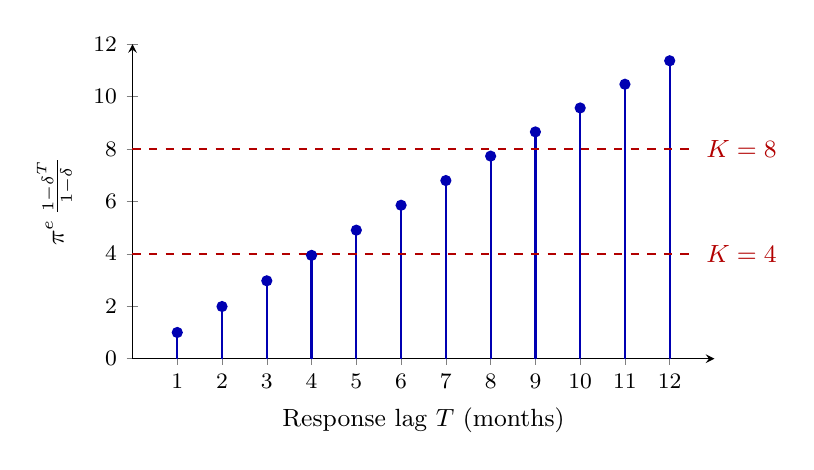
\begin{tikzpicture}
\begin{axis}[
  width=0.74\textwidth, height=0.46\textwidth,
  axis lines=left,
  xmin=0, xmax=13, ymin=0, ymax=12,
  xtick={1,2,...,12}, ytick={0,2,...,12},
  xlabel={Response lag $T$ (months)},
  ylabel={$\pi^e\,\frac{1-\delta^{T}}{1-\delta}$},
  tick label style={font=\footnotesize}, label style={font=\small},
  clip=false]
  \addplot[ycomb, thick, blue!70!black, mark=*, mark size=1.6pt, domain=1:12, samples=12]
    {(1-0.99^x)/(1-0.99)};
  \addplot[thick, dashed, red!70!black, domain=0:12.6, samples=2] {4};
  \addplot[thick, dashed, red!70!black, domain=0:12.6, samples=2] {8};
  \node[anchor=west, font=\small, red!70!black] at (axis cs:12.6,4) {$K = 4$};
  \node[anchor=west, font=\small, red!70!black] at (axis cs:12.6,8) {$K = 8$};
\end{axis}
\end{tikzpicture}
\caption{The value of hit-and-run entry when the entrant earns nothing after incumbents respond. Bars show the
discounted profit earned during a response lag of $T$ months, with $\pi^e = 1$ per month and a monthly discount
factor $\delta = 0.99$. Entry pays only if the bar reaches the sunk cost. With $K = 4$ it requires a lag of at
least 5 months, and with $K = 8$ at least 9 months. With $K = 0$ any lag makes entry profitable.}
\label{fig:09-hitrun}
\end{figure}

Airline markets have several sources of sunk costs. An entrant must set up gates, counters and other airport
facilities at a new station, and it must advertise to make itself known to local travelers. In his conclusion,
\citet[p.~362]{Borenstein1989} names advertising and the setup of airport facilities as sunk costs of entry
that may matter alongside FFPs and TACOs. Building a base of FFP members and of travel agents who book the
carrier also takes time and money that cannot be recovered on exit. The response lag is short. An incumbent
can change its fares much faster than the time that normally elapses between a rival's announcement of entry
and its first flight \citep[p.~352]{Borenstein1989}. A USAir executive testified that his carrier feared entry
but set its prices according to the competition it faced (p.~352, n.~31). In terms of
\eqref{eq:09-hitrun-closed}, incumbents can respond before the entrant's first flight, so the hit-and-run window
is empty.

\begin{remark}[Two other models of natural monopoly]\label{rem:09-other-nm}
Two models let prices adjust faster than capacity, the timing that the critique favors
\citep[secs.~8.1.2--8.1.3 and 8.6.1]{Tirole1988}. In the first, firms commit to capacity only for short periods
and set prices instantly given current capacities. There is an equilibrium in which only the incumbent
produces. It keeps renewing a capacity close to $Q(p^c)$ and earns almost no profit. With a lower capacity, an
entrant could come in, bear duopoly losses briefly, and take over once the incumbent's commitment lapses.
Tirole develops this model in his Supplementary Section 8.6.1.1.

The second is a \emph{war of attrition}. Two firms with cost $F + cq$ per unit of time are both active at
date zero, and exit is costless. While both stay, Bertrand competition sets the price at $c$, and each loses
$F$ per unit of time. A firm left alone charges $p^m$ and earns $\tilde\pi^m - F > 0$ per unit of time forever,
where $\tilde\pi^m$ is the monopoly flow profit gross of the fixed cost. In this remark only, $r$ denotes the
interest rate. In a symmetric equilibrium each firm quits at a constant hazard rate $x$, so that it is
indifferent between quitting and staying. Staying for a short time $\dd\tau$ costs $F\,\dd\tau$. With
probability $x\,\dd\tau$ the rival quits in that time, and the firm gains a monopoly worth
$\frac{\tilde\pi^m - F}{r}$. Otherwise it is again indifferent and can quit at zero value. Indifference requires
\begin{equation*}
  0 = -F\,\dd\tau + x\,\dd\tau\,\frac{\tilde\pi^m - F}{r},
  \qquad\text{so}\qquad
  x = \frac{rF}{\tilde\pi^m - F}.
\end{equation*}
In \cref{ex:09-contest}, $\tilde\pi^m = 25$ and $F = 8$, so $x = \frac{8r}{17}$. Both firms produce for a random
time, which duplicates the fixed cost, and then one exits. The price is first competitive and then equal to
the monopoly price. Firms earn no rents in expectation, and welfare is lower than under contestability.
\end{remark}

Perfect contestability makes four predictions that the empirical literature can test. Each corresponds to one
of the studies in this chapter.
\begin{enumerate}[label=(C\arabic*)]
  \item \emph{Structure does not affect fares.} Conditional on cost and demand, a route's fare does not depend
  on its concentration or on a carrier's share of the route or of its endpoint airports
  (\cref{rem:09-structure}). Earlier studies had found instead that fares on a route rise with its
  concentration \citep[p.~344]{Borenstein1989}. Borenstein cites four of these studies
  \citep{GrahamKaplanSibley1983,BaileyGrahamKaplan1985,CallKeeler1985,MorrisonWinston1987}. He regards it as
  well established that airline pricing ``does not closely reflect the perfect contestability ideal.'' \citet{BaileyGrahamKaplan1985} also found that a
  carrier's own route share raises its fares when route concentration is held fixed (p.~348, n.~18).
  \Cref{sec:09-borenstein} adds the carrier's share of its endpoint airports.
  \item \emph{Entry announcements do not hurt incumbents.} Under perfect contestability incumbents earn zero
  profit and have sunk nothing, so they have nothing to lose when an entrant appears. An announcement of entry
  should leave the incumbents' stock market values unchanged (\cref{prop:09-valueloss} below).
  \citet{WhinstonCollins1992} test this prediction (\cref{sec:09-wc}).
  \item \emph{Potential competition disciplines as much as actual competition.} The number of active rivals on
  a route should not matter once potential entrants are present (\cref{rem:09-potential}).
  \citet{Borenstein1989} includes a measure of potential competitors' presence at both endpoints of a route.
  His instrument for route share also requires that current fares respond to actual rather than potential
  rivals (p.~352). \citet{GoolsbeeSyverson2008} later study how incumbents respond to the threat of entry
  (\cref{sec:09-synthesis}).
  \item \emph{Markups only cover costs.} With two or more carriers on a route, price equals marginal cost
  (\cref{prop:09-contest-mc}). With one carrier, price equals average cost
  (\cref{prop:09-contest-monopoly}). Markups over marginal cost are positive only to the extent needed to cover
  costs that do not vary with traffic. \citet{BerryCarnallSpiller2006} estimate markups over marginal cost and
  find them higher on business travelers out of large hubs (\cref{sec:09-bcs}). Positive markups do not by
  themselves refute contestability, since average cost exceeds marginal cost when costs fall with segment
  density (\cref{rem:09-markups-profits}). Markups that differ systematically across carriers serving the same
  market are harder to reconcile with the theory.
\end{enumerate}

\subsection{Entry with sunk costs: what an incumbent's value loss reveals}\label{sec:09-entry-sunk}

Prediction (C2) can be tested without estimating demand or cost, by observing how incumbents' values change
when entry is announced. Consider an incumbent carrier on route $t$. Let $\Pi^0$ be the expected present value
of its future operating profits on the route just before an unanticipated entry announcement. Operating profit
is revenue minus all avoidable costs, including the opportunity cost of aircraft and other assets that could be
redeployed elsewhere. Let $\Pi^1$ be the same present value just after the announcement. Let $K \ge 0$ be the
incumbent's investment specific to the route that is already sunk, such as local advertising or airport
facilities. The incumbent's \emph{route value}, its economic profit on the route, counts this investment as a
cost:
\begin{equation}\label{eq:09-routevalue}
  V^0 = \Pi^0 - K, \qquad V^1 = \Pi^1 - K.
\end{equation}
The incumbent can always exit and avoid every remaining cost, so optimal behavior after the announcement gives
$\Pi^1 \ge 0$. Equivalently, $V^1 \ge -K$. The change in the firm's market value at the announcement is the
loss
\begin{equation}\label{eq:09-loss}
  L = \Pi^0 - \Pi^1 = V^0 - V^1,
\end{equation}
since the sunk investment is the same before and after.

\begin{proposition}[What a value loss reveals]\label{prop:09-valueloss}
The loss satisfies $L \le V^0 + K$. Hence $L > 0$ implies $V^0 + K > 0$: before entry the incumbent earned
positive economic profits on the route, or it had sunk costs there, or both. Under perfect contestability
$V^0 = 0$ and $K = 0$, so $L \le 0$.
\end{proposition}

\begin{proof}
From \eqref{eq:09-loss} and $V^1 \ge -K$,
\begin{equation*}
  L = V^0 - V^1 \le V^0 - (-K) = V^0 + K.
\end{equation*}
If $L > 0$, then $V^0 + K \ge L > 0$. Under perfect contestability no cost is sunk, so $K = 0$, and
\cref{prop:09-contest-zero} gives $V^0 = 0$. Hence $L \le 0$.
\end{proof}

The sum $V^0 + K = \Pi^0$ is the incumbent's pre-entry \emph{quasi-rent}, the value of operating the route over and
above all avoidable costs. A measured loss is a lower bound on it. \citet[p.~447]{WhinstonCollins1992} state the
argument in words. Suppose incumbents lose value when entry is announced. Then either ``the incumbents could
have been earning positive profits prior to entry,'' or ``they must have had sunk costs that kept them in the
market despite taking these losses.'' They estimate that the average incumbent on a route entered by People Express lost
between \$3.7 million and \$6.5 million at the announcement (p.~452), as \cref{sec:09-wc} explains.

\begin{remark}[A low-cost entrant]\label{rem:09-lowcost}
The bound holds whatever the entrant's costs. An entrant with lower costs than the incumbents violates
condition (i) of \cref{def:09-contestable} by itself. A positive loss says more. By revealing profits or sunk
costs that existed before entry, it shows that the market would not have been contestable even without the
entrant's innovation \citep[p.~447]{WhinstonCollins1992}. For the same reason the argument does not require the
entrant's low prices to be justified by its costs (p.~454, n.~23).
\end{remark}

\begin{remark}[Localization]\label{rem:09-localization}
Suppose the loss falls only on carriers that serve the entered route, while other carriers lose nothing. Then
the rents or sunk costs are tied to operations on that route. This reveals more than the sensitivity of a
route's fares to its structure. It also shows that sunk costs or other barriers to mobility prevent profits from
being equalized across routes \citep[pp.~447--448]{WhinstonCollins1992}. If airports in the same city compete
closely, carriers that serve the same city pair from other airports should lose as well.
\end{remark}

\begin{remark}[Measured losses understate the true loss]\label{rem:09-anticipation}
Suppose investors assigned probability $\varphi_0 \in [0,1)$ to entry before the announcement. The pre-announcement
value of the route was then $\varphi_0\,\Pi^1 + (1-\varphi_0)\,\Pi^0$, and after the announcement it is $\Pi^1$. The
measured change is
\begin{equation*}
  \varphi_0\,\Pi^1 + (1-\varphi_0)\,\Pi^0 - \Pi^1 = (1-\varphi_0)\,(\Pi^0 - \Pi^1) = (1-\varphi_0)\,L,
\end{equation*}
which is smaller than $L$. Misdating an event and sharing rents with workers or debtholders also bias the
measured loss toward zero \citep[p.~453]{WhinstonCollins1992}. Other forces can bias it upward, such as news
about the entrant's future expansion that affects every carrier. \Cref{sec:09-wc} shows how
\citeauthor{WhinstonCollins1992} separate such general effects from the effect of incumbency.
\end{remark}

A positive loss reveals rents but not how they arise or how incumbents respond. Static oligopoly theory
predicts the responses. Consider $N$ symmetric Cournot incumbents with inverse demand $P(Q) = a - bQ$, where
$a > c$ and $b > 0$, and constant marginal cost $c$. Firm $i$ chooses $q_i$ to maximize
\begin{equation*}
  \pi_i = \big(a - bQ - c\big)\,q_i, \qquad Q = \sum_{k=1}^N q_k .
\end{equation*}
The first-order condition is
\begin{equation*}
  a - bQ - c - b\,q_i = 0 .
\end{equation*}
Summing over the $N$ firms gives
\begin{equation*}
  N(a - c) - bNQ - bQ = 0, \qquad\text{so}\qquad Q = \frac{N(a-c)}{b(N+1)} .
\end{equation*}
By symmetry each firm produces $\frac{Q}{N}$. Substituting into the price and the profit gives the equilibrium
\begin{equation}\label{eq:09-cournot-entry}
  q^* = \frac{a-c}{b(N+1)}, \qquad
  P^* = a - \frac{N(a-c)}{N+1} = \frac{a + Nc}{N+1}, \qquad
  \pi^* = (P^* - c)\,q^* = \frac{(a-c)^2}{b(N+1)^2}.
\end{equation}
The middle expression uses $P^* - c = \frac{a-c}{N+1}$. When one firm enters, $N$ becomes $N+1$ and
\begin{equation*}
  \frac{q^*(N+1)}{q^*(N)} = \frac{N+1}{N+2}, \qquad
  P^*(N) - P^*(N+1) = \frac{a-c}{(N+1)(N+2)}, \qquad
  \frac{\pi^*(N+1)}{\pi^*(N)} = \left(\frac{N+1}{N+2}\right)^2 .
\end{equation*}
Each incumbent's output falls, the price falls, and each incumbent's profit falls. Total output rises from
$\frac{N(a-c)}{b(N+1)}$ to $\frac{(N+1)(a-c)}{b(N+2)}$. \Cref{sec:02-cournot} proves these comparative statics
for general demand.

An entrant like People Express brings lower costs. The next result shows that a cost advantage makes the
incumbents' losses larger.

\begin{proposition}[Entry by a low-cost firm]\label{prop:09-cournot-entrant}
In the linear Cournot model, let one entrant with marginal cost $c_e \le c$ join the $N$ incumbents, and
suppose all firms produce positive output after entry. Then each incumbent produces
$\frac{a - 2c + c_e}{b(N+2)}$ and earns $\frac{(a - 2c + c_e)^2}{b(N+2)^2}$. Its output, the price and its
profit are lower than before entry, and they fall further as $c_e$ falls.
\end{proposition}

\begin{proof}
The incumbents' first-order conditions are $a - bQ - c - b\,q = 0$, and the entrant's is
$a - bQ - c_e - b\,q_e = 0$. Summing the $N+1$ conditions gives
\begin{equation*}
  N(a-c) + (a - c_e) - b(N+1)Q - bQ = 0, \qquad\text{so}\qquad
  Q = \frac{N(a-c) + (a - c_e)}{b(N+2)} .
\end{equation*}
The price is
\begin{equation*}
  P = a - bQ = \frac{(N+2)a - N(a-c) - (a - c_e)}{N+2} = \frac{a + Nc + c_e}{N+2}.
\end{equation*}
An incumbent's first-order condition gives $b\,q = P - c$, so
\begin{equation*}
  q = \frac{a + Nc + c_e - (N+2)c}{b(N+2)} = \frac{a - 2c + c_e}{b(N+2)}, \qquad
  \pi = (P - c)\,q = b\,q^2 = \frac{(a - 2c + c_e)^2}{b(N+2)^2}.
\end{equation*}
Before entry, $q^* = \frac{a-c}{b(N+1)}$. Because $c_e \le c$, $a - 2c + c_e \le a - c$, and
$\frac{1}{N+2} < \frac{1}{N+1}$. Hence $q < q^*$, and $\pi = bq^2 < b(q^*)^2 = \pi^*$. The price
$\frac{a + Nc + c_e}{N+2}$ is below $\frac{a + Nc}{N+1}$ because $c_e \le c < a$. All three expressions increase
in $c_e$.
\end{proof}

The source of entry matters for what an incumbent's loss reveals. \citet[p.~447, n.~4]{WhinstonCollins1992}
illustrate the point with a simple model of entry with sunk costs, such as that of \citet{MankiwWhinston1986}.
In such a model, entry triggered by an innovation of the entrant lowers incumbents' values. Entry triggered by a shock to demand or to costs
common to all firms can raise or lower them. The linear model makes the point precise.

\begin{proposition}[Innovation versus demand shocks]\label{prop:09-entry-source}
In the linear Cournot model, let $N$ firms be active under free entry with sunk entry cost $K$. Free entry means
$\pi^*(N) \ge K > \pi^*(N+1)$, where $\pi^*(N) = \frac{(a-c)^2}{b(N+1)^2}$. (a) If entry occurs because one
potential entrant's marginal cost falls to $c_e < c$, each incumbent's profit flow falls. (b) If entry occurs
because demand rises from $a$ to $a' > a$, with $\frac{(a'-c)^2}{b(N+2)^2} \ge K$, each incumbent's profit flow
changes from $\frac{(a-c)^2}{b(N+1)^2}$ to $\frac{(a'-c)^2}{b(N+2)^2}$. It rises if and only if
$\frac{a'-c}{a-c} > \frac{N+2}{N+1}$. If $a'$ is the smallest demand level at which the $(N+1)$th firm enters, it
does not rise.
\end{proposition}

\begin{proof}
Part (a) is \cref{prop:09-cournot-entrant}. For part (b), the incumbent's new profit flow follows from
\eqref{eq:09-cournot-entry} with $N+1$ firms and intercept $a'$. Comparing the square roots of the two profit
flows gives the stated condition. If $a'$ is the smallest intercept at which the $(N+1)$th firm enters, then
$\frac{(a'-c)^2}{b(N+2)^2} = K \le \pi^*(N)$.
\end{proof}

The proposition explains why entry by a single innovative carrier is a clean experiment. When entry follows
an entrant-specific innovation, the market's reaction measures the loss from entry itself. When it follows
news about demand on the route, the same reaction mixes the loss with the good news. People Express was widely
seen as a carrier with new products and lower costs, so its announcements fit case (a). The fit is imperfect.
\citet[p.~459]{WhinstonCollins1992} acknowledge that changes in demand or costs on a route could themselves have
prompted entry.

\begin{remark}[Capacities and the Kreps-Scheinkman result]\label{rem:09-ks}
Airlines commit to schedules, and hence to seat capacity, before they set fares. \citet{KrepsScheinkman1983}
show that capacity choice followed by price competition yields the Cournot outcome, under concave demand and
efficient rationing (\cref{prop:02-ks}). The comparative statics of \eqref{eq:09-cournot-entry} and
\cref{prop:09-cournot-entrant} then apply to capacities. Entry should lead incumbents to cut capacity and sales
along with price. \citet[p.~460]{WhinstonCollins1992} make this point and find the opposite. Incumbents on routes
entered by People Express appear to have raised their seats offered and their sales after entry
(\cref{sec:09-wc}).
\end{remark}

When can entry raise an incumbent's output in a static model? Consider Cournot competition with general inverse
demand $P(Q)$ and cost $C(q_i)$. Write $Q_{-i}$ for the rivals' total output. Firm $i$'s first-order condition is
\begin{equation*}
  P(q_i + Q_{-i}) + q_i\,P'(q_i + Q_{-i}) - C'(q_i) = 0 .
\end{equation*}
Differentiating with respect to $Q_{-i}$ and writing $q_i' = \frac{\dd q_i}{\dd Q_{-i}}$ gives
\begin{equation*}
  P'\,(q_i' + 1) + P'\,q_i' + q_i\,P''\,(q_i' + 1) - C''\,q_i' = 0 .
\end{equation*}
Collecting the terms in $q_i'$,
\begin{equation}\label{eq:09-br-slope}
  q_i' = -\,\frac{P' + q_i P''}{2P' + q_i P'' - C''} .
\end{equation}
The second-order condition makes the denominator negative. The best response therefore slopes up exactly when
$P' + q_i P'' > 0$. In the language of \citet{BulowGeanakoplosKlemperer1985}, quantities are then
\emph{strategic complements}. This requires demand convex enough that $P'' > -\frac{P'}{q_i} > 0$. With linear
demand, $P'' = 0$ and quantities are strategic substitutes. An incumbent that answers entry with more output
and capacity thus contradicts the standard static models unless demand is unusually convex.
\citet[p.~460]{WhinstonCollins1992} suggest a dynamic interpretation instead. Incumbents may have responded
aggressively in the hope of inducing the entrant to exit, or at least of discouraging its further expansion.

Contestability theory tells us when market power cannot exist. It is silent on how market power shows up
in fares when the theory fails. Answering that question requires a model of pricing on a route, with
several carriers, differentiated products, heterogeneous travelers and network costs. The next section
builds this model. It supplies the structural reading of the fare regressions of \cref{sec:09-borenstein}
and the model that \cref{sec:09-bcs} estimates.

\section{Market power in airline markets: pricing theory}\label{sec:09-pricing}

The three empirical studies in this chapter rest on one body of pricing theory, which this section
develops in four steps. First, we derive a route-level pricing equation from a homogeneous-goods model
with a conduct parameter. This equation gives a structural reading of the fare regressions of
\cref{sec:09-borenstein}. Second, we show that airport dominance can raise a carrier's markup through
product differentiation alone, with no softening of rivals' behavior. Third, we build the finite-mixture
nested logit with $R$ consumer types that \citet{BerryCarnallSpiller2006} estimate. We derive its
shares, substitution patterns, markups and inversion. Fourth, we model costs on a network, where the
marginal cost of a passenger depends on traffic density on each flight leg, and we derive the pricing
condition of a network carrier.

Markets, carriers and products are those of \cref{sec:09-data}. A market $t$ is a directional
origin-destination pair, carriers are firms $f=1,\dots,F$, and $\mathcal{J}_t$ is the set of inside
products in market $t$. We add one piece of notation: $\mathcal{J}_f(t)\subseteq\mathcal{J}_t$ collects
the products that carrier $f$ sells in market $t$.

\subsection{From conduct to a route-level pricing equation}\label{sec:09-pricing-conduct}

We start from the simplest model that links fares to market structure. It treats travel on a route as a
homogeneous good and summarizes each carrier's behavior by a conduct parameter, as in \cref{ch:theory}
and \cref{ch:conduct}.

\begin{assumption}[Homogeneous route market]\label{ass:09-homog}
On route $t$, carriers $f=1,\dots,F$ sell a homogeneous product with outputs $q_{ft}$ and total output
$Q_t=\sum_f q_{ft}$. Inverse demand $P(Q_t)$ is differentiable and strictly decreasing, and the market
elasticity is $\varepsilon_t=-\frac{P(Q_t)}{Q_tP'(Q_t)}>0$. Carrier $f$ has constant marginal cost
$mc_{ft}$ and share $s_{ft}=\frac{q_{ft}}{Q_t}$.
\end{assumption}

\begin{definition}[Firm-level conduct]\label{def:09-conduct}
The \emph{conduct parameter} $\theta_{ft}$ of carrier $f$ on route $t$ is the number that satisfies
\begin{equation}\label{eq:09-conduct-foc}
P(Q_t)\left(1-\frac{\theta_{ft}}{\varepsilon_t}\right)=mc_{ft},
\qquad\text{equivalently}\qquad
L_{ft}\equiv\frac{P(Q_t)-mc_{ft}}{P(Q_t)}=\frac{\theta_{ft}}{\varepsilon_t}.
\end{equation}
\end{definition}

The benchmarks follow from a conjectural-variations first-order condition. Suppose carrier $f$ chooses
$q_{ft}$ and conjectures that rivals' total output $Q_{-f,t}=Q_t-q_{ft}$ responds as
$\frac{\dd Q_{-f,t}}{\dd q_{ft}}=v_{ft}$. Its first-order condition is
\begin{equation*}
P(Q_t)+q_{ft}P'(Q_t)\,(1+v_{ft})-mc_{ft}=0 .
\end{equation*}
Dividing by $P(Q_t)$ and using the definitions of $s_{ft}$ and $\varepsilon_t$,
\begin{equation*}
\frac{P-mc_{ft}}{P}
=-\frac{q_{ft}P'(Q_t)}{P}\,(1+v_{ft})
=\frac{q_{ft}}{Q_t}\left(-\frac{Q_tP'(Q_t)}{P}\right)(1+v_{ft})
=\frac{s_{ft}(1+v_{ft})}{\varepsilon_t}.
\end{equation*}
Hence $\theta_{ft}=s_{ft}(1+v_{ft})$. Cournot conjectures ($v_{ft}=0$) give $\theta_{ft}=s_{ft}$, which
equals $\frac{1}{N}$ with $N$ symmetric firms. Price taking gives $\theta_{ft}=0$. When all carriers have
the same cost, joint profit maximization sets $\frac{P-mc}{P}=\frac{1}{\varepsilon_t}$, so
$\theta_{ft}=1$.

We parametrize conduct between Cournot and joint profit maximization as
\begin{equation}\label{eq:09-theta-param}
\theta_{ft}=s_{ft}+\eta_t\,(1-s_{ft}),\qquad \eta_t\in[0,1].
\end{equation}
Matching $\theta_{ft}=s_{ft}(1+v_{ft})$ gives $v_{ft}=\eta_t\frac{1-s_{ft}}{s_{ft}}=\eta_t\frac{Q_{-f,t}}{q_{ft}}$,
which rearranges to $\frac{\dd Q_{-f,t}}{Q_{-f,t}}=\eta_t\frac{\dd q_{ft}}{q_{ft}}$. Carrier $f$ therefore
expects rivals to change their output by $\eta_t$ percent when it changes its own by one percent. We call
$\eta_t$ the \emph{collusiveness} of route $t$. With $\eta_t=0$ carriers play Cournot, and with
$\eta_t=1$ every carrier prices as a joint monopolist would.

\casehead{The pricing equation}
Write $p_t=P(Q_t)$ for the route price and take logs of \eqref{eq:09-conduct-foc}:
\begin{equation*}
\ln p_t=\ln mc_{ft}-\ln\left(1-\frac{\theta_{ft}}{\varepsilon_t}\right).
\end{equation*}
The expansion $-\ln(1-x)=x+\frac{x^2}{2}+\frac{x^3}{3}+\cdots$ gives $-\ln(1-x)\approx x$ when
$x=\frac{\theta_{ft}}{\varepsilon_t}$ is small, so
\begin{equation*}
\ln p_t\approx\ln mc_{ft}+\frac{\theta_{ft}}{\varepsilon_t}.
\end{equation*}
Substituting \eqref{eq:09-theta-param},
\begin{align}
\ln p_t&\approx\ln mc_{ft}+\frac{s_{ft}+\eta_t(1-s_{ft})}{\varepsilon_t}\notag\\
&=\ln mc_{ft}+\frac{\eta_t}{\varepsilon_t}+\frac{1-\eta_t}{\varepsilon_t}\,s_{ft}.
\label{eq:09-pricing-approx}
\end{align}
The approximation is accurate for moderate Lerner indices. At $\frac{\theta_{ft}}{\varepsilon_t}=0.2$ the
exact term is $-\ln 0.8=0.223$, against $0.2$ for the linear term, so the linear form slightly understates
large markups.

Equation \eqref{eq:09-pricing-approx} splits the log price into three parts. The first is marginal cost.
The second, $\frac{\eta_t}{\varepsilon_t}$, is a route-level markup shared by every carrier. The third is
an own-share term with slope $\frac{1-\eta_t}{\varepsilon_t}$. Under Cournot conduct the slope is
$\frac{1}{\varepsilon_t}$ and the route-level term vanishes. Under joint profit maximization the slope is
zero, and every carrier's markup reflects only $\frac{1}{\varepsilon_t}$. The share coefficient therefore
falls as conduct becomes more collusive.

\casehead{The umbrella hypothesis}
The \emph{umbrella hypothesis} holds that a dominant carrier's high fares shelter its smaller rivals,
which can then price above their competitive level. A natural way to formalize it is to let concentration
raise collusiveness,
\begin{equation}\label{eq:09-umbrella-eta}
\eta_t=\eta_0+\eta_1\HHI_t,\qquad \eta_1>0,
\end{equation}
where $\HHI_t=\sum_f s_{ft}^2$ is the route Herfindahl index. Substituting \eqref{eq:09-umbrella-eta}
into \eqref{eq:09-pricing-approx} and collecting terms,
\begin{align}
\ln p_t&\approx\ln mc_{ft}+\frac{\eta_0+\eta_1\HHI_t}{\varepsilon_t}
+\frac{1-\eta_0-\eta_1\HHI_t}{\varepsilon_t}\,s_{ft}\notag\\
&=\ln mc_{ft}+\frac{\eta_0}{\varepsilon_t}+\frac{1-\eta_0}{\varepsilon_t}\,s_{ft}
+\frac{\eta_1}{\varepsilon_t}\,\HHI_t-\frac{\eta_1}{\varepsilon_t}\,\HHI_t\,s_{ft}.
\label{eq:09-umbrella}
\end{align}
The effect of concentration on a carrier's price is
$\frac{\partial\ln p_t}{\partial\HHI_t}=\frac{\eta_1(1-s_{ft})}{\varepsilon_t}$. It is largest for the
carriers with the smallest shares, which is exactly what an umbrella means.

Equation \eqref{eq:09-umbrella} maps into the market-power block of Borenstein's pricing equation
\eqref{eq:09-bor-price}, which omits the interaction $\HHI_t\,s_{ft}$. Let $\bar H$ and $\bar s$ be the
sample means of $\HHI_t$ and $s_{ft}$. Linearizing the interaction around them gives
$\HHI_ts_{ft}\approx\bar H s_{ft}+\bar s\HHI_t-\bar s\bar H$. Holding the elasticity fixed, the
route-share coefficient (RUTSHARE) is then $\phi_3\approx\frac{1-\eta_0-\eta_1\bar H}{\varepsilon}$. The
route-Herfindahl coefficient (RUTHERF) is $\phi_4\approx\frac{\eta_1(1-\bar s)}{\varepsilon}$. The
umbrella hypothesis still predicts $\phi_4>0$, and $\eta_1=0$ still gives $\phi_4=0$. In Borenstein's
sample $\bar H=0.50$ and $\bar s=0.54$ \citep[Table~4]{Borenstein1989}, so $\phi_4$ is less than half of
$\frac{\eta_1}{\varepsilon}$. Variation in $\varepsilon_t$ across routes makes all three coefficients
averages as well, which is one reason to control for the tourist share of a route's travelers.

\casehead{Share-weighted margins}
Multiplying the Lerner index $L_{ft}=\frac{\theta_{ft}}{\varepsilon_t}$ by $s_{ft}$ and summing over
carriers gives the route's share-weighted margin:
\begin{align}
\sum_f s_{ft}L_{ft}
&=\frac{1}{\varepsilon_t}\sum_f s_{ft}\big[s_{ft}+\eta_t(1-s_{ft})\big]
=\frac{1}{\varepsilon_t}\Big[\sum_f s_{ft}^2+\eta_t\Big(\sum_f s_{ft}-\sum_f s_{ft}^2\Big)\Big]\notag\\
&=\frac{(1-\eta_t)\HHI_t+\eta_t}{\varepsilon_t}.\label{eq:09-cowling}
\end{align}
With $\eta_t=0$ this is the result $\frac{\HHI_t}{\varepsilon_t}$ of \citet{CowlingWaterson1976}
(\cref{prop:02-cowling-waterson}). Under Cournot conduct, share-weighted margins rise with concentration even when
conduct is identical on every route. A cross-route regression of margins on $\HHI_t$ in the
structure-conduct-performance tradition (\cref{ch:intro}) therefore finds a positive slope without any
umbrella effect. Under joint profit maximization ($\eta_t=1$) the share-weighted margin is
$\frac{1}{\varepsilon_t}$ whatever the concentration.

\casehead{Functional form}
Equation \eqref{eq:09-pricing-approx} explains the functional form that the airline pricing literature
adopted. Profit maximization makes price proportional to marginal cost times an inverse-elasticity term,
so the cost part enters in logs \citep[p.~354]{Borenstein1989}. Borenstein parametrizes $\ln mc_{ft}$
by a carrier effect, the log of nonstop distance and logs of cost and quality variables such as load
factor, aircraft size, frequency and circuity. Shares and Herfindahl indices enter linearly. Borenstein
motivates the linear share with an example \citep[p.~354]{Borenstein1989}. A rise in share from 1\% to 2\%
should not have the same effect as a rise from 30\% to 60\%. Our derivation adds a theoretical reason: to
first order, the log price is linear in the share. \citet{BaileyGrahamKaplan1985} had already included the observed carrier's route share and found a
positive effect after controlling for route concentration \citep[p.~348, n.~18]{Borenstein1989}.
Borenstein describes his equation as a supply relation in the framework of \citet{Bresnahan1989}. The cost function is never estimated separately. It is
inferred from cross-sectional variation in prices and product attributes \citep[p.~348, n.~18]{Borenstein1989},
as in \cref{ch:conduct}.

\begin{remark}[What the share coefficient can and cannot reveal]\label{rem:09-share-coef}
Borenstein's \emph{two-stage least squares} (2SLS) estimates of $\phi_3$ range from $0.029$ for the median fare to
$0.224$ for the 80th percentile fare \citep[Table~2]{Borenstein1989}. Equation
\eqref{eq:09-umbrella} reads these numbers as $\frac{1-\bar\eta}{\varepsilon}$, where
$\bar\eta=\eta_0+\eta_1\bar H$ is the collusiveness at the mean Herfindahl index. A Cournot reading
with $\bar\eta=0$ requires market elasticities $\varepsilon=\frac{1}{\phi_3}$ between about $4.5$ and
$35$. A market elasticity of $1.5$ instead requires $\bar\eta=1-1.5\,\phi_3$, between $0.66$ and $0.96$,
which is close to joint profit maximization. Small share coefficients are thus consistent either with
elastic route demand or with nearly collusive conduct. Without an independent estimate of $\varepsilon$
the regression cannot tell the two apart. This is the identification problem of \cref{ch:conduct} in a
new setting.
\end{remark}

Two features of airline markets strain the homogeneous-goods model and motivate the rest of this section.
First, the model predicts a single price on each route. Carriers on the same route charge different
fares, and each sells many fares. Borenstein's relative-price equation \eqref{eq:09-bor-rel} compares two
carriers' fares on the same route, and in the homogeneous model its left side is identically zero. With
a common price, \eqref{eq:09-pricing-approx} also forces carriers with larger shares to have lower
marginal costs. Second, a large share may reflect a better product or a lower cost rather than market
power. \citet{Demsetz1973} made this argument for concentration across industries (\cref{ch:intro}).
In the homogeneous model the share is a sufficient statistic for cost efficiency. When costs are measured
with error, the share coefficient absorbs the unmeasured part of cost. In a differentiated market, a
carrier with a more attractive product has both a larger share and a higher price, so the share
coefficient also absorbs quality. Instruments for the share, such as Borenstein's GENPSH
(\cref{sec:09-borenstein}), address the simultaneity of share and price. They cannot separate market
power from quality when the two are the same thing, as the next model shows.

\subsection{Dominance as product differentiation: markups without an umbrella}\label{sec:09-pricing-diff}

Many of the sources of airport dominance described in \cref{sec:09-dominance-sources} work through
demand.
A frequent-flyer program is worth more when the carrier flies to more places from the traveler's home
airport. Frequency, convenient gates and a local reputation make a carrier's flights more attractive.
\citet{Berry1990} treats airport presence as a source of product differentiation in this sense. We now model
dominance as higher non-price quality and ask what it implies for prices.

\begin{assumption}[Logit route market]\label{ass:09-logit}
Route $t$ (subscript dropped) has single-product carriers $j=1,\dots,J$ and an outside good $j=0$.
Consumer $i$ has utility $u_{ij}=\delta_j-\alpha p_j+\epsilon_{ij}$ for $j\ge1$ and $u_{i0}=\epsilon_{i0}$,
with $\epsilon_{ij}$ i.i.d.\ type-I extreme value and $\alpha>0$. Carrier $j$ has constant marginal cost
$c_j$ and chooses $p_j$ to maximize $(p_j-c_j)Ms_j(p)$, taking rivals' prices as given.
\end{assumption}

In this subsection only, $\delta_j$ denotes the non-price part of mean utility ($x_j\beta+\xi_j$ in the
notation of \cref{ch:logit}), so that mean utility including price is $\delta_j-\alpha p_j$. Shares and
own-price derivatives are (\cref{ch:logit})
\begin{equation*}
s_j=\frac{e^{\delta_j-\alpha p_j}}{1+\sum_{k=1}^J e^{\delta_k-\alpha p_k}},
\qquad
\frac{\partial s_j}{\partial p_j}=-\alpha s_j(1-s_j).
\end{equation*}
The first-order condition $s_j+(p_j-c_j)\frac{\partial s_j}{\partial p_j}=0$ becomes
$s_j-\alpha(p_j-c_j)s_j(1-s_j)=0$. Dividing by $\alpha s_j(1-s_j)$,
\begin{equation}\label{eq:09-logit-markup}
p_j-c_j=\frac{1}{\alpha(1-s_j)} .
\end{equation}

\begin{proposition}[Dominance without an umbrella]\label{prop:09-dominance}
Under \cref{ass:09-logit} the Bertrand-Nash equilibrium exists and is unique. In equilibrium:
\begin{enumerate}[label=(\roman*)]
\item Each carrier's markup $p_j-c_j=\frac{1}{\alpha(1-s_j)}$ is strictly increasing in its own share, so
carriers with larger shares charge larger markups.
\item An increase in $\delta_1$ raises $p_1$ and $s_1$, lowers the outside share $s_0$, and lowers $p_k$
and $s_k$ for every rival $k\neq1$.
\end{enumerate}
\end{proposition}

\begin{proof}
Part (i) is immediate from \eqref{eq:09-logit-markup}. For part (ii) and for existence and uniqueness we
reduce the equilibrium to a single equation in $s_0$.

\emph{Step 1 (one equation per carrier).} Let $m_j=p_j-c_j$ and $a_j=e^{\delta_j-\alpha c_j}$. The
first-order condition \eqref{eq:09-logit-markup} is $s_j=1-\frac{1}{\alpha m_j}$, which requires
$m_j>\frac{1}{\alpha}$. The logit formula gives
$\frac{s_j}{s_0}=e^{\delta_j-\alpha p_j}=a_je^{-\alpha m_j}$. Substituting the first-order condition
into the logit ratio,
\begin{equation*}
1-\frac{1}{\alpha m_j}=s_0\,a_je^{-\alpha m_j},
\qquad\text{so}\qquad
h(m_j)\equiv\Big(1-\frac{1}{\alpha m_j}\Big)e^{\alpha m_j}=s_0\,a_j .
\end{equation*}

\emph{Step 2 ($h$ is invertible).} On $\big(\frac{1}{\alpha},\infty\big)$, $h$ is continuous, $h$ tends
to $0$ as $m\downarrow\frac{1}{\alpha}$, and $h(m)\to\infty$ as $m\to\infty$. Its derivative is
\begin{equation*}
h'(m)=e^{\alpha m}\Big[\frac{1}{\alpha m^2}+\alpha-\frac{1}{m}\Big]
=e^{\alpha m}\,\frac{(\alpha m)^2-\alpha m+1}{\alpha m^2}>0,
\end{equation*}
because $x^2-x+1=\big(x-\frac{1}{2}\big)^2+\frac{3}{4}>0$. Hence $m_j=h^{-1}(s_0a_j)$ is strictly
increasing in $s_0a_j$. The share is $s_j=S(s_0a_j)$ with
$S(y)\equiv1-\frac{1}{\alpha h^{-1}(y)}$, which is continuous and strictly increasing, with $S(y)\to0$ as
$y\to0$ and $S(y)\to1$ as $y\to\infty$.

\emph{Step 3 (existence and uniqueness).} Shares add up to one:
\begin{equation*}
G(s_0;a)\equiv s_0+\sum_{j=1}^J S(s_0a_j)=1 .
\end{equation*}
$G$ is continuous and strictly increasing in $s_0$, with $G(0;a)=0$ and $G(1;a)>1$. A unique
$s_0^*\in(0,1)$ solves the equation, and Step 2 then gives unique markups and shares. Any equilibrium
satisfies the first-order conditions, so there is at most one equilibrium. The first-order conditions
are also sufficient. Given rivals' prices, the left side of $p_j-c_j=\frac{1}{\alpha(1-s_j(p))}$ rises in
$p_j$ while the right side falls, because $s_j$ falls in $p_j$. Profit therefore rises below the unique
crossing and falls above it, so the crossing is the best response.

\emph{Step 4 (comparative statics).} A higher $\delta_1$ raises $a_1$. Since $S$ is increasing,
$G(s_0;a)$ rises at every $s_0$, so the solution $s_0^*$ falls. For each $k\neq1$, the product
$s_0^*a_k$ falls, so $m_k$ and $s_k$ fall, and $p_k=c_k+m_k$ falls. Finally
$s_1=1-s_0^*-\sum_{k\neq1}s_k$ rises because $s_0^*$ and every $s_k$ fall. Then
$m_1=\frac{1}{\alpha(1-s_1)}$ rises and so does $p_1=c_1+m_1$.
\end{proof}

The existence and uniqueness result agrees with the general results for logit-type demand in
\cref{ch:diffprod} \citep{CaplinNalebuff1991}. The single-equation reduction is useful in its own right,
since it computes the equilibrium by solving one monotone equation. \Cref{fig:09-dominance} uses it.

\begin{figure}[htbp]
\centering
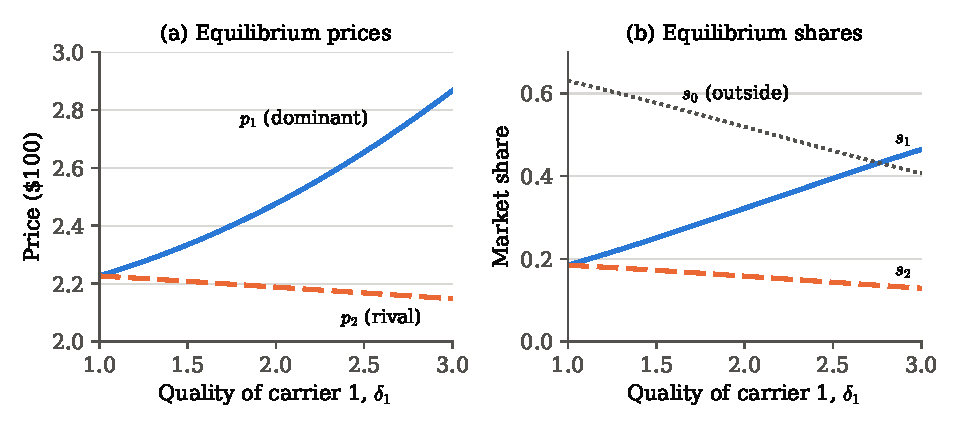
\includegraphics[width=\textwidth]{figures/ch09/logit_dominance.pdf}
\caption{Logit Bertrand equilibrium on a route with two carriers and an outside good, as carrier 1's
non-price quality $\delta_1$ rises. Parameters are $\alpha=1$ (prices in \$100), $c_1=c_2=1$ and
$\delta_2=1$. At $\delta_1=1$ both carriers charge $2.227$. At $\delta_1=3$, $p_1=2.867$, $p_2=2.148$,
$s_1=0.464$ and $s_2=0.129$. The dominant carrier's price rises while its rival's falls.}
\label{fig:09-dominance}
\end{figure}

\Cref{fig:09-dominance} traces the equilibrium of a two-carrier route as carrier 1's quality rises from
$\delta_1=1$ to $\delta_1=3$. Carrier 1's share rises from $0.185$ to $0.464$ and its price from $2.227$
to $2.867$. The rival's share falls from $0.185$ to $0.129$ and its price from $2.227$ to $2.148$.
The Herfindahl index of inside shares rises from $0.500$ to $0.660$. Concentration rises and the rival's
price falls, the opposite of an umbrella. Logit prices are strategic complements, so carrier 1's higher
price alone would push $p_2$ up. The loss of customers to the better product outweighs this effect, and
the rival's markup $\frac{1}{\alpha(1-s_2)}$ falls with its share.

\begin{corollary}[Relative prices]\label{cor:09-relprice}
Under \cref{ass:09-logit}, an increase in $\delta_1$ raises $\ln p_1-\ln p_k$ for every $k\neq1$. Along
any path of shares, $\frac{\dd\ln p_j}{\dd s_j}=\frac{L_j}{1-s_j}$, where $L_j=\frac{p_j-c_j}{p_j}$ is
the Lerner index. With equal costs, $\ln p_1-\ln p_k\approx\frac{L}{1-s}\,(s_1-s_k)$ for shares near a
common value $s$ with Lerner index $L$.
\end{corollary}

\begin{proof}
The first claim follows from \cref{prop:09-dominance}(ii), since $p_1$ rises and $p_k$ falls. For the
slope, differentiate \eqref{eq:09-logit-markup}:
$\frac{\dd m_j}{\dd s_j}=\frac{1}{\alpha(1-s_j)^2}=\frac{m_j}{1-s_j}$. Then
$\frac{\dd\ln p_j}{\dd s_j}=\frac{1}{p_j}\frac{\dd m_j}{\dd s_j}=\frac{m_j}{p_j}\frac{1}{1-s_j}=\frac{L_j}{1-s_j}$.
A first-order expansion around the common share gives the approximation.
\end{proof}

The corollary is the structural counterpart of Borenstein's relative-price equation
\eqref{eq:09-bor-rel}. There, the coefficient on the difference in route shares between two carriers on
the same route plays the role of $\frac{L(1-s_0)}{1-s}$. Route shares are shares of fliers,
$\frac{s_j}{1-s_0}$, so the gap in route shares between carriers 1 and $k$ is $\frac{s_1-s_k}{1-s_0}$.
A positive coefficient is what product differentiation
predicts, with no change in conduct. In the example of \cref{fig:09-dominance}, $\ln p_1-\ln p_2$ rises
from $0$ to $0.289$ as $\delta_1$ goes from 1 to 3.

\begin{remark}[Quality or cost?]\label{rem:09-quality-cost}
The equilibrium depends on $(\delta_j,c_j)$ only through $a_j=e^{\delta_j-\alpha c_j}$. A cost advantage
therefore has the same effect on shares and markups as a quality advantage of $\alpha$ times the cost
gap. In the example of \cref{fig:09-dominance}, $(\delta_1,c_1)=(1.5,1)$ and $(\delta_1,c_1)=(1,0.5)$
give identical shares ($s_1=0.251$, $s_2=0.172$) and the same markup $m_1=1.334$. Only carrier 1's price
differs, $2.334$ against $1.834$. A relation between shares and markups cannot reveal whether dominance
comes from quality or from cost. Separating them requires a model of costs, which is what
\cref{sec:09-pricing-network} and \cref{sec:09-bcs} provide.
\end{remark}

\casehead{Multi-product carriers}
A carrier usually sells several products on a route: direct and connecting itineraries, and several fare
classes. With logit demand, the first-order condition for $j\in\mathcal{J}_f$ is
$s_j-\alpha s_jm_j+\alpha s_j\sum_{k\in\mathcal{J}_f}s_km_k=0$. Dividing by $\alpha s_j$ gives
$m_j=\frac{1}{\alpha}+\sum_{k\in\mathcal{J}_f}s_km_k$. The right side does not depend on $j$, so all of
the carrier's products carry a common markup $m_f$. Substituting back,
$m_f=\frac{1}{\alpha}+S_fm_f$, so
\begin{equation*}
m_f=\frac{1}{\alpha(1-S_f)},\qquad S_f=\sum_{k\in\mathcal{J}_f}s_k
\end{equation*}
(\cref{ch:logit}). Summing the logit ratios over the carrier's products gives
$\frac{S_f}{s_0}=A_fe^{-\alpha m_f}$ with $A_f=\sum_{k\in\mathcal{J}_f}a_k$. The proof of
\cref{prop:09-dominance} then applies with carriers in place of products and $A_f$ in place of $a_j$.
A carrier with a large total share on the route earns a large markup on every product it sells there.

The logit model also has a limitation that matters for airlines. Every product of a carrier carries the
same dollar markup, whether it is a restricted discount ticket or an unrestricted fare. Characteristics
affect the markup only through shares. The model cannot express the idea that a hub lets its carrier
raise fares mainly to business travelers. That requires heterogeneity in price sensitivity, to which we
now turn.

\subsection{Consumer heterogeneity: a finite-mixture nested logit}\label{sec:09-pricing-types}

Air travelers differ in ways that matter for pricing. Business travelers are less sensitive to price
\citep[p.~10, n.~9]{BerryCarnallSpiller2006}. Their trips are urgent, travel is a deductible business
expense, and the traveler may not bear the full cost of the ticket. They may also value frequency, nonstop service and
frequent-flyer benefits more, so tastes are correlated across characteristics. A model in which the
price coefficient and the tastes vary across consumers lets markups differ across the products of one
carrier. It also lets a hub's demand advantage fall on particular travelers.
Earlier discrete choice models of air travel, such as that of \citet{MorrisonWinston1986}, used a
logit with common coefficients \citep[p.~8]{BerryCarnallSpiller2006}. \citet{BerryCarnallSpiller2006}
adopt the simplest distribution with heterogeneous tastes, a two-point distribution of types. We develop the model with $R$ types and specialize to $R=2$ in \cref{sec:09-bcs}.

\begin{assumption}[Finite-mixture nested logit]\label{ass:09-fm}
Market $t$ has $M_t$ potential travelers. Each belongs to one of $R$ types, and type $r$ has population
share $\psi_r>0$ with $\sum_r\psi_r=1$. A traveler $i$ of type $r$ has utility
\begin{equation*}
u_{ijt}=x_{jt}\beta_r-\alpha_rp_{jt}+\xi_{jt}+\zeta_{igt}+(1-\sigma)\epsilon_{ijt}
\quad (j\in\mathcal{J}_t),\qquad u_{i0t}=\epsilon_{i0t}.
\end{equation*}
The shocks $\epsilon_{ijt}$ are i.i.d.\ type-I extreme value. All inside goods form one nest $g$ and the
outside good forms its own nest. The term $\zeta_{igt}$ is common to all inside goods for traveler $i$
and has the distribution of \citet{Cardell1997}, which makes $\zeta_{igt}+(1-\sigma)\epsilon_{ijt}$
type-I extreme value, with $\sigma\in[0,1)$. The unobserved quality $\xi_{jt}$ is common to all types.
\end{assumption}

The nesting parameter $\sigma$ measures the correlation of a traveler's utilities across flights. With
$\sigma=0$ the model is a mixture of logits, and as $\sigma\to1$ flights become perfect substitutes for
one another relative to the outside good (\cref{ch:logit}, \cref{ch:discrete}). Berry, Carnall and
Spiller write the idiosyncratic term as $\lambda\epsilon_{ij}$, so their $\lambda$ equals $1-\sigma$.
In applications $M_t$ is unobserved. They set $M_t=\kappa\,\mathit{MPOP}_t$, with $\mathit{MPOP}_t$ the
geometric mean of the endpoint populations and $\kappa$ a parameter to be estimated
\citep[p.~9]{BerryCarnallSpiller2006}.

\begin{remark}[Discrete random coefficients]\label{rem:09-discrete-rc}
The type structure is a random coefficients logit (\cref{ch:blp}) whose mixing distribution has $R$
support points $(\alpha_r,\beta_r)$ with probabilities $\psi_r$. Normal random coefficients are the usual
alternative. Suppose $K$ coefficients, price included, vary across consumers. Two types then require
$2K+1$ parameters, two values per coefficient plus $\psi_1$, against $2K$ for independent normals with a
mean and a standard deviation each \citep[p.~11]{BerryCarnallSpiller2006}. In exchange the shares have a
closed form and no simulation is needed. A two-point distribution is bimodal and makes tastes correlated
across characteristics by construction. The price is that it has no taste variation within a type.
Mixtures of normals or more types would relax this but require numerical integration or many more
parameters.
\end{remark}

\casehead{Shares}
Fix a market and write $\delta^r_{jt}$ for the mean utility of type $r$, which includes price as in
\cref{ch:logit}. Conditional on type, the model is a nested logit, so
\begin{subequations}\label{eq:09-fm-shares}
\begin{align}
\delta^r_{jt}&=x_{jt}\beta_r-\alpha_rp_{jt}+\xi_{jt},\\
D_{rt}&=\sum_{k\in\mathcal{J}_t}\exp\Big(\frac{\delta^r_{kt}}{1-\sigma}\Big),\\
s^r_{j|g,t}&=\frac{1}{D_{rt}}\exp\Big(\frac{\delta^r_{jt}}{1-\sigma}\Big),\\
\bar s_{rt}&=\frac{D_{rt}^{1-\sigma}}{1+D_{rt}^{1-\sigma}},\\
s^r_{jt}&=s^r_{j|g,t}\,\bar s_{rt},\\
s_{jt}&=\sum_{r=1}^R\psi_r\,s^r_{jt}.
\end{align}
\end{subequations}
Here $s^r_{j|g,t}$ is the probability that a type-$r$ traveler chooses $j$ given that she flies, and
$\bar s_{rt}$ is the probability that she flies at all. The last line averages over types by the law of
total probability. The outside share is $s_{0t}=\sum_r\frac{\psi_r}{1+D_{rt}^{1-\sigma}}$. The
\emph{inclusive sum} $D_{rt}$ is the denominator of type $r$'s within-nest shares. It carries a type
subscript and should not be confused with the diversion ratio $D_{jk}$ below, which carries two product
subscripts. In the rest of this subsection we drop the market subscript.

\casehead{Derivatives}
We differentiate the type-specific shares with respect to type-specific mean utilities and then convert
to prices. From \eqref{eq:09-fm-shares},
\begin{equation*}
\ln s^r_j=\frac{\delta^r_j}{1-\sigma}-\ln D_r+(1-\sigma)\ln D_r-\ln\big(1+D_r^{1-\sigma}\big)
=\frac{\delta^r_j}{1-\sigma}-\sigma\ln D_r-\ln\big(1+D_r^{1-\sigma}\big).
\end{equation*}
The two building blocks are
\begin{equation*}
\frac{\partial\ln D_r}{\partial\delta^r_k}=\frac{1}{1-\sigma}\,\frac{1}{D_r}\exp\Big(\frac{\delta^r_k}{1-\sigma}\Big)
=\frac{s^r_{k|g}}{1-\sigma},
\qquad
\frac{\partial\ln\big(1+D_r^{1-\sigma}\big)}{\partial\delta^r_k}
=\bar s_r\,(1-\sigma)\,\frac{\partial\ln D_r}{\partial\delta^r_k}=\bar s_r\,s^r_{k|g}=s^r_k .
\end{equation*}
Therefore
\begin{equation*}
\frac{\partial\ln s^r_j}{\partial\delta^r_k}
=\frac{\indic\{j=k\}}{1-\sigma}-\frac{\sigma}{1-\sigma}\,s^r_{k|g}-s^r_k .
\end{equation*}
Multiplying by $s^r_j$ and using $s^r_j\,s^r_{k|g}=s^r_k\,s^r_{j|g}$ gives the own and cross derivatives.
Since $\frac{\partial\delta^r_k}{\partial p_k}=-\alpha_r$, the price derivatives of aggregate shares
follow:
\begin{subequations}\label{eq:09-fm-derivs}
\begin{align}
\frac{\partial s^r_j}{\partial\delta^r_j}&=s^r_j\Big[\frac{1}{1-\sigma}-\frac{\sigma}{1-\sigma}\,s^r_{j|g}-s^r_j\Big],\\
\frac{\partial s^r_j}{\partial\delta^r_k}&=-s^r_k\Big[\frac{\sigma}{1-\sigma}\,s^r_{j|g}+s^r_j\Big],\qquad k\neq j,\\
\frac{\partial s_j}{\partial p_k}&=-\sum_{r=1}^R\psi_r\,\alpha_r\,\frac{\partial s^r_j}{\partial\delta^r_k}.
\end{align}
\end{subequations}
The matrix of type-specific derivatives is symmetric, so $\frac{\partial s_j}{\partial p_k}=\frac{\partial
s_k}{\partial p_j}$ in this model. Own-price derivatives are negative and cross-price derivatives are
positive.

\casehead{Buyer composition}
Bayes' rule gives the composition of each product's buyers:
\begin{equation}\label{eq:09-composition}
\Pr(r\mid j)=\frac{\psi_r\,s^r_{jt}}{s_{jt}} .
\end{equation}
The numerator is the probability of being type $r$ and buying $j$, and the denominator is the
probability of buying $j$. Berry, Carnall and Spiller use these weights to compute average fares,
costs and markups by type (\cref{sec:09-bcs}). With them, the own-price elasticity and the diversion
ratio take a transparent form. Dividing \eqref{eq:09-fm-derivs} by $s_j$,
\begin{align*}
\varepsilon_{jj}&=-\frac{\partial s_j}{\partial p_j}\,\frac{p_j}{s_j}
=p_j\sum_r\Pr(r\mid j)\,\alpha_r\Big[\frac{1}{1-\sigma}-\frac{\sigma}{1-\sigma}\,s^r_{j|g}-s^r_j\Big],\\
D_{jk}&=-\frac{\frac{\partial s_k}{\partial p_j}}{\frac{\partial s_j}{\partial p_j}}
=\frac{\sum_r\Pr(r\mid j)\,\alpha_r\Big[\frac{\sigma}{1-\sigma}\,s^r_{k|g}+s^r_k\Big]}
{\sum_r\Pr(r\mid j)\,\alpha_r\Big[\frac{1}{1-\sigma}-\frac{\sigma}{1-\sigma}\,s^r_{j|g}-s^r_j\Big]} .
\end{align*}
A product bought mostly by price-insensitive types has a low elasticity even at a high price. This breaks
the logit's implication that elasticities rise in proportion to price (\cref{ch:logit}). Diversion from
$j$ to $k$ is high when the types who buy $j$ are the types for whom $k$ has a large share. Two cheap
tickets bought by the same price-sensitive travelers are therefore close substitutes, whatever their
aggregate shares.

\begin{proposition}[Who pays the premium]\label{prop:09-composition-markup}
Under \cref{ass:09-fm} with $\sigma=0$, suppose carrier $f$ sells the single product $j$ in market $t$
and sets its price as in Nash-Bertrand equilibrium.
\begin{enumerate}[label=(\alph*)]
\item The markup is
\begin{equation*}
p_j-mc_j=\frac{s_j}{\sum_r\psi_r\alpha_rs^r_j(1-s^r_j)}=\frac{1}{\sum_r\Pr(r\mid j)\,\alpha_r(1-s^r_j)} .
\end{equation*}
\item Let $R=2$. Holding all prices fixed, a marginal increase in a characteristic $x^h_j$ of product $j$
raises the share of type-2 buyers $\Pr(2\mid j)$ if and only if
$\beta^h_2(1-s^2_j)>\beta^h_1(1-s^1_j)$.
\end{enumerate}
\end{proposition}

\begin{proof}
(a) The first-order condition is $s_j+(p_j-mc_j)\frac{\partial s_j}{\partial p_j}=0$. With $\sigma=0$,
\eqref{eq:09-fm-derivs} gives $\frac{\partial s_j}{\partial p_j}=-\sum_r\psi_r\alpha_rs^r_j(1-s^r_j)$.
Solving for the markup gives the first expression. Dividing numerator and denominator by $s_j$ and using
\eqref{eq:09-composition} gives the second.

(b) Write $\Pr(2\mid j)=\Big[1+\frac{\psi_1s^1_j}{\psi_2s^2_j}\Big]^{-1}$, which is increasing in
$\ln s^2_j-\ln s^1_j$. With $\sigma=0$, $\frac{\partial\ln s^r_j}{\partial\delta^r_j}=1-s^r_j$ and
$\frac{\partial\delta^r_j}{\partial x^h_j}=\beta^h_r$. Hence
$\frac{\partial(\ln s^2_j-\ln s^1_j)}{\partial x^h_j}=\beta^h_2(1-s^2_j)-\beta^h_1(1-s^1_j)$.
\end{proof}

Part (a) says that the markup is the inverse of a buyer-weighted average price sensitivity. When
type-specific shares are small, the markup is close to $\frac{1}{\bar\alpha_j}$, where
$\bar\alpha_j=\sum_r\Pr(r\mid j)\alpha_r$ is the mean price coefficient among $j$'s buyers. Part (b) says
which characteristics move the buyer mix. Combine the two with $\alpha_2<\alpha_1$. A characteristic that
type 2 values more, such as hub presence valued by business travelers, tilts $j$'s buyers toward type 2.
This lowers $\bar\alpha_j$ and raises the markup on $j$. Products bought mainly by tourists keep low
markups even when the hub carrier sells them. The hub premium thus falls on the travelers who value the
hub, which is the mechanism behind the results of \cref{sec:09-bcs}. In the logit model, by contrast,
the markup $\frac{1}{\alpha(1-s_j)}$ depends on characteristics only through the share.

\begin{remark}[Nesting and multi-product carriers]\label{rem:09-fm-extensions}
With $\sigma>0$ the same steps give
$p_j-mc_j=\Big(\sum_r\Pr(r\mid j)\,\alpha_r\Big[\frac{1}{1-\sigma}-\frac{\sigma}{1-\sigma}s^r_{j|g}-s^r_j\Big]\Big)^{-1}$.
If within-nest shares are small, the bracket is close to $\frac{1}{1-\sigma}$ and the markup is close to
$\frac{1-\sigma}{\bar\alpha_j}$. Closer substitution among flights (larger $\sigma$) lowers markups. A
product with a large within-nest share among its own buyers earns a higher markup. With multi-product
carriers the markups solve the system \eqref{eq:09-fm-markup} below. They differ across a carrier's
products according to buyer composition, unlike the common logit markup $\frac{1}{\alpha(1-S_f)}$.
\end{remark}

\casehead{Inversion}
Estimation requires the vector $\xi_t$ that rationalizes observed shares. For given demand parameters
$\theta_d=(\sigma,\{\alpha_r,\beta_r,\psi_r\}_{r=1}^R)$ and market size, \eqref{eq:09-fm-shares}
defines shares $s_t(\xi_t;\theta_d)$, and we must solve $s_t(\xi_t;\theta_d)=s^{obs}_t$ for $\xi_t$.
\citet{Berry1994} shows that this inverse exists and is unique (\cref{ch:logit}, \cref{ch:blp}).
Berry, Carnall and Spiller compute it with ``a slight variation'' of the contraction of
\citet{BerryLevinsohnPakes1995} \citep[p.~17]{BerryCarnallSpiller2006}. One natural variation dampens
the step by $1-\sigma$:
\begin{equation}\label{eq:09-fm-contraction}
\xi^{n+1}=\Phi(\xi^n),\qquad \Phi(\xi)\equiv\xi+(1-\sigma)\big[\ln s^{obs}-\ln s(\xi;\theta_d)\big].
\end{equation}
A fixed point of $\Phi$ satisfies $\ln s(\xi;\theta_d)=\ln s^{obs}$. The next lemma shows why the
dampening works.

\begin{lemma}[Contraction for the finite-mixture nested logit]\label{lem:09-fm-contraction}
At every $\xi$, all elements of the Jacobian of $\Phi$ are positive, and each row sums to
$\sum_r\Pr(r\mid j)\big[\sigma+(1-\sigma)\bar s_r\big]\le\sigma+(1-\sigma)\max_r\bar s_r<1$. Hence
$\Phi$ is a contraction in the sup norm, with modulus at most $\sigma+(1-\sigma)\bar S$, on any convex
set of $\xi$ on which every inside share satisfies $\bar s_r\le\bar S<1$.
\end{lemma}

\begin{proof}
Each $\delta^r_k$ moves one for one with $\xi_k$, so by \eqref{eq:09-fm-shares} and
\eqref{eq:09-composition}
\begin{equation*}
\frac{\partial\ln s_j}{\partial\xi_k}=\frac{1}{s_j}\sum_r\psi_rs^r_j\frac{\partial\ln s^r_j}{\partial\delta^r_k}
=\sum_r\Pr(r\mid j)\Big[\frac{\indic\{j=k\}}{1-\sigma}-\frac{\sigma}{1-\sigma}\,s^r_{k|g}-s^r_k\Big].
\end{equation*}
Multiplying by $1-\sigma$ and using $\sum_r\Pr(r\mid j)=1$,
\begin{equation*}
(1-\sigma)\frac{\partial\ln s_j}{\partial\xi_k}
=\indic\{j=k\}-\sum_r\Pr(r\mid j)\big[\sigma s^r_{k|g}+(1-\sigma)s^r_k\big].
\end{equation*}
The Jacobian of $\Phi$ is therefore
$\frac{\partial\Phi_j}{\partial\xi_k}=\sum_r\Pr(r\mid j)\big[\sigma s^r_{k|g}+(1-\sigma)s^r_k\big]>0$.
Summing over $k$ and using $\sum_ks^r_{k|g}=1$ and $\sum_ks^r_k=\bar s_r$ gives the row sum. With
positive elements, the sup norm of the Jacobian equals its largest row sum. The mean value theorem then
bounds $\|\Phi(\xi)-\Phi(\xi')\|_\infty$ by the modulus times $\|\xi-\xi'\|_\infty$ on a convex set.
\end{proof}

The set on which inside shares are bounded by $\bar S$ is convex, because $D_r$ is a convex function of
$\xi$. Applying the contraction mapping theorem (\cref{app:math}) also requires a set that $\Phi$ maps
into itself. The bounding argument of \citet{BerryLevinsohnPakes1995} supplies one (\cref{ch:blp}).
In airline city pairs, actual trips are a small fraction of potential trips. Inside shares are then
small and the modulus is close to $\sigma$, so the iteration converges quickly.

\casehead{Markups}
Within a single market, carrier $f$ chooses the prices of its products $\mathcal{J}_f(t)$ to maximize
$\sum_{j\in\mathcal{J}_f(t)}(p_j-mc_j)M_ts_j(p)$. The first-order condition for $j\in\mathcal{J}_f(t)$ is
\begin{equation*}
s_j+\sum_{k\in\mathcal{J}_f(t)}(p_k-mc_k)\frac{\partial s_k}{\partial p_j}=0 .
\end{equation*}
Let $\Omega$ be the ownership matrix and $\Delta$ the matrix with $(j,k)$ element
$\frac{\partial s_j}{\partial p_k}$ (\cref{ch:diffprod}). The $(j,k)$ element of
$(\Omega\odot\Delta)^\top$ is $\Omega_{kj}\frac{\partial s_k}{\partial p_j}$, so stacking the conditions
gives
\begin{equation}\label{eq:09-fm-markup}
s+(\Omega\odot\Delta)^\top(p-mc)=0
\quad\Longrightarrow\quad
p-mc=-\big[(\Omega\odot\Delta)^\top\big]^{-1}s,
\qquad
\Delta=-\sum_{r=1}^R\psi_r\,\alpha_r\,\frac{\partial s^r}{\partial\delta^r},
\end{equation}
where $\frac{\partial s^r}{\partial\delta^r}$ is the matrix with $(j,k)$ element
$\frac{\partial s^r_j}{\partial\delta^r_k}$ from \eqref{eq:09-fm-derivs}.\footnote{Berry, Carnall and
Spiller define $\Delta$ with $(j,k)$ element $\frac{\partial s_k}{\partial p_j}$ for products of the same
carrier and write $p=\Delta^{-1}s+mc$ \citep[pp.~15--16]{BerryCarnallSpiller2006}. The equation holds when
$\Delta$ contains the negatives of the price derivatives. Their formula
$\Delta=\gamma\alpha_1\Delta_1+(1-\gamma)\alpha_2\Delta_2$, with $\Delta_r$ the derivatives with respect to
mean utility and $\gamma$ the type-1 probability, delivers exactly these negatives, since
$\frac{\partial s^r}{\partial p}=-\alpha_r\frac{\partial s^r}{\partial\delta^r}$.} In this model $\Omega$
and $\Delta$ are both symmetric, so the transpose is immaterial. It matters for general demand systems.
The markups depend only on the demand parameters and on observed prices and shares. Given demand
estimates, marginal cost follows as $mc=p+\big[(\Omega\odot\Delta)^\top\big]^{-1}s$, without any cost
data.

\casehead{How aggregate data identify types}
Berry, Carnall and Spiller explain how market-level data can distinguish two consumer types from one
\citep[pp.~18--19]{BerryCarnallSpiller2006}. The key is variation across markets in the number of similar
products. The following example makes their argument quantitative.

\begin{example}[Two types from aggregate shares]\label{ex:09-twotypes}
Consider two city pairs, A and B, identical in every respect except their sets of products. Products are
identical except for price. Market A has a product $H$ at \$200 and a product $L$ at \$100. Market B has
$H$ at \$200 and two products $L_1$ and $L_2$ at \$100. In market A we observe $s_H=s_L$.

\emph{One type.} In a nested logit with a single type, within-nest shares are proportional to
$\exp\big(\frac{\delta_j}{1-\sigma}\big)$. Equal shares in market A therefore imply $\delta_H=\delta_L$. In market B
the three products then have equal mean utilities and equal shares, for any $\alpha$ and $\sigma$. The
same conclusion holds in any model whose error is additive and i.i.d.\ across products
\citep[p.~18]{BerryCarnallSpiller2006}.

\emph{Two types.} Let $\alpha_1=3$ and $\alpha_2=0.1$ per \$100, $\psi_1=0.9$, $\sigma=0.4$ and
$\delta^r_j=\xi_j-\alpha_rp_j$ with $\xi_L=0$. Setting $\xi_H=0.903$ equates the two shares in market A
at $0.0567$. In market A, $97\%$ of type 1's flights are on $L$, while $79\%$ of type 2's flights are on
$H$. Adding $L_2$ in market B splits type 1's demand for cheap flights and barely touches type 2's demand
for $H$. Market B shares become $0.0483$ for $H$ and $0.0438$ for each cheap product, so $H$'s share is
$10\%$ above each of the others (\cref{tab:09-twotypes}, \cref{fig:09-twotypes}). Under one type every
product loses $17.5\%$ of its share when $L_2$ enters. Under two types $H$ loses $14.7\%$ and $L$ loses
$22.7\%$.

The substitution patterns explain the difference. In market B, $28\%$ of each cheap product's buyers are
type 2, against $98\%$ of $H$'s buyers. A rise in the price of $L_1$ diverts $0.277$ of its lost sales to
$L_2$ and only $0.017$ to $H$. A one-type model would divert equal fractions to $L_2$ and $H$. The farther
apart $\alpha_1$ and $\alpha_2$, the larger the gap between the shares of $H$ and $L$ in market B. Data
with many such comparisons across markets therefore pin down the dispersion of price coefficients.

\emph{Which type values hubs?} Now add a hub characteristic $x^h_j$ with type-specific coefficients
$\beta^h_r$. Differentiating \eqref{eq:09-fm-shares} as in \cref{lem:09-fm-contraction},
\begin{equation*}
\frac{\partial\ln s_j}{\partial x^h_j}=\sum_r\Pr(r\mid j)\,\beta^h_r\,\frac{\partial\ln s^r_j}{\partial\delta^r_j},
\end{equation*}
a buyer-weighted average of type-specific responses. In market A, with $(\beta^h_1,\beta^h_2)=(0.2,1.0)$
the semi-elasticities are $0.579$ for $H$ and $0.499$ for $L$. With $(\beta^h_1,\beta^h_2)=(1.0,0.2)$ they
are $0.151$ for $H$ and $0.794$ for $L$. How the shares of cheap and expensive products respond to hub
presence thus reveals which type has the large hub coefficient \citep[p.~19]{BerryCarnallSpiller2006}.
\end{example}

\begin{table}[htbp]
\centering
\caption{Two-type identification example: market shares and buyer composition}
\label{tab:09-twotypes}
\begin{tabular}{lcccccc}
\toprule
 & & Market A & \multicolumn{2}{c}{Market B} & \multicolumn{2}{c}{$\Pr(r=2\mid j)$}\\
\cmidrule(lr){4-5}\cmidrule(lr){6-7}
Product & Price (\$) & both models & one type & two types & A & B\\
\midrule
$H$ & 200 & 0.0567 & 0.0467 & 0.0483 & 0.977 & 0.980\\
$L$ in A, $L_1$ in B & 100 & 0.0567 & 0.0467 & 0.0438 & 0.256 & 0.284\\
$L_2$ & 100 & & 0.0467 & 0.0438 & & 0.284\\
Outside good & & 0.8867 & 0.8598 & 0.8641 & & \\
\bottomrule
\end{tabular}

\smallskip
\begin{minipage}{0.92\textwidth}
\footnotesize Notes: Both models are calibrated to reproduce market A exactly. The two-type model has
$\alpha_1=3$, $\alpha_2=0.1$ (per \$100), $\psi_1=0.9$, $\sigma=0.4$, $\xi_L=0$ and $\xi_H=0.903$. The
one-type model is a nested logit with the same $\sigma$. Our computations.
\end{minipage}
\end{table}

\begin{figure}[htbp]
\centering
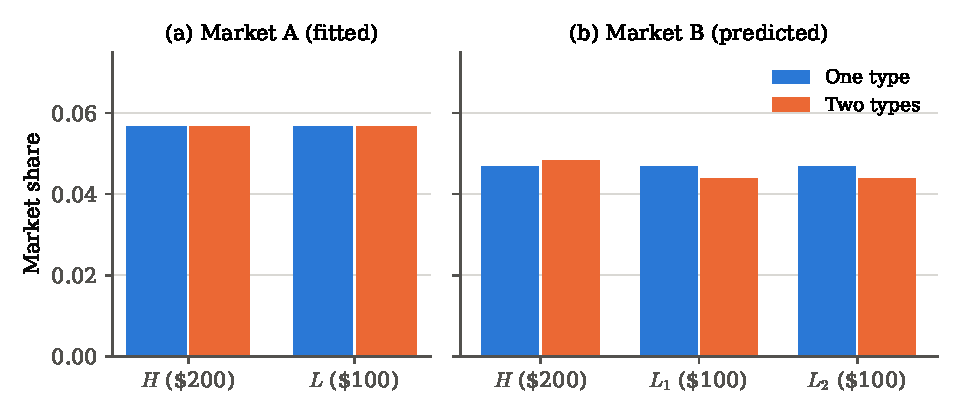
\includegraphics[width=\textwidth]{figures/ch09/twotypes_example.pdf}
\caption{Identifying two types from aggregate shares. Both models fit market A, where the \$200 and
\$100 products have equal shares. In market B, which adds a second \$100 product, the one-type model
predicts three equal shares. The two-type model predicts that the expensive product keeps more of its
share, because the two cheap products compete for the same price-sensitive travelers. Parameters as in
\cref{tab:09-twotypes}.}
\label{fig:09-twotypes}
\end{figure}

\begin{remark}[The role of nesting in the example]\label{rem:09-twotypes-sigma}
The direction of the departure from the one-type prediction depends on the whole specification. With
$\sigma=0$ and the same $\alpha_r$ and $\psi_r$, recalibrating $\xi_H$ to fit market A gives market B
shares of $0.0530$ for $H$ and $0.0576$ for each cheap product. Without nesting, flights compete mainly
with the outside good. Type 2 values every flight highly because $\alpha_2$ is small, so it gives the new
cheap product a larger share than type 1 does, and $H$ loses more. The nesting parameter makes flights
compete with one another within each type. What identifies the types is the existence of departures from
the one-type prediction, and the data determine their direction.
\end{remark}

Random coefficients also change how markups respond to entry. Berry, Carnall and Spiller stress that with
random coefficients, introducing similar products drives markups down \citep[p.~18]{BerryCarnallSpiller2006}.
In \cref{ex:09-twotypes}, the inverse semi-elasticity of $L$'s demand,
$-s_L\big(\frac{\partial s_L}{\partial p_L}\big)^{-1}$, is the markup a single-product seller of $L$ would choose. It falls from $0.453$ (\$45) in market A
to $0.352$ (\$35) in market B, because $L_2$ competes for exactly the travelers who buy $L$. A one-type
nested logit with the same $\sigma$ predicts a fall of only 9\%, which comes from the decline in $L$'s
shares alone.

\subsection{Network costs and economies of density}\label{sec:09-pricing-network}

The cost side of hubbing rests on an engineering argument. Larger aircraft are cheaper to fly per seat
mile, at least on longer routes \citep[pp.~3--4]{BerryCarnallSpiller2006}. For a given flight frequency, a
densely traveled spoke can use larger aircraft. A hub combines passengers bound for many destinations
on one large aircraft to the hub, where they change planes. We first define the relevant cost concepts,
then work through a stylized network, and finally derive the pricing condition of a network carrier.

\begin{definition}[Returns to density and to scale]\label{def:09-rtd}
Let $C(Q,P,w)$ be a carrier's total cost, with traffic $Q$ (for example passenger miles), number of
points served $P$ and input prices $w$. Write $\varepsilon_{CQ}=\frac{\partial\ln C}{\partial\ln Q}$ and
$\varepsilon_{CP}=\frac{\partial\ln C}{\partial\ln P}$. \emph{Returns to density} and \emph{returns to
scale} are
\begin{equation}\label{eq:09-rtd}
RTD=\frac{1}{\varepsilon_{CQ}},\qquad RTS=\frac{1}{\varepsilon_{CQ}+\varepsilon_{CP}} .
\end{equation}
\end{definition}

Returns to density measure the cost of adding traffic to a fixed network, and returns to scale the cost
of expanding traffic and the network together. Since $\varepsilon_{CQ}=\frac{Q}{C}\frac{\partial C}{\partial Q}$, the density elasticity also equals the ratio of marginal to average cost of traffic.
\citet{CavesChristensenTretheway1984} estimate an airline cost function \citep[p.~4]{BerryCarnallSpiller2006}.
Holding the route structure fixed, total cost rises only 80\% as fast as traffic. This means $\varepsilon_{CQ}\approx0.8$ and
$RTD\approx\frac{1}{0.8}=1.25$. Berry, Carnall and Spiller point out two limits of this approach. An
aggregate cost function ignores details of route structure that determine densities. Holding the number
of endpoints fixed, for instance, densities fall as a carrier operates more hubs
\citep[p.~4, n.~7]{BerryCarnallSpiller2006}. And route-level cost data do not exist, since route-level
total or average cost is not even well defined. \citet{BruecknerSpiller1994} instead model the marginal
cost of a passenger on each leg as a function of that leg's density and sum over the legs of an
itinerary. They find that funneling passengers through hub airports raised traffic densities and let
carriers reduce costs \citep[pp.~4--5]{BerryCarnallSpiller2006}. \citet{BruecknerDyerSpiller1992} make
the related point that itineraries through a hub may have lower costs because they raise spoke density
\citep[p.~2]{BerryCarnallSpiller2006}. Berry, Carnall and Spiller adopt the leg-level approach.

\begin{example}[Hub-and-spoke versus point-to-point costs]\label{ex:09-hubcost}
A carrier serves $n$ outer cities and one hub city. Every pair of the $n+1$ cities has $A$ round-trip
passengers. Each leg has cost $C(Q)=aQ^\gamma$ with $0<\gamma\le1$, so legs have \emph{economies of
density}, marginal and average cost falling with traffic, when $\gamma<1$. All legs have equal length and we ignore circuity.

\emph{Point to point.} Every city pair gets a nonstop leg. There are $\frac{n(n+1)}{2}$ legs, each
carrying density $A$, so
\begin{equation*}
C^{PP}=\frac{n(n+1)}{2}\,aA^\gamma .
\end{equation*}

\emph{Hub and spoke.} There are $n$ spokes. The spoke from outer city $e$ carries the $A$ passengers
between $e$ and the hub and the $A$ passengers between $e$ and each of the other $n-1$ outer cities. Its
density is $A+(n-1)A=nA$, so
\begin{equation*}
C^{HS}=n\,a(nA)^\gamma=aA^\gamma\,n^{1+\gamma} .
\end{equation*}

\emph{Comparison.} Dividing,
\begin{equation*}
\frac{C^{HS}}{C^{PP}}=\frac{aA^\gamma n^{1+\gamma}}{\frac{n(n+1)}{2}aA^\gamma}=\frac{2n^\gamma}{n+1} .
\end{equation*}
Hubbing is cheaper if and only if $2n^\gamma<n+1$. With $\gamma=1$ this requires $n<1$, so hubbing is
never cheaper: connecting passengers fly two legs instead of one. With $n=10$ and $\gamma=0.7$ the ratio
is $\frac{2\times10^{0.7}}{11}=\frac{10.02}{11}=0.91$. For $\gamma=0.7$ hubbing lowers total cost once
$n\ge7$, and for $\gamma=0.8$ once $n\ge27$.

\emph{Marginal costs.} Leg marginal cost is $c(Q)=a\gamma Q^{\gamma-1}$. A nonstop passenger in the
point-to-point network costs $a\gamma A^{\gamma-1}$. A connecting passenger in the hub network flies two
spokes of density $nA$ and costs $2a\gamma(nA)^{\gamma-1}$, a ratio of $2n^{\gamma-1}$. A passenger
to or from the hub flies one spoke, a ratio of $n^{\gamma-1}<1$. With $n=10$ and $\gamma=0.7$ the
connecting ratio is $1.00$ and the hub-endpoint ratio is $0.50$.
\end{example}

\begin{figure}[htbp]
\centering
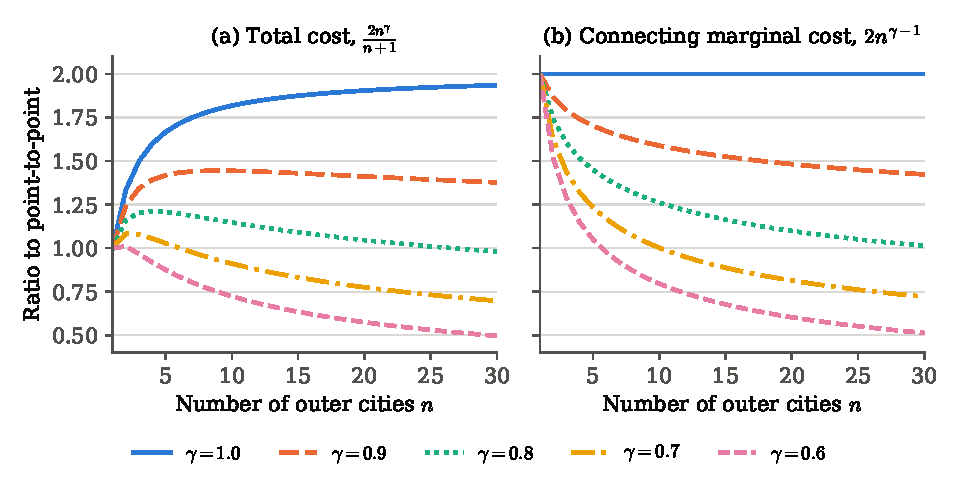
\includegraphics[width=\textwidth]{figures/ch09/hubcost_ratio.pdf}
\caption{Hub-and-spoke relative to point-to-point costs in \cref{ex:09-hubcost}, as functions of the
number of outer cities $n$ for several leg cost elasticities $\gamma$. Panel (a) shows total network cost,
panel (b) the marginal cost of a connecting passenger. Values below the dashed line favor the hub.}
\label{fig:09-hubcost}
\end{figure}

\Cref{fig:09-hubcost} plots both ratios. Three lessons emerge. Economies of density are necessary for a
hub to save cost in this setting, because connecting passengers use two legs. The savings grow with the
size of the network, since each spoke pools more city pairs. And passengers who start or end at the hub
have the lowest marginal cost, because they use one dense spoke. This last point anticipates the finding
of \cref{sec:09-bcs} that carriers with large hubs have lower marginal costs on flights out of their hubs.
The firm-level elasticity of 0.8 is not the same object as the leg-level $\gamma$. If the two were equal,
hubbing would lower total cost in this stylized network only with at least 27 outer cities. The example
ignores the extra distance of connecting trips, the value of frequency, congestion at the hub and the
fact that many thin city pairs would get no nonstop service at all.

\casehead{Itinerary marginal cost}
Let $\mathcal{L}_f$ be the set of legs (spokes) that carrier $f$ flies. As in \cref{sec:09-data},
$\mathcal{L}(j)$ is the set of legs in the itinerary of product $j$. The density $Q_\ell$ of leg $\ell$
counts the passengers on all itineraries that use it, in every market \eqref{eq:09-density}. Legs are
carrier specific, so only carrier $f$'s products contribute to the density of a leg in $\mathcal{L}_f$.
Leg $\ell$ has total cost $C_\ell(Q_\ell,w_\ell)$ and marginal cost
$c_\ell(Q_\ell,w_\ell)=\frac{\partial C_\ell}{\partial Q_\ell}$, where $w_\ell$ collects exogenous leg
characteristics such as distance and airport congestion. Following \citet{BruecknerSpiller1994}, the
marginal cost of product $j$ is the sum of its legs' marginal costs plus a product-specific shock
$\omega_j$:
\begin{equation}\label{eq:09-itin-mc}
mc_j=\sum_{\ell\in\mathcal{L}(j)}c_\ell(Q_\ell,w_\ell)+\omega_j .
\end{equation}
The carrier's total cost is
\begin{equation}\label{eq:09-firm-cost}
C_f=\sum_{\ell\in\mathcal{L}_f}C_\ell(Q_\ell,w_\ell)+\sum_t\ \sum_{j\in\mathcal{J}_f(t)}\omega_jq_j+FC_f ,
\end{equation}
where $FC_f$ is fixed cost. The term $\omega_jq_j$ exists only to give marginal cost an additive error
\citep[p.~13]{BerryCarnallSpiller2006}. Legs are shared by many products, so a product's total cost is
undefined while its marginal cost is well defined. Shared legs create economies of scope across itineraries.
The itinerary New York-Chicago-San Diego shares a spoke with New York-Chicago-Seattle. More demand for New
York-San Diego raises traffic on the New York-Chicago leg \citep[p.~2, n.~5]{BerryCarnallSpiller2006}. With
economies of density, the extra traffic lowers the marginal cost of serving New York-Seattle.

\casehead{The pricing condition of a network carrier}
Assume that demand in market $t$ depends only on the prices of products in market $t$. Using
\eqref{eq:09-firm-cost}, carrier $f$'s profit is
\begin{equation*}
\pi_f=\sum_t\ \sum_{j\in\mathcal{J}_f(t)}(p_j-\omega_j)\,q_j(p)-\sum_{\ell\in\mathcal{L}_f}C_\ell(Q_\ell,w_\ell)-FC_f .
\end{equation*}
Differentiate with respect to the price of a product $j\in\mathcal{J}_f(t)$. Products in other markets do
not respond to $p_j$, so the revenue terms give
$q_j+\sum_{k\in\mathcal{J}_f(t)}(p_k-\omega_k)\frac{\partial q_k}{\partial p_j}$. The cost terms give
$-\sum_{\ell\in\mathcal{L}_f}c_\ell(Q_\ell,w_\ell)\frac{\partial Q_\ell}{\partial p_j}$, with
\begin{equation*}
\frac{\partial Q_\ell}{\partial p_j}=\sum_{k\in\mathcal{J}_f(t):\,\ell\in\mathcal{L}(k)}\frac{\partial q_k}{\partial p_j}.
\end{equation*}
Exchanging the order of summation over legs and products,
\begin{equation*}
\sum_{\ell\in\mathcal{L}_f}c_\ell\sum_{k\in\mathcal{J}_f(t):\,\ell\in\mathcal{L}(k)}\frac{\partial q_k}{\partial p_j}
=\sum_{k\in\mathcal{J}_f(t)}\frac{\partial q_k}{\partial p_j}\sum_{\ell\in\mathcal{L}(k)}c_\ell .
\end{equation*}
Collecting terms and using \eqref{eq:09-itin-mc},
\begin{equation}\label{eq:09-network-foc}
\frac{\partial\pi_f}{\partial p_j}
=q_j+\sum_{k\in\mathcal{J}_f(t)}\Big[p_k-\omega_k-\sum_{\ell\in\mathcal{L}(k)}c_\ell(Q_\ell,w_\ell)\Big]\frac{\partial q_k}{\partial p_j}
=q_j+\sum_{k\in\mathcal{J}_f(t)}(p_k-mc_k)\frac{\partial q_k}{\partial p_j}=0 .
\end{equation}
This is the condition of \citet[p.~15]{BerryCarnallSpiller2006}.

Equation \eqref{eq:09-network-foc} has the same form as the single-market condition behind
\eqref{eq:09-fm-markup}. The network enters only through the level of each $mc_k$, evaluated at
network-wide equilibrium densities. A lower price in market $t$ raises density on the legs its products
share with other markets. With economies of density this lowers the marginal cost of the carrier's
products elsewhere, and those products are repriced in turn. Equilibrium prices are therefore linked
across all markets that share legs, even though each first-order condition involves one market only. For
estimation, \eqref{eq:09-fm-markup} and \eqref{eq:09-itin-mc} combine into
$p_j-\text{markup}_j(\theta_d)=\sum_{\ell\in\mathcal{L}(j)}c_\ell(Q_\ell,w_\ell)+\omega_j$, a regression of
price net of markup on leg cost terms.

Densities are endogenous in that regression. A product with high unobserved demand $\xi$ raises the
density of its legs, which lowers marginal cost when there are economies of density. Demand shocks thus
move density and price together, and shocks to $\omega$ may be correlated across products that share
legs. Estimation must instrument for density with variables that shift traffic on a leg but not product
costs. Berry, Carnall and Spiller use population and network characteristics of the endpoint cities
(\cref{sec:09-bcs}).

\begin{remark}[Markups are not profits]\label{rem:09-markups-profits}
Let a leg have cost $C_\ell(Q)=F_\ell+aQ^\gamma$ with $F_\ell\ge0$ and $\gamma<1$. Average cost is
$\frac{F_\ell}{Q}+aQ^{\gamma-1}$ and marginal cost is $\gamma aQ^{\gamma-1}$, so
\begin{equation*}
AC-MC=\frac{F_\ell}{Q}+(1-\gamma)aQ^{\gamma-1}>0 .
\end{equation*}
Pricing at marginal cost loses $Q(AC-MC)=F_\ell+(1-\gamma)aQ^\gamma$. At the break-even price $p=AC$, the
Lerner index is $1-\frac{MC}{AC}$. With $F_\ell=0$ this equals $1-\gamma$. More generally, at $p=AC$ the
Lerner index is $1-\varepsilon_{CQ}=1-\frac{1}{RTD}$, so a density elasticity of 0.8 implies a
break-even markup of 20\% of price. Positive markups over marginal cost are thus consistent with zero
economic profit. Berry, Carnall and Spiller warn that airlines may be unprofitable even with large
markups \citep[p.~16]{BerryCarnallSpiller2006}. Fixed costs may be large, and marginal cost may decline
over a wide range of output. The contestability prediction (C4) of \cref{sec:09-contest}
must be read with this in mind. Markups signal market power only when they exceed what is needed to cover
the gap between average and marginal cost.
\end{remark}

The theory of this section organizes the evidence that follows. The conduct model of
\cref{sec:09-pricing-conduct} and its umbrella term frame Borenstein's regressions in
\cref{sec:09-borenstein}. \Cref{prop:09-dominance} predicts the asymmetry he finds between dominant
carriers and their rivals. The finite-mixture model, its markup formula \eqref{eq:09-fm-markup} and the
network cost structure \eqref{eq:09-itin-mc} are the model that Berry, Carnall and Spiller take to data in
\cref{sec:09-bcs}.

\section{Hubs and high fares: Borenstein (1989)}\label{sec:09-borenstein}

\citet{Borenstein1989} asks whether the dominance of a route or of an airport lets a carrier raise its fares,
and whether its rivals benefit when it does. The paper is a reduced-form study. It regresses fares on measures
of market structure, cost and service quality across a large cross-section of routes. It reads the
coefficients through pricing theory of the kind developed in \cref{sec:09-pricing}. We follow the paper from
its question to its contribution, derive its estimating equations and instruments, and reproduce its four
tables. \Cref{tab:09-bor-map} at the end of the section maps the study. As in the rest of the chapter, $f$ indexes carriers and $t$ indexes routes, which here are directional
airport pairs.\footnote{Borenstein indexes airlines by $i$ and routes by $j$. He writes the coefficients of his
equation (1) as $\alpha_i$, $\beta_1$, $\gamma_1,\dots,\gamma_6$, $\delta_1,\dots,\delta_6$ and
$\rho_1,\dots,\rho_{24}$. We write $a_f$, $b_D$, $\gamma_1,\dots,\gamma_6$, $\phi_1,\dots,\phi_6$ and
$\varrho_1,\dots,\varrho_{24}$, because $\alpha$, $\beta$, $\delta$ and $\rho$ have other meanings in this
book. Page numbers in this section refer to the journal pages of the article.}

\subsection{The question}\label{sec:09-bor-question}

By the late 1980s it was well established that airline fares do not behave as the contestability benchmark
predicts. Fares on a route rise with the route's concentration
\citep{GrahamKaplanSibley1983,BaileyGrahamKaplan1985,CallKeeler1985,MorrisonWinston1987}. This finding
contradicts prediction (C1) of \cref{sec:09-contest-fail}, but it leaves open the source of the market power.
The traditional reading is that concentration makes tacit or explicit collusion easier. Borenstein proposes a
second source, the size of a carrier's operations at the endpoints of a route \citep[pp.~344--345]{Borenstein1989}.

The question has two parts. The first concerns a carrier's own fares. Holding costs and service quality fixed,
does a carrier charge more when it carries a larger share of a route's passengers? Does it charge more when it
carries a larger share of the passengers who begin their trips at the route's endpoint airports? The second part concerns its rivals. Do the
high fares of a dominant carrier create an \emph{umbrella effect}, a shelter under which the smaller carriers
on the same route can also price high? Collusion theories predict an umbrella, since every firm in a
concentrated market shares in the collusive price. Theories in which dominance is an advantage specific to one
carrier predict none.

The answer matters for policy. If concentration facilitates collusion, the relevant market structure is the
route, and policy should keep routes unconcentrated. If dominance of an airport is the source, the relevant
structure is the hub. A merger that raises a carrier's share of an airport can then raise fares on every route
from that airport. The mergers of 1986 and 1987 raised exactly this issue (\cref{sec:09-hubs}), and Borenstein
draws much of his anecdotal evidence from their regulatory dockets.

The answer, stated in the abstract (p.~344), has two parts. A carrier's share of the passengers on a route and
its share of the passengers at the endpoint airports both raise its markup over cost significantly. The high
markups of a dominant carrier, however, create little umbrella for carriers with smaller operations in the same
markets. The paper offers several explanations for this asymmetry, all of which work through advantages
specific to the dominant carrier.

\subsection{Setting}\label{sec:09-bor-setting}

\Cref{sec:09-dominance-sources} described the mechanisms through which airport dominance may confer market
power. They are reputation, frequent-flyer programs, travel agent commission overrides, biased reservation
systems, and control of gates and slots. All of them favor the carrier with the most flights at an airport, and
all of them act on every route that touches the airport. They therefore predict an effect of a carrier's
airport share on its fares that is distinct from the effect of its route share. They also predict that the
airport effect is strongest for the fares paid by business travelers, who belong to frequent-flyer programs and
are least sensitive to price.

Testimony in the merger cases illustrates the mechanisms. In the USAir-Piedmont case, Piedmont's
vice-president for planning stated that Piedmont would never consider entering the route from Pittsburgh to
Washington National (p.~345, n.~2). The reason was USAir's dominant position at Pittsburgh. He added that Piedmont
might compete with USAir from its own hub at Baltimore to Pittsburgh, because ``that is strength against
strength.'' The testimony suggests that presence at the endpoints of a route governs who serves it. Borenstein
exploits this link to construct his instrument for route share (\cref{sec:09-bor-ident}).

Two further features of the setting shape the design. First, airport capacity was scarce at several large
airports. Part of a high fare at such an airport may be a competitive scarcity rent common to all carriers
there. The design must separate it from carrier-specific market power (\cref{eq:09-scarcity}). Second,
several cities have more than one airport. Borenstein treats flights from different airports as separate
markets and leaves their substitutability for future work (p.~348).

\Cref{sec:09-pricing} provides two models that frame the empirical work. In the conduct model behind
\cref{eq:09-pricing-approx}, a carrier's log price rises linearly in its route share, and a degree of
collusiveness that rises with concentration produces an umbrella. In the logit model of
\cref{prop:09-dominance}, an increase in one carrier's attractiveness raises its own price and share and lowers
the prices of its rivals. Borenstein's two estimating equations are built to discriminate between these
predictions.

\subsection{Data}\label{sec:09-bor-data}

\casehead{Sources and sample} The data cover the third quarter of 1987. Fares and passenger counts come from
the DB1A ticket sample, flight operations from the Service Segment Data, and enplanements from the Nonstop
Market Data (\cref{sec:09-data}). Costs per available seat-mile come from the DOT's \emph{Air Carrier Traffic
Statistics} and \emph{Air Carrier Financial Statistics}. Populations come from the \emph{Statistical Abstract of
the United States} and the tourism index from the \emph{Census of Service Industries} (pp.~363--364). The ticket
conventions are those of \cref{sec:09-data}. Round trips count as two directional trips at half fare each, and
first-class, interline, international and sub-\$10 tickets are dropped. Tickets that use a segment missing from
the Service Segment Data, fewer than 1\% of passengers, are also dropped (p.~362).

The sample covers the nine largest domestic carriers, namely American, USAir, Continental, Delta, Eastern,
Northwest, Piedmont, TWA and United (p.~349, n.~20). Continental and Eastern belonged to one holding company,
Texas Air. They operated as separate companies with different costs, reputations and regions, and Borenstein
treats them as separate firms. Only local passengers count toward a route. A local passenger's ticket begins
at one endpoint and ends at the other, with at most one change of plane in each direction (p.~349, n.~21).
Through and connecting passengers, for whom an endpoint is neither origin nor destination, do not count.

The nine carriers served 5,428 routes. On 3,591 of them, at least one of the nine carriers held at least 10\%
of the route's passengers and carried at least 10 passengers per day. These routes form the sample for the
pricing equation. On 1,508 routes at least two carriers met both criteria, and these routes form the sample
for the relative-price equation (p.~355). The unit of observation is a carrier-route pair. When several
carriers qualify on a route, Borenstein keeps one of them, drawn at random, because the errors of different
carriers on the same route are unlikely to be independent (p.~354). The pricing sample therefore has one
observation per route.

\casehead{Dependent variables} For each carrier-route pair, sort the fares paid by the carrier's passengers
from lowest to highest, counting each fare once per passenger. FR20, FR50 and FR80 are the 20th, 50th and 80th
percentiles of this passenger-weighted distribution (p.~348, n.~19). The three percentiles serve two purposes.
The median is less sensitive than the mean to reporting errors. The three points also let every coefficient
differ between deeply discounted fares and the high fares that business travelers tend to pay. Each regression
uses the log of one percentile as its dependent variable.

\Cref{tab:09-bor-desc} reports summary statistics for the pricing sample. The mean 80th-percentile fare, \$187,
is 1.86 times the mean 20th-percentile fare, which shows how much fares vary within a carrier-route pair. The
observed carrier's mean route share is 0.54. It is high because a carrier enters the sample only if it holds at
least 10\% of the route. The mean airport origination share is 0.24 and the mean route Herfindahl index is
0.50. A typical observation involves 0.67 changes of plane per passenger and routings 7.5\% longer than the
nonstop distance. Delta supplies the most observations (18\%) and TWA the fewest (5\%).

\begin{table}[htbp]
\centering
\caption{Summary statistics of the pricing-equation sample}
\label{tab:09-bor-desc}
\footnotesize
\begin{tabular}{@{}llrrrr@{}}
\toprule
Variable & Unit & Mean & Std.\ dev. & Minimum & Maximum \\
\midrule
FR20 & dollars & 100.39 & 35.03 & 22.00 & 329.00 \\
FR50 & dollars & 129.44 & 42.80 & 27.00 & 359.00 \\
FR80 & dollars & 187.20 & 64.51 & 38.00 & 537.00 \\
DISTANCE & miles & 1,084.31 & 735.56 & 104.00 & 5,083.00 \\
LOADFAC & fraction of seats & 0.6055 & 0.0973 & 0.1225 & 0.9098 \\
EQUIP & seats per plane & 112.75 & 27.89 & 60.00 & 271.90 \\
FREQ & flights per quarter & 625.91 & 296.73 & 10.00 & 2,892.00 \\
CIRC & ratio & 1.0754 & 0.1169 & 1.0000 & 1.9004 \\
STOP & stops per passenger & 0.0765 & 0.1403 & 0.0000 & 1.3700 \\
PLANECHG & changes per passenger & 0.6708 & 0.4174 & 0.0000 & 1.0000 \\
ORGSHARE & fraction & 0.2422 & 0.1305 & 0.0212 & 0.8647 \\
ORGHERF & index & 0.2541 & 0.0961 & 0.1158 & 0.8622 \\
RUTSHARE & fraction & 0.5419 & 0.2656 & 0.1003 & 1.0000 \\
RUTHERF & index & 0.4954 & 0.2237 & 0.1266 & 1.0000 \\
COMPCOST & dollars per seat-mile & 0.0813 & 0.0061 & 0.0476 & 0.1037 \\
TOURIST & ratio & 0.0141 & 0.0144 & 0.0028 & 0.0700 \\
POTCOMP & fraction & 0.1590 & 0.1592 & 0.0000 & 0.8259 \\
GENPSH & fraction & 0.3752 & 0.2344 & 0.0238 & 1.0000 \\
TOTMILE & miles & 1,145.45 & 750.94 & 105.00 & 5,176.00 \\
\bottomrule
\end{tabular}

\smallskip
\begin{minipage}{0.92\linewidth}
\footnotesize Notes: 3,591 carrier-route observations, third quarter of 1987. Values are rounded from the
paper, which prints more digits. The paper labels the instrument GENPSH as GEOENPSH in this table. TOTMILE is
the average total routing mileage, so $\mathit{CIRC} = \frac{\mathit{TOTMILE}}{\mathit{DISTANCE}}$. Shares of
observations by carrier: American 0.140, USAir 0.101, Continental 0.141, Delta 0.180, Eastern 0.072, Northwest
0.094, Piedmont 0.110, TWA 0.051, United 0.111. The table also reports the means of the 24 airport scarcity
variables, which are omitted here. Source: \citet{Borenstein1989}, Table 4.
\end{minipage}
\end{table}

\casehead{Descriptive evidence} Before any regression, \citet[Table 1]{Borenstein1989} compares yields, that
is, fares per mile, at six airports dominated by one carrier. \Cref{tab:09-bor-yields} reproduces the table and
\cref{fig:09-bor-yields} plots it. For each airport the table gives three yields. The first is the dominant
carrier's yield on routes to or from the airport. The second is the same carrier's yield on the rest of its
system, and the third is the yield of other carriers on routes to or from the airport. Yields are reported by
band of nonstop distance and over all distances.

\begin{table}[htbp]
\centering
\caption{Yields at six dominated airports, third quarter of 1987 (cents per mile)}
\label{tab:09-bor-yields}
\footnotesize
\setlength{\tabcolsep}{4.2pt}
\begin{tabular}{@{}lrrrrrrr@{}}
\toprule
& \multicolumn{6}{c}{Nonstop route distance (miles)} & \\
\cmidrule(lr){2-7}
& $<200$ & 200--500 & 500--1000 & 1000--1500 & 1500--2000 & $>2000$ & All \\
\midrule
All domestic flights & 37.96 & 25.82 & 17.46 & 11.42 & 9.12 & 7.16 & 12.91 \\
\addlinespace
\multicolumn{8}{@{}l}{\textit{TWA at St.\ Louis (STL): 82\% of enplanements, 60\% of originations}} \\
\quad TWA not to or from STL & 34.37 & 28.63 & 18.50 & 12.63 & 9.32 & 8.37 & 10.86 \\
\quad TWA to or from STL & 62.08 & 33.71 & 19.27 & 14.70 & 11.68 & 7.79 & 18.50 \\
\quad Others to or from STL & n.a. & 25.37 & 17.98 & 11.00 & 8.61 & 7.61 & 14.41 \\
\addlinespace
\multicolumn{8}{@{}l}{\textit{Northwest at Minneapolis (MSP): 77\% of enplanements, 65\% of originations}} \\
\quad Northwest not to or from MSP & 58.57 & 32.76 & 20.47 & 12.59 & 9.36 & 7.85 & 14.41 \\
\quad Northwest to or from MSP & 60.67 & 38.89 & 22.13 & 13.91 & 10.82 & 8.90 & 17.55 \\
\quad Others to or from MSP & 45.59 & 33.15 & 18.70 & 11.10 & 8.38 & 7.88 & 14.89 \\
\addlinespace
\multicolumn{8}{@{}l}{\textit{USAir at Pittsburgh (PIT): 84\% of enplanements, 63\% of originations}} \\
\quad USAir not to or from PIT & 45.54 & 28.39 & 17.31 & 11.59 & 9.48 & 7.98 & 17.42 \\
\quad USAir to or from PIT & 53.49 & 31.69 & 15.22 & 13.26 & 9.60 & 8.72 & 20.32 \\
\quad Others to or from PIT & 55.84 & 29.04 & 18.19 & 12.70 & 7.84 & 6.87 & 12.61 \\
\addlinespace
\multicolumn{8}{@{}l}{\textit{American at Dallas/Fort Worth (DFW): 60\% of enplanements, 47\% of originations}} \\
\quad American not to or from DFW & 48.62 & 25.26 & 20.56 & 12.00 & 9.89 & 8.51 & 12.15 \\
\quad American to or from DFW & 30.28 & 20.08 & 20.77 & 15.49 & 15.55 & 9.11 & 17.24 \\
\quad Others to or from DFW & 29.50 & 21.73 & 18.43 & 11.86 & 11.32 & 6.41 & 14.51 \\
\addlinespace
\multicolumn{8}{@{}l}{\textit{United at Chicago O'Hare (ORD): 50\% of enplanements, 43\% of originations}} \\
\quad United not to or from ORD & 45.88 & 24.36 & 16.87 & 12.15 & 9.88 & 7.50 & 10.08 \\
\quad United to or from ORD & 64.94 & 33.10 & 20.06 & 9.32 & 8.78 & 6.05 & 14.19 \\
\quad Others to or from ORD & 68.88 & 33.30 & 21.37 & 10.35 & 8.15 & 7.14 & 14.99 \\
\addlinespace
\multicolumn{8}{@{}l}{\textit{Delta at Atlanta (ATL): 55\% of enplanements, 61\% of originations}} \\
\quad Delta not to or from ATL & 36.73 & 28.84 & 18.62 & 11.97 & 10.10 & 6.17 & 12.68 \\
\quad Delta to or from ATL & 60.06 & 36.75 & 21.92 & 13.88 & 10.46 & 8.23 & 19.79 \\
\quad Others to or from ATL & 50.34 & 31.20 & 19.17 & 12.92 & 8.99 & 8.38 & 17.44 \\
\bottomrule
\end{tabular}

\smallskip
\begin{minipage}{0.97\linewidth}
\footnotesize Notes: Yield is the fare divided by the nonstop origin-to-destination mileage, in cents per mile,
from the DB1A ticket sample for domestic flights. The shares in each heading are the dominant carrier's shares
of enplanements and of originations at the airport. The paper prints a dash for other carriers on St.\ Louis
routes under 200 miles (n.a.). Source: \citet{Borenstein1989}, Table 1.
\end{minipage}
\end{table}

\begin{figure}[htbp]
\centering
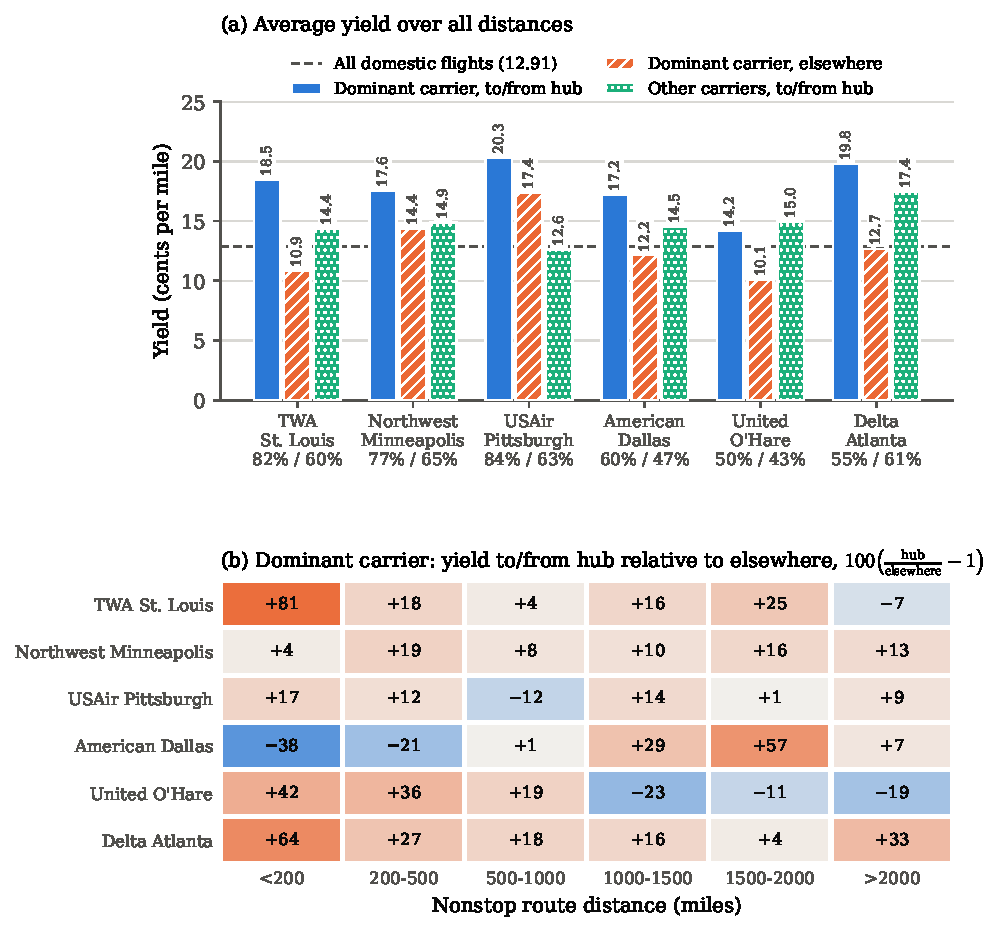
\includegraphics[width=0.97\linewidth]{figures/ch09/borenstein_yields.pdf}
\caption{Yields at six airports dominated by one carrier, third quarter of 1987. Panel (a) shows three yields
over all distances. They are the dominant carrier's yield on routes to or from its hub, its yield elsewhere in
its system, and the yield of other carriers on routes to or from the hub. The two percentages under each airport are the
dominant carrier's shares of enplanements and of originations there. Panel (b) shows, for each distance band,
the percentage by which the dominant carrier's yield to or from its hub exceeds its yield elsewhere. Yields fall
with distance, so panel (a) mixes fare levels with the distance composition of each group, while panel (b)
holds distance roughly fixed. Redrawn from \citet{Borenstein1989}, Table 1.}
\label{fig:09-bor-yields}
\end{figure}

Over all distances, the dominant carrier's yield at its hub exceeds its yield elsewhere at all six airports.
The gap ranges from 17\% for USAir at Pittsburgh ($\frac{20.32}{17.42} = 1.17$) to 70\% for TWA at St.\ Louis
($\frac{18.50}{10.86} = 1.70$). At five of the six airports, the dominant carrier's yield also exceeds that of
other carriers at the same airport. The exception is O'Hare, the least dominated airport in the table. There
United's yield of 14.19 cents falls short of the other carriers' 14.99 cents.

The comparison over all distances has a weakness. Yields fall steeply with distance, from 37.96 cents per mile
on routes under 200 miles to 7.16 cents on routes over 2,000 miles. A group that flies shorter routes therefore
shows a higher average yield even if it charges the same fare as others at each distance. Panel (b) of
\cref{fig:09-bor-yields} compares the dominant carrier with itself within distance bands. Its hub yield exceeds
its yield elsewhere in 29 of the 36 cells. The exceptions are Dallas on short routes ($-38\%$ and $-21\%$)
and O'Hare on routes over 1,000 miles ($-23\%$, $-11\%$ and $-19\%$). The others are Pittsburgh at 500 to
1,000 miles ($-12\%$) and St.\ Louis over 2,000 miles ($-7\%$). Against other carriers at the same airport, the dominant carrier has the
higher yield in 26 of the 35 cells with data. United at O'Hare is lower in five of six bands. USAir's 61\%
advantage over other carriers at Pittsburgh over all distances shrinks to between $-16\%$ and $+27\%$ within
bands, so most of it reflects the distance mix.\footnote{The within-band counts and percentages are our
calculations from Table 1 of the paper.}%

Borenstein argues that costs do not explain the hub premium (p.~356). Carriers have somewhat higher load
factors on flights to and from their hubs, which lowers cost per passenger. Passengers to or from a hub also
fly routes about as long as, or longer than, the carrier's other passengers. The higher cost per mile of short
flights therefore does not explain the gap either. The table cannot separate airport dominance from route
dominance, because a carrier that dominates an airport usually dominates the routes from it. The regressions
attempt this separation.

\subsection{The estimating equations}\label{sec:09-bor-equations}

\casehead{The pricing equation} Borenstein's first equation explains the log of a fare percentile by cost,
quality and market-structure variables. Let $P_{ft}$ denote one of FR20, FR50 or FR80 for carrier $f$ on route
$t$. Each percentile has its own regression with its own coefficients. In our notation, his equation (1), with
an error term $u_{ft}$ added, is
\begin{equation}\label{eq:09-bor-price}
\begin{aligned}
\ln P_{ft} = {} & a_f + b_D \ln \mathit{DISTANCE}_t + \gamma_1 \ln \mathit{LOADFAC}_{ft}
  + \gamma_2 \ln \mathit{EQUIP}_{ft} \\
& + \gamma_3 \ln \mathit{FREQ}_{ft} + \gamma_4 \ln \mathit{CIRC}_{ft} + \gamma_5\, \mathit{STOP}_{ft}
  + \gamma_6\, \mathit{PLANECHG}_{ft} \\
& + \phi_1\, \mathit{ORGSHARE}_{ft} + \phi_2\, \mathit{ORGHERF}_t + \phi_3\, \mathit{RUTSHARE}_{ft}
  + \phi_4\, \mathit{RUTHERF}_t \\
& + \phi_5 \ln \mathit{COMPCOST}_{ft} + \phi_6 \ln \mathit{TOURIST}_t
  + \sum_{k=1}^{24} \varrho_k\, \mathit{APT}_{kt} + u_{ft} .
\end{aligned}
\end{equation}
The coefficient letters group the variables by their hypothesized role (p.~349). The carrier effects $a_f$
capture carrier-wide differences in cost and reputation. Distance, with coefficient $b_D$, primarily affects
production cost. The six $\gamma$ variables affect both cost and service quality, so their signs are ambiguous
in advance. The six $\phi$ variables primarily indicate market power. The 24 coefficients $\varrho_k$ measure
scarcity rents at airports that may be congested. \Cref{tab:09-bor-vars} defines each variable and gives the
sign that Borenstein expects.

\begin{table}[htbp]
\centering
\caption{Variables of the pricing equation}
\label{tab:09-bor-vars}
\footnotesize
\renewcommand{\arraystretch}{1.12}
\begin{tabularx}{\linewidth}{@{}l >{\raggedright\arraybackslash}X l c@{}}
\toprule
Variable & Definition and construction & Group & Sign \\
\midrule
FR20, FR50, FR80 & Percentiles of the passenger-weighted distribution of the fares paid to the carrier on the
route. A round trip counts as two trips at half fare. & dependent & \\
DISTANCE & Nonstop mileage between the endpoints ($d_t$ in \cref{sec:09-data}). & cost & $+$ \\
LOADFAC & Load factor of the segments used by the carrier's passengers on the route, averaged over the
segments of an itinerary by distance and over itineraries by passengers. & cost, quality & ? \\
EQUIP & Seats per plane, averaged in the same way. & cost, quality & ? \\
FREQ & Minimum number of flights in the quarter on any segment of an itinerary, averaged over itineraries by
passengers. & cost, quality & ? \\
CIRC & Average total routing mileage of the carrier's passengers (TOTMILE) divided by DISTANCE. & cost, quality
& ? \\
STOP & Average number of on-plane stops per passenger. & cost, quality & ? \\
PLANECHG & Average number of changes of plane per passenger. & cost, quality & ? \\
ORGSHARE & Carrier's share of passenger originations at the two endpoints, averaged with weights equal to the
shares of the route's travelers whose tickets originate at each endpoint. & market power & $+$ \\
ORGHERF & Herfindahl index of originations at the two endpoints, averaged with the same weights. & market power
& ? \\
RUTSHARE & Carrier's share of the route's local passengers. & market power & $+$ \\
RUTHERF & Herfindahl index of the route's local passengers. & market power & ? \\
COMPCOST & Average standardized cost per available seat-mile of the other carriers on the route, weighted by
their route shares. & market power & $+$ \\
TOURIST & Tourism index (hotel income from group and tourist customers over personal income) of each endpoint,
weighted by the share of travelers who originate at the other endpoint. & market power & $-$ \\
APT$_k$ & Indicator that airport $k$ is an endpoint, divided by DISTANCE in thousands of miles. & scarcity &
$+$ \\
\bottomrule
\end{tabularx}

\smallskip
\begin{minipage}{\linewidth}
\footnotesize Notes: ``Group'' is the role that Borenstein assigns to each variable and ``Sign'' the sign he
expects, with ? for an ambiguous sign. Load factor, equipment, frequency and stops come from the Service
Segment Data, fares, shares and circuity from the DB1A sample, and enplanements from the Nonstop Market Data.
Source: \citet{Borenstein1989}, pp.~349--351 and Appendix.
\end{minipage}
\end{table}

\casehead{Constructed variables} Several variables are averages over the two endpoints $e \in \{1,2\}$ of the
route. Let $\varpi_{te}$ be the share of the route's travelers whose tickets originate at endpoint $e$. Let
$o_{fe}$ be carrier $f$'s share of all passenger originations at airport $e$, and let $\mathit{TRIX}_e$ be the
tourism index of the metropolitan area of $e$. Then
\begin{equation}\label{eq:09-bor-org}
\begin{gathered}
\mathit{ORGSHARE}_{ft} = \sum_{e=1}^{2} \varpi_{te}\, o_{fe}, \qquad
\mathit{ORGHERF}_t = \sum_{e=1}^{2} \varpi_{te} \sum_{k} o_{ke}^2, \\
\mathit{TOURIST}_t = \varpi_{t1}\, \mathit{TRIX}_2 + \varpi_{t2}\, \mathit{TRIX}_1 .
\end{gathered}
\end{equation}
The tourism measure weights each endpoint by the share of travelers who start at the other end, so it measures
the tourist appeal of the route's destinations. Origination shares exclude connecting passengers. Borenstein
reports that measures based on enplanements, which include them, give very similar results (p.~349).

The cost of rivals enters through
\begin{equation}\label{eq:09-bor-compcost}
\mathit{COMPCOST}_{ft} = \sum_{k \neq f} \frac{s_{kt}}{1 - s_{ft}}\, \mathit{COST}_k ,
\end{equation}
where $s_{kt}$ is carrier $k$'s route share, so that $s_{ft} = \mathit{RUTSHARE}_{ft}$. $\mathit{COST}_k$ is a
standardized cost per available seat-mile. To construct it, Borenstein regresses cost per available seat-mile on
a constant and average length of haul across the 17 carriers with data. He then adds each carrier's residual to
0.08, roughly the average cost of a carrier with the mean length of haul (p.~363). Small carriers without data
receive 0.08. COMPCOST proxies for the competitiveness of rivals, whose prices are endogenous and whose service
data are incomplete (p.~351).

Finally, the scarcity variables are
\begin{equation}\label{eq:09-bor-apt}
\mathit{APT}_{kt} = \frac{1000 \cdot \indic\{k \text{ is an endpoint of } t\}}{\mathit{DISTANCE}_t} ,
\end{equation}
for 24 airports (p.~351). They are the 22 airports that the Federal Aviation Administration monitored for
congestion and the airports of Orange County and Long Beach, which faced strict local limits on takeoffs and
landings. Four of the monitored airports allocated slots: O'Hare, Kennedy, La Guardia and Washington National.

\casehead{Expected signs} The $\gamma$ variables move cost and quality in directions that push price opposite
ways (pp.~349--350). A higher load factor lowers cost per passenger, which lowers fares. Full flights also tend
to operate at peak times, when the opportunity cost of aircraft is high, which raises fares. Crowded planes,
finally, lower service quality and reservation prices. Larger aircraft have a lower cost per seat-mile on
flights over 500 miles. They are also more comfortable and thought to be safer, which raises demand. Frequent
service lowers cost per flight, because aircraft on dense routes fly more hours per day. It also lowers the
frequency delay of \cref{sec:09-regulation}, the gap between a traveler's preferred departure time and the
nearest flight \citep{DouglasMiller1974}. Frequency delay matters most to travelers with high time values, who pay the high
fares. Circuity, stops and changes of plane raise cost, by lengthening routings or shortening average hauls,
and they lower quality.

Among the $\phi$ variables, Borenstein expects ORGSHARE, RUTSHARE and COMPCOST to raise fares and TOURIST to
lower them (pp.~350--351). The concentration measures have ambiguous signs, and their interpretation drives the
paper. Holding the carrier's own route share fixed, a higher RUTHERF means that the traffic the carrier does not
carry is more concentrated. If a dominant carrier's high price creates an umbrella, this raises the observed
carrier's price, so $\phi_4 > 0$. If a dominant carrier instead has a competitive advantage through marketing
devices, it may lower the profit-maximizing price of its rivals, so $\phi_4 < 0$. Endpoint concentration is
ambiguous for a related reason. A carrier may prefer many small rivals at its airports to one large rival,
while coordination, such as an agreement not to enter one another's routes, is easier among few firms.

\casehead{Functional form} A firm with market power sets price equal to marginal cost times a markup that
depends on the elasticity of the demand it faces. Logs turn this product into a sum, and earlier studies used
the same multiplicative form \citep{GrahamKaplanSibley1983,BaileyGrahamKaplan1985}. Most variables therefore
enter in logs, with constant elasticities. \Cref{sec:09-pricing-conduct} derives this specification from a
model of conduct. Let collusiveness rise with concentration as $\eta_t = \eta_0 + \eta_1 \HHI_t$, and let the
elasticity be a common $\varepsilon$. Because the equation omits the interaction $\HHI_t s_{ft}$ of
\cref{eq:09-umbrella}, the route-share coefficient is then $\phi_3 \approx \frac{1 - \eta_0 - \eta_1 \bar H}{\varepsilon}$
and the route-Herfindahl coefficient is $\phi_4 \approx \frac{\eta_1 (1 - \bar s)}{\varepsilon}$. Here $\bar H$
and $\bar s$ are the sample means of RUTHERF and RUTSHARE. The cost and quality variables parametrize
$\ln mc_{ft}$, and the constant terms are absorbed by the carrier effects.

The theory thus implies that shares enter linearly, and Borenstein gives a direct argument for the same choice
(p.~354). A log specification would give a rise in share from 1\% to 2\% the same effect as a rise from 30\% to
60\%, which is implausible. ORGSHARE enters linearly for the same reason, and
the two Herfindahl indices enter linearly for ease of comparison. The signs and approximate significance of
the estimates are robust to logs for each of these variables. STOP and PLANECHG also enter linearly, so each
stop or change of plane has the same proportional effect on price.

\Cref{rem:09-share-coef} shows that a Cournot reading of the 2SLS share coefficients ($\bar\eta = 0$, so
$\varepsilon = \frac{1}{\phi_3}$) would require route elasticities of $\frac{1}{0.1120} = 8.9$,
$\frac{1}{0.0288} = 34.7$ and $\frac{1}{0.2238} = 4.5$ for the three percentiles. The variation across
percentiles adds a further difficulty. A homogeneous-goods model has one price per route, and hence one
elasticity for all fares, while the share coefficients differ nearly eightfold across percentiles. Each
percentile behaves as if it faced its own demand. A model with differentiated products and heterogeneous
travelers delivers this pattern (\cref{sec:09-pricing-types}).

The scarcity terms need a different treatment (p.~354). A scarcity rent should add the same dollar amount to
every fare from an airport, whatever the route. Suppose the fare is $P_{ft} = P^0_{ft} + R_k$, where $P^0_{ft}$
is the fare without the rent and $R_k$ is the rent at endpoint $k$. Taking logs and using
$\ln(1 + x) \approx x$ for small $x$,
\begin{align*}
\ln P_{ft} &= \ln P^0_{ft} + \ln\left(1 + \frac{R_k}{P^0_{ft}}\right) \\
&\approx \ln P^0_{ft} + \frac{R_k}{P^0_{ft}} .
\end{align*}
If the rent-free fare is proportional to distance, $P^0_{ft} = c\, \mathit{DISTANCE}_t$, the last term becomes
\begin{equation*}
\frac{R_k}{c\, \mathit{DISTANCE}_t} = \frac{R_k}{1000\, c} \cdot \frac{1000}{\mathit{DISTANCE}_t}
= \varrho_k\, \mathit{APT}_{kt}, \qquad \text{with } \varrho_k = \frac{R_k}{1000\, c} .
\end{equation*}
The coefficient $\varrho_k$ is thus the rent as a fraction of the fare on a 1,000-mile route. A plain indicator
would instead make the rent proportional to the fare and assign larger rents to longer routes. Estimating the
additive form directly would require iterative nonlinear methods, which would have been difficult with his
number of observations and variables. Borenstein therefore calls the distance scaling a partial solution. Fares
rise less than proportionally with distance ($b_D$ lies between 0.33 and 0.41 in \cref{tab:09-bor-main}), so
dividing by distance overcorrects somewhat.

\casehead{The relative-price equation} The second equation compares two carriers on the same route. Add to
\cref{eq:09-bor-price} a route effect $\Upsilon_t$ that collects every determinant of fares common to all carriers
on route $t$, observed or not. Collect the variables that vary across carriers on a route in the row vector
\begin{equation*}
z_{ft} = \big(\ln \mathit{LOADFAC}_{ft}, \ln \mathit{EQUIP}_{ft}, \ln \mathit{FREQ}_{ft}, \ln \mathit{CIRC}_{ft},
\mathit{STOP}_{ft}, \mathit{PLANECHG}_{ft}\big),
\end{equation*}
with coefficients $\gamma = (\gamma_1, \dots, \gamma_6)^\top$. The pricing equation becomes
\begin{equation*}
\ln P_{ft} = a_f + \Upsilon_t + z_{ft}\gamma + \phi_1\, \mathit{ORGSHARE}_{ft} + \phi_3\, \mathit{RUTSHARE}_{ft}
+ \phi_5 \ln \mathit{COMPCOST}_{ft} + u_{ft} .
\end{equation*}
Here $\Upsilon_t$ absorbs distance, the two Herfindahl indices, the tourism index, the scarcity terms and any
unobserved demand or cost shifter at the route level. Write this equation for carriers $a$ and $b$ on route $t$
and subtract. The route effect cancels because $\Upsilon_t - \Upsilon_t = 0$. Borenstein also omits the difference in
COMPCOST (p.~355, n.~35). Its role in the pricing equation was to proxy for the other carriers on the route. In
the relative-price equation one rival enters directly and the remaining rivals are common to both carriers. The
result is his equation (4):
\begin{equation}\label{eq:09-bor-rel}
\begin{aligned}
\ln P_{at} - \ln P_{bt} = {} & a_a - a_b + \gamma_1 (\ln \mathit{LOADFAC}_{at} - \ln \mathit{LOADFAC}_{bt}) \\
& + \gamma_2 (\ln \mathit{EQUIP}_{at} - \ln \mathit{EQUIP}_{bt})
  + \gamma_3 (\ln \mathit{FREQ}_{at} - \ln \mathit{FREQ}_{bt}) \\
& + \gamma_4 (\ln \mathit{CIRC}_{at} - \ln \mathit{CIRC}_{bt})
  + \gamma_5 (\mathit{STOP}_{at} - \mathit{STOP}_{bt}) \\
& + \gamma_6 (\mathit{PLANECHG}_{at} - \mathit{PLANECHG}_{bt})
  + \phi_1 (\mathit{ORGSHARE}_{at} - \mathit{ORGSHARE}_{bt}) \\
& + \phi_3 (\mathit{RUTSHARE}_{at} - \mathit{RUTSHARE}_{bt}) + u_{at} - u_{bt} .
\end{aligned}
\end{equation}
The coefficients are those of \cref{eq:09-bor-price}. The two carriers are drawn at random among those that meet
the sample criteria (p.~355). The carrier effects enter as the difference $a_a - a_b$, which a regression
implements with indicators equal to $+1$ for carrier $a$ and $-1$ for carrier $b$.

Differencing has a benefit and a cost. The benefit is that every unobserved route-level shifter of demand or
cost drops out. The estimates of $\phi_1$ and $\phi_3$ then no longer rely on the route controls of
\cref{eq:09-bor-price}. The cost is that the coefficients on route-level market structure, $\phi_2$ and
$\phi_4$, are no longer identified. The equation answers a narrower question, which is the one the asymmetry
hypothesis poses. Does the carrier with the larger share of a route, or of its endpoints, charge more than its
rival on the same route? Under a complete umbrella with a homogeneous product, $\eta_t = 1$ and every carrier on
the route has conduct $\theta_{ft} = 1$. The share term in \cref{eq:09-pricing-approx} then vanishes, and all
carriers charge the same markup, so $\phi_3 = 0$ in \cref{eq:09-bor-rel}. Under the differentiated-products
model of \cref{prop:09-dominance}, the relative price instead rises with the share gap. Let $s$ be a common
share of all potential travelers, $L$ the Lerner index there and $s_0$ the outside share. \Cref{cor:09-relprice}
gives a slope of $\frac{L}{1-s}$ in these shares, or $\frac{L(1-s_0)}{1-s}$ in route shares. The latter is
the structural counterpart of $\phi_3$ in \cref{eq:09-bor-rel}.

\subsection{Estimation and identification}\label{sec:09-bor-ident}

\casehead{Why least squares fails} A carrier's route share depends on its own price. To see the consequence,
add a share equation to the pricing equation and solve the two jointly. Suppress the other regressors, which
we take as exogenous, and write
\begin{align*}
\ln P_{ft} &= \phi_3\, s_{ft} + u_{ft}, \\
s_{ft} &= \Psi_{ft} - b_s \ln P_{ft} + v_{ft} .
\end{align*}
Here $s_{ft} = \mathit{RUTSHARE}_{ft}$, $\Psi_{ft}$ collects exogenous shifters of the share, $b_s > 0$
measures how fast the share falls with the carrier's own price, and $v_{ft}$ is an unobserved demand shifter.
Substitute the first equation into the second:
\begin{equation*}
s_{ft} = \Psi_{ft} - b_s \phi_3\, s_{ft} - b_s u_{ft} + v_{ft} .
\end{equation*}
Collect the terms in $s_{ft}$ and solve, assuming $1 + b_s \phi_3 > 0$:
\begin{equation*}
s_{ft} = \frac{\Psi_{ft} - b_s u_{ft} + v_{ft}}{1 + b_s \phi_3} .
\end{equation*}
Let $\Var(u_{ft}) = \sigma_u^2$ and $\Cov(u_{ft}, v_{ft}) = \sigma_{uv}$, and let $\Psi_{ft}$ be uncorrelated
with both errors. The ordinary least squares (OLS) estimator then has probability limit
\begin{equation}\label{eq:09-bor-olsbias}
\plim \hat\phi_3^{\mathrm{OLS}} = \phi_3 + \frac{\Cov(s_{ft}, u_{ft})}{\Var(s_{ft})}
= \phi_3 + \frac{\sigma_{uv} - b_s \sigma_u^2}{(1 + b_s\phi_3) \Var(s_{ft})} .
\end{equation}
With other regressors present, $\Var(s_{ft})$ is the variance of the share after projection on them. Two forces
compete. The simultaneity term $-b_s\sigma_u^2$ biases the estimate down. A carrier hit by a positive cost
or pricing shock charges more and loses passengers, so high prices go with low shares. The term $\sigma_{uv}$
biases the estimate up if unobserved quality raises both the share and the price, which is the efficiency
argument of \citet{Demsetz1973} in airline form. A Hausman test (described below) rejects the exogeneity of
RUTSHARE and RUTHERF (p.~352), so the preferred estimates use instruments.

\casehead{The instrument for route share} An instrument must shift a carrier's route share without entering its
pricing equation. Measures of rivals' presence at the endpoint airports come to mind. The airport dominance
effects of \cref{sec:09-dominance-sources}, however, make such measures candidates for the pricing equation
itself (p.~352). Borenstein resolves the problem with an asymmetry. The marketing advantages of airport
dominance do not require large operations at both ends of a route. Entry onto a route, in contrast, benefits
from presence at both ends. The excluded instrument is the carrier's share of the geometric means of endpoint
enplanements,
\begin{equation}\label{eq:09-genpsh}
\mathit{GENPSH}_{ft} = \frac{\sqrt{\mathit{ENP}_{f1}\, \mathit{ENP}_{f2}}}
{\sum_{k} \sqrt{\mathit{ENP}_{k1}\, \mathit{ENP}_{k2}}} ,
\end{equation}
which is his equation (2). Here $\mathit{ENP}_{k1}$ and $\mathit{ENP}_{k2}$ are carrier $k$'s average daily
enplanements at the two endpoints of route $t$ during the quarter, and the sum runs over all carriers
(p.~352).

The geometric mean gives the instrument its content. It is zero when a carrier has no enplanements at one of
the endpoints. For a given total $\mathit{ENP}_{f1} + \mathit{ENP}_{f2}$, it is largest when the two are equal.
GENPSH therefore rewards balanced presence at both ends. ORGSHARE, which appears in the pricing equation,
averages the carrier's endpoint shares linearly. A carrier with a large share at one end and a small share at
the other can have a high ORGSHARE but a low GENPSH. Conditional on ORGSHARE, GENPSH thus varies with the
balance of the carrier's presence across the endpoints. It also varies with connecting operations, since
enplanements count connecting passengers and originations do not. Borenstein chooses enplanements because they
better measure a carrier's investment in physical capital and long-term labor contracts at an airport
(p.~352, n.~30).

Two pieces of evidence support relevance. The first comes from \citet{Berry1992}, which Borenstein cites as a
1989 working paper (p.~352, n.~29). Berry starts from the 1,225 possible city pairs among the 50 largest U.S.
cities \citep[p.~903]{Berry1992}. He drops 6 pairs that have no listings in the Origin and Destination Survey,
which leaves 1,219 markets \citep[p.~903, n.~9, and p.~904]{Berry1992}. He measures entry between the first and the third quarter of 1980
\citep[p.~904]{Berry1992}. Of the 3,590
potential entrants that already served both cities of a pair, 6.46\% entered it. Of those that served one city,
0.36\% entered, a rate about 18 times lower. Only 4 of the 47,600 potential entrants that served neither city entered,
a rate of 0.01\% \citep[Table~III]{Berry1992}. The second piece of evidence is Borenstein's own. In the first
stage of the estimation, both ORGSHARE and GENPSH are highly significant (p.~352). The paper does not report the first-stage coefficients or $F$ statistics.

The exclusion restriction requires that GENPSH affect fares only through route share. Borenstein states the
condition plainly. It is valid if a carrier's current prices respond to actual competition but not to threats
of entry (p.~352). He defends it on timing grounds. An incumbent can change its fares much faster than a rival
can move from announcing entry to flying. It therefore need not price against potential entrants in advance. The USAir testimony quoted in \cref{sec:09-contest-fail} supports this view.

If the restriction fails, the bias has a predictable sign. Potential entrants with large operations at both
endpoints raise the denominator of \cref{eq:09-genpsh}, so a carrier's GENPSH is low exactly when such entrants
are present. Suppose a carrier that faces well-placed potential entrants holds its fares down to deter entry, a
practice called \emph{limit pricing}. Its fares then rise with GENPSH at a given route share, and the true
equation contains a term $\phi_G\, \mathit{GENPSH}_{ft}$ with $\phi_G > 0$. Ignore RUTHERF for the moment, write $g_{ft} = \mathit{GENPSH}_{ft}$, and let a tilde denote the
residual after projection on the included exogenous regressors. The IV estimator has probability limit
\begin{align}
\plim \hat\phi_3^{\mathrm{IV}} &= \frac{\Cov(\tilde g_{ft}, \ln P_{ft})}{\Cov(\tilde g_{ft}, \tilde s_{ft})}
\notag \\
&= \frac{\phi_3 \Cov(\tilde g_{ft}, \tilde s_{ft}) + \phi_G \Var(\tilde g_{ft})}{\Cov(\tilde g_{ft}, \tilde s_{ft})}
\notag \\
&= \phi_3 + \frac{\phi_G}{\pi_1} . \label{eq:09-bor-ivbias}
\end{align}
The second line substitutes the true equation and uses $\Cov(\tilde g_{ft}, u_{ft}) = 0$. In the third line,
$\pi_1 = \frac{\Cov(\tilde g_{ft}, \tilde s_{ft})}{\Var(\tilde g_{ft})}$ is the first-stage coefficient on
GENPSH. Since $\pi_1 > 0$ and $\phi_G > 0$, limit pricing against potential entrants biases the estimated
share effect upward. A violation of this kind would make Borenstein's estimates of $\phi_3$ too large. The
POTCOMP specification below offers a check. Controlling for potential competitors should absorb part of this
bias and lower the route-share coefficients. Instead they rise slightly (Panel B of \cref{tab:09-bor-main}),
which suggests that the bias is small.

\casehead{Potential competition} Borenstein addresses the exclusion restriction in a second way, by measuring
potential competition directly (pp.~352--353). The variable
\begin{equation}\label{eq:09-bor-potcomp}
\mathit{POTCOMP}_{ft} = \frac{\sum_{k \in \mathcal{P}_t} \sqrt{\mathit{ENP}_{k1}\, \mathit{ENP}_{k2}}}
{\sum_{k} \sqrt{\mathit{ENP}_{k1}\, \mathit{ENP}_{k2}}}
\end{equation}
has the construction of GENPSH, but its numerator sums over the set $\mathcal{P}_t$ of carriers with less than
1\% of the route's traffic (p.~364). These carriers are present at the endpoints but not yet significant on the
route. In an alternative specification POTCOMP enters \cref{eq:09-bor-price} directly, while GENPSH still
instruments route share. POTCOMP may itself be endogenous. High fares on a route attract entry, which turns
potential competitors into actual ones and lowers POTCOMP. A positive shock $u_{ft}$ therefore goes with a low
POTCOMP, which biases its coefficient toward a negative value (p.~359, n.~44).

\casehead{The instrument for route concentration} The route Herfindahl index contains the square of the
carrier's own share, so it is endogenous whenever RUTSHARE is. Borenstein constructs an instrument by
decomposing the index (p.~353). Write $s_{ft}$ for the carrier's share and $\HHI_t = \mathit{RUTHERF}_t$. Split
the sum of squared shares into the carrier's own term and its rivals' terms:
\begin{align*}
\HHI_t &= s_{ft}^2 + \sum_{k \neq f} s_{kt}^2 \\
&= s_{ft}^2 + (1 - s_{ft})^2 \sum_{k \neq f} \left(\frac{s_{kt}}{1 - s_{ft}}\right)^2 \\
&= s_{ft}^2 + (1 - s_{ft})^2 H_{-f,t} .
\end{align*}
Here $H_{-f,t}$ is the Herfindahl index of the traffic that carrier $f$ does not carry, computed from each
rival's share of that traffic. Solving the last line for $H_{-f,t}$ expresses it in observed variables:
\begin{equation*}
H_{-f,t} = \frac{\mathit{RUTHERF}_t - \mathit{RUTSHARE}_{ft}^2}{(1 - \mathit{RUTSHARE}_{ft})^2} .
\end{equation*}

The instrument rests on two assumptions. (a) GENPSH is a valid instrument for RUTSHARE. (b) The division among
rivals of the traffic that carrier $f$ does not carry is exogenous to $f$'s price. In Borenstein's example,
TWA's price on the Boston to Los Angeles route does not affect how the passengers it does not get divide between
American and United. Under (b), $H_{-f,t}$ is exogenous. Replace the own share by its fitted value
$\widehat{\mathit{RUTSHARE}}_{ft}$ from the first-stage regression on all exogenous variables:
\begin{equation}\label{eq:09-irutherf}
\mathit{IRUTHERF}_{ft} = \widehat{\mathit{RUTSHARE}}_{ft}^{\,2}
+ \frac{\mathit{RUTHERF}_t - \mathit{RUTSHARE}_{ft}^2}{(1 - \mathit{RUTSHARE}_{ft})^2}
\big(1 - \widehat{\mathit{RUTSHARE}}_{ft}\big)^2 .
\end{equation}
This is Borenstein's equation (3). In the constructed index, each rival's share becomes
$s_{kt} \frac{1 - \widehat{\mathit{RUTSHARE}}_{ft}}{1 - s_{ft}}$. The rescaling leaves the Herfindahl index of the
traffic not carried by $f$ equal to $H_{-f,t}$, as Borenstein notes. IRUTHERF then serves as the excluded
instrument for RUTHERF. The same assumption (b) is needed for COMPCOST, whose weights in
\cref{eq:09-bor-compcost} are the rivals' shares of the traffic that $f$ does not carry (p.~353).

\begin{remark}[When is assumption (b) plausible?]\label{rem:09-bor-iia}
Assumption (b) holds exactly in a logit model of route demand, holding rivals' prices fixed. Route shares are
shares of the route's passengers, so the outside good drops out and
$s_{kt} = \frac{e^{\delta_{kt}}}{\sum_{j} e^{\delta_{jt}}}$, with the sum over the carriers on the route. Then
\begin{equation*}
\frac{s_{kt}}{1 - s_{ft}} = \frac{e^{\delta_{kt}}}{\sum_{j \neq f} e^{\delta_{jt}}} ,
\end{equation*}
which involves neither $\delta_{ft}$ nor $p_{ft}$. This is the independence of irrelevant alternatives of
\cref{ch:logit}. The assumption fails when some rivals are closer substitutes for $f$ than others, for example
when one rival shares $f$'s hub airport. It can also fail in equilibrium, since rivals adjust their prices when
$f$ changes its own.
\end{remark}

\begin{remark}[A constructed instrument]\label{rem:09-bor-generated}
IRUTHERF is a nonlinear function of first-stage fitted values. Substituting such a function for RUTHERF in the
second stage would not in general give consistent estimates, because the first-stage residual does not drop out
of a nonlinear function. Borenstein instead uses IRUTHERF as an excluded instrument in the first-stage regression
for RUTHERF. Any function of exogenous variables is a valid instrument, so this use is consistent under (a) and
(b). The nonlinearity affects only how strongly IRUTHERF predicts RUTHERF.
\end{remark}

\casehead{Load factor and the Hausman test} Load factor may also be endogenous, since a low fare fills planes.
Borenstein instruments it with LOADPOP, the passenger-weighted average over itineraries of the summed
populations of all cities where the traveler is on the ground, including stops and connections (pp.~353, 363).
The idea is that populous cities along an itinerary add traffic to its segments and so raise load factors. A
Hausman test does not reject exogeneity of LOADFAC at any reasonable significance level, so the reported
estimates treat it as exogenous (pp.~356--357).

The Hausman test compares two estimators \citep{Hausman1978}. Under the null hypothesis that the suspect
regressors are exogenous, OLS is consistent and efficient, while 2SLS is consistent but less precise. Under the
alternative only 2SLS is consistent. Let $\hat\vartheta_S$ collect the estimated coefficients on the suspect
regressors and $\hat V$ their estimated variance matrix. The statistic
\begin{equation}\label{eq:09-bor-hausman}
\mathcal{H} = \big(\hat\vartheta_S^{\mathrm{2SLS}} - \hat\vartheta_S^{\mathrm{OLS}}\big)^\top
\big[\hat V^{\mathrm{2SLS}} - \hat V^{\mathrm{OLS}}\big]^{-1}
\big(\hat\vartheta_S^{\mathrm{2SLS}} - \hat\vartheta_S^{\mathrm{OLS}}\big)
\end{equation}
is asymptotically $\chi^2$ under the null, with degrees of freedom equal to the number of suspect regressors
(\cref{sec:A-spectests}). A large value rejects exogeneity. For RUTSHARE and RUTHERF the test rejects, and
for LOADFAC it does not.

Treating LOADFAC as endogenous anyway raises the estimated ORGSHARE effects somewhat and raises all standard
errors (p.~357, n.~38). The LOADFAC coefficient itself becomes much more negative and much less precise
(p.~358, n.~40). Simultaneity predicts the opposite movement. Low fares raise load factors, which pushes the
least-squares coefficient down, so a correction should make it less negative.

\casehead{Variables without instruments} A carrier's choices of nonstop versus connecting service, aircraft
size, frequency, stops, changes of plane and circuity are part of its network design. They may respond to the
same shocks as its fares (p.~353). Even LOADPOP is open to doubt, since the populations are exogenous but their
summation by itinerary depends on routing choices. For lack of instruments, Borenstein treats these variables as
exogenous and interprets their coefficients with possible biases in mind.

\casehead{Pooling and the error structure} A test rejects a common constant across carriers, so the equation
includes carrier fixed effects $a_f$ (pp.~353--354). A further test of common slopes across carriers does not
reject pooling at conventional levels, so all other coefficients are common to the nine carriers. The
scarcity coefficients $\varrho_k$ are common by construction, since a scarcity rent is the same for every
carrier at an airport. The same tests applied to \cref{eq:09-bor-rel} again do not reject pooling (p.~355).
Keeping one carrier per route gives up information to secure independent errors. A modern study would keep
every qualifying carrier and cluster the standard errors by route (\cref{sec:A-cluster}).

\casehead{The estimator} The preferred estimates are 2SLS with asymptotic standard errors. The procedure has
three steps. First, regress RUTSHARE on GENPSH and all included exogenous regressors, and keep the fitted
values. Second, construct IRUTHERF from \cref{eq:09-irutherf}. Third, estimate \cref{eq:09-bor-price} by 2SLS,
treating RUTSHARE and RUTHERF as endogenous, with GENPSH and IRUTHERF as excluded instruments. With two
endogenous regressors and two excluded instruments, the equation is exactly identified. Let $X_{ft}$ be the row
of regressors, let $Z_{ft}$ be the same row with GENPSH and IRUTHERF in place of RUTSHARE and RUTHERF, and let
$\vartheta$ be the coefficient vector. The estimator solves the sample analogue of
$\E[Z_{ft}^\top u_{ft}] = 0$,
\begin{equation*}
\hat\vartheta = \Big(\sum_{t} Z_{ft}^\top X_{ft}\Big)^{-1} \sum_{t} Z_{ft}^\top \ln P_{ft} ,
\end{equation*}
where each route $t$ contributes the one carrier $f$ selected for it. The paper treats the endogeneity in
\cref{eq:09-bor-rel} in the same way, without detailing the instrument for the share difference. OLS estimates
are reported for comparison.

\subsection{Results}\label{sec:09-bor-results}

\casehead{The pricing equation} \Cref{tab:09-bor-main} reproduces Table 2 of the paper. Panel A gives the 2SLS
estimates of \cref{eq:09-bor-price} for the three fare percentiles. Panel B gives the market-power coefficients
from two alternative specifications, one with POTCOMP added and one estimated by OLS. The paper summarizes the
carrier effects and the scarcity coefficients in the text without reporting them. \Cref{fig:09-bor-coefs} plots
the main market-power coefficients with 95\% confidence intervals.

\begin{table}[htbp]
\centering
\caption{The pricing equation: estimates of \cref{eq:09-bor-price}}
\label{tab:09-bor-main}
\footnotesize
\begin{tabular}{@{}lccc@{}}
\toprule
\multicolumn{4}{@{}l}{\textit{Panel A. 2SLS}} \\
\addlinespace
Dependent variable & $\ln$ FR20 & $\ln$ FR50 & $\ln$ FR80 \\
\midrule
$\ln$ DISTANCE & 0.4138$^{*}$ & 0.3348$^{*}$ & 0.3559$^{*}$ \\
 & (0.0103) & (0.0124) & (0.0133) \\
$\ln$ LOADFAC & $-0.0754^{*}$ & $-0.0425$ & $-0.0240$ \\
 & (0.0264) & (0.0318) & (0.0341) \\
$\ln$ EQUIP & $-0.0160$ & $-0.0050$ & $-0.0691^{*}$ \\
 & (0.0187) & (0.0225) & (0.0242) \\
$\ln$ FREQ & 0.0140$^{\#}$ & 0.0236$^{*}$ & 0.0428$^{*}$ \\
 & (0.0078) & (0.0094) & (0.0101) \\
$\ln$ CIRC & 0.1458$^{*}$ & 0.1272$^{*}$ & 0.2062$^{*}$ \\
 & (0.0412) & (0.0497) & (0.0533) \\
STOP & $-0.0470$ & $-0.0340$ & $-0.1327^{*}$ \\
 & (0.0292) & (0.0352) & (0.0377) \\
PLANECHG & $-0.0293^{*}$ & $-0.0776^{*}$ & $-0.0616^{*}$ \\
 & (0.0111) & (0.0134) & (0.0144) \\
ORGSHARE & 0.0345 & 0.1254$^{\#}$ & 0.1191$^{\#}$ \\
 & (0.0549) & (0.0661) & (0.0710) \\
ORGHERF & $-0.0699$ & $-0.0893$ & 0.0766 \\
 & (0.0623) & (0.0751) & (0.0806) \\
RUTSHARE & 0.1120$^{\#}$ & 0.0288 & 0.2238$^{*}$ \\
 & (0.0606) & (0.0731) & (0.0784) \\
RUTHERF & 0.1559$^{\dagger}$ & 0.1822$^{\dagger}$ & $-0.1787^{\dagger}$ \\
 & (0.0696) & (0.0839) & (0.0901) \\
$\ln$ COMPCOST & 0.5042$^{*}$ & 0.7010$^{*}$ & 0.8374$^{*}$ \\
 & (0.0453) & (0.0546) & (0.0586) \\
$\ln$ TOURIST & $-0.0187^{*}$ & $-0.0558^{*}$ & $-0.0991^{*}$ \\
 & (0.0058) & (0.0070) & (0.0076) \\
\addlinespace
$R^2$ & 0.683 & 0.494 & 0.508 \\
Observations & 3,591 & 3,591 & 3,591 \\
\bottomrule
\end{tabular}

\bigskip
\begin{tabular}{@{}lcccccc@{}}
\toprule
\multicolumn{7}{@{}l}{\textit{Panel B. Market-power coefficients in alternative specifications}} \\
\addlinespace
& \multicolumn{3}{c}{2SLS with POTCOMP} & \multicolumn{3}{c}{OLS} \\
\cmidrule(lr){2-4} \cmidrule(l){5-7}
Dependent variable & $\ln$ FR20 & $\ln$ FR50 & $\ln$ FR80 & $\ln$ FR20 & $\ln$ FR50 & $\ln$ FR80 \\
\midrule
ORGSHARE & 0.0365 & 0.1227$^{\#}$ & 0.1205$^{\#}$ & 0.0819$^{\#}$ & 0.1229$^{*}$ & 0.1228$^{\dagger}$ \\
 & (0.0536) & (0.0647) & (0.0696) & (0.0426) & (0.0514) & (0.0551) \\
ORGHERF & $-0.0684$ & $-0.0750$ & 0.0934 & $-0.0264$ & $-0.0660$ & $-0.0033$ \\
 & (0.0633) & (0.0764) & (0.0822) & (0.0543) & (0.0656) & (0.0702) \\
RUTSHARE & 0.1196$^{\dagger}$ & 0.0564 & 0.2470$^{*}$ & 0.0899$^{*}$ & 0.0596$^{\#}$ & 0.1259$^{*}$ \\
 & (0.0577) & (0.0697) & (0.0749) & (0.0270) & (0.0326) & (0.0349) \\
RUTHERF & 0.1262$^{\#}$ & 0.1286 & $-0.2302^{*}$ & 0.1128$^{*}$ & 0.1323$^{*}$ & $-0.0120$ \\
 & (0.0659) & (0.0795) & (0.0855) & (0.0329) & (0.0397) & (0.0425) \\
POTCOMP & $-0.0589^{\dagger}$ & $-0.0449$ & $-0.0380$ & & & \\
 & (0.0289) & (0.0348) & (0.0375) & & & \\
\addlinespace
$R^2$ & 0.683 & 0.493 & 0.507 & 0.683 & 0.494 & 0.511 \\
Observations & 3,591 & 3,591 & 3,591 & 3,591 & 3,591 & 3,591 \\
\bottomrule
\end{tabular}

\smallskip
\begin{minipage}{0.95\linewidth}
\footnotesize Notes: Standard errors in parentheses, asymptotic except for OLS. Significance marks as printed in
the paper: $^{\#}$ 10\%, $^{\dagger}$ 5\%, $^{*}$ 1\%. All specifications include carrier fixed effects and the 24
airport scarcity variables, whose coefficients the paper does not report. The two specifications in Panel B
include all the regressors of Panel A, and their other coefficients are close to those of Panel A. Source:
\citet{Borenstein1989}, Table 2.
\end{minipage}
\end{table}

\begin{figure}[htbp]
\centering
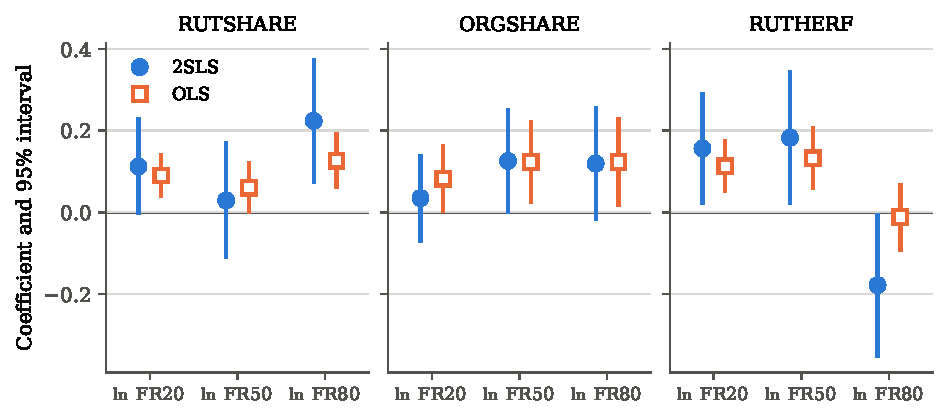
\includegraphics[width=0.97\linewidth]{figures/ch09/borenstein_coefs.pdf}
\caption{Market-power coefficients of the pricing equation by fare percentile, with 95\% confidence intervals
(estimate plus or minus 1.96 standard errors). Filled circles are 2SLS estimates and hollow squares OLS
estimates. The route-share and airport-share effects are positive at every percentile. The route-Herfindahl
effect, which holds the carrier's own share fixed, changes sign at the 80th percentile. Redrawn from
\citet{Borenstein1989}, Table 2.}
\label{fig:09-bor-coefs}
\end{figure}

Route share raises fares. Holding route concentration fixed, a one percentage point increase in a carrier's
route share raises its fares by between 0.03\% (FR50) and 0.22\% (FR80) (p.~357). Consider a dominant carrier
with 70\% of a route and rivals with 10\% each. All of them face the same route Herfindahl index, so the
comparison holds RUTHERF fixed automatically. The fare gap in log points is
\begin{equation*}
0.60 \times 0.1120 = 0.067, \qquad 0.60 \times 0.0288 = 0.017, \qquad 0.60 \times 0.2238 = 0.134
\end{equation*}
for FR20, FR50 and FR80. Borenstein summarizes this as a premium ``from 2\% to 12\%.''\footnote{The
arithmetic gives 1.7\% to 13.4\% in log points, or 1.7\% to 14.4\% as exact percentage changes
$e^{0.60\,\hat\phi_3} - 1$. The author's rounded range understates the upper end.} The effect is larger on the
20th and 80th percentiles than on the median, which Borenstein finds surprising. Yet a \emph{Chow test}, here a
test of whether a coefficient is equal across the three percentile regressions, does not reject equality
(p.~358). Only the FR80 coefficient is significant at 1\%. The FR20
coefficient is significant at 10\%, and the FR50 coefficient is not significant.

Airport share also raises fares, and more so at the high end of the fare distribution. The FR80 coefficient on
ORGSHARE, 0.1191, is about three times the FR20 coefficient, 0.0345, and Borenstein reports that the difference
is significant at 10\% (p.~358). Travelers who pay full coach fares are much more likely to be active members
of frequent-flyer programs than travelers on deep discounts. A stronger effect on high fares therefore fits the
FFP mechanism. A one standard deviation increase in ORGSHARE, 0.1305, raises the three log fares directly by
\begin{equation*}
0.1305 \times 0.0345 = 0.0045, \qquad 0.1305 \times 0.1254 = 0.0164, \qquad 0.1305 \times 0.1191 = 0.0155,
\end{equation*}
which the paper rounds to 0.5\%, 1.6\% and 1.6\%. Consider a carrier with half the originations at both
endpoints. It charges median and high-end fares about $0.5 \times 0.12 = 0.06$, or 6\%, above those of a
carrier with a very small presence at the two airports (p.~358).

These figures ignore an indirect channel. Airport dominance also raises a carrier's share of every route from
the airport. Borenstein estimates the size of this channel in a companion discussion paper, ``The Competitive
Advantage of a Dominant Airline'' (p.~358).\footnote{University of Michigan, Institute of Public Policy Studies,
Discussion Paper 280, 1989, as listed in the article's references. We cite it in the text only, so that its year
does not collide with the article's in the bibliography.} A one point increase in a carrier's share of originations at an airport raises its share of a route by up to 0.33
points, depending on its initial share. At the FR80 coefficient on route share, the indirect channel adds at most
$0.33 \times 0.2238 = 0.074$ to the direct ORGSHARE coefficient of 0.1191. When RUTSHARE and RUTHERF are dropped
from the equation, a one point increase in ORGSHARE raises the three percentiles by 0.24\%, 0.26\% and 0.24\%,
each significant at 1\% (p.~360, n.~46). These reduced-form effects exceed the sums of the direct and maximal
indirect effects implied by \cref{tab:09-bor-main}, which are 0.07, 0.13 and 0.19 per unit of
ORGSHARE.\footnote{The sums are $0.0345 + 0.33 \times 0.1120$, $0.1254 + 0.33 \times 0.0288$ and
$0.1191 + 0.33 \times 0.2238$. This comparison is our calculation.} By the omitted-variable formula, the
reduced-form coefficient picks up the full sample association of airport share with route share and route
concentration, which can exceed the causal channel.

Route concentration, holding the carrier's own share fixed, has mixed effects. It raises low-end and median fares
and lowers high-end fares, and all three coefficients are significant at 5\%. Borenstein illustrates with a
merger. Let firm 1 carry half of a route's passengers and two rivals a quarter each. A merger of the two rivals
changes the route Herfindahl index from
\begin{equation*}
0.5^2 + 2 \times 0.25^2 = 0.375 \qquad \text{to} \qquad 0.5^2 + 0.5^2 = 0.5,
\end{equation*}
an increase of 0.125, slightly more than half a standard deviation ($\frac{0.125}{0.2237} = 0.56$). Holding
firm 1's share fixed, its log fares change by
\begin{equation*}
0.125 \times 0.1559 = 0.019, \qquad 0.125 \times 0.1822 = 0.023, \qquad 0.125 \times (-0.1787) = -0.022
\end{equation*}
at the three percentiles. The paper reports the first and last, a 1.9\% rise in the low-end fare and a 2.2\%
fall in the high-end fare (p.~358). Endpoint concentration may lower low-end fares and raise high-end fares,
but none of the ORGHERF coefficients differs significantly from zero.

The cost and quality coefficients mostly have the expected signs when they are significant (pp.~358--359). The
elasticities of fares with respect to distance (0.33 to 0.41) and rivals' costs (0.50 to 0.84) are positive and
below one. Load factor has a negative coefficient, significant only for FR20, where a 10\% higher load factor
lowers the fare by about 0.75\%. Frequency has positive elasticities of 0.014, 0.024 and 0.043, larger for high
fares, and a Chow test rejects their equality across percentiles (p.~358, n.~41). Business travelers value
frequent service most.

Borenstein adds a caution about the frequency premium (p.~358, n.~42). In a competitive market, higher quality
would raise price only if it raised cost. After controlling for load factor, frequent flights may even be
cheaper, because they allow more intensive use of ground labor. The frequency premium may therefore reflect
market power more than a payment for quality.

Each on-plane stop lowers fares by 3\% to 13\% and each change of plane by 3\% to 8\%, so lower-quality products
sell for less. Circuity, holding stops and changes fixed, raises fares significantly but modestly. At the mean
circuity of 1.0754, the effect is $0.1458 \ln 1.0754 = 0.011$ at FR20 and $0.2062 \ln 1.0754 = 0.015$ at FR80,
which brackets the author's ``about 1.4\%'' (p.~359). A trip with one change of plane has a lower
80th-percentile fare than a nonstop trip if
\begin{equation*}
-0.0616 + 0.2062 \ln \mathit{CIRC} < 0
\qquad \Longleftrightarrow \qquad
\ln \mathit{CIRC} < \frac{0.0616}{0.2062} = 0.299 .
\end{equation*}
With the approximation $\ln \mathit{CIRC} \approx \mathit{CIRC} - 1$, the extra mileage may not exceed about 30\%
of the nonstop distance, the figure in the paper. The exact bound is $e^{0.299} - 1 = 0.35$, or 35\%.

Tourism lowers fares, with elasticities of $-0.019$, $-0.056$ and $-0.099$, so the effect grows toward the high
end of the distribution. Borenstein's reading is that on leisure routes carriers do not cut their deepest
discounts much. Instead they make more seats available at moderate discounts and at unrestricted discount fares
(p.~359).

\casehead{Carrier effects and scarcity rents} All carrier constants differ significantly from zero (p.~359). The
gap between the highest and the lowest carrier is 30\% for FR20 and 20\% for FR80. Holding all regressors
fixed, Continental, Eastern and Piedmont charge the lowest fares and United and Delta the highest. The scarcity
estimates are positive and significant at the two largest airports, O'Hare (3\% to 5\%) and Atlanta (1\% to
3\%), and at Denver (2\% to 4\%) and Cleveland (0\% to 3\%). Ten airports show consistently negative and
significant effects, mostly between 1\% and 7\% (p.~359, n.~43). They are Dallas/Fort Worth, Los Angeles,
Newark, La Guardia, Kennedy, Miami, Houston Intercontinental, Las Vegas, Kansas City and Fort Lauderdale. The
paper does not state the route distance at which these percentages apply. Under the scaling of
\cref{eq:09-bor-apt}, a coefficient $\varrho_k$ is the effect on a 1,000-mile route.

The negative estimates are puzzling for a measure of scarcity rents, which cannot be negative. They are
especially puzzling at La Guardia and Kennedy, which were slot-controlled. Three features of the design may
explain them. The airport terms absorb any airport-specific cost or demand factor, such as local fuel prices or
wages (p.~351, n.~26), in addition to rents. Several of the negative airports serve leisure destinations, such
as Las Vegas, Miami and Fort Lauderdale, whose travel mix the tourism index may capture imperfectly. Newark, La
Guardia and Kennedy also compete for New York travelers, while the model treats each airport as a separate
market. Dropping the distance scaling changes the results for some airports noticeably (p.~354, n.~34), so the
airport estimates are sensitive to functional form as well.

\casehead{Potential competition} Adding POTCOMP leaves the other estimates nearly unchanged (Panel B of
\cref{tab:09-bor-main}). The RUTSHARE coefficients rise slightly, to 0.1196, 0.0564 and 0.2470, and the FR80
coefficient on RUTHERF becomes more negative. POTCOMP itself has negative coefficients, significant at 5\% for
FR20 only. The effect is small. A one standard deviation increase in POTCOMP, 0.159, lowers the log fare by
$0.159 \times 0.0589 = 0.009$ at FR20 and by less at the other percentiles (p.~359). Any endogeneity bias in
POTCOMP points in the negative direction, so the true effect may be smaller still.

\casehead{Least squares} The OLS estimates in Panel B tell the same qualitative story with smaller standard
errors. The OLS route-share coefficients, 0.0899, 0.0596 and 0.1259, lie below the 2SLS estimates at FR20 and
FR80 and above them at FR50. By \cref{eq:09-bor-olsbias}, OLS understates the share effect when the simultaneity
term $b_s\sigma_u^2$ outweighs the quality term $\sigma_{uv}$, which fits the two tails. The OLS
route-Herfindahl coefficients are positive and significant for FR20 and FR50 and near zero for FR80.

\casehead{The relative-price equation} \Cref{tab:09-bor-rel} reproduces Table 3 of the paper. The first three
columns estimate \cref{eq:09-bor-rel}, and the last three drop the difference in route shares. In the full
equation, the route-share and airport-share coefficients have the signs found in \cref{tab:09-bor-main}, but
none is individually significant. Their standard errors are two to three times those in
\cref{tab:09-bor-main}.

\begin{table}[htbp]
\centering
\caption{The relative-price equation: estimates of \cref{eq:09-bor-rel}}
\label{tab:09-bor-rel}
\footnotesize
\begin{tabular}{@{}lcccccc@{}}
\toprule
& \multicolumn{3}{c}{Equation (4)} & \multicolumn{3}{c}{RUTSHARE excluded} \\
\cmidrule(lr){2-4} \cmidrule(l){5-7}
Dependent variable & $\ln$ FR20 & $\ln$ FR50 & $\ln$ FR80 & $\ln$ FR20 & $\ln$ FR50 & $\ln$ FR80 \\
\midrule
$\ln$ LOADFAC & 0.0277 & 0.0713$^{\dagger}$ & 0.0727$^{\dagger}$ & 0.0307 & 0.0790$^{*}$ & 0.0793$^{*}$ \\
 & (0.0254) & (0.0348) & (0.0350) & (0.0246) & (0.0325) & (0.0329) \\
$\ln$ EQUIP & $-0.0239$ & $-0.0293$ & $-0.0161$ & $-0.0148$ & $-0.0065$ & 0.0036 \\
 & (0.0224) & (0.0307) & (0.0309) & (0.0168) & (0.0222) & (0.0225) \\
$\ln$ FREQ & 0.0116 & 0.0038 & 0.0115 & 0.0183$^{*}$ & 0.0209$^{\dagger}$ & 0.0263$^{*}$ \\
 & (0.0131) & (0.0179) & (0.0180) & (0.0071) & (0.0094) & (0.0095) \\
$\ln$ CIRC & 0.0955 & 0.2309$^{\dagger}$ & $-0.0793$ & 0.0509 & 0.1181$^{\dagger}$ & $-0.1768^{*}$ \\
 & (0.0845) & (0.1156) & (0.1163) & (0.0434) & (0.0574) & (0.0581) \\
STOP & $-0.0688^{*}$ & $-0.0983^{*}$ & $-0.0589$ & $-0.0599^{*}$ & $-0.0759^{\dagger}$ & $-0.0396$ \\
 & (0.0290) & (0.0396) & (0.0399) & (0.0248) & (0.0328) & (0.0332) \\
PLANECHG & $-0.0690$ & $-0.0722$ & $-0.0765$ & $-0.0946^{*}$ & $-0.1370^{*}$ & $-0.1325^{*}$ \\
 & (0.0437) & (0.0598) & (0.0601) & (0.0137) & (0.0181) & (0.0183) \\
ORGSHARE & 0.0013 & 0.0275 & 0.1393 & 0.0742$^{\dagger}$ & 0.2117$^{*}$ & 0.2986$^{*}$ \\
 & (0.1234) & (0.1688) & (0.1698) & (0.0360) & (0.0476) & (0.0482) \\
RUTSHARE & 0.0929 & 0.2346 & 0.2029 & & & \\
 & (0.1501) & (0.2053) & (0.2065) & & & \\
\addlinespace
$R^2$ & 0.269 & 0.193 & 0.196 & 0.310 & 0.268 & 0.262 \\
Observations & 1,508 & 1,508 & 1,508 & 1,508 & 1,508 & 1,508 \\
\bottomrule
\end{tabular}

\smallskip
\begin{minipage}{0.95\linewidth}
\footnotesize Notes: Each variable enters as the difference between the two carriers on a route. Standard
errors in parentheses, asymptotic for equation (4). Significance marks as printed in the paper: $^{\#}$ 10\%,
$^{\dagger}$ 5\%, $^{*}$ 1\%. Carrier effects are included but not reported. Source: \citet{Borenstein1989},
Table 3.
\end{minipage}
\end{table}

Borenstein traces the imprecision to two sources (p.~359). First, the instrument for the difference in route
shares is less effective than GENPSH is in the pricing equation, though still significant. The fitted share
difference is therefore closer to a linear combination of the other regressors. Second, the differences in
RUTSHARE and ORGSHARE between two carriers on the same route are much more highly correlated than the levels in
the pricing equation. A test of the joint significance of the two share differences rejects zero at 1\% for all
three fare percentiles.\footnote{Several coefficients that the paper marks as significant at 1\% have $t$
statistics between 2.33 and 2.58. Examples are $\ln$ FREQ in the 2SLS FR50 column of Table 2 ($t = 2.51$) and STOP
in the FR20 column of Table 3 ($t = 2.37$). These marks match one-sided rather than two-sided cutoffs. We
reproduce the marks as printed.}

Dropping the route-share difference confirms the diagnosis of collinearity. The ORGSHARE coefficients rise to
0.0742, 0.2117 and 0.2986, and their standard errors fall to under a third of their previous size. Dropping the
ORGSHARE difference instead raises the RUTSHARE coefficients and lowers their standard errors (p.~360, n.~45).
Without the route-share term, the ORGSHARE coefficients measure the direct effect of airport share plus its
indirect effect through route share. A carrier with 50\%
of the traffic at each endpoint charges high-end fares $0.40 \times 0.2986 = 0.119$ log points, about 12\%,
above a rival with 10\% at each endpoint (p.~360). The corresponding gaps at FR20 and FR50 are 0.030 and 0.085
log points.

The other coefficients agree with those of the pricing equation when significant, with one exception. Load
factor now has positive coefficients, significant for FR50 and FR80. Across routes, denser routes with higher
load factors may have lower fares. Within a route, the carrier with the higher load factor may carry more
connecting traffic, which raises the opportunity cost of its seats and hence its fares (p.~360).

\casehead{Robustness} The paper reports several further checks, mostly in footnotes.
\begin{itemize}
\item Airport shares based on enplanements instead of originations change the results very little (p.~349).
\item Treating Continental and Eastern as one firm in the share calculations changes the results slightly. The
changes reinforce the finding that large airport and route shares yield market power (p.~349, n.~20).
\item The signs and approximate significance are robust to logs instead of levels of the shares and Herfindahl
indices in \cref{eq:09-bor-price} (p.~354), and of the shares in \cref{eq:09-bor-rel} (p.~355).
\item The aircraft-size coefficient does not differ between routes with average flight lengths above and below
500 miles, and the two estimates are very similar (p.~350, n.~22).
\item Scarcity variables without the distance scaling yield similar route-share and airport-share effects,
though some airport estimates change noticeably (p.~354, n.~34).
\item In \cref{eq:09-bor-rel}, a proportional fare difference that varied with distance would make the errors
heteroskedastic. Regressions of the squared residuals on DISTANCE give $t$ statistics below one for all three
percentiles (p.~355, n.~36).
\item Treating LOADFAC as endogenous leaves the market-power conclusions intact (p.~357, n.~38).
\end{itemize}

\subsection{From descriptive results to economic inferences}\label{sec:09-bor-inference}

Regression coefficients describe conditional correlations. They become economic conclusions only through a
chain of reasoning that rules out alternatives. We reconstruct Borenstein's chain one conclusion at a time,
with the evidence and the test behind each step. \Cref{tab:09-bor-hyp} lists the competing hypotheses, their
predictions for the two equations, and the verdict of the evidence.

\begin{table}[htbp]
\centering
\caption{Hypotheses, predictions and evidence in Borenstein (1989)}
\label{tab:09-bor-hyp}
\footnotesize
\renewcommand{\arraystretch}{1.15}
\begin{tabularx}{\linewidth}{@{}>{\raggedright\arraybackslash}p{0.2\linewidth}
  >{\raggedright\arraybackslash}X >{\raggedright\arraybackslash}X@{}}
\toprule
Hypothesis & Prediction & Evidence \\
\midrule
Perfect contestability & $\phi_1 = \phi_2 = \phi_3 = \phi_4 = 0$ in \cref{eq:09-bor-price}. & Rejected. RUTSHARE
and ORGSHARE raise fares (\cref{tab:09-bor-main}). The share differences are jointly significant at 1\%
(\cref{tab:09-bor-rel}). \\
Collusive umbrella & $\phi_4 > 0$ at every percentile. Under a complete umbrella, $\phi_3 = 0$ in
\cref{eq:09-bor-rel}. & Not supported. $\phi_4 > 0$ for FR20 and FR50 but $\phi_4 < 0$ for FR80. The carrier
with the larger shares charges more than its rival on the same route. \\
Carrier-specific dominance (\cref{prop:09-dominance}) & $\phi_1, \phi_3 > 0$ in both equations. $\phi_4$ may be
negative. & Supported by the own-share effects in both equations and by the absence of a consistent umbrella. \\
Frequent-flyer mechanism & ORGSHARE effect larger for high fares than for low fares. & Supported. The FR80
coefficient is about three times the FR20 coefficient, and the difference is significant at 10\%. \\
Scarcity rents & $\varrho_k > 0$ and equal for all carriers at airport $k$. & Mixed. Positive at O'Hare,
Atlanta, Denver and Cleveland, negative at ten airports. \\
Quality premia & Positive frequency effect, larger for high fares. & Found, but the premium may reflect market
power (p.~358, n.~42). \\
\bottomrule
\end{tabularx}

\smallskip
\begin{minipage}{\linewidth}
\footnotesize Notes: The hypotheses are stated in terms of the coefficients of \cref{eq:09-bor-price} and
\cref{eq:09-bor-rel}. The first row corresponds to prediction (C1) of \cref{sec:09-contest-fail}.
\end{minipage}
\end{table}

The first conclusion is that dominance raises a carrier's own fares. The evidence is the positive RUTSHARE and
ORGSHARE coefficients in \cref{tab:09-bor-main}. The Hausman test shows that route share is endogenous, and the
estimates that support the conclusion instrument it with GENPSH. The relative-price equation then removes every
route-level unobservable. The joint test of the share differences in \cref{tab:09-bor-rel} still rejects zero
at 1\%.

The second conclusion is that the dominant carrier's market power does not spill over to its rivals. Two
results support it. Holding the carrier's own share fixed, route concentration raises low-end fares but lowers
high-end fares. An umbrella would raise all of them. Within a route, the carrier with the larger shares charges
more, while a complete umbrella would equalize fares. In the paper's words, ``the market power of a dominant
airline does not spill over substantially to other airlines serving the same airport or routes'' (p.~362).

The third conclusion concerns mechanisms. The airport-share effect is concentrated in high fares, which are paid
mostly by business travelers who belong to frequent-flyer programs. This pattern fits FFPs and TACOs. The
evidence cannot separate the individual devices, however, or rule out other sunk costs of entry, such as
advertising and the setup of airport facilities (p.~362). The fourth conclusion is that scarcity rents are a separate
phenomenon. Because the airport terms are common to all carriers at an airport, they cannot absorb the
carrier-specific effect of airport share.

Borenstein considers several alternative explanations. Scarcity rents are handled by the airport terms. Quality
differences are handled by the service variables, with the caution that their coefficients need not be quality
premia. The cash value of frequent-flyer bonuses could explain the airport-share effect only in part. Realistic
calculations put that value at one or two percentage points of fares at most \citep{Borenstein1988}, and deeply
discounted travelers rarely redeem mileage (p.~358, n.~39). The loyalty-inducing effect of the bonuses can still
be large if their kickback aspect matters. Potential competition is handled by POTCOMP and the endogeneity of
load factor by the Hausman test.

The asymmetry between a dominant carrier's fares and its rivals' fares maps directly into the theory of
\cref{sec:09-pricing}. In the conduct model with collusiveness rising in concentration, every carrier's markup
rises with the route Herfindahl index, so concentration lifts the fares of small carriers too. In the
differentiated-products model of \cref{prop:09-dominance}, an increase in one carrier's attractiveness, from
FFP value or reputation, raises its price and share and lowers its rivals' prices. By \cref{cor:09-relprice},
the dominant carrier's price relative to its rivals' then rises with the share gap, which is the pattern of
\cref{tab:09-bor-rel}. Borenstein's evidence fits the second model.

The policy conclusion is measured. ``It would be futile and probably unwise for the government to try to deter
airlines from forming hubs'' (p.~360). Borenstein cites substantial evidence that hub-and-spoke systems use
aircraft and other inputs more efficiently than the point-to-point systems of the regulated era. Hub operations
may bring cost savings that raise total surplus even if carriers keep them as profit. They may also bring more
frequent flights, easier connections and more nonstop service. These benefits must be weighed against the higher
fares that airport dominance brings (p.~362). \citet{CarltonLandesPosner1980} propose one way to analyze such
benefits (p.~362, n.~47).

The quality coefficients should not be read as hedonic prices for this welfare calculation (p.~362, n.~48).
Quality also affects cost, which confounds the coefficients. Even without that problem, \citet{Spence1975}
showed that a firm with market power chooses quality to suit the marginal consumer. If inframarginal travelers
value quality more than marginal ones, as is likely in air travel, the coefficients reflect the marginal
traveler's valuation. They then underestimate the average traveler's valuation of hub service.

\subsection{Limitations and critiques}\label{sec:09-bor-critiques}

The first critique is the one \citet{Demsetz1973} raised against structure-conduct-performance regressions
(\cref{ch:intro}). A large route or airport share may reflect a better product or a lower cost instead of
market power. \citet[pp.~5--6]{BerryCarnallSpiller2006} press this point. Reduced-form price regressions do not
show how prices relate to costs or what determines markups over cost. Ticket restrictions, which explain much
of the variation of fares within a route, are absent from the data, and earlier studies could not control for
them. Their response is to model demand, with an explicit unobserved product characteristic, together with
costs and equilibrium pricing (\cref{sec:09-bcs}).

A related limitation is that the paper has no explicit cost function. Following \citet{Bresnahan1989},
Borenstein infers costs from cross-sectional variation in prices and product attributes (p.~348, n.~18). The
coefficients of the cost and quality variables therefore mix cost and demand effects. Markups and marginal costs
are not separately identified, which is the gap that a structural model fills.

\citet[p.~446]{WhinstonCollins1992} raise two critiques that apply to all pricing regressions of the period.
These studies treat their samples as sets of unrelated routes, although the routes form an interrelated network.
The effective cost of serving a route depends on where the plane can fly next (p.~446, n.~2). The studies
also need controls for demand and cost conditions, and market-structure variables are likely to be correlated
with what the controls miss. Their event study is designed to avoid both problems (\cref{sec:09-wc}).

The exclusion restriction for GENPSH is open to doubt, as Borenstein acknowledges. Later evidence sharpens the
doubt. \citet{GoolsbeeSyverson2008} identify routes on which Southwest becomes a credible entrant because it
begins operating at the second endpoint. Incumbents cut fares significantly in response, before Southwest starts
flying the route. In the working-paper version of their study, operating at both endpoints goes with a
probability of entering the route about 70 times higher than on other routes. This finding supports the
relevance of a both-endpoints instrument and contradicts its exclusion. By \cref{eq:09-bor-ivbias}, fare cuts
against potential entrants bias the 2SLS share effect upward, so the route-share coefficients in
\cref{tab:09-bor-main} may overstate the effect of route dominance.

Several regressors that the paper treats as exogenous are equilibrium outcomes. Borenstein acknowledges this for
the service variables. The same concern applies to ORGSHARE, since a carrier's fares affect how many travelers
begin their trips with it at an airport. The paper instruments route share but not airport share. If high
unobserved quality raises both airport share and fares, the ORGSHARE coefficients overstate the effect of
dominance.

The pricing equation imposes a common share coefficient on routes with different elasticities and conduct. By
\cref{eq:09-pricing-approx}, $\phi_3$ then estimates an average of $\frac{1 - \eta_t}{\varepsilon_t}$ across
routes, weighted by the identifying variation, and the same holds for $\phi_4$. The conduct-parameter literature
raises the same concern about reading an estimated conduct parameter as a structural constant
(\citealp{Corts1999}, \cref{ch:conduct}). Even a precise $\phi_3$ cannot separate elastic demand from nearly
collusive conduct without outside information on $\varepsilon$ (\cref{rem:09-share-coef}).

The design uses a single cross-section and one carrier per route. Without time variation, only the
relative-price equation controls for unobserved route characteristics, and that equation is imprecise because of
collinearity and a weaker instrument. Fare percentiles mix fare classes whose restrictions are unobserved, so a
high FR80 may reflect a carrier's mix of restricted and unrestricted tickets as well as its markup. Finally,
airports in the same city are treated as separate markets. \Cref{sec:09-wc} studies entry by a low-fare carrier
on routes from Newark. The entry reduced the value of incumbents on the entered airport pairs much more than the
value of carriers serving the same city pairs from other New York airports. That evidence supports treating airports in a
city as differentiated products, a weaker assumption than treating them as separate markets.

\subsection{Contribution}\label{sec:09-bor-contribution}

The paper made four contributions. First, it provided the first systematic evidence that a carrier's dominance
of its endpoint airports predicts its fares, beyond the concentration of the route. This moved the policy debate
from route concentration to airport concentration. Second, it documented an asymmetry. Dominant carriers charge
more, and their rivals do not share in the premium. The finding shifted the interpretation of the
concentration-price correlation from collusion toward carrier-specific advantages, such as those created by
FFPs, TACOs and reservation systems.

Third, the paper introduced two identification devices that later work adopted. Scarcity rents are separated
from market power by restricting airport effects to be common across carriers, and presence at both endpoints of
a route serves as a shifter of route share. Fourth, by estimating separate equations for three fare
percentiles, the paper showed that market power and quality premia differ across fare types. This heterogeneity
anticipated the two-type demand model of \citet{BerryCarnallSpiller2006}.

The paper also set the agenda for the other two studies of this chapter. \citet{WhinstonCollins1992} measure
route-specific rents without the cost and demand controls that a pricing regression needs.
\citet{BerryCarnallSpiller2006} separate markups from costs and explain the absence of an umbrella through the
sorting of business travelers. \citet{Borenstein1991} pursued the question with directional city-pair effects
\citep[p.~5]{BerryCarnallSpiller2006}. Comparing routes into and out of a hub city, he found higher fares on
flights out of the hub.

\begin{table}[htbp]
\centering
\caption{Identification and counterfactual map of Borenstein (1989)}
\label{tab:09-bor-map}
\footnotesize
\renewcommand{\arraystretch}{1.1}
\begin{tabularx}{\textwidth}{@{}>{\raggedright\arraybackslash}p{2.6cm}>{\raggedright\arraybackslash}X@{}}
\toprule
Observed data & The DOT ticket sample for the third quarter of 1987, with service segment and nonstop market
  data. Fare percentiles, route and endpoint shares and Herfindahls, and cost and quality variables for one
  carrier on each of 3,591 airport-pair routes. \\
\addlinespace
Latent objects & Carrier-route markups and marginal costs, unobserved service quality, and route-level
  demand and cost shocks. \\
\addlinespace
Estimated parameters & The coefficients of \eqref{eq:09-bor-price} on market structure ($\phi_1$ to
  $\phi_6$) and on cost and quality ($\gamma_1$ to $\gamma_6$), carrier effects and 24 airport effects, for
  three fare percentiles. \\
\addlinespace
Identifying variation & Cross-route differences in dominance, with route share instrumented by GENPSH
  \eqref{eq:09-genpsh}, the carrier's share of geometric-mean endpoint enplanements. A relative-price
  equation differences out route-level unobservables. \\
\addlinespace
Maintained assumptions & GENPSH is excluded from the pricing equation. Shares do not proxy for unobserved
  quality or cost, airport share is exogenous, and the share coefficients are common across routes. \\
\addlinespace
Counterfactual and what it holds fixed & No equilibrium is simulated. The coefficients compare fares at
  different levels of dominance, holding the measured cost and quality variables fixed. \\
\addlinespace
Conclusion & A carrier with 70 percent of a route charges 2 to 12 percent more than rivals with 10 percent,
  and endpoint dominance raises high fares most. Rivals share little of the premium. The reading rests on
  the exclusion of the instruments. \\
\addlinespace
One limitation & Without a model of cost or demand, a high fare that reflects market power cannot be told
  apart from a high fare for a better product. \\
\addlinespace
Source and our additions & The four tables are Borenstein's. The bias formulas \eqref{eq:09-bor-olsbias}
  and \eqref{eq:09-bor-ivbias}, \cref{prop:09-dominance} and \cref{tab:09-bor-hyp} are our
  reconstructions. \\
\addlinespace
Tools in the appendices & \Cref{sec:A-iv,sec:A-ols}. \\
\bottomrule
\end{tabularx}
\end{table}

\section{Entry and incumbent value: Whinston and Collins (1992)}\label{sec:09-wc}

The pricing regressions of \cref{sec:09-borenstein} infer market power from the cross-section of
fares. They need controls for demand and cost on every route, and they treat routes as unrelated
although each route is part of a network. \citet{WhinstonCollins1992} approach the same questions
from the stock market.\footnote{Page and footnote numbers in this section refer to the journal pages of
the article, and table numbers to its tables.} They ask how investors revalued incumbent airlines on the days People Express
announced entry into their markets. A fall in an incumbent's value reveals rents on the route before
entry, or sunk costs that keep the incumbent there after entry. Perfect contestability rules out both
(\cref{sec:09-contest}).

This section first develops the event-study method in general form (\cref{sec:09-wc-method}). It then
follows the paper in the order used for every case study in this book. We take up the question and its
logic, the setting and data, and the estimating equations. Then come the results on value, the price
and capacity responses to entry, and finally interpretation, limitations and contribution.

\subsection{Event-study methodology}\label{sec:09-wc-method}

An \emph{event study} measures the effect of a discrete piece of news on the market value of a firm.
The method goes back to \citet{FamaEtAl1969}, and \citet{BrownWarner1985} and \citet{MacKinlay1997} are
standard references. In industrial organization it was
used early to measure the effects of regulation \citep{Schwert1981,Rose1985}. We present the method
with general notation and then specialize it to the abnormal-dollar form that Whinston and Collins
use.

The premise is \emph{market efficiency}. The equity value of a firm equals the expected present value
of the cash flows to its shareholders, given all public information. News that changes expected
future profits therefore changes the share price as soon as it becomes public. The change in value in
a short window around the news, net of the return the stock would have earned anyway, measures the
change in expected discounted profits.

\casehead{Normal returns and the market model}
Index trading days by $\tau$ and firms by $f$. Let $R_{f\tau}$ be the return on firm $f$'s stock on
day $\tau$, including dividends. Let $R^0_\tau$ be the risk-free rate and $R^m_\tau$ the return on the
market portfolio. We work with \emph{excess returns} $r_{f\tau}\equiv R_{f\tau}-R^0_\tau$ and
$r^m_\tau\equiv R^m_\tau-R^0_\tau$. The \emph{normal return} is the return expected in the absence of
the event, and a model of it is the first ingredient of every event study.

\begin{assumption}[Market model]\label{ass:09-wc-mm}
For each firm $f$ and day $\tau$,
\begin{equation}\label{eq:09-wc-mm}
r_{f\tau} = a_f + b_f\, r^m_\tau + u_{f\tau},
\end{equation}
with $\E[u_{f\tau}\mid r^m]=0$, $\Var(u_{f\tau}\mid r^m)=\sigma_f^2$, and
$\Cov(u_{f\tau},u_{f\tau'}\mid r^m)=0$ for $\tau\neq\tau'$, where $r^m$ is the vector of market
excess returns on all days.
\end{assumption}

The coefficient $b_f$ is the firm's \emph{beta}, its exposure to market-wide news. The capital asset
pricing model (CAPM) implies $a_f=0$ and $b_f=\frac{\Cov(r_{f\tau},r^m_\tau)}{\Var(r^m_\tau)}$. The
market model leaves $a_f$ free, which guards against small errors in the pricing model. In this section
$a_f$ denotes this intercept. It does not denote the carrier effects of Borenstein's pricing equation. The errors may
be correlated across firms on the same day. This possibility matters when several firms are affected by
the same news, and we return to it below.

\casehead{Estimation and event windows}
An event $k$ affects firm $f$ and becomes public on trading day $\tau_k$, the \emph{announcement
day}. The \emph{event window} is a short set of days around $\tau_k$,
$\mathcal{W}_k=\{\tau_k-w^-,\dots,\tau_k+w^+\}$, with $w=w^-+w^++1$ days. Days before
$\tau_k$ allow for leakage of the news, and days after it allow for slow absorption. The
\emph{estimation window} $\mathcal{T}_0$ is a set of $L_0$ days that contains no event, usually a
long period before $\mathcal{W}_k$. On $\mathcal{T}_0$ we estimate \eqref{eq:09-wc-mm} by ordinary
least squares (OLS):
\begin{align*}
\hat b_f &= \frac{\sum_{\tau\in\mathcal{T}_0}(r^m_\tau-\bar r^m)(r_{f\tau}-\bar r_f)}
                 {\sum_{\tau\in\mathcal{T}_0}(r^m_\tau-\bar r^m)^2},\\
\hat a_f &= \bar r_f-\hat b_f\,\bar r^m,
\end{align*}
where $\bar r_f$ and $\bar r^m$ are means over $\mathcal{T}_0$. The residual variance estimate is
$\hat\sigma_f^2=\frac{1}{L_0-2}\sum_{\tau\in\mathcal{T}_0}(r_{f\tau}-\hat a_f-\hat b_f r^m_\tau)^2$.

\begin{definition}[Abnormal and cumulative abnormal returns]\label{def:09-wc-ar}
The \emph{abnormal return} of firm $f$ on a day $\tau\in\mathcal{W}_k$ is the prediction error
\begin{equation*}
\widehat{AR}_{f\tau} = r_{f\tau}-\hat a_f-\hat b_f\, r^m_\tau .
\end{equation*}
The \emph{cumulative abnormal return} over the window is
$\widehat{CAR}_{fk}=\sum_{\tau\in\mathcal{W}_k}\widehat{AR}_{f\tau}$.
\end{definition}

Under the null hypothesis that the event has no effect, \eqref{eq:09-wc-mm} also holds on the window
days. Substituting it into the definition gives the decomposition
\begin{equation*}
\widehat{AR}_{f\tau} = u_{f\tau}-(\hat a_f-a_f)-(\hat b_f-b_f)\,r^m_\tau .
\end{equation*}
The first term is the true error on day $\tau$. The other two terms are estimation error from
$\mathcal{T}_0$. We compute the variance conditional on market returns in four steps. First, write the
fitted normal return as $\hat a_f+\hat b_f r^m_\tau=\bar r_f+\hat b_f(r^m_\tau-\bar r^m)$. Second,
use the OLS results $\Var(\bar r_f)=\frac{\sigma_f^2}{L_0}$, $\Var(\hat b_f)=\frac{\sigma_f^2}{S_m}$
with $S_m=\sum_{s\in\mathcal{T}_0}(r^m_s-\bar r^m)^2$, and $\Cov(\bar r_f,\hat b_f)=0$. Third, note that
$u_{f\tau}$ for $\tau\in\mathcal{W}_k$ is uncorrelated with the estimation-window errors. Fourth, add
the pieces:
\begin{equation}\label{eq:09-wc-arvar}
\Var\big(\widehat{AR}_{f\tau}\mid r^m\big)
 = \sigma_f^2\left[1+\frac{1}{L_0}+\frac{(r^m_\tau-\bar r^m)^2}{S_m}\right].
\end{equation}
The bracket exceeds one only through estimation error, which vanishes as $L_0$ grows. For long
estimation windows we use $\Var(\widehat{AR}_{f\tau})\approx\sigma_f^2$ and
$\Var(\widehat{CAR}_{fk})\approx w\,\sigma_f^2$. The test statistic for one event is then
\begin{equation*}
z_{fk}=\frac{\widehat{CAR}_{fk}}{\hat\sigma_f\sqrt{w}},
\end{equation*}
which is approximately standard normal under the null when the daily errors are normal and $L_0$ is
large. With normal errors and a moderate $L_0$, it is approximately a $t$ variable with $L_0-2$ degrees of
freedom.

\casehead{Many events and clustered calendar dates}
With $K$ events the natural statistic is the average
$\overline{CAR}=\frac{1}{K}\sum_{k=1}^{K}\widehat{CAR}_k$. Its variance is
\begin{equation*}
\Var\big(\overline{CAR}\big)=\frac{1}{K^2}\left[\sum_{k}\Var\big(\widehat{CAR}_k\big)
 +\sum_{k\neq k'}\Cov\big(\widehat{CAR}_k,\widehat{CAR}_{k'}\big)\right].
\end{equation*}
Suppose the events fall on different calendar dates and the errors of different firms on different days
are uncorrelated. The covariances then vanish up to estimation-error terms of order
$\frac{\sigma_f^2}{L_0}$. The usual test then divides $\overline{CAR}$ by
$\frac{1}{K}\sqrt{\sum_{k}\Var\big(\widehat{CAR}_k\big)}$, which is the standard deviation of the average
when the covariances are zero.
When events cluster on the same dates, the covariances are not zero. Firms in one industry share
industry news that the market return does not absorb. Suppose $K$ firms are hit on the same days, each
with $\Var(\widehat{CAR}_k)=w\sigma^2$, and every pair of errors has correlation $\rho$. In this
paragraph only, $\rho$ denotes this correlation rather than a pass-through rate. Then
\begin{align*}
\Var\big(\overline{CAR}\big) &= \frac{1}{K^2}\big[K w\sigma^2+K(K-1)\rho\, w\sigma^2\big]\\
 &= \frac{w\sigma^2}{K}\big[1+(K-1)\rho\big].
\end{align*}
With $K=10$ and $\rho=0.3$ the variance is $3.7$ times the value that assumes independence. Ignoring
the correlation would overstate the precision of the estimate. Whinston and Collins face exactly this
problem, because each entry announcement hits several airlines on the same day.

\casehead{The dummy-variable form}
The two-step procedure has an equivalent one-step form. We estimate a single regression on
$\mathcal{T}_0\cup\mathcal{W}_k$ and add an indicator for each window day:
\begin{equation}\label{eq:09-wc-dummy}
r_{f\tau}=a_f+b_f\,r^m_\tau+\sum_{s\in\mathcal{W}_k}\gamma_{fs}\,\indic\{\tau=s\}+u_{f\tau}.
\end{equation}

\begin{proposition}[Equivalence of the two forms]\label{prop:09-wc-dummy}
OLS on \eqref{eq:09-wc-dummy} gives the estimation-window estimates $(\hat a_f,\hat b_f)$, and
$\hat\gamma_{fs}=\widehat{AR}_{fs}$ for every $s\in\mathcal{W}_k$. Under the null of no event effect,
the variance of $\hat\gamma_{fs}$ equals \eqref{eq:09-wc-arvar}.
\end{proposition}

\begin{proof}
The OLS objective splits into window days and estimation days:
\begin{equation*}
\sum_{s\in\mathcal{W}_k}\big(r_{fs}-a-b\,r^m_s-\gamma_{s}\big)^2
+\sum_{\tau\in\mathcal{T}_0}\big(r_{f\tau}-a-b\,r^m_\tau\big)^2 .
\end{equation*}
Each $\gamma_s$ appears in one squared term only. For any $(a,b)$, the choice
$\gamma_s=r_{fs}-a-b\,r^m_s$ sets that term to zero, which is its minimum. The remaining objective is
the sum over $\mathcal{T}_0$, which is minimized by the estimation-window OLS estimates. Hence
$\hat\gamma_{fs}=r_{fs}-\hat a_f-\hat b_f r^m_s=\widehat{AR}_{fs}$. Under the null, $\hat\gamma_{fs}$
equals the decomposition of $\widehat{AR}_{fs}$ given above, so its variance is
\eqref{eq:09-wc-arvar}.
\end{proof}

Summing the coefficients gives the cumulative abnormal return, $\sum_s\hat\gamma_{fs}=\widehat{CAR}_{fk}$,
and the regression delivers its standard error directly. A restricted version uses a single
indicator equal to one on all $w$ window days. Its coefficient is then close to the average daily
abnormal return, and $w$ times the coefficient estimates the cumulative effect. The match is not
exact, because the window days now also enter the estimate of $b_f$. The difference vanishes when
$L_0$ is large relative to $w$. The regression form has two further advantages. It allows the event
effect to depend on firm characteristics, and it allows many firms and events to be estimated jointly.
Whinston and Collins use both features.

\casehead{Systems of firms and seemingly unrelated regressions}
Stack the equations of $N_c$ firms for day $\tau$ as $y_\tau=X_\tau\theta+u_\tau$. Here $y_\tau$ is
the $N_c\times1$ vector of excess returns and $\theta$ stacks all parameters. The matrix $X_\tau$
collects each firm's regressors, with zeros in the positions of other firms' parameters. A system of
\emph{seemingly unrelated regressions} (SUR) assumes
\begin{equation*}
\E[u_\tau u_\tau^\top]=\Sigma,\qquad \E[u_\tau u_{\tau'}^\top]=0\quad\text{for }\tau\neq\tau',
\end{equation*}
so errors are correlated across firms on the same day but not across days \citep{Zellner1962}. The
generalized least squares (GLS) estimator and its variance are
\begin{align*}
\hat\theta_{GLS} &= \Big(\sum_\tau X_\tau^\top\Sigma^{-1}X_\tau\Big)^{-1}
                    \sum_\tau X_\tau^\top\Sigma^{-1}y_\tau,\\
\Var\big(\hat\theta_{GLS}\big) &= \Big(\sum_\tau X_\tau^\top\Sigma^{-1}X_\tau\Big)^{-1}.
\end{align*}
Feasible GLS replaces $\Sigma$ by $\hat\Sigma=\frac{1}{N_d}\sum_\tau\hat u_\tau\hat u_\tau^\top$,
built from equation-by-equation OLS residuals over the $N_d$ trading days. \Cref{sec:A-systems} reviews the
estimator.

\begin{remark}[When SUR matters]\label{rem:09-wc-sur}
If every equation has the same regressors and no parameter is shared across equations, GLS reduces to
OLS equation by equation \citep{Zellner1962}. Neither condition holds in the application below. The
regressors differ across firms, because they are scaled by each firm's own equity value and exposure.
The key parameters are common to all firms, which is a cross-equation restriction. SUR then gains
efficiency, it weights volatile stocks less, and its standard errors account for the correlation of
same-day errors across firms hit by the same event.
\end{remark}

\casehead{Choice of window}
A longer window captures more of the event's effect, including news that leaks before the
announcement. It also adds the noise of unrelated news on each extra day. With a window that ends on
the announcement day, $w^+=0$ and $\mathcal{W}_k=\{\tau_k-w+1,\dots,\tau_k\}$. Whinston and Collins
use one-, two- and three-day windows of this form (p.~450). In early work they also tried a
three-day window centered on the announcement day and found no information arriving after it
(n.~19). \Cref{fig:09-wc-timeline} shows the windows.

\begin{figure}[htbp]
\centering
\begin{tikzpicture}[x=1cm,y=1cm,
  win/.style={line width=3.2pt, blue!55!black, line cap=round},
  cwin/.style={line width=1.2pt, orange!80!black, dashed},
  lab/.style={font=\footnotesize, anchor=east},
  tick/.style={font=\scriptsize}]
\draw[-{Stealth[length=2.4mm]}, thick] (0,0) -- (14.6,0);
\node[font=\footnotesize, below] at (13.95,-0.14) {trading day $\tau$};
\fill[gray!25] (0.15,-0.12) rectangle (6.6,0.12);
\fill[gray!25] (13.35,-0.12) rectangle (13.95,0.12);
\draw[decorate, decoration={brace, mirror, amplitude=5pt}] (0.15,-0.25) -- (6.6,-0.25)
  node[midway, below=6pt, font=\footnotesize, align=center]
  {estimation period: trading days outside every window\\(the market model is fit here)};
\node at (7.05,0.32) {$\cdots$};
\node at (12.9,0.32) {$\cdots$};
\foreach \x/\tl in {8/{\tau_k-3}, 9/{\tau_k-2}, 10/{\tau_k-1}, 11/{\tau_k}, 12/{\tau_k+1}} {
  \draw (\x,0.1) -- (\x,-0.1);
  \node[tick, below] at (\x,-0.12) {$\tl$};
}
\draw[densely dotted, gray!60!black] (11,0.1) -- (11,2.25);
\node[font=\footnotesize, align=center] at (11,2.6) {announcement day $\tau_k$\\(earliest published report)};
\draw[win] (10.65,0.55) -- (11.35,0.55);
\node[lab] at (10.45,0.55) {one-day window};
\draw[win] (9.65,0.95) -- (11.35,0.95);
\node[lab] at (9.45,0.95) {two-day window};
\draw[win] (8.65,1.35) -- (11.35,1.35);
\node[lab] at (8.45,1.35) {three-day window};
\draw[cwin] (9.65,1.75) -- (12.35,1.75);
\node[lab] at (9.45,1.75) {centered window (check only)};
\end{tikzpicture}
\caption{Event windows for an announcement on trading day $\tau_k$. Solid bars are the one-, two- and
three-day windows that end on the announcement day. The dashed bar is the centered three-day window
used only to check for information arriving after the announcement. The market-model parameters are
estimated from the days outside all windows.}
\label{fig:09-wc-timeline}
\end{figure}

\casehead{Abnormal dollar values}
The standard event study measures the effect of an event as a return. Whinston and Collins argue that
the effect of their events is better measured in dollars (p.~449). The dollar loss from being an
incumbent in one entered market should depend on that market's profits, and not on the overall size
of the carrier. A loss of \$5 million is a return of $-2$ percent for a firm worth \$250 million and
$-0.2$ percent for a firm worth \$2.5 billion. A model with a common abnormal return would force the
larger carrier's dollar loss to be ten times larger. We now derive the return equation implied by a
dollar effect. \citet{WhinstonCollins1990} give a formal derivation from the CAPM, and we give the
simple version.

Let $V_{f\tau}$ be the market value of firm $f$'s equity at the end of day $\tau$ and $D_{f\tau}$ the
dividends it pays on day $\tau$. With a constant number of shares, the return is
\begin{equation*}
R_{f\tau}=\frac{V_{f\tau}+D_{f\tau}-V_{f,\tau-1}}{V_{f,\tau-1}},
\end{equation*}
so the dollar gain to shareholders on day $\tau$ is $G_{f\tau}\equiv V_{f\tau}+D_{f\tau}-V_{f,\tau-1}=
V_{f,\tau-1}R_{f\tau}$. We build $G_{f\tau}$ in three steps.

\emph{Step 1 (normal gain).} On a day without events, the CAPM gives
$R_{f\tau}=R^0_\tau+b_f(R^m_\tau-R^0_\tau)+u_{f\tau}$. Multiplying by $V_{f,\tau-1}$,
\begin{equation*}
G_{f\tau}=V_{f,\tau-1}\big[R^0_\tau+b_f(R^m_\tau-R^0_\tau)\big]+V_{f,\tau-1}u_{f\tau}.
\end{equation*}
The normal dollar gain and its noise both scale with the value of the firm.

\emph{Step 2 (event gain).} Let $\indic_\tau$ equal one if some event occurs on day $\tau$. Let
$\Delta_f(Z_\tau)$ be the expected dollar change in firm $f$'s value from the events of day $\tau$,
whose characteristics are collected in $Z_\tau$. Allow also a constant daily abnormal dollar gain
$a_f$, which absorbs small errors in the pricing model. Then
\begin{equation*}
G_{f\tau}=V_{f,\tau-1}\big[R^0_\tau+b_f(R^m_\tau-R^0_\tau)\big]+a_f+\indic_\tau\,\Delta_f(Z_\tau)
+V_{f,\tau-1}u_{f\tau}.
\end{equation*}
The event adds a fixed dollar amount that does not scale with $V_{f,\tau-1}$.

\emph{Step 3 (divide by value).} Dividing by $V_{f,\tau-1}$ and subtracting $R^0_\tau$ from both sides
gives
\begin{equation}\label{eq:09-wc-dollar}
R_{f\tau}-R^0_\tau=a_f\,\frac{1}{V_{f,\tau-1}}+b_f\big(R^m_\tau-R^0_\tau\big)
+\indic_\tau\,\frac{\Delta_f(Z_\tau)}{V_{f,\tau-1}}+u_{f\tau}.
\end{equation}
This is equation~(1) of \citet{WhinstonCollins1992}, where the error $u_{f\tau}$ is serially
uncorrelated. In return units the event effect is $\frac{\Delta_f(Z_\tau)}{V_{f,\tau-1}}$, so a fixed
dollar loss is a larger return for a smaller firm. The intercept also enters in dollars. As a check,
the authors re-estimated every specification with an added firm-specific constant in return units,
and the estimated value changes were nearly identical (n.~8). They also allowed the dollar
effect to differ across firms, and equality was not rejected (nn.~6 and~32). Both checks support
the dollar formulation.

\casehead{Identifying assumptions}
The event-study estimate measures the change in expected discounted profits only under the following
conditions.
\begin{enumerate}[label=(E\arabic*)]
\item \emph{Efficiency.} Prices incorporate public news within the window.
\item \emph{Correct dating and surprise.} The news first reaches the market inside the window, and it
was not anticipated before the window.
\item \emph{No confounding news.} No other news inside the window moves the same firms in a way
correlated with their exposure to the event.
\item \emph{Normal-return model.} Equation \eqref{eq:09-wc-mm} (or its dollar form) describes returns
outside the events, with stable $b_f$ and serially uncorrelated errors. Contemporaneous correlation
across firms is allowed.
\item \emph{Equity captures the change.} The change in firm value accrues to shareholders, rather than
being shared with debtholders or workers.
\end{enumerate}
Failures of (E2) and (E5) bias the estimates toward zero. \Cref{rem:09-anticipation} makes this
precise for anticipation. If investors had assigned probability $\varphi_0$ to entry before the
announcement, the measured change in value is only $(1-\varphi_0)L$, a fraction of the true loss $L$.
\Cref{sec:A-eventstudy} treats the general method and its pitfalls.

\subsection{Question, logic, and setting}\label{sec:09-wc-question}

Whinston and Collins pose two questions. The first is whether airline routes carry route-specific
profits or sunk costs, which is a test of the contestable-market model of
\citet{BaumolPanzarWillig1982}. The second is how localized airline competition is. Competition might
operate at the level of the airport pair, the city pair, or the whole network. Both questions matter
for the merger policy debates of 1986--1987 described in \cref{sec:09-hubs}.

Earlier evidence came from pricing studies \citep{GrahamKaplanSibley1983,CallKeeler1985,
BaileyGrahamKaplan1985,MorrisonWinston1987,Borenstein1989}. These studies regress route fares on
demand and cost proxies and on measures of market structure. Whinston and Collins name two weaknesses.
The studies treat routes as unrelated although each belongs to a network, and they need convincing
controls for demand and cost. Without good instruments, market structure is likely correlated with
unobserved demand and cost conditions (p.~446). Stock-market reactions to entry avoid both
problems, at the price of the assumptions (E1) to (E5).

\casehead{The logic}
The test rests on \cref{prop:09-valueloss}. An incumbent that loses value $L$ at an unanticipated entry
announcement must have had $V^0+K\ge L$. It earned positive economic profits on the route before entry,
or it had sunk costs that keep it there despite the loss, or both. A perfectly contestable market has $V^0=0$ and $K=0$, so it
implies $L\le0$. A significant value loss for incumbents therefore rejects contestability. In the
authors' words, the losses ``provide a lower bound on the level of profits or sunk costs existing in
these markets prior to entry'' (p.~447). The remarks that follow \cref{prop:09-valueloss} add three
refinements. The bound holds even though People Express had lower costs than the incumbents
(\cref{rem:09-lowcost}). Losses confined to incumbents of the entered route show that rents are tied to
that route (\cref{rem:09-localization}). Anticipation makes the measured loss a lower bound
(\cref{rem:09-anticipation}).

\casehead{Why People Express}
The authors chose entry by a single carrier for two reasons (pp.~446--447). First, industry observers saw
People Express as the embodiment of postderegulation innovations in product and cost (\cref{sec:09-hubs}).
If all events share this common driving force, they should have similar effects on airline values. Second,
the predictions are clear. By \cref{prop:09-entry-source}, entry triggered by an entrant's own innovation
lowers incumbents' values, while entry triggered by a common demand or cost shock can raise or lower them
(n.~4). An announcement driven by People Express's own innovation carries mostly bad news for incumbents,
which makes the sign of the effect interpretable.

\casehead{The setting}
People Express was a low-frill carrier based at Newark airport. Its 24 entry events of 1984 and 1985 all
involved airports without slot controls, and 22 of them involved Newark (\cref{sec:09-hubs}). Its stock
traded over the counter, so its own value can be tracked through the events (n.~15). The authors exclude airport pairs at the four slot-constrained airports listed in
\cref{sec:09-dominance-sources} and international routes, where regulation limits access (n.~9).

The choice of 1984 and 1985 has three advantages (p.~450). Six years had passed since the
Airline Deregulation Act of 1978. Nearly all flight restrictions imposed after the 1981 strike of air
traffic controllers (PATCO) had been lifted. Only Denver and Los Angeles were still constrained in
1984, and no event involves them while constrained (n.~10). Finally, the period precedes the
merger wave.

\subsection{Data}\label{sec:09-wc-data}

The study needs four kinds of information: the dates of the events, the incumbents in each entered
market, daily stock returns for a panel of airlines, and the airlines' operations.

\casehead{Events}
The authors searched \emph{Aviation Daily}, \emph{The Wall Street Journal} and \emph{The New York
Times} for every report of People Express entry. They read every 1984 and 1985 issue of
\emph{Aviation Daily}, which reached New York on the morning of its publication date (n.~11).
The event date is the publication date of the earliest report making clear that People Express would
enter the route. Usually this is the first report of People Express's own announcement. In three
cases it is an \emph{Aviation Daily} ``Intelligence Column'' report. \Cref{tab:09-wc-events} lists the
24 events. By our count they fall on 17 distinct dates, with up to three events on one date, so the
model must allow several events per day.

\begin{table}[htbp]
\centering
\caption{The 24 People Express entry events, 1984--1985}
\label{tab:09-wc-events}
\footnotesize
\begin{tabular}{@{}llll@{\hspace{1.4em}}lll@{}}
\toprule
Date & Airport pair & Source & & Date & Airport pair & Source\\
\midrule
1984-05-10 & EWR-Minneapolis    & AD           & & 1985-04-11 & EWR-Birmingham        & AD$^{b}$\\
1984-08-17 & EWR-Miami          & AD, NYT, WSJ & & 1985-04-17 & EWR-Raleigh/Durham    & AD$^{c}$\\
1984-08-17 & EWR-Detroit        & AD, NYT, WSJ & & 1985-04-17 & EWR-Charlotte         & AD$^{c}$\\
1984-09-10 & EWR-San Francisco  & WSJ$^{a}$    & & 1985-04-17 & EWR-Dayton            & AD$^{c}$\\
1984-09-10 & EWR-Denver         & WSJ$^{a}$    & & 1985-06-18 & EWR-Nashville         & AD, NYT\\
1984-10-03 & EWR-Cleveland      & AD, NYT, WSJ & & 1985-06-27 & EWR-Dallas/Ft.\ Worth & AD$^{b}$\\
1984-10-26 & EWR-Orlando        & AD$^{d}$     & & 1985-07-10 & EWR-Atlanta           & AD$^{b}$\\
1984-11-14 & Minneapolis-Tampa  & WSJ          & & 1985-07-17 & EWR-Albany            & AD, NYT\\
1984-11-28 & EWR-Greensboro     & AD, NYT, WSJ & & 1985-07-17 & EWR-Providence        & AD, NYT\\
1985-01-11 & EWR-Rochester      & AD           & & 1985-08-28 & Denver-San Diego      & AD, NYT, WSJ\\
1985-02-08 & EWR-Cincinnati     & AD           & & 1985-08-28 & EWR-New Orleans       & AD, NYT, WSJ\\
1985-04-10 & EWR-Ft.\ Lauderdale & AD          & & 1985-08-28 & EWR-St.\ Louis        & AD, NYT, WSJ\\
\bottomrule
\end{tabular}

\smallskip
\parbox{0.97\linewidth}{\footnotesize Notes: EWR is Newark. AD is \emph{Aviation Daily}, NYT
\emph{The New York Times}, WSJ \emph{The Wall Street Journal}. Dates are year-month-day.
(a) The report adds ``Probably also Cleveland and New Orleans.'' (b) \emph{Aviation Daily}
``Intelligence Column'' report that People Express would begin service. (c) Article saying People
Express was finalizing plans to serve these three markets. (d) ``Intelligence Column'' report that
People Express had secured a gate. Source: \citet{WhinstonCollins1992}, Appendix.}
\end{table}

\casehead{Market information}
For each event the authors read the \emph{Official Airline Guide} issue published just before the
event date. It lists every flight between two airports, by carrier and aircraft type. They recorded
each carrier's nonstop flights per week on the entered airport pair, and on all other airport pairs
in the same city pair. Only jet flights were counted. The only consequence is that Delta would have
been an incumbent in the Newark-Albany and Newark-Providence events had nonjet flights counted
(n.~13). Aircraft capacities convert flights into seats (n.~14). A \emph{seat-mile} is one
seat flown one mile, and a carrier's seat-miles on a route are its seats times the route distance.

\Cref{tab:09-wc-desc} collects the descriptive statistics that the paper reports. Five of the 24
events had no incumbent. The 19 events with incumbents averaged 1.68 incumbents, and the average over
all 24 events is $1.68\times\frac{19}{24}=1.33$, the figure the paper reports for the entered pair. The
average incumbent offered 7,100 seats per week on a route of average length 892 miles.

\begin{table}[htbp]
\centering
\caption{Descriptive statistics for the People Express events}
\label{tab:09-wc-desc}
\small
\begin{tabular}{@{}lrl@{}}
\toprule
Statistic & Value & Location\\
\midrule
Entry events (involving Newark) & 24 (22) & p.~450\\
Events with no incumbent on the entered pair & 5 & p.~451\\
Incumbents per event, events with incumbents (s.d.) & 1.68 (0.78) & p.~451\\
Seats per week, average incumbent (s.d.) & 7,100 (3,283) & p.~451\\
Distance of entered routes, miles (s.d.) & 892 (549) & p.~451\\
\addlinespace
Seat-miles per week, entered airport pair & 8,718,000 & p.~455\\
Seat-miles per week, other airports in the city pair & 21,860,000 & p.~455\\
Incumbents per event, entered pair & 1.33 & p.~455\\
Incumbents per event, other airports & 2.71 & p.~455\\
$\Pr(\mathit{OSM}>0\mid \mathit{SM}>0)$, all events & 0.719 & p.~455\\
$\Pr(\mathit{OSM}>0\mid \mathit{SM}>0)$, New York-area events & 0.793 & p.~455\\
\addlinespace
Share of departures at newly entered airport, carriers with $\mathit{SM}>0$ & 44.3\% & p.~456\\
Same, carriers with $\mathit{SM}>0$ or $\mathit{OSM}>0$ & 59.1\% & p.~456\\
Annual departures at newly entered airport, average carrier & 3,444 & fn.~26\\
Annual departures at newly entered airport, entered-pair incumbent & 29,616 & fn.~26\\
\addlinespace
Annual revenue per seat-mile, incumbents (weighted, \$) & 0.081 & p.~452\\
Firms in the stock panel, all exchanges & 20 & p.~451\\
\quad of which traded on NYSE or AMEX every day & 16 & p.~451\\
\quad of which traded over the counter & 4 & p.~451\\
\bottomrule
\end{tabular}

\smallskip
\parbox{0.97\linewidth}{\footnotesize Notes: $\mathit{SM}$ and $\mathit{OSM}$ are a carrier's seat-miles
on the entered airport pair and on other airport pairs of the same city pair. The departure shares
exclude the Minneapolis-Tampa event and condition on events with some incumbent. Revenue per seat-mile
weights each airline by its share of the seat-miles People Express entered against. Locations are
journal pages. Source: \citet{WhinstonCollins1992}.}
\end{table}

\casehead{Stock data}
Daily returns come from the CRSP tape for all airline stocks on the New York and American Stock
Exchanges. Sixteen carriers traded every day of the sample. The authors added four carriers traded
over the counter (OTC). The NYSE firms are American, Alaska Air, Delta, Eastern, Northwest Orient,
Pacific Southwest, Pan Am, Piedmont, Republic, Trans World, United, USAir and Western. The AMEX firms
are Continental, Ozark and Texas Air. The OTC firms are Air California, America West, Midway and
People Express (n.~15). Texas Air held the stock of Continental and New York Air. Its event variables are
combinations of those two airlines' variables, weighted by its ownership shares. Nearly all of each
firm's operations were in air transport. The exception is United, whose airline operations still
accounted for over five-eighths of its assets (n.~16).

\casehead{Unit of observation}
An observation is a firm on a trading day of 1984--1985. The dependent variable is the excess return
$R_{f\tau}-R^0_\tau$. There are $N_c=19$ carriers besides People Express, plus People Express itself.

\subsection{Estimating equations and specifications}\label{sec:09-wc-spec}

Each event $k$ has a set of measurable characteristics $Z^k_f$ for each carrier $f$, such as the
carrier's seats on the entered route. The dollar change in carrier $f$'s value from event $k$ is
modeled as a known function $g(Z^k_f;\Lambda)$ of these characteristics and a parameter vector
$\Lambda$. Whinston and Collins write this function as $f(Z^k_i,\Lambda)$, and we use $g$ because $f$
indexes firms. Let $E_\tau$ be the set of events whose window contains day $\tau$. The total dollar
change on day $\tau$ is
\begin{equation}\label{eq:09-wc-delta}
\Delta_f(Z_\tau)=\sum_{k\in E_\tau}g(Z^k_f;\Lambda).
\end{equation}
Substituting \eqref{eq:09-wc-delta} into \eqref{eq:09-wc-dollar}, and using $\indic_\tau=1$ exactly
when $E_\tau$ is nonempty, gives the basic estimating equation for carrier $f$:
\begin{equation}\label{eq:09-wc-main}
R_{f\tau}-R^0_\tau=a_f\,\frac{1}{V_{f,\tau-1}}+b_f\big(R^m_\tau-R^0_\tau\big)
+\sum_{k\in E_\tau}\frac{g(Z^k_f;\Lambda)}{V_{f,\tau-1}}+u_{f\tau}.
\end{equation}
The empty sum is zero on days without events, so the indicator is no longer needed. People Express
has its own equation, in which $g$ is replaced by a function $h(X^k;\lambda_{PE})$ of event
characteristics $X^k$. In every specification below, $h=\lambda_{PE}$, a constant dollar change per
event. The $N_c=19$ carrier equations and the People Express equation form a system with
contemporaneously correlated errors, estimated jointly as in \cref{rem:09-wc-sur}.

With a $w$-day window, event $k$ belongs to $E_\tau$ on each of the days $\tau_k-w+1,\dots,\tau_k$.
The coefficients then measure the average daily dollar change, and the paper reports $w$ times this
average as the total value change over the window (p.~452). All estimates below are totals in
this sense.

\casehead{Specification 1: incumbency on the entered pair}
The simplest specification makes each carrier's loss proportional to its seat-miles on the entered
route:
\begin{equation}\label{eq:09-wc-sm}
g(Z^k_f;\Lambda)=\lambda_{SM}\,\mathit{SM}^k_f .
\end{equation}
Here $\mathit{SM}^k_f$ is carrier $f$'s annualized seat-miles on the airport pair entered in event
$k$, equal to its weekly seat-miles just before the announcement times 52. The parameter
$\lambda_{SM}$ is the dollar change in value per annualized seat-mile. The paper calls it $\gamma$.

Two considerations motivate seat-miles (pp.~451--452). Within an event, it is natural that
each incumbent's loss is proportional to its share of the seats on the route. Across events, the total
loss of incumbents should grow with market size, measured by seats. Customer values and costs both
rise with distance, so a seat on a 2,000-mile route should carry a larger dollar effect than a seat on
a 200-mile route. Seat-miles combine the two. This choice matches industry practice of reporting
operating profit per available seat-mile (n.~17). The data allow no seasonal adjustment
(n.~18).

The authors note reasons why other forms might fit better. Longer routes may face more competition from
connecting service, so losses could fall with distance. If People Express entered at a scale
independent of market size, the total loss would not depend on seats. Effects could also be firm
specific. Footnote~32, reported with the results below, tests these alternatives.

\casehead{Specification 2: general effects}
An announcement could lower the values of carriers that are not incumbents on the entered route
(p.~454). Three channels are possible. Entry could set off competitive adjustments throughout
the network, including in regulated segments where rents are likely, such as slot-constrained airports
and international routes. Carriers own aircraft, and entry announcements may coincide with changes in
aircraft values. The announcement may also reveal information about the likely scale of People
Express's future expansion. To absorb such effects the authors add a firm fixed effect per event:
\begin{equation}\label{eq:09-wc-fe}
g(Z^k_f;\Lambda)=\lambda_f+\lambda_{SM}\,\mathit{SM}^k_f .
\end{equation}
The paper writes the fixed effect as $\alpha_i$, the same symbol as the intercept in
\eqref{eq:09-wc-dollar}. We write $\lambda_f$ to keep the two apart. If the general effect works
through slot values, $\lambda_f$ is related to the number of slots carrier $f$ holds. If it works
through information about future expansion, $\lambda_f$ is related to the probability that carrier $f$
is an incumbent in a later People Express event.

\casehead{Specification 3: other airports in the city pair}
Twenty-two events involve Newark, which competes to some extent with La Guardia and Kennedy for New
York traffic. Both of these airports are slot constrained, so carriers there may hold regulatory rents
that entry at Newark could erode. If Newark incumbents also tend to serve the same city from La Guardia
or Kennedy, the seat-mile variable could pick up losses that belong to those airports. The authors add
$\mathit{OSM}^k_f$, carrier $f$'s annualized seat-miles between the two cities of event $k$ at airport
combinations other than the entered pair:
\begin{equation}\label{eq:09-wc-osm}
g(Z^k_f;\Lambda)=\lambda_f+\lambda_{SM}\,\mathit{SM}^k_f+\lambda_{OSM}\,\mathit{OSM}^k_f .
\end{equation}
In all but 2 of the 24 events, the other seat-miles are slot-constrained departures from La Guardia or
Kennedy to the airport that People Express entered from Newark (p.~455). The paper's symbol
for $\lambda_{OSM}$ is $\phi$.

The other airports offered about two and a half times as many seat-miles as the entered pair
(\cref{tab:09-wc-desc}), mostly because they had more incumbents. Carriers often served both: the
probability that $\mathit{OSM}^k_f>0$ given $\mathit{SM}^k_f>0$ is 0.719 overall and 0.793 for New
York-area events. The contrast between $\lambda_{SM}$ and $\lambda_{OSM}$ is therefore identified
mainly by comparing carriers that serve both the entered pair and other airports with carriers that
serve only other airports. Without demand or cost differences between airports in the same city, the
two effects per seat-mile should be similar. Their difference measures differentiation between
airports.

\casehead{Specification 4: separate New York fixed effects}
Suppose slots at a constrained airport could be shifted freely across the markets served from it.
Then entry would lower the profit of every departure at that airport equally. Each carrier would bear
the same loss per slot, regardless of which city it serves, and $\mathit{OSM}$ would pick up little
of it (p.~455). The firm effects already absorb most of such a loss, since 22 events involve
Newark. To be safe, the authors allow separate firm effects for the two non-New York events:
\begin{equation}\label{eq:09-wc-nny}
g(Z^k_f;\Lambda)=\lambda_f+\lambda^{NNY}_f I^{NNY}_k+\lambda_{SM}\,\mathit{SM}^k_f
+\lambda_{OSM}\,\mathit{OSM}^k_f ,
\end{equation}
where $I^{NNY}_k=1$ if event $k$ is not in the New York area. The general effect is $\lambda_f$ in New
York events and $\lambda_f+\lambda^{NNY}_f$ elsewhere. Separate effects also absorb informational
losses that depend on whether People Express was expected to keep expanding from Newark.

\casehead{Specification 5: the newly entered airport}
In every event except Minneapolis-Tampa, People Express entered an airport for the first time. It
thereby also entered connecting city pairs between the new city and the rest of its network. Carriers
on those connecting routes could lose value too. Entered-pair incumbents held large shares at the newly
entered airport: 44.3 percent of its departures on average, and 59.1 percent including carriers with
$\mathit{OSM}>0$ (\cref{tab:09-wc-desc}). To separate route incumbency from airport presence, the
authors add $\mathit{EPORT}^k_f$, carrier $f$'s departures at the airport entered in event $k$, in the
year of the event. It is zero for all carriers in the Minneapolis-Tampa event (n.~27). The most
elaborate specification is
\begin{equation}\label{eq:09-wc-full}
g(Z^k_f;\Lambda)=\lambda_f+\lambda^{NNY}_f I^{NNY}_k+\lambda_{SM}\,\mathit{SM}^k_f
+\lambda_{OSM}\,\mathit{OSM}^k_f+\lambda_{EP}\,\mathit{EPORT}^k_f .
\end{equation}
The paper's symbol for $\lambda_{EP}$ is $\eta$.

\casehead{The estimating equation in full}
Substituting \eqref{eq:09-wc-full} into \eqref{eq:09-wc-main} shows that every specification is
linear in its parameters. Let $n_{\tau}=|E_\tau|$ be the number of events whose window contains day
$\tau$, and $n^{NNY}_{\tau}$ the number of those outside New York. Then
\begin{multline*}
R_{f\tau}-R^0_\tau=a_f\,\frac{1}{V_{f,\tau-1}}+b_f\big(R^m_\tau-R^0_\tau\big)
+\lambda_f\,\frac{n_\tau}{V_{f,\tau-1}}+\lambda^{NNY}_f\,\frac{n^{NNY}_\tau}{V_{f,\tau-1}}\\
+\lambda_{SM}\,\frac{\sum_{k\in E_\tau}\mathit{SM}^k_f}{V_{f,\tau-1}}
+\lambda_{OSM}\,\frac{\sum_{k\in E_\tau}\mathit{OSM}^k_f}{V_{f,\tau-1}}
+\lambda_{EP}\,\frac{\sum_{k\in E_\tau}\mathit{EPORT}^k_f}{V_{f,\tau-1}}+u_{f\tau}.
\end{multline*}
Each regressor is a predetermined exposure divided by the previous day's equity value. Linear SUR
applies directly.

\casehead{Identification}
The parameters are identified from two sources of variation. Event timing separates event days from
ordinary days, and the market model absorbs market-wide news on all days. Within event days, carriers
differ in their exposure to each event. A carrier that is not an incumbent anywhere in an event
reveals the general effect $\lambda_f$ through its returns on event days. Comparing incumbents with
non-incumbents on the same days, relative to each carrier's own general effect, identifies
$\lambda_{SM}$. The $\mathit{OSM}$ and $\mathit{EPORT}$ effects are identified because these exposures
are imperfectly correlated with $\mathit{SM}$. The price of this flexibility is precision. Each
$\lambda_f$ is estimated from about 17 event dates, and each $\lambda^{NNY}_f$ from two events.

\subsection{Results on value}\label{sec:09-wc-value}

\casehead{The simplest specification}
\Cref{tab:09-wc-t1} reproduces Table~1 of the paper, specification \eqref{eq:09-wc-sm} for the three
windows. Incumbents on the entered route lost between \$0.0109 and \$0.0191 of value per annualized
seat-mile. The effect is precise in every window. Dividing the rounded estimates by their standard
errors gives $t$ statistics of $-3.11$, $-3.00$ and $-3.13$. The paper reports a range of $-2.98$ to
$-3.15$, computed from unrounded estimates (p.~452).

\begin{table}[htbp]
\centering
\caption{Total value response to People Express entry, simplest specification}
\label{tab:09-wc-t1}
\small
\begin{tabular}{@{}lccc@{}}
\toprule
 & \multicolumn{3}{c}{Event window}\\
\cmidrule(l){2-4}
Variable & One-day & Two-day & Three-day\\
\midrule
Incumbent effect per annualized seat-mile, $\lambda_{SM}$ (\$) & $-0.0109$ & $-0.0147$ & $-0.0191$\\
 & (0.0035) & (0.0049) & (0.0061)\\
People Express effect, $\lambda_{PE}$ (\$1,000s) & $-354$ & $440$ & $-1{,}293$\\
 & (1,103) & (1,548) & (1,914)\\
\midrule
$t$ statistic for $\lambda_{SM}$ (computed from rounded entries) & $-3.11$ & $-3.00$ & $-3.13$\\
\bottomrule
\end{tabular}

\smallskip
\parbox{0.97\linewidth}{\footnotesize Notes: Specification \eqref{eq:09-wc-sm}, estimated by SUR on
the daily returns of 19 carriers and People Express, 1984--1985. Windows end on the announcement day.
Entries are total value changes over the window. Standard errors in parentheses. The last row is
computed by us. Source: \citet{WhinstonCollins1992}, Table~1.}
\end{table}

\casehead{Magnitudes}
The estimates translate into dollars as follows. The paper reports a loss per incumbent of \$3.7
million to \$6.5 million (p.~452). Dividing by the coefficients recovers the annualized
seat-miles of the average incumbent:
\begin{equation*}
\frac{\$3.7\text{ million}}{0.0109}\approx 339\text{ million},\qquad
\frac{\$6.5\text{ million}}{0.0191}\approx 340\text{ million seat-miles per year}.
\end{equation*}
The product of the mean seats and the mean distance gives a slightly smaller figure,
$7{,}100\times892\times52\approx329$ million, because the paper averages the product of seats and
distance over incumbents. Events with incumbents had 1.68 incumbents on average, so the loss per event
for all incumbents combined is
\begin{equation*}
1.68\times\$3.7\text{ million}\approx\$6.2\text{ million}\quad\text{to}\quad
1.68\times\$6.5\text{ million}\approx\$10.9\text{ million}.
\end{equation*}
These are after-tax losses to shareholders. At the 46 percent corporate tax rate of the period, the
pretax loss per incumbent is
\begin{equation*}
\frac{\$3.7\text{ million}}{1-0.46}\approx\$6.8\text{ million}\quad\text{to}\quad
\frac{\$6.5\text{ million}}{1-0.46}\approx\$12.0\text{ million}.
\end{equation*}

A second comparison scales the loss by revenue. The incumbents' weighted average annual revenue per
seat-mile was \$0.081 (n.~20). The pretax loss per seat-mile as a fraction of a year's revenue is
\begin{equation*}
\frac{0.0109}{0.54\times0.081}=\frac{0.0109}{0.0437}\approx0.25\quad\text{to}\quad
\frac{0.0191}{0.54\times0.081}=\frac{0.0191}{0.0437}\approx0.44 .
\end{equation*}
Here $0.54=1-0.46$ converts the after-tax loss per seat-mile into a pretax loss.
The paper reports 25 to 43 percent. An incumbent that flew its planes on the entered route completely
empty would lose its revenue while bearing the same costs. A loss of 0.25 to 0.44 years of revenue is
therefore comparable to flying the route empty for $0.25\times12=3$ to $0.44\times12\approx5$ months.
The authors conclude that route profits or sunk costs before entry were substantial.\footnote{The
paper's introduction rounds these figures to a loss of ``\$3 million to \$6 million'' per incumbent and
a pretax loss of ``\$6 million and \$12 million'' (p.~447). We use the figures of Section~4 of
the paper.}

\casehead{Biases}
The estimates could understate the true loss for three reasons (p.~453). Events may be
misdated, the market may have anticipated part of the news, and some of the loss may fall on
debtholders or on workers who share rents. A fourth reason concerns connecting traffic. A seat on the
entered route also serves connecting passengers, so the loss per seat averages the losses on the two
kinds of traffic. People Express entered mainly the city-pair market. To the extent that entry hurt
city-pair traffic more than connecting traffic, the loss per seat understates the loss in the
city-pair market. Entry can still hurt connecting traffic, through lost economies of density, reduced frequency,
or arbitrage between fares (n.~21). Reasons the estimates might overstate the loss motivate the
richer specifications below.

\casehead{People Express's own value}
The estimated changes in People Express's value are small, at most \$1.3 million in absolute value.
They are also imprecise, each within one standard error of zero, and of inconsistent
sign.\footnote{The paper describes them as below \$1 million in absolute value (p.~453). This holds for
the one- and two-day windows. The three-day estimate in its Table~1 is $-\$1.293$ million.} The authors
offer two readings (pp.~453--454). The scale of
expansion may have been fully anticipated, with only its location unknown. Then People Express's value
would not move while its targets lost value. This reading predicts zero expected loss for the set of
all possible incumbents, which the general effects below contradict. The panel lacks only one notable
possible incumbent, Frontier Airlines, so it comes close to that set (n.~22). Alternatively, the scale was
unanticipated, and each extra entry yielded People Express little return while lowering incumbents'
profits. Some observers thought that the move into major markets was a mistake. The test does not
require optimal entry choices. A low-price entrant reveals incumbents' sunk costs whether or not its
prices cover its own costs (n.~23).

\casehead{The richer specifications}
\Cref{tab:09-wc-t2} reproduces Table~2 of the paper, which adds the controls of specifications
\eqref{eq:09-wc-fe} to \eqref{eq:09-wc-full} for the one-day window. The results for two- and
three-day windows are similar and appear in \citet{WhinstonCollins1990}.

\begin{table}[htbp]
\centering
\caption{Total value response to entry, one-day window, five specifications}
\label{tab:09-wc-t2}
\small
\begin{tabular}{@{}lccccc@{}}
\toprule
Variable & (1) & (2) & (3) & (4) & (5)\\
\midrule
Airport-pair incumbent effect, $\lambda_{SM}$ & $-0.0109$ & $-0.0127$ & $-0.0158$ & $-0.0144$ & $-0.0126$\\
 & (0.0035) & (0.0040) & (0.0053) & (0.0054) & (0.0058)\\
Other airports incumbent effect, $\lambda_{OSM}$ & & & $0.0025$ & $0.0020$ & $0.0026$\\
 & & & (0.0028) & (0.0028) & (0.0029)\\
Entered airport effect, $\lambda_{EP}$ & & & & & $-33.8$\\
 & & & & & (38.2)\\
People Express effect, $\lambda_{PE}$ (\$1,000s) & $-354$ & $-256$ & $-262$ & $-268$ & $-262$\\
 & (1,103) & (1,144) & (1,144) & (1,144) & (1,144)\\
\addlinespace
Firm fixed effects $\lambda_f$ & No & Yes & Yes & Yes & Yes\\
Separate New York fixed effects $\lambda^{NNY}_f$ & No & No & No & Yes & Yes\\
\addlinespace
Sum of estimated fixed effects (\$1,000s) & & $-30{,}841$ & & & $-36{,}238$\\
 & & (17,621) & & & (19,136)\\
\bottomrule
\end{tabular}

\smallskip
\parbox{0.97\linewidth}{\footnotesize Notes: Column (1) is specification \eqref{eq:09-wc-sm} and
repeats the one-day column of \cref{tab:09-wc-t1}. Columns (2) to (5) are specifications
\eqref{eq:09-wc-fe}, \eqref{eq:09-wc-osm}, \eqref{eq:09-wc-nny} and \eqref{eq:09-wc-full}.
$\lambda_{SM}$ and $\lambda_{OSM}$ are dollars per annualized seat-mile. $\lambda_{EP}$ is dollars per
annual departure at the newly entered airport. Standard errors in parentheses. The fixed-effect sums
are reported only for columns (2) and (5). Source: \citet{WhinstonCollins1992}, Table~2.}
\end{table}

The incumbency effect survives every control. Its estimate rises slightly in absolute value, from
$-0.0109$ in column~(1) to $-0.0126$ in column~(5). Its precision falls, and the column~(5) $t$
statistic is $-2.18$ (our ratio of the rounded entries gives $-2.17$). The two- and three-day estimates
of specification \eqref{eq:09-wc-full} are $-0.0154$ (0.0082) and $-0.0142$ (0.0101). Their average
across the three windows,
\begin{equation*}
\frac{-0.0126-0.0154-0.0142}{3}=-0.0141,
\end{equation*}
is close to the average of the three columns of \cref{tab:09-wc-t1} (n.~28),
\begin{equation*}
\frac{-0.0109-0.0147-0.0191}{3}=-0.0149 .
\end{equation*}
The losses are tied to incumbency on the entered route.

\casehead{General effects}
The sum of the 19 estimated fixed effects in column~(5) is $-\$36.2$ million per event. Divided equally
among the 19 carriers, it is a general loss of $\frac{36{,}238}{19}\approx\$1.9$ million per carrier
and event. The column~(5) incumbency effect for the average incumbent is
$0.0126\times339\text{ million}\approx\$4.3$ million. An incumbent therefore loses about
$4.3+1.9=\$6.2$ million, more than three times the \$1.9 million loss of a non-incumbent (journal
p.~456). The general part is $\frac{1.9}{6.2}\approx30$ percent of an incumbent's loss.

The picture reverses for the industry. Per event, the incumbency loss of all incumbents together is
about $0.0126\times52\times8{,}718{,}000\approx\$5.7$ million. The general losses total
\$36.2 million. General effects are therefore $\frac{36.2}{36.2+5.7}\approx86$ percent of the industry
loss, ``over 80\%'' in the paper's words. Weighting the fixed effects by each carrier's extent of
incumbency gives a general loss of \$3.75 million for the average incumbent. On that basis an
incumbent loses $\frac{4.3+3.75}{3.75}\approx2.1$ times as much as a non-incumbent (n.~29). The
general effects fall more heavily on carriers that were more likely to be incumbents. Their source
remains unclear. Competitive spillovers through the network, aircraft values and information about
People Express's future scale are all consistent with them.

The non-New York fixed effects are not reported. They rest on two events only and are noisy. A
\emph{quasi-likelihood ratio test}, a likelihood-ratio-type test computed from the SUR objective, does not
reject equality of the New York and non-New York fixed effects at conventional levels (p.~457).

\casehead{Other airports in the city}
The $\mathit{OSM}$ effect is small, positive and insignificant in all three columns. It is an order of
magnitude smaller than the $\mathit{SM}$ effect.\footnote{The paper's text reads ``an order of
magnitude smaller than the OSM effect'' (p.~457). The intended comparison is with the SM
effect.} The two- and three-day estimates are $0.0028$ (0.0039) and $-0.0017$ (0.0048), so even the
sign is unstable (n.~30). The authors reject equality of the $\mathit{SM}$ and $\mathit{OSM}$
effects at the 2.5 percent level. For intuition, if the two column~(5) estimates were uncorrelated,
the difference $-0.0152$ would have standard error $\sqrt{0.0058^2+0.0029^2}\approx0.0065$ and a
$z$ statistic of $-2.34$. Airports in the same city are differentiated, on the demand side, the cost
side, or both. This finding agrees with the high value carriers placed on La Guardia and Kennedy
slots despite the existence of Newark.

The authors warn against reading the result as the absence of substitution between airports
(p.~457). Entry need not harm sellers of substitutes. People Express served mainly travelers
with a low willingness to pay. Its entry might lead the Newark incumbent to cut frequency or crowd its
coach cabin, or might make Newark less attractive in general. La Guardia carriers would then gain
business travelers, and the gain could exceed their loss of discount passengers (n.~31).

\casehead{The newly entered airport}
The $\mathit{EPORT}$ coefficient is negative, small and insignificant, $-33.8$ (38.2) dollars per annual
departure. For the average carrier, with 3,444 annual departures at the newly entered airport, it
implies a loss of $33.8\times3{,}444\approx\$0.12$ million. For entered-pair incumbents, with 29,616
departures, it implies $33.8\times29{,}616\approx\$1.0$ million. This is small next to their \$4.3
million loss from incumbency on the entered pair (p.~458).

\casehead{Robustness}
Footnote~32 reports two further checks for the one-day window. The first replaces $\mathit{SM}^k_f$ by
\begin{equation*}
\big[\lambda_0+\lambda_1\mathit{SEATS}_k+\lambda_2\mathit{DIST}_k+\lambda_{SM}\,\mathit{DIST}_k\,
\mathit{SEATS}_k\big]\,\mathit{SH}^k_f ,
\end{equation*}
where $\mathit{SEATS}_k$ and $\mathit{DIST}_k$ are the route's total seats and distance and
$\mathit{SH}^k_f$ is carrier $f$'s seat share on the entered pair. The same construction replaces
$\mathit{OSM}^k_f$. Specification \eqref{eq:09-wc-full} is the case $\lambda_0=\lambda_1=\lambda_2=0$. A test of
the six added parameters comes nowhere close to rejecting it. The most important added term is
distance. With it alone, the losses per seat-mile at the sample means are $-0.0118$ (0.0059) on the
entered pair and $-0.0009$ (0.0047) at other airports. The second check gives each firm its own
seat-mile coefficient in specification \eqref{eq:09-wc-sm}. Equality is not rejected, and the average
coefficient is $-0.0105$. A firm-specific constant in return units also leaves the estimates nearly
unchanged (n.~8).

\subsection{Price, quantity, and capacity responses}\label{sec:09-wc-did}

The stock market reveals expected losses. Section~5 of the paper asks what incumbents did after entry,
using prices, ticket sales and schedules. The evidence corroborates the value results and adds a
surprise about quantities.

\casehead{Data}
Prices and quantities come from the Department of Transportation's Origin and Destination Survey, a 10
percent sample of tickets, for the first quarters of 1984, 1985 and 1986 (n.~33). The outcomes are
year-to-year percentage changes in the mean coach price, in the standard deviation of coach prices,
and in coach tickets sold. Only New York-area events are used. Two events of the first quarter of 1985
are dropped, since their year of entry is ambiguous. By the dates in \cref{tab:09-wc-events}, these
are Rochester and Cincinnati. Nashville is dropped because it had no Newark incumbent in the first
quarter of 1984. San Francisco is dropped because People Express switched to another airport pair in
that city pair within a year. The data cover all direct flights between Newark and the new city,
including multistop flights without a change of plane. The final samples have 7 markets entered in
1984 and 8 entered in 1985.

\casehead{Design}
The design is a \emph{difference in differences} (\cref{sec:A-did}). Each cohort serves as the control for the other in
one period. Let $\ln P_{ty}$ be the log mean incumbent price in market $t$ in the first quarter of
year $y$. Let $D_{ty}=1$ if People Express announced entry into $t$ before that quarter. Consider the
model
\begin{equation}\label{eq:09-wc-did-model}
\ln P_{ty}=\mu_t+\nu_y+\varphi_E\,D_{ty}+e_{ty},
\end{equation}
with market effects $\mu_t$, year effects $\nu_y$ and a constant entry effect $\varphi_E$. For the 1984
cohort, $D$ is $(0,1,1)$ in 1984, 1985 and 1986. For the 1985 cohort it is $(0,0,1)$. First
differences remove the market effects:
\begin{equation*}
\ln P_{t,y+1}-\ln P_{ty}=(\nu_{y+1}-\nu_y)+\varphi_E\,(D_{t,y+1}-D_{ty})+(e_{t,y+1}-e_{ty}).
\end{equation*}
Comparing cohorts within a period removes the year effects. Write $\bar\Delta^{c}_{p}$ for the mean
change of cohort $c$ in period $p$. If the error changes have the same mean in both cohorts,
\begin{align*}
\E\big[\bar\Delta^{84}_{84\text{--}85}-\bar\Delta^{85}_{84\text{--}85}\big] &= \varphi_E\,(1-0)=\varphi_E,\\
\E\big[\bar\Delta^{85}_{85\text{--}86}-\bar\Delta^{84}_{85\text{--}86}\big] &= \varphi_E\,(1-0)=\varphi_E .
\end{align*}
Each period yields one estimate of $\varphi_E$. The paper reports percentage changes, which approximate
log changes when changes are small.

The identifying assumptions are three. The timing of entry is unrelated to market-specific changes in
demand and cost, which is the parallel-trends condition. The effect is a one-time level shift, so the
1984 cohort shows no further effect in its second year. Entry into one market does not change outcomes
in the control markets.

The data offer no separate check of the first two assumptions. Only one year, 1984, precedes the entry
of both cohorts, so no period shows how the two cohorts' prices change when neither is entered. The
1985 cohort's change in 1984--1985 is the control change. Under parallel trends it measures the year
effect $\nu_{85}-\nu_{84}$. The change the 1984 cohort would have had without entry in that period is
never observed, so the control change cannot test parallel trends. The 1984 cohort's change in
1985--1986 adds the year effect $\nu_{86}-\nu_{85}$ to any change in that cohort's entry effect. The
1985 cohort is entered in that period, so it cannot separate the two terms. Under the three assumptions,
the four mean changes depend on three parameters, the two year effects and $\varphi_E$. The assumptions
therefore imply one testable restriction, that the two contrasts are equal. A separate test for differential
trends would require an earlier year, such as 1983, so that one change precedes the entry of both
cohorts. A check of how the effect evolves would require markets that People Express had not entered by
the first quarter of 1986, such as markets it never entered.

The paper tests each contrast with a two-sample $t$ statistic. With cohort means $\bar y_1,\bar y_2$,
standard deviations $s_1,s_2$ and sizes $n_1=7$, $n_2=8$,
\begin{equation*}
t=\frac{\bar y_1-\bar y_2}{s_p\sqrt{\frac{1}{n_1}+\frac{1}{n_2}}},\qquad
s_p^2=\frac{(n_1-1)s_1^2+(n_2-1)s_2^2}{n_1+n_2-2},
\end{equation*}
which has $n_1+n_2-2=13$ degrees of freedom under normality. The two-sided 5 percent cutoff is
2.16.\footnote{Recomputing the statistics from the rounded entries of \cref{tab:09-wc-t34} reproduces
the printed values for price and price dispersion to within about 0.2. The match is closest when the
reported standard deviations are read as computed with divisor $n$. For the two quantity columns of
Table~3 the same formulas give about 1.7 to 1.9, where the paper prints 0.6. Either value lies below
the 5 percent cutoff, so the conclusion that the quantity contrasts are imprecise is unaffected.}%

\Cref{tab:09-wc-t34} reproduces Tables~3 and~4 of the paper. The last row of each panel adds the
difference-in-differences contrast of the treated cohort minus the control cohort in each period.
\Cref{fig:09-wc-did} plots the price columns.

\begin{table}[htbp]
\centering
\caption{Year-to-year percentage changes for incumbents, by entry cohort}
\label{tab:09-wc-t34}
\footnotesize
\begin{tabular}{@{}lcccccc@{}}
\toprule
 & \multicolumn{2}{c}{Mean price} & \multicolumn{2}{c}{Sales quantity}
 & \multicolumn{2}{c}{S.d.\ of price}\\
\cmidrule(lr){2-3}\cmidrule(lr){4-5}\cmidrule(l){6-7}
Markets entered in & 1984--85 & 1985--86 & 1984--85 & 1985--86 & 1984--85 & 1985--86\\
\midrule
\multicolumn{7}{@{}l}{\emph{Panel A. Newark incumbents (Table 3)}}\\
1984 ($n=7$) & $-33$ & $0$ & $+108$ & $+12$ & $-28$ & $+21$\\
 & (26) & (15) & (101) & (22) & (21) & (29)\\
1985 ($n=8$) & $+2$ & $-35$ & $+36$ & $+86$ & $+27$ & $+1$\\
 & (24) & (21) & (40) & (107) & (48) & (44)\\
$t$ statistic, 1984 versus 1985 (13 d.f.) & 2.5 & 3.5 & 0.6 & 0.6 & 2.6 & 1.0\\
Treated minus control (computed) & $-35$ & $-35$ & $+72$ & $+74$ & $-55$ & $-20$\\
\addlinespace
\multicolumn{7}{@{}l}{\emph{Panel B. Other airport-pair incumbents (Table 4)}}\\
1984 ($n=7$) & $-14$ & $+1$ & $+12$ & $+1$ & $+2$ & $+6$\\
 & (22) & (13) & (34) & (27) & (28) & (16)\\
1985 ($n=8$) & $+9$ & $-15$ & $-5$ & $+2$ & $+52$ & $-12$\\
 & (18) & (12) & (16) & (21) & (42) & (11)\\
$t$ statistic, 1984 versus 1985 (13 d.f.) & 2.1 & 2.3 & 1.2 & 0.1 & 2.5 & 2.6\\
Treated minus control (computed) & $-23$ & $-16$ & $+17$ & $+1$ & $-50$ & $-18$\\
\bottomrule
\end{tabular}

\smallskip
\parbox{0.97\linewidth}{\footnotesize Notes: Each cell is the mean across markets of the percentage
change in the outcome between first quarters, with the cross-market standard deviation in parentheses.
Panel A covers incumbents on the entered Newark airport pair. Panel B covers incumbents on other
airport pairs of the same city pair, typically Kennedy or La Guardia to the newly entered airport.
The treated cohort is the one entered during the period (1984 cohort in 1984--85, 1985 cohort in
1985--86). The last row of each panel is computed by us. Source: \citet{WhinstonCollins1992}, Tables~3
and~4.}
\end{table}

\begin{figure}[htbp]
\centering
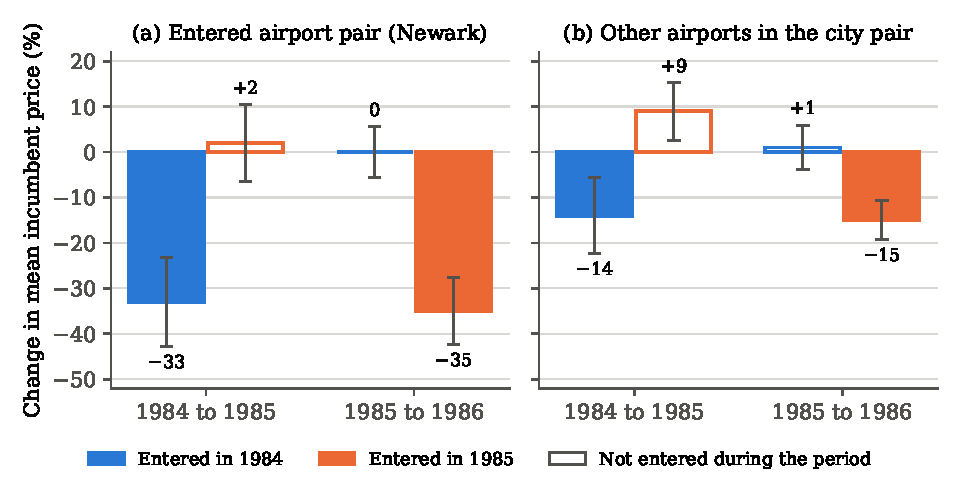
\includegraphics[width=\linewidth]{figures/ch09/wc_did.pdf}
\caption{Percentage change in the mean incumbent price by entry cohort and period. Filled bars are the
cohort entered during the period, and open bars the cohort not entered during it. Whiskers show plus
or minus one standard error of the cohort mean, computed as the reported cross-market standard
deviation divided by $\sqrt{n}$ ($n=7$ and $8$). Redrawn from \citet{WhinstonCollins1992}, Tables~3
and~4.}
\label{fig:09-wc-did}
\end{figure}

\casehead{Prices}
The pattern is similar in the two periods (p.~459). In markets entered during a
year, the mean incumbent price fell by about 35 percent. In markets not entered that year it barely
moved. The two contrasts are $-35$ points each, with $t$ statistics of 2.5 and 3.5. Their equality is
consistent with the three assumptions. So are the 2 percent rise in the 1985 cohort's prices before
its entry and the flat prices of the 1984 cohort in the year after its entry. None of these patterns
confirms the assumptions, because offsetting departures from them reproduce all four changes. Suppose the true
effect is $-25$ points and fades by 10 points in its second year. Suppose also that, without entry,
prices in the 1984 cohort would have fallen 10 points more than in the 1985 cohort in 1984--1985. Let
prices in the 1985 cohort rise 2 points in 1984--1985, as observed. Let all prices fall 10 points in 1985--1986 for reasons unrelated to entry. These values give exactly the
changes $-33$, $+2$, $0$ and $-35$ of Panel~A. Even after the cuts, People Express's average fare in the first
quarter after entry was 19 percent below the incumbents' mean fare.

Price dispersion fell, or rose less, in entered markets. The contrast is larger in 1984--1985 ($-55$
points, $t=2.6$) than in 1985--1986 ($-20$ points, $t=1.0$). The authors speculate that airlines grew
more skilled at \emph{yield management}, the dynamic allocation of seats across fare classes, over the
period. By 1985--1986 an incumbent could target its price
cuts where they mattered most, without lowering all fares.

\casehead{Quantities and revenue}
Incumbents sold more tickets after entry, if anything. The contrasts are $+72$ and $+74$ points, but
the variation across markets is large and neither is significant. Revenue fell much less than the price
cuts alone would imply (n.~34). In 1984--1985, revenue in entered markets rose 21 percent (s.d.\
22) against 33 percent (s.d.\ 28) in markets not entered. In 1985--1986 the figures are 3 percent
(s.d.\ 29) and 10 percent (s.d.\ 16). Revenue understates the incumbents' loss, because carrying more
passengers raises costs and, as we see next, incumbents also added capacity.

\casehead{Capacity}
The authors compared incumbents' nonstop seats on the entered route one year after the announcement
with seats at the announcement, using the \emph{Official Airline Guide}. Seats rose 25 percent on
average (s.d.\ 42). Domestic seats at Newark offered by carriers other than People Express rose 11
percent a year over 1984--1986. That benchmark includes the entered markets, so the comparison
understates the gap (n.~35). Nearly all of the increase came from flight frequency. Seats per
flight rose only 6 percent (s.d.\ 20), against 3 percent at Newark. The capacity increases were larger
for the 1984 cohort, 48 percent (s.d.\ 52), than for the 1985 cohort, 5 percent (s.d.\ 14)
(n.~36).

\casehead{Other airports in the city pair}
Panel~B shows the same pattern on a smaller scale (pp.~460--461). Prices fell 14 and 15 percent
in the treated cohorts, the ``15\%'' the paper quotes, while the control cohorts' prices rose 9 and 1
percent. The contrasts are $-23$ points ($t=2.1$) and $-16$ points ($t=2.3$). Quantity changes are
small and insignificant. Incumbent capacity on these routes rose 1 percent (s.d.\ 30) in the year
after entry, against a 1 percent decline at Kennedy and La Guardia. Seats per flight fell 4 percent
(s.d.\ 9), against a 2 percent decline at those airports, so frequency again rose. Price dispersion
again fell relative to controls, more in 1984 than in 1985. The smaller price response matches the
small $\mathit{OSM}$ value effect. Airports in a city are substitutes, but imperfect ones.

\casehead{Interpretation}
The quantity and capacity responses discriminate among models of competition (p.~460). Under
price taking, each incumbent sells where price equals its marginal cost. Entry lowers the market price
and moves each incumbent down its supply curve, so its output falls. Price cuts together with rising
sales and capacity are hard to square with any simple price-taking model. The rents revealed by the
value losses are therefore not the efficiency rents of a competitive market.

Static oligopoly models predict the same direction as price taking. In symmetric Cournot competition
each firm's output falls when the number of firms rises \eqref{eq:09-cournot-entry}, and by
\cref{rem:09-ks} the same holds for capacities. By \eqref{eq:09-br-slope}, the observed responses fit
static models only if quantities are strategic complements, which requires unusually convex demand.
They are consistent with a dynamic strategy. Industry observers
claimed that incumbents responded aggressively to induce exit, or at least to discourage further
expansion. The larger capacity increases in 1984 fit this interpretation. The responses also show that
the value losses did not reflect a temporary adjustment toward a smaller scale of operations.

The authors add a caution (pp.~458--459). Demand or cost conditions may have changed in the
entered markets, and such changes might even have caused entry. The size of the effects and the view
that the events reflected People Express's own strategy make it plausible that most of the change is
a response to entry.

\subsection{Conclusions, limitations, and contribution}\label{sec:09-wc-concl}

\casehead{What the paper concludes, and where}
\Cref{tab:09-wc-claims} lists each conclusion of the paper with the evidence and the test behind it.
The value results come from the $\mathit{SM}$ rows of \cref{tab:09-wc-t1,tab:09-wc-t2}. The contrast
between airports comes from the $\mathit{OSM}$ rows and the test of equal effects. The general effects
come from the fixed-effect sums. The incumbent responses come from \cref{tab:09-wc-t34} and the
schedule comparisons.

\begin{table}[htbp]
\centering
\caption{Conclusions of Whinston and Collins (1992) and the supporting evidence}
\label{tab:09-wc-claims}
\footnotesize
\begin{tabularx}{\linewidth}{@{}>{\raggedright\arraybackslash}p{0.27\linewidth}
  >{\raggedright\arraybackslash}X >{\raggedright\arraybackslash}p{0.25\linewidth}@{}}
\toprule
Conclusion & Evidence & Test\\
\midrule
Route-specific profits or sunk costs exist, so airline routes are not contestable &
$\lambda_{SM}<0$ in all windows (Table 1) and all specifications (Table 2, SM row). Loss of \$3.7 to
\$6.5 million per incumbent & $t$ tests of $\lambda_{SM}=0$: $-2.98$ to $-3.15$ (Table 1), $-2.18$
(Table 2, column 5)\\
\addlinespace
Local market structure matters, and profits are not equalized across routes &
Incumbency loss survives firm fixed effects. An incumbent loses \$6.2 million versus \$1.9 million
for a non-incumbent (Table 2, column 5) & $t$ test of $\lambda_{SM}$ with fixed effects, fixed-effect
sum\\
\addlinespace
Airports in the same city are differentiated &
$\lambda_{OSM}$ small, positive, insignificant (Table 2, columns 3 to 5) & Test of
$\lambda_{SM}=\lambda_{OSM}$, rejected at 2.5 percent\\
\addlinespace
Large industry-wide effects of unclear origin & Sum of fixed effects $-\$36.2$ million, over 80
percent of industry loss (Table 2, column 5) & Standard error of the sum, quasi-likelihood ratio test
of New York versus other fixed effects\\
\addlinespace
Incumbents cut prices sharply but raised capacity and sales &
Price contrasts of $-35$ points on the entered pair and $-23$ and $-16$ at other airports. Seats $+25$
percent (Tables 3 and 4, schedule data) & Two-sample $t$ tests with 13 degrees of freedom\\
\bottomrule
\end{tabularx}

\smallskip
\parbox{0.97\linewidth}{\footnotesize Notes: Table numbers refer to \citet{WhinstonCollins1992}, reproduced
here as \cref{tab:09-wc-t1,tab:09-wc-t2,tab:09-wc-t34}.}
\end{table}

\casehead{From descriptive results to economic inferences}
The chain of reasoning has three links. The first is statistical. Incumbents' abnormal dollar
changes on announcement days are negative and proportional to their seat-miles on the entered route.
The second is the efficient-markets link. Under (E1) to (E5) the abnormal change equals the change in
expected discounted profits caused by the news. The third is theoretical. By \cref{prop:09-valueloss},
a loss of expected profits from entry implies pre-entry rents or sunk costs, which contestability
excludes. Each richer specification in \cref{tab:09-wc-t2} rules out an alternative reading of the
first link. Slot rents at nearby airports, general industry effects and connecting markets cannot
account for the incumbency loss.

\casehead{Advantages over pricing regressions}
The event study needs no model of the network, and no controls for each route's demand and cost.
The variation comes from the timing of announcements and from incumbents' exposure, which People
Express's strategy determined. The method also measures the level of rents in dollars, as a lower
bound, where a pricing regression delivers a correlation between fares and structure.

\casehead{Limitations}
The design has several limitations, some noted by the authors and some raised by the logic of the
method.
\begin{itemize}
\item The sample is small. There are 24 events on 17 dates, and 22 involve Newark. The general effects
use 19 parameters, and the non-New York effects rest on two events.
\item Dating and anticipation bias the estimates toward zero. People Express's expansion was public
and ongoing, so markets probably expected some entry. Later work on Southwest finds that incumbents cut
fares once entry becomes likely, before the entrant starts flying \citep{GoolsbeeSyverson2008}. News
about entry can therefore arrive well before any announcement.
\item The general effects remain unexplained. Information about People Express's future scale,
competitive spillovers and aircraft values cannot be separated. If informational effects are
correlated with incumbency, part of the $\mathit{SM}$ effect could be informational. The separate New
York effects address this only partly.
\item Entry into a carrier's markets might signal that People Express intended to ``go after'' that
carrier. This informational effect would also load on incumbency. The authors see no way to control for
it without strong assumptions about its form, and they find little evidence of such a pattern (n.~25).
\item Seat-miles measure capacity. They do not count passengers. Connecting traffic is not controlled for, and the
loss per seat is assumed common across routes up to the robustness checks of footnote~32.
\item The bound $L\le V^0+K$ cannot separate pre-entry profits from sunk costs. The value change also
embeds the expected post-entry game, including the incumbents' own aggressive responses.
\item External validity is limited. People Express was a special entrant, with a new low-frill product
and low labor costs, in a transitional period after deregulation.
\item The price and capacity evidence uses 7 and 8 markets, with no formal control for changes in
demand. Only one year precedes the entry of both cohorts. The design therefore cannot separate
differential trends from effects that change after entry, and offsetting departures pass its one
testable restriction. If incumbents moved aircraft from control markets into entered markets, the control group is
affected by entry and the quantity contrasts are overstated.
\end{itemize}

\casehead{Contribution}
\citet{WhinstonCollins1992} gave a market-based test of contestability that does not depend on
controls for route demand and cost. Their incumbency loss confirms the conclusion of the pricing
studies that local structure matters, and it adds a dollar measure of rents. They gave market-based
evidence that airports serving the same city are differentiated, and they documented large
industry-wide effects of entry announcements. Their price and capacity evidence showed incumbents
responding to a low-fare entrant with deep price cuts and more capacity. The abnormal-dollar
formulation, with exposure measures that vary across firms, carries over to event studies of mergers
(\cref{ch:mergers}). \Cref{sec:09-synthesis} compares what this design identifies with the pricing
regressions of \cref{sec:09-borenstein} and the structural model of \cref{sec:09-bcs}.

\section{Hubs, costs, and markups: Berry, Carnall and Spiller (2006)}\label{sec:09-bcs}

\citet{BerryCarnallSpiller2006} bring the question of \cref{sec:09-borenstein} into the framework of
\cref{sec:09-pricing}. On ticket data of the same kind, they estimate a differentiated-products demand
system with two consumer types, a network model of marginal cost and a static Nash pricing equilibrium.
The model separates the two channels through which a hub can change the hub carrier's fares: higher markups
and lower costs. This section follows their analysis from the question to the conclusions, and
\cref{tab:09-bcs-map} at its end maps the study. As throughout the chapter, page, table, figure and footnote numbers refer to the 1996 working paper
\citep{BerryCarnallSpiller1996}.

\subsection{The question}\label{sec:09-bcs-question}

\Cref{sec:09-hubs} described the two views of hubs that coexisted by the mid-1980s. Critics held that hubs
raise entry barriers and fares for passengers who start their trips at a hub. Carriers and some economists
held that hubs reduce costs. The two effects are not mutually exclusive \citep{Berry1990}. A hub can raise
the markup over marginal cost for some travelers and lower marginal cost at the same time. On the demand
side, Berry, Carnall and
Spiller think of a hub as shifting out the demand for the hubbing carrier's flights out of its hub city.
Those flights may appeal especially to price-inelastic consumers, so the shift can also make demand less
elastic (p.~1). On the cost side, densely traveled spokes may have lower marginal costs. Economies of spoke
density then create economies of scope across itineraries that share a spoke (p.~2).

A fare regression cannot separate the two effects. Write the fare of product $j$ as $p_j=mc_j+m_j$, with
$m_j$ the markup. If hub presence raises $m_j$ and lowers $mc_j$, the change in the fare is
\begin{equation*}
\Delta p_j=\Delta m_j+\Delta mc_j,\qquad \Delta m_j>0,\quad \Delta mc_j<0 .
\end{equation*}
A regression of fares on hub presence estimates the sum. Without a model of markups or of costs it cannot
recover the two terms. As the authors note, \citet{Borenstein1989} has no model of costs or demand. In
their words, he ``attempts to control for market-level unobservables by, for example, introducing
city-pair level fixed effects'' (p.~5). His relative-price equation \eqref{eq:09-bor-rel} has the same
effect, since it differences out everything common to the carriers on an airport-pair route.
\citet{BruecknerSpiller1994} take the
opposite route. They estimate density economies from itineraries that pass through hubs without
originating there, to avoid hub markups (p.~4). That choice discards the markets where hub effects should
be largest. In the authors' words, reduced form regressions ``do not allow us to make statements about how
prices relate to costs, or what are the determinants of markups over cost'' (p.~6).

The strategy of the paper is to treat hub presence as one characteristic in a differentiated-products
model of demand. Combined with a cost model and an equilibrium assumption, the demand model yields a
markup for every product. Marginal cost is then ``observed'' as price minus the model's markup (p.~5), and
its relation to spoke density reveals economies of density. The model is the finite-mixture nested logit
of \cref{sec:09-pricing-types} with $R=2$ types, combined with the network costs of
\cref{sec:09-pricing-network}. The authors summarize their findings in five claims (abstract and
pp.~2--3), which we examine against their tables below.
\begin{enumerate}[label=(\roman*)]
  \item Travelers come in two distinct types. One has the attributes of a tourist: high price sensitivity
  and low willingness to pay for frequent-flyer features, frequency and nonstop service. The other has
  those of a business traveler.
  \item Hubs give the hub carrier two advantages: lower costs and higher markups on hub-originating
  passengers.
  \item The hub carrier's ability to raise prices is focused on business travelers. They shift toward the
  hub carrier even though they pay a premium of about 20\% over non-hub carriers.
  \item The hub carrier does not provide a ``monopoly umbrella'' to its rivals. Non-hub carriers lose
  business travelers and market share at the same time, which the authors call a ``competitive scissor.''
  \item There are economies of density on longer routes and none on routes shorter than about 500 miles,
  which the authors call the ``Southwest effect.''
\end{enumerate}

\subsection{Data}\label{sec:09-bcs-data}

The data come from the DOT ticket sample (DB1A) and the Service Segment Databank (DB27R) described in
\cref{sec:09-data}, for the fourth quarter of 1985 (p.~19). The quarter follows \citet{BruecknerDyerSpiller1992}
and \citet{BruecknerSpiller1994}. Those studies used only four-segment round trips that did not originate at
hub cities, to avoid demand-side hub effects. Berry, Carnall and Spiller model hub markups explicitly, so
they keep hub origins and itineraries with any number of segments up to two per direction. The ticket
conventions are those of \cref{sec:09-data}: round trips only, without itineraries chosen by a single
sampled passenger and without extreme fares. Southwest is absent, because it reported all its sales as one-way
tickets and so did not fit the product definition (p.~14, n.~11). The quarter precedes the merger wave of
1986--1987 and Borenstein's sample from 1987.

The unit of observation is a \emph{product} $j$, a unique combination of carrier, itinerary and fare in a
directional city-pair market $t$ (\cref{sec:09-data}). The sample has 122,871 products in 14,122 markets.
The products use 4,963 distinct carrier legs, flown by 32 carriers out of 262 origins, and represent
1,107,894 sampled passengers (p.~19). About 30\% of the markets have a single product and another 30\% have
no more than five. About 1\% have more than one hundred products, with a maximum of 874 in the New York to
Miami market. The quantity $q_{jt}$ is the number of sampled passengers (NPASS) and the price $p_{jt}$ is
the round-trip fare (FARE). Market size is built from $\mathit{MPOP}_t$, the geometric mean of the two
endpoint populations, $\sqrt{\text{origin population}\times\text{destination population}}$ (Appendix). A
\emph{leg} $\ell$ is a nonstop segment flown by one carrier. Its density $Q_\ell$ comes from DB27R and
adds the two directions, because the trips are round trips (Appendix, n.~4).

A structural model has more than one dependent variable. Each product contributes two endogenous outcomes,
its market share and its fare, and leg densities are endogenous as well. The inversion of demand turns the
share into the demand error $\xi_{jt}$. The pricing condition turns the fare into the cost error
$\omega_{jt}$. The regressors are the product and market characteristics in \cref{tab:09-bcs-vars} and the
leg cost terms. The instruments are discussed in \cref{sec:09-bcs-estimation}.

\begin{table}[htbp]
\centering
\begin{threeparttable}
\caption{Variables in the model of Berry, Carnall and Spiller}
\label{tab:09-bcs-vars}
\footnotesize
\begin{tabularx}{\textwidth}{@{}>{\raggedright\arraybackslash}p{2.2cm}>{\raggedright\arraybackslash}X
  >{\raggedright\arraybackslash}p{2.6cm}@{}}
\toprule
Variable & Definition (units) & Role \\
\midrule
\multicolumn{3}{@{}l}{\textit{Demand side (product $j$ of carrier $f$ in market $t$)}}\\
FARE & Round-trip fare (\$100) & Type-specific ($\alpha_r$) \\
DIRECT & 1 if the itinerary has one segment, 0 if it has two & Type-specific \\
HUBSIZE & If the origin is a hub of carrier $f$: the sum of the population potentials of all city pairs
  that $f$ connects through that hub. Zero otherwise & Type-specific \\
TEMPDIFF & Difference between the mean January temperatures of origin and destination (10\textdegree F) &
  Type-specific, market level \\
TRIPS-D & Minimum over the itinerary's legs of $f$'s departures on the leg (1,000 per quarter) &
  Type-specific \\
CONSTANT & 1 & Common \\
CONGEST-D & Number of endpoints (0, 1 or 2) that are slot controlled & Common, market level \\
MDIST, MDIST$^2$ & Great-circle distance between the endpoints (1,000 miles), and its square & Common, market
  level \\
\addlinespace
\multicolumn{3}{@{}l}{\textit{Cost side (summed over the legs $\ell\in\mathcal{L}(j)$ of the itinerary)}}\\
NSEGS & Number of legs (1 or 2) & Leg constant \\
CONGEST-S & Takeoffs and landings at the four slot-controlled airports (0 to 4) & Leg cost shifter \\
CONGEST-C & Takeoffs and landings at the 24 airports under FAA flow control (0 to 4) & Leg cost shifter \\
DIST, DENS & Leg distance $d_\ell$ (1,000 miles) and leg density $Q_\ell$ (100,000 passengers per quarter,
  both directions), with powers and interactions & Cubic polynomial \\
TRIPS-C & Leg departures $F_\ell$ (1,000 per quarter) & Column IV only \\
\bottomrule
\end{tabularx}
\begin{tablenotes}\footnotesize
\item Notes: The population potential of a city pair is the geometric mean of the two populations. The
slot-controlled airports are Chicago O'Hare, New York Kennedy and La Guardia, and Washington National
(p.~20, n.~13). The flow-control list includes Orange County and Long Beach (p.~21, n.~14). The text calls
the slot-control count CONGEST-C and the flow-control count DOT-CONGEST, while Tables 3 and 5 label the
cost-side congestion variables CONGEST-S and CONGEST-C. We match the labels by their sample means in
Table~3 (0.315 and 1.766), which equal the appendix means of the slot-control count (0.3149) and of the
flow-control count (1.7656). Source: \citet{BerryCarnallSpiller1996}, pp.~20--21 and Appendix.
\end{tablenotes}
\end{threeparttable}
\end{table}

\Cref{tab:09-bcs-desc} reproduces the descriptive statistics. The mean round-trip fare is \$276 with a
standard deviation of \$149. The number of sampled passengers per product has mean 9.0, standard deviation
31.3 and maximum 2,798, so most products are bought by very few sampled passengers. This fact matters for
the sampling error discussed in \cref{sec:09-bcs-estimation}. Slightly fewer than half of the products
(46.6\%) have a single segment. HUBSIZE is zero for most products, with mean 0.017 and standard deviation
0.045. Second-leg distances and densities are set to zero for one-segment products (p.~21), which explains
their low means. In the appendix statistics the means of DIRECT and NSEGS are 0.4666602 and 1.5333398,
which sum to exactly two, and their standard deviations are identical. In this sample DIRECT therefore
equals $2-\mathit{NSEGS}$, so ``direct'' means a single segment.

\begin{table}[htbp]
\centering
\begin{threeparttable}
\caption{Descriptive statistics, 122,871 origin-destination-fare-carrier products}
\label{tab:09-bcs-desc}
\small
\begin{tabular}{@{}lrrrr@{}}
\toprule
Variable & Mean & Std.\ dev. & Min & Max \\
\midrule
FARE (\$100) & 2.764 & 1.488 & 0.110 & 18.33 \\
NPASS (passengers) & 9.017 & 31.299 & 1.000 & 2798.0 \\
DIRECT (fraction) & 0.466 & 0.498 & 0.000 & 1.000 \\
HUBSIZE & 0.017 & 0.045 & 0.000 & 0.210 \\
TEMPDIFF (10\textdegree F) & 0.286 & 2.077 & $-6.520$ & 6.520 \\
TRIPS-D (minimum, 1,000 per quarter) & 0.293 & 0.179 & 0.001 & 1.595 \\
CONGEST-D (number of airports) & 0.202 & 0.413 & 0.000 & 2.000 \\
MDIST (1,000 miles) & 1.009 & 0.608 & 0.030 & 2.776 \\
\addlinespace
DIST, first outbound leg (1,000 miles) & 0.710 & 0.503 & 0.021 & 2.704 \\
DIST, second outbound leg (1,000 miles) & 0.351 & 0.479 & 0.000 & 2.611 \\
DENS, first outbound leg (100,000 per quarter) & 0.593 & 0.475 & 0.00003 & 4.553 \\
DENS, second outbound leg (100,000 per quarter) & 0.361 & 0.493 & 0.000 & 4.553 \\
TRIPS-C, first leg (1,000 departures per quarter) & 0.349 & 0.214 & 0.001 & 1.595 \\
TRIPS-C, second leg (1,000 departures per quarter) & 0.212 & 0.249 & 0.000 & 1.594 \\
\bottomrule
\end{tabular}
\begin{tablenotes}\footnotesize
\item Notes: Statistics across products. Second-leg values are zero for one-segment products.
Source: \citet{BerryCarnallSpiller1996}, Table~1.
\end{tablenotes}
\end{threeparttable}
\end{table}

The raw correlations among the endogenous variables point the wrong way for a naive test of density
economies (Table~2). Price is positively correlated with the densities of the first and second outbound legs
(0.084 and 0.122). Price and the number of passengers are negatively correlated ($-0.063$). The number of
passengers is correlated with the first-leg density at 0.068 and with the second-leg density at $-0.120$,
and the two densities are correlated at 0.164. The authors read the positive price-density correlations as
evidence that one must control for markups and distance before economies of density can appear (p.~21). One
reason is that dense legs connect large cities and hubs, where demand and markups may be high. In a
subsample of small four-segment markets, the sampling frame of Brueckner and Spiller, the raw correlation
between price and density is negative (p.~21, n.~15).

\subsection{Demand}\label{sec:09-bcs-demand}

\casehead{Market size}
The model needs an outside good, and hence a number of potential trips in each market. Berry, Carnall and
Spiller assume that this number is proportional to the geometric mean of the endpoint populations,
$M_t=\kappa\,\mathit{MPOP}_t$, with $\kappa$ a parameter to be estimated (p.~9). Each potential trip is
treated as a separate consumer, with no correlation of tastes across trips by the same person. The
observed shares are therefore functions of $\kappa$:
\begin{equation}\label{eq:09-bcs-sobs}
s^{obs}_{jt}(\kappa)=\frac{q_{jt}}{\kappa\,\mathit{MPOP}_t},\qquad
s^{obs}_{0t}(\kappa)=1-\sum_{j\in\mathcal{J}_t}s^{obs}_{jt}(\kappa).
\end{equation}
Because $q_{jt}$ counts passengers in a 10\% sample, $\kappa$ also absorbs the sampling rate.

\casehead{Unobserved product characteristics}
The term $\xi_{jt}$ captures ticket restrictions, such as advance-purchase and Saturday-stay requirements,
together with unmeasured quality such as food and service (p.~9). Firms and consumers observe it. Tickets
with different restrictions have systematically different prices, so $\xi_{jt}$ is correlated with price
by construction and price is endogenous. The authors assume instead that $\xi_{jt}$ is mean independent of
the other observed characteristics, such as distance and DIRECT. They defend this assumption with an
extreme case. Suppose every carrier offers the same menu of restrictions on every itinerary, for example
an unrestricted fare, an advance-purchase fare with a Saturday stay, and an advance-purchase fare without
one. Then the restrictiveness of a ticket is unrelated to $x_{jt}$. The authors concede that ``it is not
hard to think of stories which would violate'' the assumption (p.~9). A hub carrier that sells relatively
more unrestricted fares out of its hub would be one such story, since $\xi_{jt}$ would then rise with
HUBSIZE.

\casehead{Utility}
A potential traveler $i$ in market $t$ is of type $r\in\{1,2\}$, with $\Pr(r=1)=\psi$ and $\Pr(r=2)=1-\psi$.
In the notation of \cref{ass:09-fm}, a type-$r$ traveler has utility
\begin{equation}\label{eq:09-bcs-utility}
u_{ijt}=\delta^r_{jt}+\zeta_{igt}+(1-\sigma)\epsilon_{ijt}\quad(j\in\mathcal{J}_t),\qquad
u_{i0t}=\epsilon_{i0t},
\end{equation}
with type-specific mean utility
\begin{equation}\label{eq:09-bcs-delta-r}
\begin{aligned}
\delta^r_{jt}={}&\beta_0+\beta^{M}\mathit{MDIST}_t+\beta^{MM}\mathit{MDIST}_t^2+\beta^{C}\mathit{CONGEST\text{-}D}_t\\
&+\beta^{D}_r\mathit{DIRECT}_j+\beta^{h}_r\mathit{HUBSIZE}_{jt}+\beta^{T}_r\mathit{TEMPDIFF}_t
+\beta^{F}_r\mathit{TRIPS\text{-}D}_j-\alpha_rp_{jt}+\xi_{jt}.
\end{aligned}
\end{equation}
All inside goods form one nest and the outside good forms the other. Berry, Carnall and Spiller write the
idiosyncratic term as $\nu_i(\lambda)+\lambda\epsilon_{ij}$ (p.~11). In our notation $\lambda=1-\sigma$,
their $\nu_i(\lambda)$ is $\zeta_{igt}$, their type-1 probability $\gamma$ is $\psi$, and their market-size
factor $\mu$ is $\kappa$. As $\sigma\to0$ the choices within a market become uncorrelated and the model
reduces to a mixture of two logits. As $\sigma\to1$ the correlation of choices within the market goes to
one (p.~12).

\casehead{Shares}
Specializing \eqref{eq:09-fm-shares} to two types, the shares of a type-1 traveler are (p.~12)
\begin{equation}\label{eq:09-bcs-shares}
s^1_{j|g,t}=\frac{e^{\frac{\delta^1_{jt}}{1-\sigma}}}{D_{1t}},\qquad
D_{1t}=\sum_{k\in\mathcal{J}_t}e^{\frac{\delta^1_{kt}}{1-\sigma}},\qquad
\bar s_{1t}=\frac{D_{1t}^{1-\sigma}}{1+D_{1t}^{1-\sigma}},\qquad
s^1_{jt}=s^1_{j|g,t}\,\bar s_{1t},
\end{equation}
and the type-2 shares have the same form with $\delta^2_{jt}$. The predicted share of product $j$ is the
type-weighted average
\begin{equation}\label{eq:09-bcs-sj}
s_{jt}=\psi\,s^1_{jt}(p_t,x_t,\xi_t)+(1-\psi)\,s^2_{jt}(p_t,x_t,\xi_t).
\end{equation}

\casehead{Why two types}
\Cref{sec:09-pricing-types} gave the reasons why business travelers are less sensitive to price than
leisure travelers and why tastes are correlated across characteristics (p.~10, n.~9). A two-point
distribution is the simplest
bimodal distribution with correlated tastes (p.~10). The fat upper tail of fares per mile discussed in
\cref{sec:09-data} supports it. A mixture of two normal distributions fits that distribution far better than a
single normal. The authors compare the two components of that mixture with the estimated
model (p.~11, n.~10). The components are $N(0.2375, 0.0781)$ and $N(0.5946, 0.2752)$, so the second is
also far more dispersed. The model's mean fare per mile for type 1, 0.237, equals the mean of the first
component (0.2375). For type 2 the model gives 0.414, against 0.589 from the mixture.\footnote{The fitted
formula in footnote~10 gives the second component a mean of 0.5946, while the comparison in the same
footnote quotes 0.589. Likewise, the weight on the first component is 0.5987 in the formula and 0.598 in
the comparison. We report all four numbers as printed.} Type 1 accounts for 73\% of tickets in the model,
against a weight of 0.598 in the mixture. Five coefficients vary by type: those on FARE, DIRECT, HUBSIZE,
TEMPDIFF and TRIPS-D. By \cref{rem:09-discrete-rc}, two types need 11 parameters for these five
coefficients, against 10 for independent normal random coefficients, and they deliver closed-form shares.
The authors mention extensions they do not pursue (p.~11). Tastes could be drawn from two normal
distributions instead of two points, there could be more than two types, and nests could group airports
within a city or carriers within a market.

\casehead{The role of each characteristic}
The constant, MDIST, MDIST$^2$, CONGEST-D and TEMPDIFF are the same for every product in a market. They
shift the demand for air travel relative to the outside good (p.~20). They also cancel from each type's
within-nest shares $s^r_{j|g,t}$ in \eqref{eq:09-bcs-shares}. At given prices they therefore leave the
choice among flights of a traveler of either type unchanged. The paper concludes that TEMPDIFF ``has no
power to explain the choice between products'' (p.~20). This holds within a type. Aggregate shares can
still move, because these variables change the mix of types among the travelers who fly. By
\eqref{eq:09-bcs-sj}, the share of product $j$ among the inside goods is
\begin{equation*}
\frac{s_{jt}}{\sum_{k\in\mathcal{J}_t}s_{kt}}=\sum_{r=1}^{2}w_{rt}\,s^r_{j|g,t},\qquad
w_{1t}=\frac{\psi\,\bar s_{1t}}{\psi\,\bar s_{1t}+(1-\psi)\,\bar s_{2t}},\qquad w_{2t}=1-w_{1t},
\end{equation*}
where $w_{rt}$ is the share of type $r$ among the travelers who fly. A change in a market-level variable
leaves each $s^r_{j|g,t}$ fixed and moves the weights. If it raises every type-$r$ mean utility by $c_r$,
then $\frac{\partial\ln\bar s_{rt}}{\partial c_r}=1-\bar s_{rt}$. The weights therefore change when the
coefficient differs across types, as for TEMPDIFF. They also change under a common coefficient whenever
the two types' inside shares differ. The aggregate choice among flights then shifts toward the flights
that the type gaining weight prefers. DIRECT, HUBSIZE and TRIPS-D vary across carriers and itineraries within a market,
so they also govern substitution among flights within each type. HUBSIZE weights each city pair the carrier connects through its hub by
the pair's population potential. The authors prefer it to a hub dummy or to the number of points served,
neither of which accounts for the relative importance of the city pairs (p.~20). TEMPDIFF measures appeal to
tourists. Because its coefficient varies by type, it shifts the type mix and can help separate the types
(p.~20).

The model lets hub presence affect markups through the composition of buyers. By \eqref{eq:09-composition},
product $j$'s buyers are of type 2 with probability $\Pr(2\mid j)=\frac{(1-\psi)s^2_{jt}}{s_{jt}}$. By
\cref{prop:09-composition-markup} and \cref{rem:09-fm-extensions}, a single-product markup is close to
$\frac{1-\sigma}{\bar\alpha_j}$ when within-nest shares are small, where
$\bar\alpha_j=\Pr(1\mid j)\alpha_1+\Pr(2\mid j)\alpha_2$. If $\beta^h_2>\beta^h_1$ and $\alpha_2<\alpha_1$,
a larger HUBSIZE tilts the buyers of the hub carrier's products toward type 2, lowers $\bar\alpha_j$ and
raises the markup. Because $\Pr(2\mid j)$ is a logistic function of $\ln s^2_{jt}-\ln s^1_{jt}$, its shift
is proportional to $\Pr(2\mid j)\big(1-\Pr(2\mid j)\big)$ and is largest near an even mix. The markup
$\frac{1-\sigma}{\bar\alpha_j}$ is convex in $\Pr(2\mid j)$, however. With the column III price coefficients,
the markup response is largest for products whose buyers are already about 90\% type 2.

\subsection{Costs and pricing}\label{sec:09-bcs-supply}

\casehead{Leg costs and product marginal cost}
The cost side follows \citet{BruecknerSpiller1994}, as in \cref{sec:09-pricing-network}. Leg $\ell$ of carrier
$f$ has total cost $C_\ell(Q_\ell,w_\ell)$ and marginal cost $c_\ell(Q_\ell,w_\ell)$, where $w_\ell$
includes the leg's distance and the characteristics of its endpoint airports (p.~13). The carrier's cost is
\eqref{eq:09-firm-cost}, and the marginal cost of product $j$ is \eqref{eq:09-itin-mc}, the sum of its legs'
marginal costs plus a product-specific term $\omega_{jt}$. The authors give the product-specific cost the
form $\omega_{jt}q_{jt}$ only so that marginal cost has an additive error (p.~13). Fixed costs may also fall
with hubbing, but the model uses only marginal costs and cannot capture that effect.

\casehead{Prior beliefs about distance, density and frequency}
The authors expect a complicated relation among distance, density and flight frequency (pp.~13--14). On short
routes air travel competes with cars and, in a few places, trains. Carriers may then spend density savings
on more frequent flights, which let travelers choose departure times precisely. The East and West Coast
shuttles and Southwest are examples. On short routes large aircraft may also not pay, because takeoffs and
landings are a large share of cost. That cost does not vary with distance and is not offset by savings in
the air. The data have no model of frequency but do report quarterly trips on each leg. Frequency enters
some specifications as an exogenous cost shifter. These considerations call for a flexible functional form.

\casehead{The leg marginal cost function}
Segment marginal cost is a cubic polynomial in leg distance $d_\ell$ (1,000 miles) and leg density $Q_\ell$
(100,000 passengers per quarter), with congestion shifters. Write $\chi_{mn}$ for the coefficient on
$d_\ell^mQ_\ell^n$, and $n^S_\ell$ and $n^C_\ell$ for the leg's takeoffs and landings at slot-controlled and
at flow-control airports. In columns I to III of Table~5, leg marginal cost in \$100 is
\begin{equation}\label{eq:09-bcs-mc}
\begin{aligned}
c_\ell={}&\chi_{00}+\chi_{10}d_\ell+\chi_{20}d_\ell^2+\chi_{30}d_\ell^3
+\chi_{01}Q_\ell+\chi_{02}Q_\ell^2+\chi_{03}Q_\ell^3\\
&+\chi_{11}d_\ell Q_\ell+\chi_{21}d_\ell^2Q_\ell+\chi_{12}d_\ell Q_\ell^2
+\chi_S n^S_\ell+\chi_C n^C_\ell .
\end{aligned}
\end{equation}
Column IV adds nine terms in leg departures $F_\ell$ (1,000 per quarter):
\begin{equation}\label{eq:09-bcs-mc-trips}
\sum_{k=1}^{9}\chi^F_k\,h_k(F_\ell,d_\ell,Q_\ell),\qquad
(h_1,\dots,h_9)=(F,\,F^2,\,F^3,\,Fd,\,Fd^2,\,F^2d,\,FQ,\,F^2Q,\,FQ^2),
\end{equation}
with the leg subscripts dropped inside the list. Summing \eqref{eq:09-bcs-mc} over the legs of product $j$,
\begin{equation}\label{eq:09-bcs-mc-product}
mc_{jt}=\chi_{00}\,\mathit{NSEGS}_j+\chi_{10}\sum_{\ell\in\mathcal{L}(j)}d_\ell
+\dots+\chi_{12}\sum_{\ell\in\mathcal{L}(j)}d_\ell Q_\ell^2
+\chi_S\,\mathit{CONGEST\text{-}S}_j+\chi_C\,\mathit{CONGEST\text{-}C}_j+\omega_{jt}.
\end{equation}
The leg constant summed over legs becomes the coefficient on the number of segments. The mean of
$\omega_{jt}$, written $\bar\omega$, enters as a separate constant in product marginal cost (p.~21). Table~5
does not report it. Because NSEGS takes the values 1 and 2, $\bar\omega$ and $\chi_{00}$ are separately
identified.

Economies of density on leg $\ell$ mean that the leg's marginal cost falls as its density rises. From
\eqref{eq:09-bcs-mc},
\begin{equation}\label{eq:09-bcs-dcdq}
\frac{\partial c_\ell}{\partial Q_\ell}=\chi_{01}+2\chi_{02}Q_\ell+3\chi_{03}Q_\ell^2
+\chi_{11}d_\ell+\chi_{21}d_\ell^2+2\chi_{12}d_\ell Q_\ell ,
\end{equation}
and the leg has economies of density at $(d_\ell,Q_\ell)$ when this derivative is negative. In
\cref{ex:09-hubcost} the leg cost $aQ^\gamma$ has economies of density everywhere when $\gamma<1$. The
polynomial lets the sign vary with distance and density.

\casehead{What the cost model leaves out}
Prices, shares and densities are endogenous. Flight frequency is treated as exogenous. The data aggregate
traffic to the carrier, route and fare over a quarter, so they cannot show which flights are full or how
uncertainty about demand resolves before departure. The model therefore has no capacity constraints and no
demand uncertainty. The authors warn that ``some of what we label as a markup in fact represents a shadow
price of capacity'' (p.~14). Marginal cost may also vary with factors such as time-of-day capacity, which
the data do not record (p.~5).

\casehead{Pricing}
Following \citet{Berry1990}, prices form a static Nash equilibrium in which each carrier sets the prices of
all its products in all markets (pp.~6 and 14). The authors recognize that this is a simplification. Yield
management allocates seats across fare classes dynamically, and tacit collusion would add another layer,
but both are left for future work (p.~15). In the notation of \cref{sec:09-pricing-network}, carrier $f$'s
profit is (p.~15)
\begin{equation}\label{eq:09-bcs-profit}
\pi_f=\sum_t\ \sum_{j\in\mathcal{J}_f(t)}p_{jt}\,q_{jt}(p)-\sum_{\ell\in\mathcal{L}_f}C_\ell(Q_\ell,w_\ell)
-\sum_t\ \sum_{j\in\mathcal{J}_f(t)}\omega_{jt}\,q_{jt}(p)-FC_f .
\end{equation}
Differentiating with respect to $p_{jt}$ and exchanging the sums over legs and products, as in the
derivation of \eqref{eq:09-network-foc}, gives
\begin{equation}\label{eq:09-bcs-foc}
q_{jt}+\sum_{k\in\mathcal{J}_f(t)}\frac{\partial q_{kt}}{\partial p_{jt}}
\Big[p_{kt}-\omega_{kt}-\sum_{\ell\in\mathcal{L}(k)}c_\ell(Q_\ell,w_\ell)\Big]
=q_{jt}+\sum_{k\in\mathcal{J}_f(t)}\frac{\partial q_{kt}}{\partial p_{jt}}\,(p_{kt}-mc_{kt})=0 .
\end{equation}
Dividing by $M_t=\kappa\,\mathit{MPOP}_t$ turns quantities into shares. Stacking the conditions of market $t$
gives \eqref{eq:09-fm-markup}:
\begin{equation}\label{eq:09-bcs-markup}
p_t-mc_t=-\big[(\Omega_t\odot\Delta_t)^\top\big]^{-1}s_t,\qquad
\Delta_t=-\psi\,\alpha_1\frac{\partial s^1_t}{\partial\delta^1_t}-(1-\psi)\,\alpha_2\frac{\partial s^2_t}{\partial\delta^2_t},
\end{equation}
where the $(j,k)$ element of $\frac{\partial s^r_t}{\partial\delta^r_t}$ is given by
\eqref{eq:09-fm-derivs}.\footnote{The paper writes $p=\Delta^{-1}s+mc$ with $\Delta$ the matrix of
derivatives $\frac{\partial s_k}{\partial p_j}$ for products of the same firm (p.~15). That equation holds
when $\Delta$ contains the negatives of these derivatives. The paper's second expression,
$\Delta=\gamma\alpha_1\Delta_1+(1-\gamma)\alpha_2\Delta_2$ with $\Delta_r$ the derivatives with respect to
mean utility (p.~16), has the right sign. It equals $-(\Omega_t\odot\Delta_t)^\top$ in our notation. See
the footnote to \eqref{eq:09-fm-markup}.} Here $\Delta_t$ has $(j,k)$ element
$\frac{\partial s_{jt}}{\partial p_{kt}}$, as in \cref{ch:diffprod}.

Three features of \eqref{eq:09-bcs-markup} drive the empirical work. First, the markup depends only on the
demand parameters and on prices and shares (p.~16). It involves no cost parameter. Second, markups are not
profits. Airlines may be unprofitable even with large markups, because fixed costs may be large and marginal
cost may fall over a wide range of output (p.~16, \cref{rem:09-markups-profits}). Third, the network enters
the pricing condition only through the level of each $mc_{kt}$, evaluated at equilibrium densities.

\subsection{Estimation and identification}\label{sec:09-bcs-estimation}

\casehead{The estimator}
The parameters split into demand and cost parameters:
\begin{equation*}
\theta_d=(\sigma,\kappa,\psi,\alpha_1,\alpha_2,\beta_1,\beta_2),\qquad
\theta_c=(\bar\omega,\chi),\qquad \theta=(\theta_d,\theta_c).
\end{equation*}
Here $\beta_r$ collects type $r$'s taste coefficients, including the common
ones. The estimator follows \citet{Berry1994} and \citet{BerryLevinsohnPakes1995} (pp.~16--17). For a trial
value of $\theta$ it computes the two structural errors in five steps.
\begin{enumerate}[label=\arabic*.]
  \item Compute observed shares $s^{obs}_t(\kappa)$ from \eqref{eq:09-bcs-sobs}.
  \item Solve $s_t(\xi_t;\theta_d)=s^{obs}_t(\kappa)$ for $\xi_t(\theta_d)$ in each market, with the
  contraction \eqref{eq:09-fm-contraction}. \citet{Berry1994} guarantees a unique solution. The shares
  \eqref{eq:09-bcs-shares} and \eqref{eq:09-bcs-sj} are analytic, so no simulation is needed. With
  122,871 products the authors call this ``fortunate'' (p.~17).
  \item Evaluate $\Delta_t$ at $(p_t,\xi_t(\theta_d))$ and compute the markups
  $b_t(\theta_d)=-\big[(\Omega_t\odot\Delta_t)^\top\big]^{-1}s_t$ from \eqref{eq:09-bcs-markup}.
  \item Compute the cost error from \eqref{eq:09-bcs-mc-product}, with the observed densities as data:
  \begin{equation}\label{eq:09-bcs-omega}
  \tilde\omega_{jt}(\theta)=p_{jt}-b_{jt}(\theta_d)-\bar\omega-\sum_{\ell\in\mathcal{L}(j)}c_\ell(d_\ell,Q_\ell,n^S_\ell,n^C_\ell;\chi).
  \end{equation}
  \item Form the moments below and evaluate the objective.
\end{enumerate}
The identifying assumption is that both errors are mean independent of a vector of instruments $z_{jt}$:
\begin{equation}\label{eq:09-bcs-moments}
\E\left[\xi_{jt}(\theta_{d0})\given z_{jt}\right]=0,\qquad \E\left[\tilde\omega_{jt}(\theta_0)\given z_{jt}\right]=0 .
\end{equation}
With $N=122{,}871$ products and instrument matrices $Z^d_{jt}$ and $Z^c_{jt}$ built from $z_{jt}$, the
sample moments and the GMM estimator are
\begin{equation}\label{eq:09-bcs-gmm}
g_N(\theta)=\frac{1}{N}\sum_t\sum_{j\in\mathcal{J}_t}
\begin{pmatrix}Z^{d\top}_{jt}\,\xi_{jt}(\theta_d)\\ Z^{c\top}_{jt}\,\tilde\omega_{jt}(\theta)\end{pmatrix},
\qquad
\hat\theta=\argmin_\theta\ g_N(\theta)^\top W g_N(\theta),
\end{equation}
as in \cref{ch:blp}. Given $\theta_d$, the cost error is linear in $(\bar\omega,\chi)$. These parameters can
therefore be concentrated out by linear instrumental variables, like the linear parameters in
\cref{ch:blp}. The paper does not say how the search was organized.

\casehead{Instruments}
Price, shares and densities are endogenous. All other product and market characteristics are treated as
exogenous shifters of cost or demand, including the network structure of each carrier (pp.~17--18). The
instruments for leg densities include population and network characteristics at the endpoint cities. The
instruments for prices and markups add characteristics of the other products in the market (p.~18). The
authors chose the instrument vector by experimenting with simple versions of the model on a 10\% sample of
the data and then held it fixed for the full estimation (p.~18). The full list is not reported.

Each group of instruments rests on an economic argument. A product's own characteristics shift its demand
and, through the share, its markup. Rival products' characteristics shift the markup through the intensity
of competition, as in \citet{BerryLevinsohnPakes1995}. Population and network characteristics at the
endpoints shift a leg's density through traffic to and from other markets. Conditional on the included
characteristics, they are excluded from the product's own demand and cost errors. That exclusion requires
the network to be exogenous. If carriers built hubs where unobserved demand is high, network instruments
would be correlated with $\xi$. The paper does not model entry or network choice and refers to
\citet{Berry1990} and \citet{ReissSpiller1989} for that problem (p.~16, n.~12).

\casehead{Standard errors}
The errors are assumed independent across markets (p.~17). Within a market, demand and cost errors have a
factor structure, with market-specific components that are correlated across the demand and cost
equations. One parametrization consistent with this description is
\begin{equation}\label{eq:09-bcs-factor}
\xi_{jt}=a_t+e_{jt},\qquad \tilde\omega_{jt}=b_t+u_{jt},\qquad \Cov(a_t,b_t)\ne0,
\end{equation}
with $e_{jt}$ and $u_{jt}$ idiosyncratic. The structure enters the variance of the moments,
$V=\Var\big(\sum_{j\in\mathcal{J}_t}g_{jt}\big)$ summed over independent markets, where $g_{jt}$ is the
summand of \eqref{eq:09-bcs-gmm}. The asymptotic variance of $\hat\theta$ is then the usual sandwich
$(G^\top WG)^{-1}G^\top WVWG(G^\top WG)^{-1}$, with $G$ the derivative of the moments
(\cref{sec:A-gmm}). Treating each market as a cluster would be the nonparametric alternative.

\casehead{Sampling error in shares}
The inversion assumes that the econometrician observes expected shares \citep{Berry1994}. In
\citet{BerryLevinsohnPakes1995} shares were fractions of roughly 100 million households, so sampling error
was negligible. Here more than one million sampled passengers are spread over more than 120,000 products,
so the average product has fewer than 10 sampled passengers (p.~17). A rough calculation shows the
magnitude. If a product's sampled count $\hat n_j$ has mean $n_j$ and approximately Poisson variation, the
delta method gives $\Var(\ln\hat n_j)\approx\frac{1}{n_j}$. The standard deviation of the log share is then
about 0.33 at $n_j=9$ and 0.71 at $n_j=2$. By the derivative in the proof of
\cref{lem:09-fm-contraction}, $\frac{\partial\ln s_j}{\partial\xi_j}$ lies between $1-\max_r\bar s_r$ and
$\frac{1}{1-\sigma}$. It is close to one for the only product in a market, the case of about 30\% of markets
(p.~19). It is close to $\frac{1}{1-\sigma}$ when within-nest shares are small. An error in
$\ln s^{obs}_j$ therefore moves $\xi_j$ by between $1-\sigma$ and about one times the error. To first
order, random sampling noise has mean zero and is independent of the instruments. Three problems remain.
Standard errors that ignore the noise are too small. Because the logarithm is concave, $\ln\hat n_j$ has a
second-order bias of about $-\frac{1}{2n_j}$, which varies with expected sales and hence with the
instruments. The authors also drop itineraries chosen by a single sampled passenger (p.~19). This screen
applies to itineraries. It does not remove carrier-itinerary-fare products bought by one sampled passenger,
and Table~1 reports a minimum NPASS of 1.000 and a mean of 9.017. Their log shares carry the
largest sampling error, with a standard deviation near one by the Poisson approximation above. The itinerary
screen still selects the sample on sales, and sales vary with the instruments. The authors
leave the correction for future research (p.~17). \Cref{ch:blp} discusses the general problem.

\casehead{Identification of the types}
Some readers of early versions asked how market-level data can identify two unobserved types (p.~18). The
authors give two arguments, and the structure of the model supplies more.

The first argument concerns the price coefficients. \Cref{ex:09-twotypes} works it out with numbers. In a
model with one type and i.i.d.\ additive errors, two products with equal shares in one market must also have
equal shares when a third, similar product is added. With two types and flights that are close substitutes
within each type ($\sigma>0$), the cheap products compete for the same price-sensitive travelers. Adding a
cheap product then lowers the share of the cheap incumbent more than that of the expensive one. The farther apart the two price coefficients, the stronger this effect. Fares and
characteristics vary widely within and across markets (Table~1), so departures from the one-type model are
easy to detect (p.~18). The same mechanism makes the markup response depend on how similar the entrant
is. In a one-type model an entrant lowers markups only through the incumbent's own shares. Its effect then
depends on its mean utility. It does not depend on how close its price is to the incumbent's. In \cref{ex:09-twotypes},
$L$'s markup falls by 22\% under two types and by 9\% under one type.\footnote{The authors write that without
random coefficients ``markups and prices will not respond to the number of similar products in the market''
(p.~18). In a one-type model markups do fall with entry, through the incumbent's shares. The size of the
fall does not depend on the entrant's similarity.}

The second argument assigns the hub taste to the right type (pp.~18--19). HUBSIZE shifts the mean utility of
all products of carrier $f$ out of the origin. Summing the derivatives in \eqref{eq:09-fm-derivs} over
$k\in\mathcal{J}_f(t)$, for $j\in\mathcal{J}_f(t)$,
\begin{equation}\label{eq:09-bcs-hubid}
\frac{\partial\ln s_{jt}}{\partial\mathit{HUBSIZE}_{ft}}
=\sum_{r=1}^2\Pr(r\mid j)\,\beta^h_r\Big[\frac{1}{1-\sigma}-\frac{\sigma}{1-\sigma}S^r_{f|g,t}-S^r_{ft}\Big],
\end{equation}
where $S^r_{f|g,t}=\sum_{k\in\mathcal{J}_f(t)}s^r_{k|g,t}$ and $S^r_{ft}=\sum_{k\in\mathcal{J}_f(t)}s^r_{kt}$
are carrier $f$'s within-nest and total shares among type-$r$ travelers. For a given type the bracket is the
same for all of the carrier's products. Differences between the hub responses of a carrier's cheap and
expensive products therefore come only through the buyer weights $\Pr(r\mid j)$. The price coefficients pin
down these weights. If the price-sensitive type likes hubs more, the shares of cheap products respond more
to hub size, and conversely. Comparing the relative shares of cheap and expensive products of the same
carrier at hub and non-hub origins thus identifies $\beta^h_1$ and $\beta^h_2$ separately.

Three further sources of identification come from the structure. TEMPDIFF moves the inside share of each type
at a rate that depends on $\beta^T_r$ and so changes the type mix of a market's travelers. The demand
coefficient on DIRECT and the cost coefficient on NSEGS are separately identified even though
$\mathit{DIRECT}=2-\mathit{NSEGS}$. The first is pinned down by shares through $\xi$ and the second by prices
net of markups through $\omega$. Finally, the market-size factor $\kappa$ is identified mainly by functional
form, through how inside shares vary across markets of different size. Its large standard errors in
Table~5 reflect this.

\subsection{Results}\label{sec:09-bcs-results}

\subsubsection{A descriptive price regression}

Before estimating the model, Berry, Carnall and Spiller regress the fare on cost variables, and then on cost
and demand variables, by ordinary least squares (\cref{tab:09-bcs-ols}). The distance coefficient is 1.004,
about \$100 per 1,000 miles. Density has the expected sign but a small magnitude. An increase of 100,000
passengers per quarter in spoke density lowers the fare by about \$9 (p.~21). Adding demand variables makes
the density coefficient slightly more negative, from $-0.088$ to $-0.094$.\footnote{The text says instead that
the magnitude of the density coefficient ``decreases further'' when demand variables are added (p.~22). We
follow Table~3.} The $R^2$ is 0.173 without and 0.177 with the
demand variables, so observed costs and characteristics explain little of the variation in fares. The
HUBSIZE coefficient is 2.097 (0.094), which the authors describe as consistent with the ``Borenstein''
effect of hubs on markups (p.~22). By our arithmetic, a one standard deviation increase in HUBSIZE (0.045)
raises the fare by $2.097\times0.045=0.094$, or \$9.\footnote{The text also says that the coefficient on
DIRECT is ``fairly large, about \$75'' (p.~22), but Table~3 has no DIRECT row. Since DIRECT equals
$2-\mathit{NSEGS}$ in this sample, a regression that included NSEGS, DIRECT and a constant would be
perfectly collinear. We do not report the \$75 figure as an estimate.}

The authors stress that these regressions are ``for descriptive purposes only, as the estimated coefficients
bear little necessary relationship to the parameters of the model'' (p.~21). The reasons follow from
\cref{sec:09-bcs-supply}. The fare equals marginal cost plus a markup that depends on demand. Density is
endogenous. HUBSIZE can lower costs and raise markups at once. The OLS coefficient on HUBSIZE is the net
of the two, exactly the sum $\Delta m_j+\Delta mc_j$ of \cref{sec:09-bcs-question}.

\begin{table}[htbp]
\centering
\begin{threeparttable}
\caption{Ordinary least squares regressions of fare on cost and demand variables}
\label{tab:09-bcs-ols}
\small
\begin{tabular}{@{}lccc@{}}
\toprule
 & Cost only & Cost and demand & Mean \\
\midrule
CONSTANT & 1.704 (0.013) & 1.545 (0.022) & 1.000 \\
NSEGS & $-0.113$ (0.013) & $-0.011$ (0.017) & 1.533 \\
CONGEST-S & 0.084 (0.007) & 0.082 (0.008) & 0.315 \\
CONGEST-C & 0.012 (0.005) & 0.012 (0.005) & 1.766 \\
DIST & 1.004 (0.008) & 1.004 (0.008) & 1.062 \\
DENS & $-0.088$ (0.012) & $-0.094$ (0.012) & 0.954 \\
TRIPS-C & 0.362 (0.029) & 0.310 (0.037) & 0.561 \\
CONGEST-D & & 0.009 (0.013) & 0.202 \\
HUBSIZE & & 2.097 (0.094) & 0.017 \\
TEMPDIFF & & $-0.011$ (0.002) & 0.286 \\
TRIPS-D & & 0.019 (0.040) & 0.294 \\
\addlinespace
$R^2$ & 0.173 & 0.177 & \\
\bottomrule
\end{tabular}
\begin{tablenotes}\footnotesize
\item Notes: Dependent variable FARE in \$100. Standard errors in parentheses. Cost variables are sums over
the legs of the itinerary. The number of observations is not printed in the table. The sample is the
122,871 products of \cref{tab:09-bcs-desc}. Source: \citet{BerryCarnallSpiller1996}, Table~3.
\end{tablenotes}
\end{threeparttable}
\end{table}

\subsubsection{Demand estimates}

\Cref{tab:09-bcs-demand} reproduces the demand panel of Table~5 with the implied composition of travelers
from Table~4. Column I has a single type. Column II lets only the price coefficient differ across types.
Column III lets the coefficients on FARE, DIRECT, HUBSIZE, TEMPDIFF and TRIPS-D differ. Column IV keeps the
demand specification of column III and adds leg departures to marginal cost. The coefficient reported for
FARE multiplies minus the fare in \$100, so a positive value means that travelers dislike higher fares.

\begin{table}[htbp]
\centering
\begin{threeparttable}
\caption{Demand estimates and implied composition of travelers}
\label{tab:09-bcs-demand}
\footnotesize
\setlength{\tabcolsep}{4pt}
\begin{tabular}{@{}lcccc@{}}
\toprule
 & I & II & III & IV \\
 & One type & Types differ in price & Types differ & Column III with \\
 & & coefficient only & in five coefficients & trips in cost \\
\midrule
LAMBDA ($\lambda$) & 0.605 (0.020) & 0.638 (0.020) & 0.599 (0.027) & 0.617 (0.026) \\
$\sigma=1-\lambda$ & 0.395 (0.020) & 0.362 (0.020) & 0.401 (0.027) & 0.383 (0.026) \\
MU ($\kappa$) & 4.766 (0.464) & 8.652 (2.079) & 8.651 (2.471) & 9.532 (1.625) \\
PROB TYPE 1 ($\psi$) & 1.000 (fixed) & 0.924 (0.018) & 0.975 (0.013) & 0.952 (0.019) \\
\addlinespace
FARE 1 ($\alpha_1$) & 0.455 (0.039) & 0.696 (0.054) & 0.829 (0.075) & 0.986 (0.084) \\
FARE 2 ($\alpha_2$) & & 0.068 (0.014) & 0.077 (0.017) & 0.111 (0.024) \\
DIRECT 1 & 0.656 (0.023) & 0.542 (0.022) & 0.414 (0.060) & 0.293 (0.063) \\
DIRECT 2 & & & 1.014 (0.070) & 0.876 (0.070) \\
HUBSIZE 1 & 0.437 (0.026) & 0.213 (0.013) & 0.285 (0.047) & 0.615 (0.075) \\
HUBSIZE 2 & & & 0.761 (0.423) & 0.368 (0.127) \\
TEMPDIFF 1 & 0.050 (0.003) & 0.049 (0.003) & 0.052 (0.005) & 0.049 (0.007) \\
TEMPDIFF 2 & & & 0.049 (0.017) & 0.050 (0.016) \\
TRIPS-D 1 & 0.551 (0.058) & 0.393 (0.041) & 0.329 (0.055) & 0.388 (0.061) \\
TRIPS-D 2 & & & 0.954 (0.395) & 0.493 (0.231) \\
CONSTANT & $-10.305$ (0.034) & $-10.621$ (0.033) & $-10.207$ (0.034) & $-10.172$ (0.034) \\
CONGEST-D & $-0.158$ (0.030) & $-0.215$ (0.030) & $-0.186$ (0.031) & $-0.203$ (0.030) \\
MDIST & 0.528 (0.070) & 0.562 (0.069) & 0.772 (0.071) & 0.752 (0.070) \\
MDIST$^2$ & $-0.126$ (0.029) & $-0.176$ (0.028) & $-0.206$ (0.029) & $-0.209$ (0.029) \\
\midrule
\multicolumn{5}{@{}l}{\textit{Implied composition of travelers (Table 4)}}\\
Share of passengers, type 1 (\%) & 100 & 70.99 & 73.19 & 60.13 \\
Share of passengers, type 2 (\%) & & 29.01 & 26.81 & 39.87 \\
Share of population, type 1 (\%) & 100 & 92.35 & 97.48 & 95.21 \\
Share of population, type 2 (\%) & & 7.65 & 2.52 & 4.79 \\
Average fare, type 1 (\$) & & 205 & 204 & 191 \\
Average fare, type 2 (\$) & & 338 & 351 & 323 \\
Average $\xi$, type 1 & & 0.97 & 0.86 & 0.87 \\
Average $\xi$, type 2 & & 1.19 & 1.30 & 1.22 \\
Average trips, type 1 & & 0.39 & 0.37 & 0.39 \\
Average trips, type 2 & & 0.36 & 0.39 & 0.36 \\
\bottomrule
\end{tabular}
\begin{tablenotes}\footnotesize
\item Notes: GMM estimates, standard errors in parentheses. FARE coefficients multiply minus the fare in
\$100. In column II the type-2 coefficients other than FARE equal the type-1 coefficients. The row
$\sigma=1-\lambda$ converts the paper's nesting parameter to the book's convention and has the same
standard error. Table~4 prints 0.616 for the type-1 HUBSIZE coefficient in column IV. The averages in the
bottom panel weight products by predicted passengers of each type. Source:
\citet{BerryCarnallSpiller1996}, Table~5 (demand panel) and Table~4 (bottom panel).
\end{tablenotes}
\end{threeparttable}
\end{table}

\casehead{One type}
In column I the nesting parameter is $\sigma=0.395$ with a standard error of 0.020, so the pure logit
($\sigma=0$) is rejected with a $t$ statistic near 20 (p.~22). Choices among flights in a market are
correlated relative to the outside good. The other coefficients have the expected signs. Travelers prefer
direct flights, flights from uncongested airports and flights on the hubbing airline. The distance terms
have an inverse U shape. As distance rises, air travel becomes more attractive relative to driving, but the
total demand for travel may fall (p.~22). The inside utility peaks at
$\mathit{MDIST}=\frac{\beta^M}{2|\beta^{MM}|}$, which is $\frac{0.528}{2\times0.126}=2.10$ (2,095 miles) in
column I and $\frac{0.772}{2\times0.206}=1.87$ (1,874 miles) in column III.

\casehead{Two price coefficients}
In column II the type-1 price coefficient is $\frac{0.696}{0.068}=10.2$ times the type-2 coefficient, which
the authors describe as ``nearly ten times'' (p.~23). Price-sensitive travelers make up 92.4\% of potential
travelers but only 71\% of passengers. They are much less likely to buy a ticket at all.

\casehead{Five type-specific coefficients}
In column III the type-2 share of potential travelers falls from almost 8\% to 2.5\% (p.~23). Type 2 is a
small minority of the population but more than a quarter of passengers (26.8\%). Relative to type 1, type 2
cares more about direct flights (1.014 against 0.414), about hub size at the origin (0.761 against 0.285)
and about frequency (0.954 against 0.329). Its valuation of TEMPDIFF is a little lower (0.049 against 0.052)
and less precisely estimated. The authors conclude that ``the data and the model together can identify two
types of consumers that can sensibly be labeled `tourist' and `business'\,'' (p.~23). Two type-2
coefficients are imprecise. HUBSIZE 2 has a $t$ statistic of $\frac{0.761}{0.423}=1.8$ and TRIPS-D 2 one of
$\frac{0.954}{0.395}=2.4$.

\casehead{The column IV puzzle and willingness to pay}
In column IV the type-1 HUBSIZE coefficient (0.615) exceeds the type-2 coefficient (0.368). The authors call
this the only puzzling result and resolve it with marginal willingness to pay (p.~23). Utility is linear in
characteristics and price, so an indifference curve in the space of characteristic $k$ and fare satisfies
$\beta^k_r\,\dd x^k-\alpha_r\,\dd p=0$. Its slope is the marginal willingness to pay of type $r$, in dollars
when the fare is measured in \$100:
\begin{equation}\label{eq:09-bcs-wtp}
\mathit{WTP}^k_r=\frac{\dd p}{\dd x^k}\bigg|_{u_r\ \text{constant}}=\frac{\beta^k_r}{\alpha_r}\times\$100 .
\end{equation}
The nesting parameter scales both coefficients equally and does not enter. For HUBSIZE in column III,
\begin{equation*}
\mathit{WTP}^h_1=\frac{0.285}{0.829}\times\$100=\$34,\qquad
\mathit{WTP}^h_2=\frac{0.761}{0.077}\times\$100=\$988
\end{equation*}
per unit of HUBSIZE. In column IV the values are $\frac{0.615}{0.986}\times\$100=\$62$ and
$\frac{0.368}{0.111}\times\$100=\$332$. Type 2's willingness to pay for hub size is higher in both columns,
which removes the puzzle. HUBSIZE has no natural unit, so \cref{tab:09-bcs-wtp} also scales it by its
standard deviation, 0.045. A one standard deviation increase in HUBSIZE is worth \$1.55 to a tourist and
\$44.47 to a business traveler in column III.

\begin{table}[htbp]
\centering
\begin{threeparttable}
\caption{Marginal willingness to pay and price sensitivity implied by the demand estimates}
\label{tab:09-bcs-wtp}
\small
\begin{tabular}{@{}lcccc@{}}
\toprule
 & \multicolumn{2}{c}{Column III} & \multicolumn{2}{c}{Column IV} \\
\cmidrule(lr){2-3}\cmidrule(lr){4-5}
 & Type 1 & Type 2 & Type 1 & Type 2 \\
\midrule
DIRECT (\$ for a one-segment itinerary) & 50 & 1,317 & 30 & 789 \\
HUBSIZE (\$ per unit) & 34 & 988 & 62 & 332 \\
HUBSIZE (\$ per standard deviation, 0.045) & 1.55 & 44.47 & 2.81 & 14.92 \\
TRIPS-D (\$ per 1,000 departures per quarter) & 40 & 1,239 & 39 & 444 \\
TRIPS-D (\$ per standard deviation, 0.179) & 7.1 & 221.8 & 7.0 & 79.5 \\
TEMPDIFF (\$ per 10\textdegree F) & 6.3 & 63.6 & 5.0 & 45.0 \\
\addlinespace
$\frac{\alpha_r}{1-\sigma}$ (fall in a product's share per \$100, in logs) & 1.384 & 0.129 & 1.598 & 0.180 \\
\bottomrule
\end{tabular}
\begin{tablenotes}\footnotesize
\item Notes: Our computations from the Table~5 estimates. Willingness to pay is
$\frac{\beta^k_r}{\alpha_r}\times\$100$, from \eqref{eq:09-bcs-wtp}. Standard deviations of HUBSIZE and
TRIPS-D are from Table~1. The last row is the upper bound on the semi-elasticity of a type-$r$ traveler's
demand for a product, attained when the product's shares are small.
\end{tablenotes}
\end{threeparttable}
\end{table}

The dollar values for type 2 are large because its price coefficient is small. A business traveler is
almost indifferent to fares over the relevant range, so any characteristic it values has a large price
equivalent. The ratio of two estimates is also imprecise when the denominator is small. The type-2 price
coefficient in column III has a standard error of 0.017 on a value of 0.077. The ranking is the robust
finding: type 2 values hub size, directness and frequency far more than type 1 in every specification.

\casehead{Price sensitivity}
The last row of \cref{tab:09-bcs-wtp} translates the price coefficients into semi-elasticities. From
\eqref{eq:09-fm-derivs}, a type-$r$ traveler's demand for product $j$ falls by
$\alpha_r\big[\frac{1}{1-\sigma}-\frac{\sigma}{1-\sigma}s^r_{j|g}-s^r_j\big]$ log points per \$100, which is
at most $\frac{\alpha_r}{1-\sigma}$. In column III a \$10 fare increase therefore lowers a tourist's demand
for a product by at most 0.138 log points, about 13\%. It lowers a business traveler's demand by at most
0.013 log points, about 1.3\%. The elasticity of
aggregate demand for a product is the buyer-weighted average of the type elasticities
(\cref{sec:09-pricing-types}).

\casehead{Who travels}
Type 2 is 2.52\% of potential travelers and 26.81\% of passengers in column III. A type-2 potential traveler
is therefore $\frac{26.81}{2.52}\times\frac{97.48}{73.19}=14.2$ times as likely to fly as a type-1
potential traveler. The authors note that these proportions match a 1993
survey in which 8\% of air travelers accounted for 44\% of all trips (p.~24, n.~16). The mean fare paid by
type 1 is \$204, and type 2 pays almost \$150 more (\$351). Business travelers get something for the extra
dollars. Across all products $\xi$ has mean zero, but passengers favor high-quality tickets, so its mean
across tickets sold is about 0.98. It is about 30\% higher for type 2 and 12\% lower for type 1 (p.~24). The
Table~4 averages give $\frac{1.30}{0.98}=1.33$ and $\frac{0.86}{0.98}=0.88$. Business travelers buy tickets
with fewer restrictions and higher unmeasured quality.

\casehead{Stability across specifications}
The type structure is stable. Across columns II to IV, type 2 is 2.5\% to 7.7\% of potential travelers and
27\% to 40\% of passengers. The ratio of price coefficients is 10.2, 10.8 and 8.9. The type-2 willingness to
pay for hub size falls from \$988 in column III to \$332 in column IV, so its magnitude depends on the cost
specification. Tables 6 and 7 use column III only, and the paper reports no standard errors for them.

\subsubsection{Cost estimates}

\Cref{tab:09-bcs-cost} reproduces the cost panel of Table~5. The polynomial makes individual coefficients
hard to interpret (p.~23), so the authors summarize them through the derivative \eqref{eq:09-bcs-dcdq}
below. Several patterns are still visible. In columns I to III congestion raises leg marginal cost. In
column III each takeoff or landing at a slot-controlled airport adds \$6.0 and each at a flow-control airport
\$7.1. In column IV the slot-control coefficient turns negative ($-0.033$). The negative NSEGS coefficient
implies a negative intercept in leg marginal cost, which the authors read as a sign of problems with the
specification near zero distance and density (p.~23). The linear distance term is positive. The linear
density term is also positive, which by itself does not support economies of density. The interaction terms
nevertheless imply economies of density over a wide range (p.~24). Adding trips in column IV changes the
distance and density terms substantially. For example, the linear distance coefficient falls from 3.181 to
0.155, and the NSEGS coefficient becomes positive.

\begin{table}[htbp]
\centering
\begin{threeparttable}
\caption{Leg marginal cost estimates}
\label{tab:09-bcs-cost}
\footnotesize
\begin{tabular}{@{}llcccc@{}}
\toprule
Variable & Coefficient & I & II & III & IV \\
\midrule
NSEGS & $\chi_{00}$ & $-1.453$ (0.157) & $-0.922$ (0.088) & $-0.656$ (0.095) & 0.081 (0.234) \\
CONGEST-S & $\chi_S$ & 0.125 (0.030) & 0.046 (0.017) & 0.060 (0.019) & $-0.033$ (0.015) \\
CONGEST-C & $\chi_C$ & 0.041 (0.012) & 0.073 (0.007) & 0.071 (0.008) & 0.072 (0.010) \\
DIST & $\chi_{10}$ & 4.510 (0.395) & 2.965 (0.223) & 3.181 (0.241) & 0.155 (0.631) \\
DIST$^2$ & $\chi_{20}$ & $-2.117$ (0.241) & $-1.297$ (0.136) & $-1.420$ (0.147) & 1.117 (0.446) \\
DIST$^3$ & $\chi_{30}$ & 0.402 (0.044) & 0.168 (0.247) & 0.178 (0.027) & $-0.410$ (0.096) \\
DIST$\times$DENS & $\chi_{11}$ & $-5.229$ (0.794) & $-3.540$ (0.448) & $-3.891$ (0.486) & $-6.651$ (1.287) \\
DIST$^2\times$DENS & $\chi_{21}$ & 1.419 (0.254) & 1.045 (0.143) & 1.270 (0.155) & 2.986 (0.454) \\
DENSITY & $\chi_{01}$ & 2.060 (0.506) & 1.818 (0.282) & 1.584 (0.307) & 4.827 (1.259) \\
DENSITY$^2$ & $\chi_{02}$ & 0.376 (0.384) & $-0.252$ (0.213) & 0.164 (0.232) & 1.537 (0.522) \\
DENSITY$^3$ & $\chi_{03}$ & $-0.379$ (0.081) & $-0.102$ (0.046) & $-0.238$ (0.050) & $-1.012$ (0.341) \\
DENS$^2\times$DIST & $\chi_{12}$ & 1.140 (0.277) & 0.564 (0.156) & 0.524 (0.169) & 0.392 (0.361) \\
\addlinespace
TRIPS & $\chi^F_1$ & & & & $-4.544$ (2.536) \\
TRIPS$^2$ & $\chi^F_2$ & & & & 13.540 (4.826) \\
TRIPS$^3$ & $\chi^F_3$ & & & & $-13.612$ (2.524) \\
TRIPS$\times$DIST & $\chi^F_4$ & & & & 6.989 (3.868) \\
TRIPS$\times$DIST$^2$ & $\chi^F_5$ & & & & $-5.075$ (1.374) \\
TRIPS$^2\times$DIST & $\chi^F_6$ & & & & 4.913 (2.360) \\
TRIPS$\times$DENS & $\chi^F_7$ & & & & $-14.381$ (3.247) \\
TRIPS$^2\times$DENS & $\chi^F_8$ & & & & 9.237 (2.114) \\
TRIPS$\times$DENS$^2$ & $\chi^F_9$ & & & & 2.008 (1.605) \\
\bottomrule
\end{tabular}
\begin{tablenotes}\footnotesize
\item Notes: GMM estimates, standard errors in parentheses. Leg marginal cost in \$100, distance in 1,000
miles, density in 100,000 passengers per quarter, trips in 1,000 departures per quarter. The coefficient
names refer to \eqref{eq:09-bcs-mc} and \eqref{eq:09-bcs-mc-trips}. The standard error of DIST$^3$ in
column II is printed as 0.247. Source: \citet{BerryCarnallSpiller1996}, Table~5 (cost panel).
\end{tablenotes}
\end{threeparttable}
\end{table}

\subsubsection{Hubs, markups, and the sorting of travelers}

Table~6 turns the column III estimates into a comparison of hub and non-hub carriers. Its construction uses
the buyer composition \eqref{eq:09-composition}. For each product the model predicts the number of passengers
of each type, $\hat n_{jrt}=\hat\kappa\,\mathit{MPOP}_t\,\hat\psi_r\,\hat s^r_{jt}$, where $\hat\psi_1=\hat\psi$
and $\hat\psi_2=1-\hat\psi$. Because the model fits observed shares exactly, $\hat n_{jrt}=q_{jt}\Pr(r\mid j)$.

Markets are classified by the largest HUBSIZE among the carriers that serve them. HUBSIZE is zero for 93.5\%
of origin-carrier combinations. A \emph{non-hub market} has HUBSIZE equal to zero for every carrier. A
\emph{small-hub market} has a largest HUBSIZE strictly between 0 and 0.01. A \emph{large-hub market} has at
least one carrier with HUBSIZE of 0.01 or more, about the largest third of hubs. Within hub markets, a
\emph{hub carrier} has positive HUBSIZE at the origin and the others are non-hub carriers. The 778 markets
served only by hub carriers, with 5.2\% of passengers, are excluded.

For market category $m$, carrier group $h$ and type $r$, a characteristic $x$ such as the fare or marginal
cost is averaged in two steps. First, within each market $t$ it is averaged over the group's products with
weights equal to predicted type-$r$ passengers. Second, the market averages are averaged across the markets
in category $m$ with weights equal to total passengers $q_t$:
\begin{equation}\label{eq:09-bcs-avg}
\bar x_{t,h,r}=\frac{\sum_{j\in\mathcal{J}^h_t}\hat n_{jrt}\,x_{jt}}{\sum_{j\in\mathcal{J}^h_t}\hat n_{jrt}},
\qquad
\bar x_{m,h,r}=\frac{\sum_{t\in m}q_t\,\bar x_{t,h,r}}{\sum_{t\in m}q_t}.
\end{equation}
Averaging within markets first controls for differences across markets in distance, population and other
market characteristics. Levels remain hard to compare across market categories, so the authors focus on hub
and non-hub differences within a category (p.~25). In this subsection only, $F$ and $M$ denote the average
fare and marginal cost. They do not denote the number of carriers or market size here. Subscripts $H$ and $N$ mark hub and
non-hub carriers. The average markup is $\frac{F-M}{F}$,
and the three hub premia are
\begin{equation}\label{eq:09-bcs-premia}
\text{fare}=\frac{F_H-F_N}{F_N},\qquad
\text{marginal cost}=\frac{M_N-M_H}{M_N},\qquad
\text{markup}=\frac{(F_H-M_H)-(F_N-M_N)}{F_N-M_N}.
\end{equation}
The marginal-cost premium is positive when the hub carrier's cost is lower.\footnote{The table notes print
the markup premium without the inner brackets.}

\Cref{tab:09-bcs-hub} reproduces Table~6 with markets and carriers in rows. Panel B adds our recomputation of
the premia from the rounded averages. The printed premia use unrounded averages, so the two differ slightly.

\begin{table}[htbp]
\centering
\begin{threeparttable}
\caption{Fares, marginal costs and markups of hub and non-hub carriers (column III estimates)}
\label{tab:09-bcs-hub}
\footnotesize
\setlength{\tabcolsep}{2.8pt}
\begin{tabular}{@{}llcccccccccc@{}}
\toprule
\multicolumn{12}{@{}l}{\textit{Panel A. Averages by market type, customer type and carrier type}}\\
\midrule
Type & Carrier & Pct of & Pct of & Pct of & Fare & MC & Markup & Fare per & Avg & Avg & Avg \\
 & & market & car.\ tot. & type & (\$) & (\$) & (\%) & mile (\$) & $\xi$ & direct & trips \\
\midrule
\multicolumn{12}{@{}l}{Non-hub markets: 31\% of passengers, 82\% of markets, 800 miles}\\
1 & Non-hub & 75.8 & 100 & 100 & 224 & 93 & 58.6 & 0.387 & 0.601 & 0.522 & 336 \\
2 & Non-hub & 24.2 & 100 & 100 & 296 & 111 & 62.4 & 0.488 & 1.005 & 0.542 & 340 \\
\addlinespace
\multicolumn{12}{@{}l}{Small-hub markets: 32\% of passengers, 9\% of markets, 954 miles, population 3.8
million}\\
1 & Hub & \multirow{2}{*}{73.2} & 73.6 & 40.0 & 206 & 96 & 53.4 & 0.301 & 0.650 & 0.792 & 399 \\
1 & Non-hub & & 73.0 & 60.0 & 206 & 95 & 53.8 & 0.302 & 0.771 & 0.778 & 404 \\
2 & Hub & \multirow{2}{*}{26.8} & 26.4 & 39.3 & 306 & 111 & 63.7 & 0.398 & 0.942 & 0.809 & 410 \\
2 & Non-hub & & 27.0 & 60.7 & 295 & 106 & 63.9 & 0.398 & 1.074 & 0.819 & 430 \\
\addlinespace
\multicolumn{12}{@{}l}{Large-hub markets: 37\% of passengers, 9\% of markets, 842 miles, population 3.0
million}\\
1 & Hub & \multirow{2}{*}{70.4} & 67.0 & 62.3 & 215 & 91 & 57.8 & 0.336 & 0.875 & 0.922 & 469 \\
1 & Non-hub & & 76.8 & 37.7 & 205 & 109 & 46.7 & 0.313 & 0.566 & 0.622 & 362 \\
2 & Hub & \multirow{2}{*}{29.6} & 33.0 & 72.9 & 319 & 98 & 69.2 & 0.474 & 1.321 & 0.927 & 484 \\
2 & Non-hub & & 23.2 & 27.1 & 268 & 133 & 50.4 & 0.403 & 0.836 & 0.665 & 371 \\
\midrule
\multicolumn{12}{@{}l}{\textit{Panel B. Hub premia (\%), as printed and recomputed from the rounded averages of Panel A}}\\
\midrule
 & & \multicolumn{3}{c}{Printed} & \multicolumn{3}{c}{Recomputed} & & & & \\
\cmidrule(lr){3-5}\cmidrule(lr){6-8}
Market & Type & Fare & MC & Markup & Fare & MC & Markup & & & & \\
\midrule
Small hub & 1 & 0.1 & $-1.1$ & $-0.8$ & 0.0 & $-1.1$ & $-0.9$ & & & & \\
Small hub & 2 & 3.7 & $-4.5$ & 3.3 & 3.7 & $-4.7$ & 3.2 & & & & \\
Large hub & 1 & 5.0 & 16.8 & 29.9 & 4.9 & 16.5 & 29.2 & & & & \\
Large hub & 2 & 19.0 & 26.1 & 63.4 & 19.0 & 26.3 & 63.7 & & & & \\
\bottomrule
\end{tabular}
\begin{tablenotes}\footnotesize
\item Notes: Group headings give each market category's share of passengers and of markets, its average
market distance and, for hub markets, its average population. ``Pct of market'' is the share of the type
among the market category's passengers. ``Pct of
car.\ tot.'' is the share of the type among the carrier group's passengers. ``Pct of type'' is the share of
the type's passengers who fly the carrier group. Averages are computed as in \eqref{eq:09-bcs-avg}, markups
as $\frac{F-M}{F}$ and premia as in \eqref{eq:09-bcs-premia}. Average trips are departures per quarter. The
778 markets served only by hub carriers (5.2\% of passengers) are excluded. In non-hub markets the paper
prints 100 in the ``Pct of car.\ tot.'' column for both types. By the definition above, the type shares among
non-hub carriers there are 75.8\% and 24.2\%, as in the ``Pct of market'' column. The entries of 100 in the
``Pct of type'' column are correct, since every carrier in these markets is a non-hub carrier. Source:
\citet{BerryCarnallSpiller1996}, Table~6. Panel B recomputation: our computations.
\end{tablenotes}
\end{threeparttable}
\end{table}

\casehead{Market composition}
Non-hub markets are 82\% of markets but carry only 31\% of passengers (p.~25). The remaining passengers are
split almost evenly between small-hub and large-hub markets. Non-hub markets have the highest share of
tourists (75.8\%) and large-hub markets the highest share of business travelers (29.6\%).

\casehead{Small hubs}
In small-hub markets the two carrier groups look alike. Hub carriers carry 40.0\% of type-1 and 39.3\% of
type-2 passengers, so non-hub carriers carry 60\% of the market. The two groups have nearly identical
passenger mixes (26.4\% and 27.0\% type 2). Type 1 pays \$206 on both. Type 2 pays 3.7\% more on hub carriers,
whose marginal cost for type 2 is 4.5\% higher.\footnote{The text says that hub carriers in small-hub markets
have ``4\% lower marginal costs'' for type-2 travelers (p.~26). Table~6 shows a marginal cost of \$111 for
hub carriers against \$106 for non-hub carriers. Its marginal-cost premium of $-4.5\%$ means, by the table's
definition, a higher cost for hub carriers. We follow the table.} Non-hub carriers' products have
14\% to 18\% higher $\xi$ and more trips (p.~26).

\casehead{Large hubs}
In large-hub markets the hub premium appears. By our arithmetic on Table~6, hub carriers carry about 65\% of all
passengers: $0.704\times0.623+0.296\times0.729=0.654$. The product is exact if each ``Pct of type'' entry is an
aggregate share of the category's type-$r$ passengers. If the entries instead average market-level shares as in
\eqref{eq:09-bcs-avg}, the product omits cross-market covariances and is only an approximation. Hub carriers carry 72.9\% of business travelers and 62.3\% of
tourists, so their passengers are 33.0\% type 2 against 23.2\% for non-hub carriers (p.~25). Business
travelers pay \$319 on the hub carrier against \$268 on non-hub carriers, a premium of 19.0\%. The hub
carrier's marginal cost for these tickets is \$98 against \$133, an advantage of 26.1\%. Its markup per
ticket is therefore \$221 against \$135, which is 63.4\% higher (63.7\% from the rounded averages). Tourists
pay 5.0\% more on the hub carrier, which has a 16.8\% cost advantage and a 29.9\% higher markup. The
business-ticket Lerner index is 69.2\% for hub carriers and 50.4\% for non-hub carriers.

The fare premium can be decomposed into a markup gain and a cost advantage, both measured relative to the
non-hub fare. Subtracting and adding the two marginal costs,
\begin{equation}\label{eq:09-bcs-decomp}
\frac{F_H-F_N}{F_N}=\frac{(F_H-M_H)-(F_N-M_N)}{F_N}-\frac{M_N-M_H}{F_N}.
\end{equation}
For business travelers in large hubs this gives
\begin{equation*}
\frac{319-268}{268}=\frac{221-135}{268}-\frac{133-98}{268},\qquad\text{that is,}\qquad
19.0\%=32.1\%-13.1\% .
\end{equation*}
The hub carrier's markup gain exceeds its fare premium, because lower cost finances part of the markup. The
authors make the same point with different numbers, a 29\% markup premium net of a 10\% cost
advantage.\footnote{The text quotes the large-hub type-2 comparison as fares of ``\$305 vs.\ \$255'' and
average costs of ``\$94 vs.\ \$118,'' a cost advantage of 20\%. It gives markups of ``\$211 vs.\ \$137,'' or
53\% higher (p.~26). Table~6 gives fares of \$319 and \$268, marginal costs of \$98 and \$133 and premia of 19.0\%,
26.1\% and 63.4\%. Recomputing from the rounded Table~6 averages gives 19.0\%, 26.3\% and 63.7\%. The 29\%
and 10\% decomposition in the text follows from the text's numbers. We use the table throughout.}

Hub carriers in large hubs also sell different products. Their products are more often direct (0.922 and
0.927 against 0.622 and 0.665), have more departures (469 and 484 against 362 and 371) and have higher
$\xi$. Non-hub carriers' products have values of $\xi$ about 35\% smaller than those of hub carriers (p.~26).
Part of the hub premium is therefore a payment for directness, frequency and unmeasured quality, which
business travelers value most.

\begin{figure}[htbp]
\centering
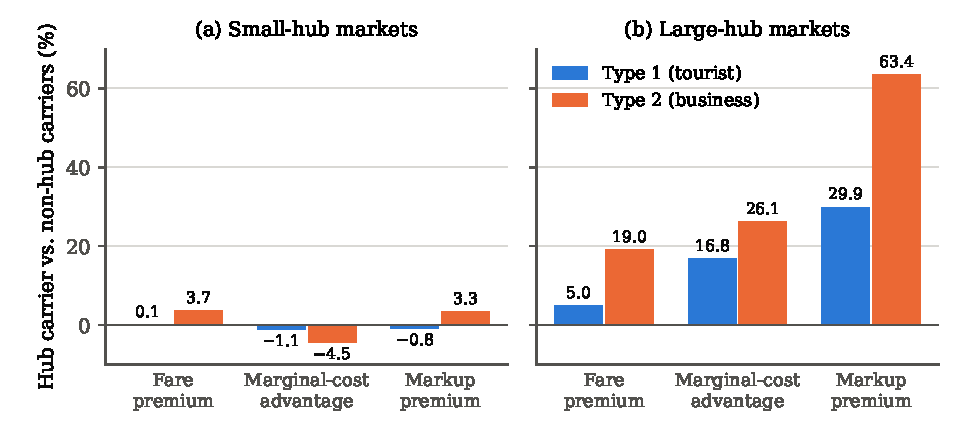
\includegraphics[width=\textwidth]{figures/ch09/bcs_hubpremia.pdf}
\caption{Hub premia by market and traveler type. The fare premium is the percentage by which the hub
carrier's average fare exceeds that of non-hub carriers. The marginal-cost advantage and the markup premium
are defined in \eqref{eq:09-bcs-premia}. Redrawn from the bottom panel of Table~6 of
\citet{BerryCarnallSpiller1996}, based on the column III estimates.}
\label{fig:09-bcs-premia}
\end{figure}

\Cref{fig:09-bcs-premia} plots the premia.\footnote{The text describes a Figure~4 that presents these
results (p.~26, n.~17), but the posted working paper does not contain it. Our figure plots the numbers of
Table~6 and does not reproduce Figure~4.} The pattern supports claims (ii) and (iii). In small hubs the
premia are close to zero for both types. In large hubs the hub carrier earns a substantial premium from
business travelers and a small one from tourists, while enjoying lower marginal cost for both. Business
travelers ``are not just willing to pay the 20\% premia that hub airlines charge,'' they also fly the hub
carrier more often than its rivals (p.~26).

\casehead{No umbrella: the competitive scissor}
The hub carrier's high fares do not protect its rivals. Non-hub carriers in large-hub markets charge less
than non-hub carriers in non-hub markets (\$205 against \$224 for tourists, \$268 against \$296 for business
travelers). They also lose the business travelers, so their passenger mix is more price sensitive (p.~27). Both
blades of the scissor lower their average yield and the profitability of serving the hub airport. This is
claim (iv), and it matches Borenstein's finding of little umbrella effect (\cref{sec:09-borenstein}). The
fare comparison runs across market categories, which the authors warn against elsewhere (p.~25). The
within-market evidence is cleaner: non-hub carriers' business fares are 16\% below the hub carrier's
($\frac{268}{319}=0.84$).

\casehead{A dynamic interpretation}
The authors suggest an explanation, untested in the paper, of two trends after deregulation (p.~27). Once a
carrier builds a major hub at an airport, its rivals see business customers move away and their yields fall.
Marginal carriers then find it profitable to cut service to that city, and airport concentration rises
without any entry barrier. \citet{BruecknerSpiller1994} document this rise. Hubs also give their carriers
price and cost advantages that ease entry out of the hub into new city pairs. That could explain the fall in
concentration at the level of city-pair markets. For empirical models of airline entry they refer to
\citet{ReissSpiller1989} and \citet{Berry1992}.\footnote{The text cites ``Berry (1991)'' here, while the
reference list contains \citet{Berry1992}, the published entry model.}

\subsubsection{Economies of density}

\Cref{tab:09-bcs-dmc} reproduces Table~7, the derivative of leg marginal cost with respect to density
\eqref{eq:09-bcs-dcdq} at column III estimates, for five distances and six densities. With the column III
coefficients the derivative is
\begin{equation}\label{eq:09-bcs-dcdq-III}
\frac{\partial c_\ell}{\partial Q_\ell}=1.584+2(0.164)Q_\ell+3(-0.238)Q_\ell^2-3.891d_\ell+1.270d_\ell^2
+2(0.524)d_\ell Q_\ell .
\end{equation}
Panel B of the table evaluates this formula. It reproduces 29 of the 30 printed cells to within 0.006, which
is rounding. The exception is the cell for 250 miles and density 1.50.\footnote{Table~7 prints $-0.27$ for
250 miles and 150,000 passengers per quarter. Formula \eqref{eq:09-bcs-dcdq-III} gives $-0.031$, which also
fits the neighboring cells (0.568 at density 1.00 and $-0.980$ at 2.00). We treat the printed value as a
typographical error.}

\begin{table}[htbp]
\centering
\begin{threeparttable}
\caption{Derivative of leg marginal cost with respect to density (column III)}
\label{tab:09-bcs-dmc}
\small
\begin{tabular}{@{}lrrrrrr@{}}
\toprule
 & \multicolumn{6}{c}{Leg density (100,000 passengers per quarter)} \\
\cmidrule(l){2-7}
Leg distance & 0.25 & 0.50 & 0.75 & 1.00 & 1.50 & 2.00 \\
\midrule
\multicolumn{7}{@{}l}{\textit{Panel A. As printed in Table 7}}\\
250 miles & 0.794 & 0.808 & 0.733 & 0.568 & $-0.27$ & $-0.980$ \\
500 miles & 0.125 & 0.204 & 0.194 & 0.096 & $-0.369$ & $-1.190$ \\
1,000 miles & $-0.737$ & $-0.527$ & $-0.406$ & $-0.373$ & $-0.576$ & $-1.135$ \\
1,500 miles & $-0.964$ & $-0.623$ & $-0.371$ & $-0.207$ & $-0.148$ & $-0.446$ \\
2,000 miles & $-0.556$ & $-0.084$ & 0.299 & 0.593 & 0.914 & 0.879 \\
\addlinespace
\multicolumn{7}{@{}l}{\textit{Panel B. Computed from the Table 5 column III coefficients}}\\
250 miles & 0.793 & 0.807 & 0.732 & 0.567 & $-0.031$ & $-0.985$ \\
500 miles & 0.124 & 0.203 & 0.193 & 0.094 & $-0.373$ & $-1.196$ \\
1,000 miles & $-0.738$ & $-0.527$ & $-0.407$ & $-0.375$ & $-0.579$ & $-1.141$ \\
1,500 miles & $-0.965$ & $-0.623$ & $-0.372$ & $-0.209$ & $-0.151$ & $-0.451$ \\
2,000 miles & $-0.557$ & $-0.084$ & 0.298 & 0.592 & 0.912 & 0.874 \\
\bottomrule
\end{tabular}
\begin{tablenotes}\footnotesize
\item Notes: \$100 per 100,000 passengers per quarter. A negative entry means economies of density. Panel B
evaluates \eqref{eq:09-bcs-dcdq-III} (our computations). Source:
\citet{BerryCarnallSpiller1996}, Table~7.
\end{tablenotes}
\end{threeparttable}
\end{table}

\begin{figure}[htbp]
\centering
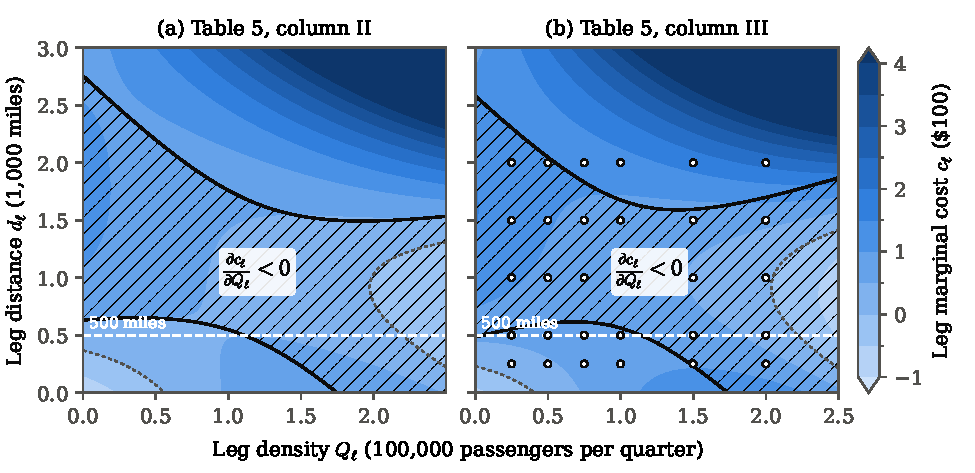
\includegraphics[width=\textwidth]{figures/ch09/bcs_mc_surface.pdf}
\caption{Leg marginal cost over leg density and distance. Shading gives the level of $c_\ell$ in \$100 from
\eqref{eq:09-bcs-mc}, with congestion terms and the product-level constant set to zero. The hatched region,
bounded by the solid curve, has $\frac{\partial c_\ell}{\partial Q_\ell}<0$ (economies of density). Dotted
curves mark $c_\ell=0$, where the polynomial turns negative. The dashed line marks 500 miles, and the dots in
panel (b) are the grid points of \cref{tab:09-bcs-dmc}. Leg densities above 250,000 passengers per
quarter, up to the observed maximum of 455,300, are not shown. Constructed from
\citet{BerryCarnallSpiller1996}, Table~5, columns II and III.}
\label{fig:09-bcs-mc}
\end{figure}

\Cref{fig:09-bcs-mc} redraws the cost surface for columns II and III. The working paper shows the same
surfaces as three-dimensional plots in Figures 1 to 3.\footnote{Figures 1 to 3 are titled ``Col II Table 4''
and ``Col III Table 4,'' while the text says that they correspond to columns II and III. The cost parameters
are in Table~5, so the titles should read Table~5.} The two columns give the same basic shape (p.~27), with
three distance ranges.
\begin{itemize}
  \item Below about 500 miles, marginal cost rises with density up to about 150,000 passengers per quarter
  and then falls (p.~27). In column III the derivative turns negative above a density of 1.48 at 250
  miles and above 1.14 at 500 miles. The introduction's summary of no economies of density below about 500 miles (p.~3)
  therefore holds only up to these densities. The authors explain that over short distances the cruising efficiency of larger aircraft may not make up for
  their higher takeoff and landing costs. Higher density must then be met with more flights.
  \item Between 500 and 1,500 miles there are economies of density at all densities (p.~28). In column III
  the derivative is negative for legs between 617 and 1,589 miles at every observed density, up to
  455,300 passengers per quarter.
  \item Above 1,500 miles, the authors find that marginal cost rises with density except at very low
  densities (p.~28). At 2,000 miles the column III derivative is negative below 55,000 passengers per
  quarter and positive from there to about 284,000. Above that density the negative cubic term in density
  turns it negative again. At 2,000 miles this second sign change lies outside \cref{tab:09-bcs-dmc} and
  \cref{fig:09-bcs-mc}. It lies inside the observed range, whose maximum in \cref{tab:09-bcs-desc} is
  455,300. Such densities are far in the upper tail, since first outbound legs have a mean density of 59,300
  and a standard deviation of 47,500. The derivative also turns negative at high densities inside the
  observed range at every distance from 1,590 miles to the longest observed leg of 2,704 miles. Below
  about 1,870 miles this happens inside the plotted range, where the upper edge of the hatched region in
  panel~(b) of \cref{fig:09-bcs-mc} rises with density. At 1,700 miles, for example, the derivative is
  negative below 95,100 passengers per quarter and again above 200,400. The authors offer two
  explanations for the rising cost (p.~28). Polynomials tend to curl up or down at the corners of the
  data, and the same caution applies to these high-density sign changes. Alternatively, the largest aircraft are
  already in use on long legs, so more density can only be met with more flights.
\end{itemize}
Most leg-carrier combinations in the data lie either under 500 miles or inside the region with economies of
density, as the authors' Figure~3 shows (p.~28). Few legs fall in the long-distance, high-density corner
where marginal cost rises steeply.

The derivatives are large. At 1,000 miles and 100,000 passengers per quarter, the leg's marginal cost
falls at a rate of about \$37 per additional 100,000 passengers, or about \$3.70 per additional 10,000.
Because the derivative steepens with density, doubling density to 200,000 lowers it by about \$64. Average
product marginal costs in Table~6 range from \$91 to
\$133. The authors suspect that the polynomial makes the cost surface ``too curvy,'' so they stop short of
the detailed cost analysis they perform for demand (p.~28). They still read the results as consistent with
economies of density over a wide range. The average market distance in large-hub markets, 842 miles, lies
inside the band where column III implies economies of density at all densities. The cost advantage of large
hub carriers in Table~6 is consistent with this.

The absence of density economies on short legs below about 150,000 passengers per quarter is the
``Southwest effect'' (p.~28). A non-hubbing carrier that offers frequent service on such legs loses little
by not hubbing, because a hub would not lower its costs there. The authors infer that Southwest's success may reflect a cost niche as well as lower
labor costs. They add that Southwest's move toward national service takes it into the distance range where
density economies, and hence hubs, may be more efficient (p.~3, n.~6). In terms of \cref{ex:09-hubcost},
short legs below that density behave like $\gamma\ge1$, where hubbing never saves cost, and legs of 600 to 1,600 miles behave
like $\gamma<1$.

\subsection{Conclusions, limitations, and contribution}\label{sec:09-bcs-conclusions}

\casehead{The authors' conclusions}
The conclusions (pp.~28--29) restate the claims of \cref{sec:09-bcs-question} with their evidence. The data
and model identify two types of travelers with sensible business and tourist tastes (Tables 4 and 5).
Economies of density imply that hubs save costs (Tables 5 and 7). Hubs let carriers charge a premium, but the
ability to raise prices is much greater for business travelers. Out of large hubs these travelers pay about
20\% more, while the premium for tourists is about 5\% or less (Table~6). The authors argue that the welfare
consequences of the premium ``need not be negative'' (p.~29). Business travelers receive a higher-quality product in observed and
unobserved characteristics. They are a larger share of hub carriers' passengers, and their demand is
inelastic. Aside from the issues the model leaves out, ``the negative welfare consequences of hubs appear to
be rather small'' (p.~29).

\casehead{From tables to economic inferences}
The chain of inference has five links. Table~3 shows that reduced-form coefficients mix markups and costs,
which motivates the structural model. Table~5 rejects the logit and finds two price coefficients an order of
magnitude apart. The other type-specific coefficients and the Table~4 composition give the second type
business tastes. The pricing condition converts demand estimates into markups and hence into marginal costs.
Table~6 then compares hub and non-hub carriers within markets, and Table~7 shows where costs fall with
density. Every inference after the first depends on the demand model and on static Nash pricing. No formal
test accompanies the Table~6 premia or the Table~7 derivatives.

\casehead{Alternative interpretations the authors consider}
The authors flag several alternatives themselves. Part of a measured markup may be a shadow price of capacity
(p.~14). Hubs may lower fixed costs, which the model cannot detect (pp.~5 and 14). Pricing may be dynamic,
through yield management, or collusive (pp.~15 and 28). The curvature of the cost surface may be an artifact of the
polynomial (p.~28). Network structure may affect entry and exit, and frequent-flyer programs and travel-agent
commissions may exploit agency problems between the traveler and the payer, which the model does not
represent (p.~28).

\casehead{Limitations}
Several further limitations follow from the design.
\begin{itemize}
  \item The welfare claim is informal. A formal calculation would compute each type's expected surplus from
  the nested logit inclusive value (\cref{ch:logit}). It would then solve for counterfactual prices and
  densities without hubs and compare the two (\cref{ch:newgoods}). Because densities and costs are linked across the
  network, the counterfactual would require re-solving the equilibrium in all markets at once.
  \item The marginal costs are residuals of the pricing condition. If hub carriers do not price as static
  Nash competitors, the conduct error is absorbed into marginal cost. The measured cost advantage of hub
  carriers then mixes cost with conduct, the problem studied in \cref{ch:conduct}.
  \item Ticket restrictions enter only through $\xi$, which is assumed mean independent of the observed
  characteristics and of the network. If hub carriers systematically offer less restricted tickets out of
  their hubs, part of the measured hub taste is a taste for restrictions.
  \item The type distribution has two points and no heterogeneity within a type. The nest groups all flights
  together, so flights of the same carrier or from the same airport are no closer substitutes than others.
  \item Shares are measured with large sampling error, which is not corrected.
  \item Southwest, the carrier behind the ``Southwest effect,'' is absent from the data. The short-haul cost
  estimates come from the other carriers.
  \item The definition of a hub is not documented in the available file beyond a list referred to in the
  Table~6 notes, and HUBSIZE has no natural unit.
  \item The analysis uses one quarter of data, so it cannot study how hubs form, a limitation the authors
  acknowledge when they leave the dynamic interpretation untested.
\end{itemize}

\casehead{Contribution}
The paper is the first to separate the cost advantages of hubs from hub markups within one structural model.
It shows that market-level data can identify discrete consumer types, here with closed-form shares and
without simulation. It also estimates network marginal costs from spoke densities without accounting cost
data, through the pricing condition. Its substantive findings explain why the hub premium falls on business
travelers and why it creates no umbrella for rivals.

\begin{table}[htbp]
\centering
\caption{Identification and counterfactual map of Berry, Carnall and Spiller (2006)}
\label{tab:09-bcs-map}
\footnotesize
\renewcommand{\arraystretch}{1.1}
\begin{tabularx}{\textwidth}{@{}>{\raggedright\arraybackslash}p{2.6cm}>{\raggedright\arraybackslash}X@{}}
\toprule
Observed data & DOT round-trip tickets for the fourth quarter of 1985, with segment traffic from DB27R.
  Fares, shares and characteristics of 122,871 carrier-itinerary-fare products in 14,122 directional
  city-pair markets. \\
\addlinespace
Latent objects & Two traveler types and their population shares, product quality $\xi_{jt}$, cost shocks,
  leg marginal costs and markups. \\
\addlinespace
Estimated parameters & The type-1 probability $\psi$ and type-specific price and taste coefficients,
  including the hub tastes $\beta^h_r$. The nesting parameter $\sigma$, the market-size factor $\kappa$, and
  the coefficients $\chi$ of leg costs in distance and density. \\
\addlinespace
Identifying variation & The moments \eqref{eq:09-bcs-moments}, with own and rival product characteristics
  and endpoint population and network variables as instruments. Within-carrier differences between cheap
  and expensive products at hub and non-hub origins separate the types' hub tastes \eqref{eq:09-bcs-hubid}. \\
\addlinespace
Maintained assumptions & A two-type nested logit, exogenous characteristics and networks, static
  multiproduct Nash pricing, and a polynomial leg cost in distance and density. \\
\addlinespace
Counterfactual and what it holds fixed & No new equilibrium is computed. Markups and marginal costs are
  evaluated at observed fares, and hub premia compare hub and non-hub carriers within markets. \\
\addlinespace
Conclusion & Out of large hubs business travelers pay about 20 percent more and tourists about 5 percent or
  less. Hub carriers also have lower marginal costs, with density economies on longer routes. The
  decomposition rests on static Nash pricing. \\
\addlinespace
One limitation & Marginal costs are residuals of the pricing condition, so any departure from Nash pricing
  is absorbed into measured cost. \\
\addlinespace
Source and our additions & The tables come from the 1996 working paper. \Cref{ex:09-twotypes},
  \cref{prop:09-composition-markup,lem:09-fm-contraction}, the factor structure \eqref{eq:09-bcs-factor}
  and the sampling-error calculation are ours. \\
\addlinespace
Tools in the appendices & \Cref{sec:A-gmm,sec:B-fixedpoint}. \\
\bottomrule
\end{tabularx}
\end{table}

\section{Synthesis: what three methods teach about hub premia}\label{sec:09-synthesis}

The three papers of this chapter study the same industry, use the same public data source and ask related
questions. Their methods differ: pricing regressions, an event study of stock returns, and a structural model
of demand, cost and pricing. This section compares what each method identifies, asks what each paper adds
given the other two, assembles the evidence on the sources of hub premia, and applies it to merger policy.

\subsection{Three designs side by side}\label{sec:09-synthesis-designs}

\Cref{tab:09-compare} summarizes the three designs. For each paper the rows give the observation, the
dependent variable, the key regressors, the source of identification and the headline result.

\begin{table}[htbp]
\centering
\begin{threeparttable}
\caption{Three designs for one question}
\label{tab:09-compare}
\footnotesize
\begin{tabularx}{\textwidth}{@{}>{\raggedright\arraybackslash}p{1.9cm}>{\raggedright\arraybackslash}X
  >{\raggedright\arraybackslash}X>{\raggedright\arraybackslash}X@{}}
\toprule
 & \citet{Borenstein1989} & \citet{WhinstonCollins1992} & \citet{BerryCarnallSpiller2006} \\
\midrule
Method & Reduced-form pricing regressions & Event study of stock returns & Structural demand, cost and
  pricing model \\
\addlinespace
Data and period & DOT ticket sample (DB1A), 1987Q3, with Service Segment and Nonstop Market data & 24 People
  Express entry announcements in 1984--1985, daily returns of 20 carriers, airline schedules, DB1A first
  quarters of 1984--1986 & DB1A round trips, 1985Q4, with segment traffic from DB27R \\
\addlinespace
Observation & One randomly chosen qualifying carrier per airport-pair route (3,591 routes, and 1,508 for the
  relative-price equation) & Carrier and trading day & Carrier-itinerary-fare product in a directional
  city-pair market (122,871 products in 14,122 markets) \\
\addlinespace
Dependent variable & Logs of the 20th, 50th and 80th percentile fares, and log fare ratios of two carriers &
  Daily excess return & Shares and fares, through the inversion ($\xi$) and the pricing condition
  ($\omega$) \\
\addlinespace
Key regressors & Route share, endpoint share, route and endpoint Herfindahls, cost and quality controls,
  airport effects & Annualized seat-miles on the entered pair (SM) and at other airports (OSM), departures
  at the entered airport (EPORT), firm effects & Fare, DIRECT, HUBSIZE, TEMPDIFF, TRIPS-D (type-specific),
  distance, congestion, leg distance-density polynomial \\
\addlinespace
Identification & 2SLS with constructed instruments (GENPSH, IRUTHERF), carrier effects, differencing
  within routes & Timing of announcements and differences in carriers' exposure, estimated by SUR & GMM with
  exogenous characteristics, network and rival-product instruments, and Nash pricing \\
\addlinespace
Headline & A carrier with 70\% of a route charges 2\% to 12\% more than rivals with 10\%. Endpoint dominance
  raises fares, more at the high end. Little umbrella effect & Incumbents lose \$3.7 to \$6.5 million per
  incumbent and event. Incumbent fares fall about 35\% after entry, relative to markets not entered.
  Contestability rejected & Large-hub
  premium of 19\% for business travelers and 5\% for tourists, with lower marginal cost. Density economies
  at medium distances. No umbrella \\
\addlinespace
Main maintained assumptions & Exclusion of the instruments. Shares not proxies for unobserved quality &
  Efficient markets, correct dating, no confounding news, unanticipated events & Two-type nested logit,
  exogenous characteristics and network, static Nash pricing, polynomial costs \\
\bottomrule
\end{tabularx}
\begin{tablenotes}\footnotesize
\item Notes: Sources are \citet[Tables 2--4]{Borenstein1989}, \citet[Tables 1 and 3]{WhinstonCollins1992}
and \citet[Tables 1 and 5--7]{BerryCarnallSpiller1996}. The People Express events and the 20 carriers are
described in \cref{sec:09-wc}.
\end{tablenotes}
\end{threeparttable}
\end{table}

All three papers reject perfect contestability, through different predictions of \cref{sec:09-contest-fail}.
Borenstein finds that fares depend on route and airport dominance holding costs fixed, against prediction
(C1). Whinston and Collins find that entry announcements reduce incumbents' values, against (C2). By
\cref{prop:09-valueloss}, this reveals route-specific profits or sunk costs. Borenstein's route-share and
route-concentration effects survive when POTCOMP controls for potential competitors (Panel B of
\cref{tab:09-bor-main}), against (C3). The small POTCOMP coefficient alone does not test (C3), because under
perfect contestability fares equal average cost whatever the number of potential entrants. Berry, Carnall and Spiller find large markups where the hub carrier
also has lower costs, against (C4), with the caveat of \cref{rem:09-markups-profits} that markups are not
profits. The rejections come from three different kinds of evidence, which makes the verdict robust.

\subsection{What each method identifies}\label{sec:09-synthesis-identify}

Borenstein's regressions identify a conditional correlation between dominance and fares. Under the exclusion
restrictions on his instruments, the route-share coefficient measures how a carrier's fare responds to its
share. By \eqref{eq:09-pricing-approx}, this response is a markup effect only if the share does not proxy for
lower cost or higher quality. The regressions cannot tell a high price that reflects market power from one
that reflects a better product, because they contain no model of either. Their strength is breadth and
transparency: thousands of routes and a specification any reader can check.

Whinston and Collins identify a bound. By \cref{prop:09-valueloss}, the market value an incumbent loses at an
entry announcement is at most the sum of its pre-entry route profits and its sunk costs. A positive loss
proves that one of the two is positive. The design needs no model of demand or costs and no controls for
route characteristics, because the stock market prices the route's prospects. It identifies the existence and
a lower bound of route-specific rents, and how localized they are. It cannot say whether the rents come from
pricing, costs or quality, and it cannot separate profits from sunk costs.

Berry, Carnall and Spiller identify primitives: type-specific demand, product markups and leg marginal costs.
With these they can separate the fare premium into a markup and a cost component, and in principle simulate
counterfactuals. The price is a set of functional forms and behavioral assumptions. The two-type nested logit,
the exogeneity of characteristics and network, static Nash pricing and the cost polynomial all shape the
answer.

\subsection{The contribution of each paper given the other two}\label{sec:09-synthesis-contrib}

Given the other two papers, Whinston and Collins add evidence that does not depend on controls or on an
equilibrium model. Their value losses show that route-level rents exist, which both other papers presume. The
difference between the entered airport pair and other airports in the same city pair shows that airports
within a city are differentiated. Under the assumptions of \eqref{eq:09-wc-did-model}, the 35\% fall in
incumbent fares after entry measures how much of the fare level depends on the absence of a low-fare
competitor.

Given the other two, Berry, Carnall and Spiller add the decomposition and the mechanism. They explain
Borenstein's asymmetry, a dominant carrier with high fares and rivals without, through the sorting of business
travelers. This is the logic of \cref{prop:09-dominance} and \cref{prop:09-composition-markup}. The hub
carrier attracts the inelastic travelers and leaves its rivals with the elastic ones, so rivals cannot raise
their fares. Borenstein's finding that endpoint dominance raises high-end fares about three times as much as
low-end fares anticipates the business travelers' taste for hubs. The density economies show that part of the
hub carrier's markup is financed by lower cost. In large hubs the business fare premium is 19\% of the
non-hub fare, while the markup gain is 32\%.

Given the other two, Borenstein adds the broad pattern. His regressions cover thousands of routes and nine
carriers. They show that carrier-specific dominance of routes and airports predicts fares. Route concentration as
such does not. His airport effects separate scarcity rents, common to all carriers at an airport, from
carrier-specific dominance. His results set the agenda that the other two papers pursue.

Together the papers are more than the sum of their parts, because each covers another's weakness. The
structural model answers the quality confound in Borenstein's regressions. The event study supplies
market-based evidence that does not depend on the structural model's equilibrium assumption. Borenstein's
breadth offsets the narrow sample of 24 events, 22 of them at Newark. The fit is imperfect. The papers use
different periods (1984--1985, 1985Q4, 1987Q3) and different market definitions (airport pairs and city
pairs), and none of them studies the formation of hubs.

\subsection{Sources of hub premia}\label{sec:09-synthesis-sources}

\Cref{tab:09-sources} collects the evidence on five candidate sources of the hub premium. The table shows
which source each method can address. It also shows that no single paper speaks to all five.

\begin{table}[htbp]
\centering
\begin{threeparttable}
\caption{Sources of hub premia: what each paper shows}
\label{tab:09-sources}
\footnotesize
\begin{tabularx}{\textwidth}{@{}>{\raggedright\arraybackslash}p{1.9cm}>{\raggedright\arraybackslash}X
  >{\raggedright\arraybackslash}X>{\raggedright\arraybackslash}X>{\raggedright\arraybackslash}X@{}}
\toprule
Source & \citet{Borenstein1989} & \citet{WhinstonCollins1992} & \citet{BerryCarnallSpiller2006} & Later work \\
\midrule
Lower cost (density economies) & Not identified. Cost controls only & Not measured & Density economies for
  legs of roughly 600 to 1,600 miles, and below about 500 only above about 110,000 to 150,000 passengers. Hub carriers' marginal cost 26\% lower for
  business tickets in large hubs & \citet{BruecknerSpiller1994} on density economies from spoke data \\
\addlinespace
Quality and demand (frequency, nonstop service, network breadth) & Frequency raises fares, more at the high
  end. Cannot be separated from market power & Not separable from rents & Business travelers value
  directness, hub size and frequency far more. Hub carriers' products have higher $\xi$ & \citet{Berry1990}
  on airport presence as differentiation \\
\addlinespace
Market power from dominance & Route and endpoint shares raise own fares. Little umbrella & Route-specific
  rents revealed by value losses & Business markups 63\% higher on hub carriers in large hubs. No umbrella &
  \citet{CilibertoTamer2009}: competitive effects rise with airport presence \\
\addlinespace
Sunk costs, entry barriers and potential competition & Potential competition has a small effect & Losses
  reveal profits or sunk costs. Contestability rejected & Entry and network taken as given &
  \citet{GoolsbeeSyverson2008}: incumbents cut fares when Southwest threatens entry \\
\addlinespace
Scarcity rents (slots, gates) & Airport effects: O'Hare $+3\%$ to $5\%$, Atlanta $+1\%$ to $3\%$, Denver $+2\%$
  to $4\%$. Common to all carriers & Firm effects may include slot values & Congestion raises cost and lowers
  demand. Rents not separated & \citet{CilibertoWilliams2010}: gate control raises fares where gates are
  scarce \\
\bottomrule
\end{tabularx}
\begin{tablenotes}\footnotesize
\item Notes: Borenstein's airport effects are from p.~359 of his article. Details of each paper are in
\cref{sec:09-borenstein}, \cref{sec:09-wc} and \cref{sec:09-bcs}, and of the later work in
\cref{sec:09-synthesis-later}.
\end{tablenotes}
\end{threeparttable}
\end{table}

The table suggests a division of the hub premium. A substantial part of the fare gap between hub and non-hub
carriers reflects quality that business travelers value and lower costs on medium-haul legs. Market power
from dominance is real, but it is concentrated on business travelers and does not spill over to rivals.
Route-specific rents and sunk costs keep potential entry from eliminating it. Scarcity of airport facilities
adds a premium that is common to all carriers at an airport, and control of gates turns it into a source of
carrier-specific advantage.

\subsection{Merger policy: two hypothetical mergers}\label{sec:09-synthesis-mergers}

Consider an antitrust agency reviewing two hypothetical mergers. Merger A combines two network carriers with
large hubs, of the kind represented by Delta and United. Merger B combines two low-cost carriers that fly
mostly point to point, of the kind represented by JetBlue and Southwest. The three papers leave both cases
open. They tell the agency where to look. The formal tools, upward pricing pressure, merger simulation and
retrospective studies, are developed in \cref{ch:mergers}.

\casehead{Merger A: two hub carriers}
Borenstein's results predict higher fares on routes where the merging carriers' combined route share rises,
and at airports where their combined endpoint share rises. The largest effects arise on hub-to-hub routes,
where each carrier competes from its own stronghold. The absence of an umbrella shows that a carrier's dominance
does little to raise its rivals' fares. It does not predict how rivals would respond to a change in ownership. Both that
response and the discipline that rivals impose on the merging carriers depend on diversion and on equilibrium pricing.
Berry, Carnall and Spiller predict that the price effect falls mainly on business travelers. A merger enlarges
the network connected through each hub and so raises each hub's HUBSIZE. By
\cref{prop:09-composition-markup}, that tilts the buyers of the merged carrier's hub products further toward
business travelers and raises markups on the tickets they buy. Tourists would see smaller changes. The same
paper also points to efficiencies. Combining traffic on overlapping spokes raises density, and on legs of
roughly 600 to 1,600 miles that lowers marginal cost. An efficiency defense is therefore plausible for
overlapping medium-haul spokes and weak for short ones. Whinston and Collins show that route-level rents
survive potential competition, so the loss of an actual competitor on overlap routes matters. They also show
how much entry by a low-fare carrier can cut fares. The incumbents' aggressive responses that they document,
however, suggest that such entry is costly and uncertain.

The agency would want the overlapping routes and the airports where both carriers have large shares. It
would want diversion ratios by fare class and the density and distance of the spokes that would be combined.
It would also want a merger simulation with heterogeneous travelers. Remedies that open gates and slots at the hubs speak to the
facility-based advantages that \citet{CilibertoWilliams2010} measure. The papers that matter most for merger A
are Berry, Carnall and Spiller, for the decomposition of the premium into markups and costs, and Borenstein,
for the link between dominance and fares.

\casehead{Merger B: two low-cost carriers}
For merger B the most relevant evidence concerns entry. Under the assumptions of \eqref{eq:09-wc-did-model},
Whinston and Collins find that entry by a low-fare carrier cut incumbents' mean fares by about 35\%. Their
event study finds that it cost each incumbent \$3.7 to \$6.5 million in value per event. A low-cost carrier is a source of discipline, so merging two of them removes an independent low-fare
competitor on overlap routes. \citet{GoolsbeeSyverson2008} show that incumbents cut fares when Southwest
becomes a likely entrant, before it starts flying. The merger would also remove each carrier as a potential
entrant on the other's routes. On the cost side, Berry, Carnall and Spiller find economies of density below
about 500 miles only on dense legs, above about 110,000 to 150,000 passengers per quarter. Combining
short-haul point-to-point networks therefore saves cost through density only where the combined legs are that
dense.
Their cost estimates exclude Southwest, so this inference rests on other carriers' short legs. Borenstein's
dominance results matter less here, unless the merger creates a dominant position at airports where both
carriers concentrate. The agency would want the overlapping routes and the routes where each carrier is a
likely entrant. It would also want estimated entry probabilities and the fare changes on routes where one
carrier entered against the other. The papers that matter most for merger B are Whinston and Collins and, among later work, Goolsbee and
Syverson.

\subsection{Later evidence*}\label{sec:09-synthesis-later}

\casehead{Price dispersion}
\citet{BorensteinRose1994} study the dispersion of fares that one carrier charges different passengers on the
same route. In the working-paper version, the expected absolute difference between the fares of two of a
carrier's passengers on a route averages 36\% of the carrier's mean fare. Dispersion is higher on more
competitive routes, which they interpret as price discrimination in monopolistically competitive markets,
against travelers who are less willing to switch flights or carriers. \citet{GerardiShapiro2009} revisit
the question with a panel from the first quarter of 1993 to the third quarter of 2006. Competition reduces
dispersion, as the textbook theory of price discrimination predicts. The effect is pronounced on routes with a
heterogeneous mix of business and leisure travelers. They attribute the contrast with Borenstein and Rose to
omitted-variable bias in cross-sectional estimates. Both papers rest on the heterogeneity of travelers that
Berry, Carnall and Spiller model as two types.

\casehead{The threat of entry}
\citet{GoolsbeeSyverson2008} use the expansion of Southwest's network to identify routes where the probability
of entry rises abruptly. We cite their NBER Working Paper 11072 (January 2005, revised August 2008), whose
table numbers may differ from those of the published article. A route is threatened when Southwest begins to
serve its second endpoint without yet flying the route. A descriptive probit of Southwest's entry into a route
in a given quarter shows the size of the jump (Table~I). Presence at one endpoint raises the entry probability
only slightly above a baseline near zero. Presence at both raises it by a further factor of about 70, to
18.5\% per quarter (p.~5).

Let $\tau_0$ be the quarter in which Southwest first serves both endpoints of route $t$, and let $\tau_e$ be
the quarter in which it starts flying the route. In this discussion $\tau$ indexes quarters. For incumbent
carrier $f$, the authors estimate the event-study regression
\begin{equation}\label{eq:09-gs}
  y_{ft\tau} = \gamma_{ft} + \gamma_{f\tau} + \sum_{k} \beta_k\,D^{0}_{t\tau k}
  + \sum_{k} \lambda_k\,D^{e}_{t\tau k} + e_{ft\tau}
\end{equation}
(pp.~6--7). The outcome $y_{ft\tau}$ is the passenger-weighted mean log fare, and $\gamma_{ft}$ and
$\gamma_{f\tau}$ are carrier-route and carrier-quarter fixed effects. The threat dummy $D^{0}_{t\tau k}$
equals one when $\tau = \tau_0 + k$ and Southwest does not yet fly the route. It runs from $k = -8$ to
$k = 2$, and one more dummy pools the quarters from $\tau_0 + 3$ on. The entry dummies $D^{e}_{t\tau k}$
mark the quarter $\tau_e$, the two quarters after it, and the quarters from $\tau_e + 3$ on. The omitted
period is the 9th through 12th quarters before $\tau_0$, so each coefficient measures log fares relative to
that baseline. Observations are weighted by passengers, and standard errors are clustered by route-carrier
pair (p.~7).

Column~(1) of their Table~II gives $\hat\beta_0 = -0.186$ (0.073). Since $e^{-0.186} = 0.830$, fares are
about 17\% lower by the quarter $\tau_0$ (p.~8). They begin to fall about three quarters before $\tau_0$.
Southwest announces its arrival at an airport months in advance, and insiders may learn of it earlier
(p.~9). Once Southwest flies the route, fares are 21\% below the baseline, since $e^{-0.237} = 0.789$. By
the end of the window they are over 29\% lower, since $e^{-0.344} = 0.709$ (p.~9). Over half of Southwest's
total effect on incumbents' fares thus occurs before entry. The cuts occur only on threatened routes and not
on routes from nearby airports. This answers the question that Borenstein's potential
competition variable and Whinston and Collins's announcements could only approach. Potential competition does
discipline incumbents when the entrant is credible and the threat is specific to a route.

\casehead{Gates and the hub premium}
\citet{CilibertoWilliams2010} measure the role of airport facilities directly, with data from the competition
plans that major airports must file with the DOT. Our numbers come from the February 2009 author manuscript
(MPRA Paper 38636), then forthcoming in the \emph{Journal of Law and Economics}. The hub premium rises with
the fare. It is below 10\% at the 10th percentile of the fare distribution and almost 25\% at the 90th
(p.~3). Their Table~7 adds the measures of barriers to entry to the fare regression. The premium on tickets
out of a hub then falls from about 12\% to about 6\%, and the premium on tickets into a hub from 12.7\% to
9.3\% (pp.~21--22). In the authors' summary, the premium falls by almost half (p.~22). Control of gates leased on an exclusive basis is
a key determinant. The coefficient on the carrier's share of gates at the origin airport, OwnGatesOrigin, is
0.163. A rise in that share from 10\% to 30\% therefore raises fares by about $0.20 \times 0.163 \approx 3\%$.
Gate control explains high fares only where gates are scarce relative to departures (pp.~23--24). These
results support Borenstein's facility mechanism and fit the
finding of Berry, Carnall and Spiller that the premium falls on high-fare, business tickets.

\casehead{Entry games}
\citet{CilibertoTamer2009} estimate entry games in airline markets without assuming a unique equilibrium,
in the tradition of \citet{Berry1992}. They find heterogeneous competitive effects. The effects of large
carriers differ from those of low-cost carriers and Southwest, and a carrier's competitive effect increases
with its airport presence. Airport presence thus shapes market structure as well as fares, as Berry, Carnall
and Spiller conjecture in their dynamic interpretation.

\casehead{Merger retrospectives}
The airline mergers of the mid-1980s, which motivated much of this literature, have been studied after the
fact, and \cref{sec:11-retro} places these retrospectives among the general methods of merger evaluation.


\section{Bibliographic notes}\label{sec:09-bibnotes}

\citet{Borenstein1989} built on earlier studies of airline pricing. They regressed route fares on route
concentration and cost controls \citep{GrahamKaplanSibley1983,BaileyGrahamKaplan1985,CallKeeler1985,MorrisonWinston1987}. These studies established that fares rise with concentration, against the
contestability benchmark of \citet{BaumolPanzarWillig1982} and \citet{Baumol1982}. \Cref{sec:09-contest}
follows the textbook account of \citet[sec.~8.1]{Tirole1988}. Tirole also presents the critique that prices
adjust faster than entry. He treats the war of attrition as an alternative model of natural monopoly
(sec.~8.1.3). \citet{Levine1987}, who
had regulated, managed and studied airlines, summarizes the view that airport dominance insulates a carrier
from competition \citep[p.~345, n.~3]{Borenstein1989}. \citet{Borenstein1991}
followed his 1989 study with directional city-pair comparisons, which show higher fares on flights out of a
hub than into it. Price dispersion within routes became a separate topic. \citet{BorensteinRose1994} found
more dispersion on more competitive routes in a cross-section, and \citet{GerardiShapiro2009} found the
opposite in a panel.

The cost side of hubbing has its own lineage. \citet{CavesChristensenTretheway1984} estimated economies of
density from an aggregate airline cost function. \citet{BruecknerDyerSpiller1992} and
\citet{BruecknerSpiller1994} moved to marginal costs at the level of flight legs, the approach that
\citet{BerryCarnallSpiller2006} adopt. \citet{BruecknerSpiller1991} study competition and mergers in
hub-and-spoke networks. There, economies of density on a shared spoke link costs across markets
\citep[p.~2, n.~5]{BerryCarnallSpiller1996}. On the demand side,
\citet{MorrisonWinston1986} estimated an early logit model of air travel choices, and \citet{Berry1990}
treated airport presence as a source of product differentiation. The structural approach of
\citet{BerryCarnallSpiller2006} builds on the inversion of \citet{Berry1994} and the estimator of
\citet{BerryLevinsohnPakes1995} (\cref{ch:logit,ch:blp}).

Entry into airline markets is a large literature of its own. \citet{ReissSpiller1989} and \citet{Berry1992}
directly investigate the determinants of entry into city-pair markets \citep[p.~446, n.~1]{WhinstonCollins1992}.
Berry's model treats the number of carriers on a route as an equilibrium outcome.
\citet{CilibertoTamer2009} estimated airline entry games that allow multiple equilibria and heterogeneous
competitive effects. \citet{CilibertoMurryTamer2021} estimate a game in which carriers choose entry and prices
simultaneously, with correlated shocks to demand and cost. Ignoring endogenous entry biases their estimates of
demand elasticities. In a simulated merger of American and US Airways, the outcomes after the merger depend on
how the merged firm's characteristics are modeled. Their framework addresses a limitation of all three papers
of this chapter, none of which models how carriers choose the routes they serve (\cref{sec:09-synthesis}). \citet{GoolsbeeSyverson2008} studied how incumbents respond to the threat of entry by
Southwest, and \citet{CilibertoWilliams2010} measured how control of gates sustains the hub premium. The
event-study method that \citet{WhinstonCollins1992} adapt goes back to \citet{FamaEtAl1969}. Early uses in
regulation include \citet{Schwert1981} and \citet{Rose1985}, and \citet{MacKinlay1997} gives a survey. Event
studies of mergers are treated in \cref{sec:11-retro-event}.

The airline mergers of the mid-1980s were studied after the fact by \citet{Borenstein1990},
\citet{KimSingal1993} and \citet{Peters2006}. \Cref{ch:mergers} places these retrospectives among the
general methods of merger evaluation. On the collusion side, \citet{Miller2010} asks whether the settlement
of the airline tariff publishing case reduced coordination among carriers (\cref{sec:13-atpco}). Dynamic
models of entry, network formation and competition among airlines go beyond the scope of this edition.

\section{Exercises}\label{sec:09-exercises}

\begin{enumerate}[label=\arabic*., leftmargin=*, itemsep=6pt]

\item \emph{A contestable natural monopoly.} Let $C(q)=F+cq$ for $q>0$ and $C(0)=0$, and let market demand
be $Q(p)=A-p$, with $A>c$ and $(A-c)^2>4F$.
\begin{enumerate}[label=(\alph*)]
\item Derive the sustainable price $p^c$ of \cref{prop:09-contest-monopoly} as a function of $(A,c,F)$.
Verify that it equals average cost at the quantity demanded and that it gives $7-\sqrt{17}$ when $A=12$,
$c=2$ and $F=8$.
\item Show that $p^c$ falls toward $c$ as $F\to0$. Compute the deadweight loss at $p^c$ and at the monopoly
price, and explain why the first is the smallest loss compatible with zero profit.
\item Now set $F=0$ and let entry require a sunk investment $K$. The incumbent charges the monopoly price,
and demand and profits are monthly flows. An entrant that slightly undercuts the incumbent earns the monopoly
profit per month until the incumbent responds, and nothing afterward. With $A=12$, $c=2$, $K=100$ and a
monthly discount factor of $0.99$, find the shortest response lag $T$, in months, at which entry pays.
Relate your answer to \cref{prop:09-fragility}.
\item Let instead $C(q)=1+q^2$ for $q>0$, with $C(0)=0$, and $Q(p)=A-p$. Find the efficient scale and the
minimum average cost. For which values of $A$ does \cref{prop:09-nonexist} imply that no configuration is
sustainable? At $A=3.8$, find the single firm's break-even price at the right crossing and the profit of
the entry plan used in the proof of the proposition.
\end{enumerate}

\item \emph{Dominance without an umbrella.} Consider the logit route market of \cref{ass:09-logit} with two
carriers and an outside good, $\alpha=1$ (prices in \$100), $c_1=c_2=1$ and $\delta_2=1$.
\begin{enumerate}[label=(\alph*)]
\item Using the single-equation reduction in the proof of \cref{prop:09-dominance}, compute the Bertrand
equilibrium for $\delta_1\in\{1,2,3\}$. Check your answers against $p_1=p_2=2.227$ at $\delta_1=1$ and
$p_1=2.867$, $p_2=2.148$ at $\delta_1=3$.
\item Verify each claim of \cref{prop:09-dominance} at these points, and compute the route Herfindahl index of
inside shares at each.
\item Regress $\ln p_1-\ln p_2$ on $s_1-s_2$ across the three points. Compare the slope with the
approximation of \cref{cor:09-relprice}, and explain what it implies for the sign of the route-share
coefficient in Borenstein's relative-price equation \eqref{eq:09-bor-rel}.
\end{enumerate}

\item \emph{Reading Borenstein's estimates.}
\begin{enumerate}[label=(\alph*)]
\item Use the 2SLS estimates with POTCOMP in Panel B of \cref{tab:09-bor-main}. For each fare percentile,
compute the fare gap between a carrier with 70\% of a route and rivals with 10\% each. Compare your numbers
with those of the main specification.
\item On a route, carrier 1 has 40\% of the passengers and three rivals have 30\%, 20\% and 10\%. The two
smallest rivals merge. Compute the change in the route Herfindahl index and the implied changes in carrier
1's three fares, holding its share fixed. Explain why the calculation holds the share fixed and why this
matters for reading $\phi_4$ as an umbrella effect.
\item Derive \eqref{eq:09-irutherf} and show that the rescaled rival shares leave the Herfindahl index of
the traffic not carried by $f$ unchanged.
\item Following \cref{rem:09-share-coef}, compute the value of $\bar\eta=\eta_0+\eta_1\bar H$ implied by
each 2SLS route-share coefficient if the route elasticity is $\varepsilon=2$. What outside information would discriminate between
this reading and a Cournot reading?
\end{enumerate}

\item \emph{Event-study algebra.}
\begin{enumerate}[label=(\alph*)]
\item Two carriers have equity values of \$250 million and \$2.5 billion. Compute the dollar loss each would
suffer under a common abnormal return of $-1\%$. Explain why Whinston and Collins prefer the dollar
formulation \eqref{eq:09-wc-dollar}.
\item Using $\lambda_{SM}=-0.0109$, the average incumbent's 7,100 weekly seats and the average distance of
892 miles, compute the implied loss per incumbent. Compare it with the \$3.7 million reported in the paper.
Show that the gap can arise because the mean of a product differs from the product of the means, and state
the sign of the covariance it requires.
\item Three incumbents are hit by the same announcement, and their abnormal returns have pairwise
correlation $0.5$. By what factor does the variance of their average abnormal return exceed the variance
computed under independence?
\item If investors had assigned probability $0.4$ to entry before the announcement, what true loss per
incumbent corresponds to a measured loss of \$3.7 million (\cref{rem:09-anticipation})?
\end{enumerate}

\item \emph{People Express as a difference in differences.} Use Panel A of \cref{tab:09-wc-t34}.
\begin{enumerate}[label=(\alph*)]
\item Compute the two difference-in-differences estimates of the effect of entry on the mean incumbent price
and their average.
\item Compute the pooled two-sample $t$ statistic for the 1984--85 contrast, reading the reported standard
deviations first with divisor $n-1$ and then with divisor $n$. Compare both with the printed value of 2.5.
\item State the identifying assumptions of \eqref{eq:09-wc-did-model}. Use the 1985 cohort's change in
1984--85 and the 1984 cohort's change in 1985--86 to assess them.
\item Explain why the quantity and capacity columns are hard to reconcile with Cournot competition, using
\eqref{eq:09-br-slope}.
\end{enumerate}

\item \emph{Who pays the hub premium?} Use the column III estimates of \cref{tab:09-bcs-demand}.
\begin{enumerate}[label=(\alph*)]
\item Compute an approximate standard error for type 2's willingness to pay for HUBSIZE by the delta method,
ignoring the covariance between the two estimates. Is the ranking of the two types' willingness to pay
robust to this imprecision?
\item By \cref{rem:09-fm-extensions}, a single-product markup is close to $\frac{1-\sigma}{\bar\alpha_j}$
when within-nest shares are small. Compute this approximation for a product whose buyers have the
composition of hub carriers' passengers in large-hub markets (33.0\% type 2) and of non-hub carriers'
passengers there (23.2\% type 2).
\item Compare your answers with the average markups $F-M$ implied by \cref{tab:09-bcs-hub}. Explain why
the approximation at the average buyer composition understates the average markup. (Note that $\frac{1}{\bar\alpha}$
is convex in $\Pr(2\mid j)$.)
\end{enumerate}

\item \emph{Economies of density.} Use the column III cost estimates of \cref{tab:09-bcs-cost}.
\begin{enumerate}[label=(\alph*)]
\item Write the leg marginal cost polynomial and derive $\frac{\partial c_\ell}{\partial Q_\ell}$.
\item Reproduce three cells of \cref{tab:09-bcs-dmc} and identify the printed cell that the formula does not
reproduce.
\item At 250 miles, find the density at which the derivative changes sign. At 2,000 miles, find the density
above which marginal cost rises with density.
\item Discuss what the sign pattern implies for hubbing on short and on medium-haul routes, and connect it to
the cost ratio $\frac{2n^\gamma}{n+1}$ of \cref{ex:09-hubcost}.
\end{enumerate}

\item \emph{An acquisition at a hub.} A network carrier that dominates a hub airport proposes to acquire a
low-cost carrier. The low-cost carrier flies point to point, and a third of its departures use the
acquirer's hub. Drawing on the three papers of this chapter and on \cref{sec:09-synthesis}, write a short
memo to an antitrust agency. Identify the travelers and routes most likely to face higher fares. State the
efficiencies the merging parties could claim and how credible they are. Explain what the agency should
infer from the absence of an umbrella effect. Name the additional evidence you would request, and say which
paper's method would best analyze it.

\end{enumerate}
